\documentclass[TS]{sesamanuel}

% modifications dans la classe (fichier sesamanuel.cls) :
% 	1) ligne 2873, la ligne de remise à zéro du compteur de chapitre a été commentée pour "themaG"
% 	2) création d'une boîte à connaître à la ligne 3471
%	3) ligne 2141 : définition de trois couleurs utilisé par les anciennes figures libreoffice
%	4) ligne 179 et 180 ajout de 2 lignes pour utiliser la police pazocal qui modifie les caractères calligraphiés en mode math
%		du coup : \mathcal{C} donne un C fortement calligraphié et \pazocal{C} donne l'habituel C calligraphié de mathcal
%	5) suppression du texte et du logo dans le titre des QCM d'autoévaluation "Ressources dispo sur sesamaths..." :
%		lignes 3117 et 4396 : commande \StringManuel est commentée
%		lignes 3122 et 4401 : je n'ai pas supprimé le \LogoManuel (une @) mais j'ai changé sa couleur de U4 à Blanc (à la ligne 2702)

% modifications dans le fichier commandesTikZ :
% lignes 31 et 32 pour ajouter la commande \circled qui entoure un caractère


% a priori, après l'impression du livre, tout ce fichier devrait être
% fusionné avec la classe principale, dernière version

\AtBeginDocument{\color{Noir}}

\renewcommand*\StringPrerequis{Connaissances
  n\'ecessaires \`a ce chapitre}

\usepackage{textcomp,pgfplots}
% standalone ne gère pas graphicspath... hum...
\newcommand{\standalonepath}[1]{#1}
% Au début de chaque chapitre on redéfinira cette commande en
% indiquant le chemin

\frenchbsetup{og=«,fg=»,}

\renewcommand\PrefixeCorrection{Corrections/}
\DeclareRemLike{intuition}{Idée intuitive}
\DeclareRemLike{exemples}{Exemples}


\newcommand*\StringExemples{Exemples}
\makeatletter
\newcommand*\smc@cartoucheexemples{% au pluriel
  \begin{pspicture}(-\ExempleVRuleWidthFrame,0)
                 (\ExempleWidthFrame,\ExempleHeightFrame)
    \psframe*[linewidth=0pt,linecolor=ExempleEdgeFrameColor]
             (-\ExempleVRuleWidthFrame,-\ExempleHRuleWidthFrame)
             (\ExempleWidthFrame,\ExempleHeightFrame)
    \psframe*[linewidth=0pt,linecolor=ExempleBkgFrameColor]
             (0mm,-0mm)(\ExempleWidthFrame,\ExempleHeightFrame)
    \rput[B](\dimexpr\ExempleWidthFrame/2,0){%
      \ExempleTitleFont
      \textcolor{ExempleTitleColor}{\StringExemples}%
    }
  \end{pspicture}%
}

\newenvironment{exemples*1}[1][]{%
  \par\addvspace{\BeforeExempleVSpace}
  \let\correction\smc@one@exemplecorrection
  \let\itemize\smc@exempleitemize
  \let\enditemize\endsmc@exempleitemize
  \let\colitemize\smc@exemplecolitemize
  \let\endcolitemize\endsmc@exemplecolitemize
  \let\enumerate\smc@exempleenumerate
  \let\endenumerate\endsmc@exempleenumerate
  \let\colenumerate\smc@exemplecolenumerate
  \let\endcolenumerate\endsmc@exemplecolenumerate
  \let\partie\smc@nopartie
  \let\exercice\smc@noexercice
  \let\endexercice\endsmc@noexercice
  \let\corrige\smc@nocorrige
  \let\endcorrige\endsmc@nocorrige
  \def\smc@currpart{Exemple}%
  \hspace*{\dimexpr \SquareWidth*3}%
  \color{ExempleRuleColor}%
  \vrule width \RuleWidth
  \hspace*{\dimexpr \SquareWidth-\RuleWidth}%
  \minipage[t]{\dimexpr\linewidth-\SquareWidth*4-\ExtraMarginRight}
    \smc@cartoucheexemples
    \space
    \color{Noir}%
    \ignorespaces
}
{%
  \endminipage
  \par
}

\DeclareRemLike{consequence}{Conséquence}
\DeclareRemLike{rappel}{Rappel}
\DeclareRemLike{valeurspart}{Valeurs particulières}
%\DeclareRemLike{theoreme}{Théorème}
% \NewThema{SP}
%          {sp}
%          {stat. et probabilités}
%          {Stat. et probabilités}
%          {STATISTIQUES\\ PROBABILITÉS}
%          {PartieStatistique}
%          {PartieStatistique}

\NewThema{A}
         {a}
         {analyse}
         {Analyse}
         {ANALYSE}
         {PartieFonction}
         {A3}


% Attention, il faudra ajouter un renewcommand \ListeMethodesThemes
% pour afficher la liste des méthodes à la fin du livre

% Si ils veulent changer la couleur du numéro des exos des
% auto-évaluations il faudra aller voir
% \colorlet{CorrigeNumExerciceFrameBkg}{J1}
 
\newcommand{\N}{\mathbb{N}} 
\newcommand{\R}{\mathbb{R}}
\newcommand{\Z}{\mathbb{Z}}
\renewcommand{\cfrac}[2]{{\displaystyle\frac{%
  \vrule height10pt depth0pt width0pt #1}{#2}}%
  \kern-\nulldelimiterspace}
%\usepackage{casio-fx,ti83symbols}

\newcommand\renvoimethode[1]{%
  Méthode \ref{#1}, p.~\pageref{#1}%
}

\newcommand*\calculatrice{%
  \psframebox[framesep=1pt,linewidth=\LogoLineWidth,
              linecolor=TiceLineColor, fillstyle=solid,
              fillcolor=TiceBkgColor, framearc=0.6]{%
    \TiceFont
    \textcolor{TiceTextColor}{CALC}%
  }
}
\newcommand\calc{\calculatrice}

% Chapitre G1 et G3
\newcommand{\covec}[2]{\left(\begin{array}{c} #1\\#2\end{array}\right)}

% Chapitre G2
\usepackage{tipa}
\newcommand{\arc}[1]{%
  \setbox9=\hbox{#1}%
  \ooalign{\resizebox{\wd9}{\height}{\texttoptiebar{\phantom{A}}}\cr#1}}

% Chapitre A4


\DeclareMathOperator{\e}{e}
\renewcommand{\cosh}{\operatorname{ch}}
\renewcommand{\sinh}{\operatorname{sh}}
\renewcommand{\tanh}{\operatorname{th}}

\newcommand*{\StringLEMM}{LEMME\footnote{Un \MotDefinition{lemme}{} est un résultat préliminaire ou  intermédiaire qui intervient parfois dans la preuve d'un théorème lorsqu'elle est un peu longue.}}
\newcommand*{\StringLEMME}{LEMME}
\DeclareDefLike{lemme}{\StringLEMME}
\DeclareDefLike{lemm}{\StringLEMM}

\newcommand*{\StringPROPRIETA}{PROPRIÉTÉ (admise)}
\DeclareDefLike{proprieta}{\StringPROPRIETA}

\usepackage{wrapfig}

% Environnement général pour toutes les fiches
\newcommand\AnnexeTICE{%
  \ChangeAnnexe{C2}{A1}{G1}{Blanc}%
  \annexe{}%
}
% Déclaration de l'environnement pour une fiche
\DeclareTPLike{ficheTICE}{Fiche}
              {TPTopColor}
              {TPBottomColor}
              {TPTitleColor} 
% Définition d'une commande \souspartie pour les besoins de la fiche
% TICE. C'est la commande \partie un peu revue. Je crée les mêmes
% paramètres de contrôle que pour TPPartie en mettant TPSousPartie à
% la place.

\colorlet{TPSousPartieColor}{J1}
\colorlet{TPSousPartieBkgColor}{C2}
\colorlet{TPSousPartieNumColor}{Blanc}
\newcommand*\TPSousPartieFont{\fontsize{10}{12}\sffamily\bfseries}
\def\BeforeTPSousPartieVSpace{3mm plus1mm minus1mm}
\def\AfterTPSousPartieVSpace{0mm plus1mm}
\edef\TPSousPartieHSep{\the\dimexpr\ItemRuleWidth+1.5mm}

\newcommand*\souspartie[1]{%
  \colorlet{smc@curr@partiecolor}{TPSousPartieNumColor}%
  \colorlet{smc@curr@partiebkgcolor}{TPSousPartieBkgColor}%
  \let\smc@curr@partiefont\TPSousPartieFont
  \par\addvspace{\BeforeTPSousPartieVSpace}
  \leavevmode
  \psframe*[linecolor=smc@curr@partiebkgcolor]
           (0,\ItemRuleDepth)(\ItemRuleWidth,\ItemRuleHeight)
  \hspace*{\TPSousPartieHSep}%
  \textcolor{TPSousPartieColor}{\TPSousPartieFont #1}
  \par\nobreak\addvspace{\AfterTPSousPartieVSpace}
}%

\newcommand\RoseItalTice[1]{\emph{\textcolor{C2}{#1}}}

%%% La présentation d'un texte en vis à vis d'une image n'est pas tout
%%% à fait un habillage et la répétition de tels éléments risque de
%%% poser des problèmes. Il vaut mieux se faire son propre « habillage
%%% »
\newcommand\ImageDroite[2]{%
  % #1 = texte
  % #2 = image (ou autre)
  \setbox4=\hbox{#2}%
  \dimen4=\dimexpr\ht4+\dp4-0.7\baselineskip
  \par
  \begin{tabularx}{\linewidth}{@{}Xc@{}}
    #1 & \raisebox{-\dimen4}{#2} %\box4
  \end{tabularx}
  \par
}
\newcommand{\commandetice}[1]{%
  \bgroup
  \shorthandoff{;:!?}%
  \texttt{#1}%
  \egroup
}

\newcommand\touchecalc[1]{%
  \tikz[baseline=-0.5ex]{\node at (0,0) [rounded corners = 2pt, draw, line width=.25pt]
    {\footnotesize\textsf{#1}}}%
}

\DeclareFontFamily{U}{tipa}{}
\DeclareFontShape{U}{tipa}{m}{n}{<->tipa10}{}
\newcommand{\arc@char}{{\usefont{U}{tipa}{m}{n}\symbol{62}}}%

\newcommand{\overarc}[1]{\mathpalette\arc@arc{#1}}

\newcommand{\arc@arc}[2]{%
  \sbox0{$\m@th#1#2$}%
  \vbox{
    \hbox{\resizebox{\wd0}{\height}{\arc@char}}
    \nointerlineskip
    \box0
  }%
}

% Pour A2

\def\psThomae{\pst@object{psThomae}}
\def\psThomae@i(#1,#2){%
   \begin@ClosedObj
   \addto@pscode{
     \psk@dotsize
     1 1 500 {
       dup
       /ipSave ED
       /ip ED
       1 1 500 {
         dup
         /iqSave ED
         /iq ED
         {
           iq 0 le { exit } if
           ip iq mod
           /ip iq def
           /iq ED
         } loop
         ip 1 eq {
           \psk@dotsize
           \@nameuse{psds@\psk@dotstyle}
           \pst@usecolor\pslinecolor ipSave iqSave div 1 iqSave div 
\tx@ScreenCoor
           2 copy moveto Dot
         } if
       } for
     } for
   }%
   \end@ClosedObj%
}

\renewcommand\smc@AfficheListeMethodesTheme[2]{%
  \expandafter\ifx\csname ifsmc@lom#1\endcsname\iftrue
    \csname smc@thema#2Color\endcsname
    \expandafter\smc@bandeaulistemethodes
      \expandafter{\csname StringListeMethode#2\endcsname}
    \ifnum \smc@NombreColonnesListeMethodes=\@ne
      \@starttoc{lom#1}
    \else
      \begin{multicols}{\smc@NombreColonnesListeMethodes}
        \@starttoc{lom#1}
      \end{multicols}
    \fi
  \fi
  \newpage
}
\fancypagestyle{empty}{%
  \fancyhead{}
  \fancyfoot{}
} 

\renewcommand*\AfficheCorriges[1][\NombreColonnesCorriges]{%
  \clearpage
  \label{toutes-solutions}
  \pagestyle{corrige}
  \thispagestyle{firstcorrige}
  \rput[Bl](0,9mm){\CorrigeTitleFont \MakeUppercase{\StringCorriges}}
  \vspace*{-5mm}
  \begingroup
  \columnsep \dimexpr \SquareWidth*2
  \columnseprule \CorrigeRuleWidth
  \def\columnseprulecolor{\color{ExerciceColumnRuleColor}}%
  \xdef\smc@NbColonneCorrige{#1}%
  \begin{multicols*}{#1}
  \raggedcolumns
    \@starttoc{cor}%
  \end{multicols*}
  \endgroup
}


\renewcommand\smc@preinsertlexiquefinal[3][]{%
  \@ifmtarg{#1}%
    {\smc@sansdiacritique{#2}}%
    {\smc@sansdiacritique{#1}}%
  \ifcsname affiche-\smc@tri\endcsname
  \else
    \expandafter\gdef\csname affiche-\smc@tri\endcsname{true}%
    \@ifmtarg{#1}%
      {\smc@sansdiacritique{#2}}%
      {\smc@sansdiacritique{#1}}%
    \global\advance\smc@numlexique \@ne
    \@ifmtarg{#1}%
      {\smc@@preFirstUppercase#2\@nil#3\@nil}%
      {\expandafter\protected@xdef\csname
lexique\the\smc@numlexique\endcsname
        {%
          \protect\textcolor{LexiqueEntreeColor}{%
            \protect\LexiqueEntreeFont #2%
          }%
%%%       \space\hbox to4.4em{\rdotfill}\kern0em\penalty0
          ~%%%
          \hspace*{\LexiquePageWidth}\penalty0
          \hspace{-\LexiquePageWidth}\dotfill
          \ifnum\csname nb-\smc@tri\endcsname>\@ne
            \protect\emph{ Pages~\csname pages-\smc@tri\endcsname}%
          \else
            \protect\emph{ Page~\csname pages-\smc@tri\endcsname}%
          \fi
        }%
      }%
    \expandafter\xdef\csname tri\the\smc@numlexique\endcsname
      {\smc@tri}%
  \fi
}
\long\def\smc@@preFirstUppercase#1#2#3\@nil#4\@nil{%
  \def\smc@arg{#1}%
  \ifx\smc@arg\smc@IeC
    \expandafter\protected@xdef\csname lexique\the\smc@numlexique\endcsname
      {%
        \protect\textcolor{LexiqueEntreeColor}
        {%
          \protect\LexiqueEntreeFont
          \MakeUppercase{#1#2}%
          \MakeLowercase{#3}%
        }%
        %%% \space\hbox to4.4em{\rdotfill}\kern-0.44em\penalty0
        ~%%%
        \hspace*{\LexiquePageWidth}\penalty0
        \hspace{-\LexiquePageWidth}\rdotfill
        \ifnum\csname nb-\smc@tri\endcsname>\@ne
          \protect\emph{ Pages~\csname pages-\smc@tri\endcsname}%
        \else
          \protect\emph{ Page~\csname pages-\smc@tri\endcsname}%
        \fi
      }%
  \else
    \expandafter\protected@xdef\csname lexique\the\smc@numlexique\endcsname
      {%
        \protect\textcolor{LexiqueEntreeColor}
        {%
          \protect\LexiqueEntreeFont
          \MakeUppercase{#1}%
          \MakeLowercase{#2#3}%
        }%
%%%     \space\hbox to4.4em{\rdotfill}\kern-0.44em\penalty0
        ~%%%
        \hspace*{\LexiquePageWidth}\penalty0
        \hspace{-\LexiquePageWidth}\rdotfill
        \ifnum\csname nb-\smc@tri\endcsname>\@ne
          \protect\emph{ Pages~\csname pages-\smc@tri\endcsname}%
        \else
          \protect\emph{ Page~\csname pages-\smc@tri\endcsname}%
        \fi
      }%
  \fi
} 

\makeatother

%\input{G1/biton} % pour l'instant on garde sinon les corrigés ne sont
						% pas dans classés dans un dossier "correction"

\usepackage{esvect,cancel} 
\newcommand{\chapeaumelon}[1]{\stackrel{\Large \frown}{#1}}

%%%%%%%% pour les figures en tikz
\usepackage{tikz}
\usepackage{tkz-tab,tkz-euclide}
\usetkzobj{all}
\usepackage{pgf}
\usetikzlibrary{arrows}
\usetikzlibrary{patterns}  
\definecolor{CyanTikz40}{cmyk}{.4,0,0,0}
\definecolor{CyanTikz20}{cmyk}{.2,0,0,0}

\definecolor{B1prime}      {cmyk}{0.00, 1.00, 0.00, 0.50}
\definecolor{H1prime}      {cmyk}{0.50, 0.00, 1.00, 0.00}

\tikzstyle{general}         =[font=\fontsize{7.5}{9}\selectfont,line width=0.3mm, >=stealth, x=1cm, y=1cm,line cap=round, line join=round]
\tikzstyle{quadrillage}     =[line width=0.3mm, color=CyanTikz40]
\tikzstyle{quadrillageNIV2} =[line width=0.3mm, color=CyanTikz20]
\tikzstyle{quadrillage55}   =[line width=0.3mm, color=CyanTikz40, xstep=0.5, ystep=0.5]
\tikzstyle{cote}            =[line width=0.3mm, <->]
\tikzstyle{epais}           =[line width=0.5mm, line cap=butt]
\tikzstyle{tres epais}      =[line width=0.8mm, line cap=butt]
\tikzstyle{axe}             =[line width=0.3mm, ->, color=Noir, line cap=rect]
\newcommand{\quadrillageSeyes}[2]{%
  \draw[line width=0.3mm, color=A1!10, ystep=0.2, xstep=0.8] #1 grid #2;
  \draw[line width=0.3mm, color=A1!30, xstep=0.8, ystep=0.8] #1 grid #2;
}

% ajouter pour manuel Flo
\newcommand*\circled[1]{\tikz[baseline=(char.base)]{
	\node[shape=circle,draw,inner sep=1pt] (char) {#1};}}

\newcommand{\axeX}[4][0]{%
  \draw[axe] (#2,#1)--(#3,#1);
  \foreach \x in {#4} {\draw (\x,#1) node {\small $+$};
    \draw (\x,#1) node[below] {\small $\numprint{\x}$};
  }%
}
\newcommand{\axeY}[4][0]{%
  \draw[axe] (#1,#2)--(#1,#3);
  \foreach \y in {#4} {\draw (#1, \y) node {\small $+$};
    \draw (#1, \y) node[left] {\small $\numprint{\y}$};
  }%
}
\newcommand{\axeOI}[3][0]{%
  \draw[axe] (#2,#1)--(#3,#1);
  \draw (1,#1) node {\small $+$};
  \draw (1,#1) node[below] {\small $I$};
}
\newcommand{\axeOJ}[3][0]{%
  \draw[axe] (#1,#2)--(#1,#3);
  \draw (#1, 1) node {\small $+$};
  \draw (#1, 1) node[left] {\small $J$};
}
\newcommand{\axeXgraduation}[2][0]{%
  \foreach \x in {#2} {\draw (\x,#1) node {\small $+$};}%
}
\newcommand{\axeYgraduation}[2][0]{%
  \foreach \y in {#2} {\draw (#1, \y) node {\small $+$};}%
}
\newcommand{\origine}{%
  \draw (0,0) node[below left] {\small $0$};
}
\newcommand{\origineO}{%
  \draw (0,0) node[below left] {$O$};
}
\newcommand{\point}[4]{%
  \draw (#1,#2) node[#4] {$#3$};
}
\newcommand{\pointGraphique}[4]{%
  \draw (#1,#2) node[#4] {$#3$};
  \draw (#1,#2) node {$+$};
}
\newcommand{\pointFigure}[4]{
  \draw (#1,#2) node[#4] {$#3$};
  \draw (#1,#2) node {$\times$};
}
\newcommand{\pointC}[3]{
  \draw (#1) node[#3] {$#2$};
}
\newcommand{\pointCGraphique}[3]{
  \draw (#1) node[#3] {$#2$};
  \draw (#1) node {$+$};
}
\newcommand{\pointCFigure}[3]{
  \draw (#1) node[#3] {$#2$};
  \draw (#1) node {$\times$};
}



\graphicspath{%
  {ex1/figures/}%
  {NombresEntiersDecimaux/figures/}%
  {PointsSegmentsDroites/figures/}%
  {PrioritesOperations/figures/}%
  {Triangles/figures/}%
  {NbsEntiers_Multiples_Diviseurs/figures/}%
  {Quadrilateres/figures/}%
  {NbsRelatifs/figures/}%
  {PerimetresAires/figures/}%
}


% création d'un nouveau thème "calcul" pour le document
\NewThema{C}{c}{calcul}{Calcul}{CALCUL}{PartieFonction}{A3}

\renewcommand\ListeMethodesThemes{{c}{C},{g}{G}}
\renewcommand*\StringListeMethode{M\'ethodes du livret 1}

\begin{document}

\themaC
\themaG


\setcounter{page}{6}

\themaC
\chapter{Nombres entiers et décimaux}\label{ChNbEntiersDecimaux}



\activites

\begin{activite}[Repérage sur une demi-droite graduée]

\begin{partie}[Dates historiques]
Sur la \textbf{demi-droite graduée} ci-dessous, quel est le nombre associé au point $B$ ? Qu'est-ce qui te permet de l'affirmer ?

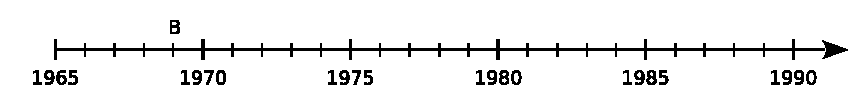
\includegraphics[width=\linewidth]{axe1965-1990}

Ce nombre est associé à un événement historique important. Lequel ?
Décalque cette demi-droite et place le point $N$ associé au nombre qui correspond à l'année de la chute du mur de Berlin.

Le nombre associé à un point sur une demi-droite graduée est l'\textbf{abscisse} de ce point.

\end{partie}

\begin{partie}[Des partages de plus en plus petits]
\begin{enumerate}
 \item Reproduis et complète la demi-droite graduée ci-dessous. \label{NbEntDec_Acti1Qa}
 
 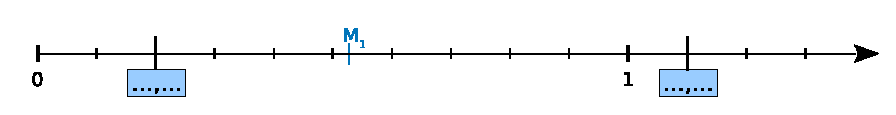
\includegraphics[width=\linewidth]{axe0-1}
 
 \item Détermine les abscisses des points $S$, $P$, $R$, $V$, $T$ et $U$ repérés en noir sur les demi-droites graduées ci-dessous.\label{NbEntDec_Acti1Qb}
 
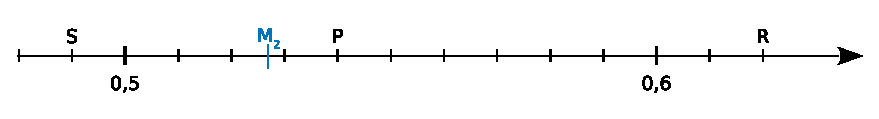
\includegraphics[width=\linewidth]{axe05-06}

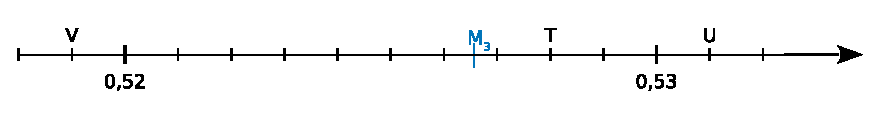
\includegraphics[width=\linewidth]{axe052-053}
 
 \item Sur une demi-droite, graduée judicieusement, place précisément les points $X$ et $Y$ d'abscisses respectives $0,526\,5$ et $0,527\,1$.
 \item Donne un \textbf{encadrement}, le plus précis possible, de l'abscisse des points $M_1$, $M_2$ et $M_3$ repérés en bleu sur les demi-droites graduées des questions \ref{NbEntDec_Acti1Qa} et \ref{NbEntDec_Acti1Qb}.
 \end{enumerate}
\end{partie}

\end{activite}


%%%%%%%%%%%%%%%%%%%%%%%%%%%%%%%%%%%%%%%%%%%%%%%%%%%%%%%%%%%%%%%%%%%%%%%%


\begin{activite}[L'écriture décimale]
\begin{enumerate}
 \item 349,785 est un nombre noté en écriture décimale. Dans ce nombre, quel est le chiffre représentant les unités ? Que désigne le chiffre 7 ? Et le chiffre 8 ?
 \item Le nombre 123,409 peut se lire « 123 virgule 409 ». Donne une autre lecture possible en utilisant les mots unités, dixièmes, centièmes et millièmes.
Que représente chacun des chiffres de ce nombre ? 4 est-il le chiffre des centaines ?
 \item Combien de centièmes y a-t-il dans un  dixième ? Dans une  unité ?
Combien de millièmes y a-t-il dans un centième ? Dans un dixième ? Dans une unité ?
 \item Combien de centièmes y a-t-il dans 7 unités 4 dixièmes ? Et dans 25 unités 8 dixièmes et 7 centièmes ?
 \end{enumerate}
\end{activite}


%%%%%%%%%%%%%%%%%%%%%%%%%%%%%%%%%%%%%%%%%%%%%%%%%%%%%%%%%%%%%%%%%%%%%%%%


\begin{activite}[Comparer, ranger et intercaler]

\begin{partie}[Comparer et ranger]
\begin{enumerate}
 \item Lequel des deux nombres 0,85 et 1,2 est le plus proche de 1 ? Quel est le nombre le plus proche de $12 : 11,9$ ou 12,08 ? Justifie avec soin tes réponses.
 \item Range les nombres de chaque liste dans l'ordre \textbf{croissant} (c'est-à-dire du plus petit au plus grand).
 	\begin{itemize}
	\item 1\,250 ; 1\,025 ; 125 ; 15\,200 ; 1\,520 ; 5\,120 ; 12\,500 ; 10\,520
	\item $10 + 0,5 + 0,06$ ; $7 + 0,5$ ; $10 + 0,06$ ; $7 + 0,05$ ; $10 + 0,6$ et $7 + 0,04 + 0,006$
	 \end{itemize}
 \item On a représenté ci-dessous une partie d'une demi-droite graduée.
 
 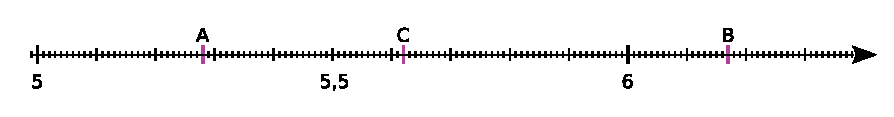
\includegraphics[width=\linewidth]{axe5A-6B}

Quelles sont les abscisses des points $A$, $B$ et $C$ ?

\vspace{0.75em}

Reproduis sur du papier millimétré cette portion de demi-droite et place les points $D$, $E$, $F$ et $G$ d'abscisses respectives 5,4 ; 6,22 ; 5,9 et 5,49.
Range alors les abscisses des points $A$, $B$, $C$, $D$, $E$, $F$ et $G$ dans l'ordre \textbf{décroissant}.
 \item À l'aide des questions précédentes et de tes connaissances, explique pourquoi les raisonnements d'élèves suivants ne sont pas justes et donne les raisons qui ont pu motiver leurs erreurs.
	\begin{itemize}
	\item \emph{« 24,5 < 6,08 car 245 < 608. »}
	\item \emph{« 19,85 < 12,96 car 0,85 < 0,96. »}
	\item \emph{« 6,012 > 6,35 car, à \textbf{partie entière} égale, le plus grand nombre est celui qui a le plus de chiffres après la virgule. »}
	\item \emph{« 5,24 > 5,8 car les parties entières sont égales et 24 > 8. »}
	\item \emph{« 14,3 < 14,30 car les parties entières sont égales et 3 < 30. »}
	\item \emph{« 103,6020 = 13,62 car les zéros ne servent à rien. »}
	\item \emph{« 16,295 < 16,38 car les parties entières sont égales et 16,295 a plus de chiffres après la virgule que 16,38. »}
	 \end{itemize}
 \end{enumerate}
\end{partie}

\begin{partie}[Intercaler]
\begin{enumerate}
 \item Quel est le nombre entier qui suit 128 ? Est-il possible de répondre à cette question si l'on remplace entier par décimal ?
Mêmes questions si on remplace 128 par 5,4.
 \item Est-il possible de trouver un nombre entier compris entre 1\,025 et 1\,026 ? Si oui, donne un exemple.
Même question en remplaçant « nombre entier » par « nombre décimal ».
 \item Est-il possible de trouver un nombre décimal compris entre 12,88 et 12,89 ? Et entre 8,975 et 8,976 ?
 \item À ton avis, est-il toujours possible de trouver plusieurs nombres décimaux compris entre deux nombres décimaux ?
 \end{enumerate}
\end{partie}

\end{activite}


%%%%%%%%%%%%%%%%%%%%%%%%%%%%%%%%%%%%%%%%%%%%%%%%%%%%%%%%%%%%%%%%%%%%%%%%

\begin{activite}[Multiplication et division par 10 ; 100 ; 1000 \ldots]

\begin{partie}[Multiplication par 10 ; 100 ; 1000 \ldots]
Le nombre 924,65 est égal à 9 centaines plus 2 dizaines plus 4 unités plus 6 dixièmes plus 5 centièmes.
\begin{enumerate}
 \item On veut multiplier par 10 le nombre suivant : 7 centaines plus 8 dizaines plus 3 unités plus 5 dixièmes plus 4 centièmes. Écris le résultat sous la même forme puis déduis-en une égalité en écriture décimale. \label{NbEntDec_Acti4Qa}
 \item Écris le nombre 15,034 comme dans la question \ref{NbEntDec_Acti4Qa}. Multiplie‑le par 1\,000 en t'inspirant de la question précédente.
 \item Donne une règle permettant de multiplier un nombre décimal par 10, 100 ou 1\,000. Que devient cette règle dans le cas d'un nombre entier ?
 \end{enumerate}
\end{partie}

\begin{partie}[Division par 10 ; 100 ; 1000 \ldots]
\begin{enumerate}
 \item En t'inspirant de la méthode précédente, divise par 10 le nombre 3 milliers plus 4 dizaines plus 6 unités plus 3 dixièmes plus 5 centièmes. Écris l'égalité en écriture décimale. \label{NbEntDec_Acti4Qa_2}
 \item Écris le nombre 73,305 comme dans la question \ref{NbEntDec_Acti4Qa_2} puis divise‑le par 1\,000.
 \item Donne une règle permettant de diviser un nombre décimal par 10, 100 ou 1\,000.
 \end{enumerate}
\end{partie}

\end{activite}


%%%%%%%%%%%%%%%%%%%%%%%%%%%%%%%%%%%%%%%%%%%%%%%%%%%%%%%%%%%%%%%%%%%%%%%%

\begin{activite}[Techniques opératoires]

\begin{partie}[Addition et soustraction de nombres décimaux]
\begin{enumerate}
 \item Pose et effectue l'opération $123,67 + 2,655$. Explique la méthode.
 \item Domitille et Virgile ont effectué cette opération et voilà ce qu'ils ont trouvé :\\[0.5em]
 
 \begin{minipage}[t]{.44\linewidth} 
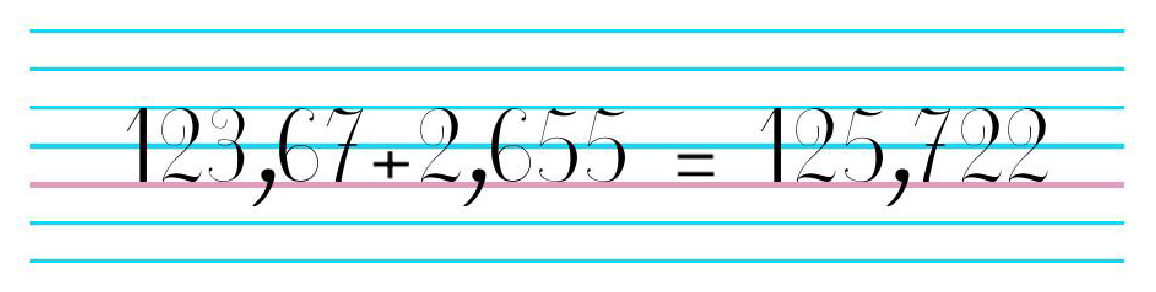
\includegraphics[width=5.5cm]{rep_domitille}
 \end{minipage}\hfill%
 \begin{minipage}[t]{.56\linewidth}
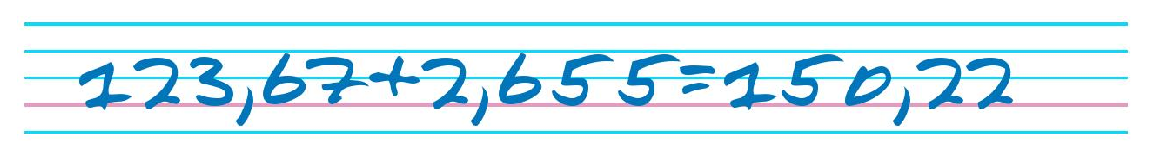
\includegraphics[width=7.5cm]{rep_virgile}
 \end{minipage}\\
  \begin{minipage}[t]{.44\linewidth} 
\begin{center} Réponse de Domitille \end{center}
 \end{minipage}\hfill%
 \begin{minipage}[t]{.56\linewidth}
\begin{center} Réponse de Virgile \end{center}
 \end{minipage}\\
 
 Que penses‑tu de leurs résultats ? Explique leurs éventuelles erreurs.
 \item Ambre était absente le jour où la maîtresse a expliqué comment on soustrait des nombres décimaux. Écris un texte le lui expliquant, donne un exemple.
 \end{enumerate}
\end{partie}

\begin{partie}[Multiplication d'un nombre décimal par un nombre entier]
\begin{enumerate}
 \item Pose et effectue l'opération $123,7 + 123,7 + 123,7 + 123,7$.
 \item Pose et effectue l'opération $123,7 \cdot 4$. Compare les deux opérations.
 \item Pose et effectue l'opération $52,8 \cdot 6$.
 \item Lucas a noté une série d'opérations pour calculer $52,8 \cdot 6$ : \\[-1em]
 
 $0,8 \cdot 6 = 4,8$ \hfill $2 \cdot 6 = 12$ \hfill $50 \cdot 6 = 300$ \hfill $300 + 12 + 4,8 = 316,8$ \\[-1em]
 
 Que penses‑tu de cette méthode ?
 \item Effectue l'opération $763,6 \cdot 3$ en utilisant la méthode de Lucas puis pose‑la pour vérifier ton résultat.
 \item Adapte cette méthode pour effectuer l'opération $1,34 \cdot 18$. Pose ensuite l'opération pour vérifier ton résultat.
 \end{enumerate}
\end{partie}

\end{activite}


%%%%%%%%%%%%%%%%%%%%%%%%%%%%%%%%%%%%%%%%%%%%%%%%%%%%%%%%%%%%%%%%%%%%%%%%



\begin{activite}[Vérifier un résultat]

\begin{enumerate}
 \item Sans poser aucune opération et sans utiliser de calculatrice, associe chaque calcul de gauche à un résultat de droite. \\[0.5em]
 
\begin{minipage}[t]{0.48\linewidth}
\begin{center}
\begin{ttableau}{0.7\linewidth}{1}
\hline \rowcolor{B3} \textbf{a.} $\quad 56 \cdot 123$ \\
\hline \rowcolor{G3} \textbf{b.} $\quad 12,35 + 1,68$ \\
\hline \rowcolor{B3} \textbf{c.} $\quad 1\,073 : 200$ \\
\hline \rowcolor{G3} \textbf{d.} $\quad 0,255 + 0,728$ \\
\hline \rowcolor{B3} \textbf{e.} $\quad 0,255 \cdot 0,728$ \\
\hline \rowcolor{G3} \textbf{f.} $\quad 13,23 : 5$ \\
\hline \rowcolor{B3} \textbf{g.} $\quad 520 \cdot 36$ \\
\hline \rowcolor{G3} \textbf{h.} $\quad 428 + 537$ \\
\hline \rowcolor{B3} \textbf{i.} $\quad 1,2 \cdot 2,4$ \\
\hline \rowcolor{G3} \textbf{j.} $\quad 18 \cdot 29$ \\
\hline
\end{ttableau}
\end{center}
\end{minipage} \hfill%
\begin{minipage}[t]{0.48\linewidth}
\begin{center}
\renewcommand*\tabularxcolumn[1]{>{\centering\arraybackslash}m{#1}}
\begin{ttableau}{0.6\linewidth}{1}
\hline \rowcolor{H3} 5,365 \\
\hline \rowcolor{J3} 2,88 \\
\hline \rowcolor{H3} 6\,888 \\
\hline \rowcolor{J3} 0,983 \\
\hline \rowcolor{H3} 2,646 \\
\hline \rowcolor{J3} 965 \\
\hline \rowcolor{H3} 522 \\
\hline \rowcolor{J3} 14,03 \\
\hline \rowcolor{H3} 18\,720 \\
\hline \rowcolor{J3} 0,185\,64 \\
\hline
\end{ttableau} 
\end{center}
 \end{minipage} \\
 
 \item Explique le plus précisément possible la manière dont tu as trouvé les résultats.\label{NbEntDec_Acti6Q2}
 \item Maverick a effectué des calculs ci-dessous. Détermine quels résultats sont forcément faux en utilisant les méthodes décrites à la question \ref{NbEntDec_Acti6Q2}.\\[1em]
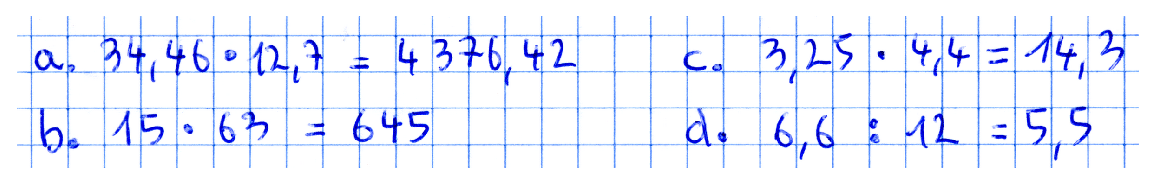
\includegraphics[width=\linewidth]{calcul_Maverick}

 \end{enumerate}
 
 \end{activite}


%%%%%%%%%%%%%%%%%%%%%%%%%%%%%%%%%%%%%%%%%%%%%%%%%%%%%%%%%%%%%%%%%%%%%%%%




\cours
\section{Le système décimal}

% remarque : pour qu'un mot se retrouve dans le lexique : \MotDefinition{asymptote horizontale}{} 

Les règles et conventions qui permettent d'écrire et de lire les nombres forment ce qu'on appelle un \textbf{système de numération}. Nous utilisons le système décimal, de base dix.

\begin{aconnaitre}
Pour écrire les chiffres dans le système décimal, il nous faut dix symboles, appelés des \emph{chiffres}. Ces chiffres sont :
\[ 0\,;\,1\,;\,2\,;\,3\,;\,4\,;\,5\,;\,6\,;\,7\,;\,8\,;\,9  \]
Il arrive parfois qu'on confonde \textbf{\MotDefinition{chiffre}{}} et \textbf{\MotDefinition{nombre}{}}. On peut faire l'analogie avec l'écriture d'une langue en affirmant que les \textbf{\textcolor{H1}{chiffres}} sont des \textbf{\textcolor{H1}{lettres}} et que les \textbf{\textcolor{H1}{nombres}} sont des \textbf{\textcolor{H1}{mots}}. Ainsi, 13 est un nombre qui s'écrit avec les chiffres 1 et 3.
\end{aconnaitre}

\newpage

\begin{methode*1}[Écriture et lecture des nombres en base 10]

L'\textbf{\textcolor{C2}{écriture décimale}} d'un nombre comporte deux parties, séparées par une virgule :

\hspace{2em}\textbullet\hspace{.25em} la partie entière, à gauche de la virgule ;

\hspace{2em}\textbullet\hspace{.25em} la partie décimale, à droite de la virgule.



Un nombre entier est caractérisé par le fait qu'il n'a pas de partie décimale (on omet alors la virgule).

\vspace{2em}

\begin{ttableau}{\linewidth}{18}
\hline
\multicolumn{3}{|c|}{milliards} & \multicolumn{3}{c|}{millions} & \multicolumn{3}{c|}{mille} & \multicolumn{3}{c|}{unités} & \multirow{2}{*}{\rotatebox{90}{dixièmes\phantom{xxx}}} & \multirow{2}{*}{\rotatebox{90}{centièmes\phantom{xxx}}} & \multirow{2}{*}{\rotatebox{90}{millièmes\phantom{xxx}}} & \multirow{2}{*}{\rotatebox{90}{dix-millièmes\phantom{xxx}}} & \multirow{2}{*}{\rotatebox{90}{centi-millièmes\phantom{xxx}}} & \multirow{2}{*}{\rotatebox{90}{millionièmes\phantom{xxx}}} \\ \cline{1-12}
\rotatebox{90}{centaines de ... } & \rotatebox{90}{dizaines de ...} & \rotatebox{90}{unités de ...} &
\rotatebox{90}{centaines de ... } & \rotatebox{90}{dizaines de ...} & \rotatebox{90}{unités de ...} &
\rotatebox{90}{centaines de ... } & \rotatebox{90}{dizaines de ...} & \rotatebox{90}{unités de ...} &
\rotatebox{90}{centaines de ... } & \rotatebox{90}{dizaines de ...} & \rotatebox{90}{unités de ...} & & & & & & \\ \hline
& & & & & & & & & & & & & & & & & \\ \hline
& & & & & 3 & 0 & 2 & 7 & 4 & 6 & 2 & 0 & 0 & 0 & 0 & 0 & 0 \\ \hline
& & & & & & & & & & 1 & 0 & 0 & 1 & & & & \\ \hline
& & & & & & & & & & & 0 & 0 & 3 & 7 & & & \\ \hline
& 2 & 0 & 0 & 0 & 0 & 0 & 4 & 2 & 0 & 0 & 0 & & & & & & \\ \hline
\end{ttableau}


\begin{exemple*1}
Le premier nombre figurant dans le tableau s'écrit 3\,027\,462.

Il se lit "trois millions vingt-sept mille quatre cent soixante-deux".

C'est un nombre entier.
\end{exemple*1}

\begin{exemple*1}
Le  deuxième nombre figurant dans le tableau s’écrit 10,01.

Il se lit "dix virgule zéro un".

Ce n’est pas un nombre entier.
\end{exemple*1}

\begin{exemple*1}
Le troisième nombre figurant dans le tableau s’écrit 0,037.

Il se lit "zéro virgule zéro trente-sept" ou "trente-sept millièmes".

Ce n’est pas un nombre entier.
\end{exemple*1}

\begin{exemple*1}
Le quatrième nombre figurant dans le tableau s’écrit 20\,000\,042\,000.

Il se lit "vingt milliards quarante-deux mille".

C’est un nombre entier.
\end{exemple*1}

\exercice 

Donne une écriture décimale du nombre cinquante-trois millions quatre cent vingt-sept mille huit cent dix-neuf virgule zéro zéro cinq cent soixante-et-un.
%\correction

\end{methode*1}

%%%%%%%%%%%%%%%%%%%%%%%%%%%%%%%%%%%%%%%%%%%%%%%%%%%%%%%%%%%%%%%%%%%%%%%%%%%

\begin{methode*1}[Repérer sur une demi-droite graduée]

\begin{aconnaitre}
Sur une demi-droite graduée, un point est repéré par un nombre appelé son \textbf{\MotDefinition{abscisse}{}}.
\end{aconnaitre}

\begin{exemple*1}

\vspace{0.5cm}

 \begin{minipage}[c]{.46\textwidth}
 Donne l'abscisse des points $A$ et $B$ puis place le point $C$ d'abscisse 4,3.
  \end{minipage}\hfill%
 \begin{minipage}[c]{.46\textwidth} 
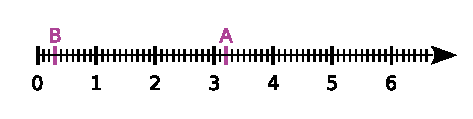
\includegraphics[width=5.5cm]{axe0BA6}
 \end{minipage}\\

Une unité est divisée en dix parts égales, ce qui signifie qu'elle est partagée en dix dixièmes. Le point $A$ se trouve 2 dixièmes à la droite du 3, donc son abscisse est $3 + 0,2 = 3,2$. De la même façon, $B$ a pour abscisse $0 + 0,3 = 0,3$. \\

  \begin{minipage}[c]{.46\textwidth}
On note $A(3,2)$ et $B(0,3)$.\\
$C(4,3) : 4,3 = 4 + 0,3$\\
$C$ se place 3 dixièmes à la droite du 4.
  \end{minipage}\hfill%
 \begin{minipage}[c]{.46\textwidth} 
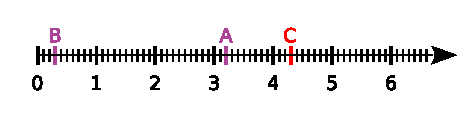
\includegraphics[width=5.5cm]{axe0BAC6}
 \end{minipage}\\

\end{exemple*1}

\exercice 

Sur une demi-droite graduée, place les points $M$ d'abscisse 2,7 et $N$ d'abscisse 5,2.
%\correction

\end{methode*1}

%%%%%%%%%%%%%%%%%%%%%%%%%%%%%%%%%%%%%%%%%%%%%%%%%%%%%%%%%%%%%%%%%%%%%%%%%%%
\begin{methode*1}[Encadrer]

\begin{aconnaitre}
\textbf{\MotDefinition{Encadrer}{}} un nombre, c'est trouver un nombre qui est plus petit que lui et un nombre qui est plus grand que lui. On écrit un encadrement avec les symboles $<$ ; $\leqslant$ ; $>$ et $\geqslant$. 
\end{aconnaitre}

\begin{exemple*1}
Encadrer 13,345 à l'unité puis au centième.\\[0.5em]
Pour encadrer à l'unité, on «coupe» le nombre 13,345 à l'unité et on obtient 13 qui est plus petit  que 13,345. Puis on ajoute \textbf{une unité}. On obtient 14 qui est plus grand que 13,345. On écrit alors : $13 < 13,345 < 14$. \\[1em]
Pour encadrer au centième, on «coupe» le nombre 13,345 au centième et on obtient 13,34 qui est plus petit que 13,345. Puis on ajoute \textbf{un centième}. On obtient 13,35 qui est plus grand que 13,345. On écrit alors : $13,34 < 13,345 < 13,35$.
\end{exemple*1}

\exercice

Encadrer les nombres 237,48 et 43,923\,5 à la dizaine puis au centième.
%\correction

\end{methode*1}

%%%%%%%%%%%%%%%%%%%%%%%%%%%%%%%%%%%%%%%%%%%%%%%%%%%%%%%%%%%%%%%%%%%%%%%%%%

\begin{methode*1}[Arrondir]

\begin{aconnaitre}
\textbf{\MotDefinition{Arrondir}{}} un nombre, c’est le remplacer par le nombre le plus proche à la précision désirée. Pour cela, on choisit le dernier chiffre à conserver puis :
\begin{itemize}
 \item on conserve ce chiffre si le suivant est 0, 1, 2, 3 ou 4 ;
 \item on augmente de 1 ce chiffre si le suivant est 5, 6, 7, 8, ou 9.
 \end{itemize}
\end{aconnaitre}

\exercice

%\correction

\end{methode*1}

%%%%%%%%%%%%%%%%%%%%%%%%%%%%%%%%%%%%%%%%%%%%%%%%%%%%%%%%%%%%%%%%%%%%%%%%%%

\section{Multiplier ou diviser}

\begin{methode*1}[Multiplier ou diviser un nombre décimal par 10 ; 100 ; 1\,000 \ldots]

\begin{aconnaitre}
\textbf{Multiplier} un nombre décimal par \textcolor{A1}{\textbf{10}}, \textcolor{B1}{\textbf{100}} ou \textcolor{J1}{\textbf{1\,000}} revient à déplacer chacun de ses chiffres vers \textbf{la gauche} de \textcolor{A1}{\textbf{1}}, \textcolor{B1}{\textbf{2}} ou \textcolor{J1}{\textbf{3}} rangs pour lui donner une valeur \textcolor{A1}{\textbf{10}}, \textcolor{B1}{\textbf{100}} ou \textcolor{J1}{\textbf{1\,000}} fois plus grande.
\textbf{Diviser} un nombre décimal par \textcolor{A1}{\textbf{10}}, \textcolor{B1}{\textbf{100}} ou \textcolor{J1}{\textbf{1\,000}} revient à déplacer chacun de ses chiffres vers \textbf{la droite} de \textcolor{A1}{\textbf{1}}, \textcolor{B1}{\textbf{2}} ou \textcolor{J1}{\textbf{3}} rangs pour lui donner une valeur  \textcolor{A1}{\textbf{10}}, \textcolor{B1}{\textbf{100}} ou \textcolor{J1}{\textbf{1\,000}} fois plus petite.
\end{aconnaitre}

\begin{remarque}
On devra parfois ajouter des zéros dans l'écriture.
\end{remarque}

\begin{exemple*1}
Effectue les calculs $6,5:100$ et $0,47 \cdot 1\,000$.\\[1em] 

\begin{minipage}{.4\linewidth}
\begin{ttableau}{.8\linewidth}{4}
\hline
 \rotatebox{90}{unités} & \rotatebox{90}{dixièmes} & \rotatebox{90}{centièmes\phantom{x}} & \rotatebox{90}{millièmes} \\ \hline
 \textcolor{B1}{\textbf{6}} , & \textcolor{B1}{\textbf{5}} & & \\ \hline
 $0\,,$ & 0 & \textcolor{B1}{\textbf{6}} & \textcolor{B1}{\textbf{5}} \\ \hline
\end{ttableau}
\end{minipage}\hfill%
%
\begin{minipage}{.55\linewidth}
Pour diviser 6,5 par \textcolor{B1}{\textbf{100}}, on déplace chacun de ses chiffres vers la droite de \textcolor{B1}{\textbf{2}} rangs et on ajoute les zéros nécessaires. 

On obtient $6,5:100 = 0,065$.

\end{minipage}
%

\vspace{2em}

%
\begin{minipage}{.4\linewidth}
\begin{ttableau}{\linewidth}{5}
\hline
\rotatebox{90}{centaines} & \rotatebox{90}{dixaines} & \rotatebox{90}{unités} & \rotatebox{90}{dixièmes} & \rotatebox{90}{centièmes\phantom{x}} \\ \hline
 & & 0 , & \textcolor{J1}{\textbf{4}} & \textcolor{J1}{\textbf{7}} \\ \hline
 \textcolor{J1}{\textbf{4}} & \textcolor{J1}{\textbf{7}} & 0 & &\\ \hline
\end{ttableau}
\end{minipage}\hfill%
%
\begin{minipage}{.55\linewidth}
Pour multiplier 0,47 par \textcolor{J1}{\textbf{1\,000}}, on déplace chacun de ses chiffres vers la gauche de \textcolor{J1}{\textbf{3}} rangs et on ajoute les zéros nécessaires. 

On obtient $0,47 \cdot 1\,000 = 470$. 
\end{minipage}
\end{exemple*1}

\exercice

Effectue : 
\begin{colenumerate}{4}
 \item $3,6 \cdot 100$ ;
 \item $870 \cdot 1\,000$ ;
 \item $63 : 10$ ;
 \item $87\,654 : 100$.
 \end{colenumerate}
%\correction
 
\exercice

Convertis en cm :
\begin{colenumerate}{4}
 \item 4 dm ;
 \item 8,1 dam ;
 \item 3,5 mm ;
 \item 0,035 m.
 \end{colenumerate}
%\correction

\end{methode*1}

%%%%%%%%%%%%%%%%%%%%%%%%%%%%%%%%%%%%%%%%%%%%%%%%%%%%%%%%%%%%%%%%%%%%%%%%%%%

\begin{methode*1}[Multiplier ou diviser un nombre décimal par 0,1 ; 0,01 ; 0,001 \ldots]

\begin{aconnaitre}
\textbf{Multiplier} un nombre décimal par \textcolor{A1}{\textbf{0,1}}, \textcolor{B1}{\textbf{0,01}} ou \textcolor{J1}{\textbf{0,001}} revient à déplacer chacun de ses chiffres vers \textbf{la droite} de 1, 2 ou \textcolor{J1}{\textbf{3}} rangs pour lui donner une valeur 10, 100 ou \textcolor{J1}{\textbf{1\,000}} fois plus petite.
\textbf{Diviser} un nombre décimal par \textcolor{A1}{\textbf{0,1}}, \textcolor{B1}{\textbf{0,01}} ou \textcolor{J1}{\textbf{0,001}} revient à déplacer chacun de ses chiffres vers \textbf{la gauche} de \textcolor{A1}{\textbf{1}}, \textcolor{B1}{\textbf{2}} ou \textcolor{J1}{\textbf{3}} rangs pour lui donner une valeur \textcolor{A1}{\textbf{10}}, \textcolor{B1}{\textbf{100}} ou \textcolor{J1}{\textbf{1\,000}} fois plus grande.
\end{aconnaitre}

\begin{remarque}
On devra parfois ajouter des zéros dans l'écriture.
\end{remarque}

\begin{exemple*1}
Effectue les calculs $2,5 \times 0,01$ et $0,65 \div 0,001$.\\[1em]

\begin{minipage}{.4\linewidth}
\begin{ttableau}{.8\linewidth}{4}
\hline
 \rotatebox{90}{unités} & \rotatebox{90}{dixièmes} & \rotatebox{90}{centièmes\phantom{x}} & \rotatebox{90}{millièmes} \\ \hline
 \textcolor{B1}{\textbf{2}} , & \textcolor{B1}{\textbf{5}} & & \\ \hline
 $0\,,$ & 0 & \textcolor{B1}{\textbf{2}} & \textcolor{B1}{\textbf{5}} \\ \hline
\end{ttableau}
\end{minipage}\hfill%
%
\begin{minipage}{.55\linewidth}
Pour multiplier 2,5 par \textcolor{B1}{\textbf{0,01}}, on déplace chacun de ses chiffres vers la droite de \textcolor{B1}{\textbf{2}} rangs et on ajoute les zéros nécessaires. 

On obtient $2,5 \times 0,01 = 0,025$.
\end{minipage}
%

\vspace{2em}

%
\begin{minipage}{.4\linewidth}
\begin{ttableau}{\linewidth}{5}
\hline
\rotatebox{90}{centaines} & \rotatebox{90}{dixaines} & \rotatebox{90}{unités} & \rotatebox{90}{dixièmes} & \rotatebox{90}{centièmes\phantom{x}} \\ \hline
 & & 0 , & \textcolor{J1}{\textbf{6}} & \textcolor{J1}{\textbf{5}} \\ \hline
 \textcolor{J1}{\textbf{6}} & \textcolor{J1}{\textbf{5}} & 0 & &\\ \hline
\end{ttableau}
\end{minipage}\hfill%
%
\begin{minipage}{.55\linewidth}
Pour diviser 0,65 par \textcolor{J1}{\textbf{0,001}}, on déplace chacun de ses chiffres vers la gauche de \textcolor{J1}{\textbf{3}} rangs et on ajoute les zéros nécessaires. 

On obtient $0,65 \div 0,001 = 650$.
\end{minipage}
\end{exemple*1}


\exercice

Effectuer :
\begin{colenumerate}{4}
 \item $5,45 \cdot 0,1$ ;
 \item $854 \cdot 0,001$ ;
 \item $63 \div 0,1$ ;
 \item $87,54 \div 0,01$.
 \end{colenumerate}
%\correction

\end{methode*1}

%%%%%%%%%%%%%%%%%%%%%%%%%%%%%%%%%%%%%%%%%%%%%%%%%%%%%%%%%%%%%%%%%%%%%%%%%%%

\begin{methode*1}[Multiplier deux nombres décimaux]

\begin{exemple*1}

Effectue la multiplication de 2,34 par 1,2.\\[1em]

On pose l'opération comme s'il s'agissait de nombres entiers. 

On effectue la multiplication de 234 par 12 sans tenir compte des virgules.

\begin{minipage}{.6\linewidth}
\begin{tabular}{rrrrcrrrr}
& 2, & 3 & 4 & $\xrightarrow{\times \text{\textcolor{B1}{\textbf{100}}}}$ & & 2 & 3 & 4 \\
$\cdot$ & & 1, & 2 & $\xrightarrow{\times \text{\textcolor{A1}{\textbf{10}}}}$ & $\cdot$ & & 1 & 2 \\ \cline{1-4} \cline{6-9}
& & & & & & 4 & 6 & 8 \\
& & & & & 2 & 3 & 4 & . \\ \cline{1-4} \cline{6-9}
2, & 8 & 0 & 8 & $\xleftarrow{\,:\,\text{\textcolor{J1}{\textbf{1\,000}}}}$ & 2 & 8 & 0 & 8 \\
\end{tabular}
\end{minipage}\hfill%
%
\begin{minipage}{.37\linewidth}
234 est \textcolor{B1}{\textbf{100}} fois plus grand que 2,34 et 12 est \textcolor{A1}{\textbf{10}} fois plus grand que 1,2. Le produit $2,34 \cdot 1,2$ est donc \textcolor{J1}{\textbf{1\,000}} fois plus petit que 2\,808. Pour obtenir le résultat, on effectue donc $2\,808 : 1\,000$.\\[0.75em]
\end{minipage}
Finalement $2,34 \cdot 1,2 = 2,808$.
\end{exemple*1}

\exercice
Sachant que $168 \cdot 32 = 5\,376$, détermine les produits (sans aucun calcul) :
\begin{colenumerate}{4}
 \item $168 \cdot 3,2$ ;
 \item $16,8 \cdot 0,32$ ;
 \item $1\,680 \cdot 3,2$ ;
 \item $1,68 \cdot 32$.
\end{colenumerate}
%\correction

\exercice

Pose et effectue les opérations :
\begin{colenumerate}{4}
 \item $68,7 \cdot 39$ ;
 \item $123 \cdot 6,3$ ;
 \item $1,3 \cdot 0,7$ ;
 \item $54,6 \cdot 8,25$.
\end{colenumerate}
%\correction

\end{methode*1}

%%%%%%%%%%%%%%%%%%%%%%%%%%%%%%%%%%%%%%%%%%%%%%%%%%%%%%%%%%%%%%%%%%%%%%%%%%%    

\begin{methode*1}[Diviser un nombre décimal par un nombre entier]

\begin{exemple*1}
Effectue la division de 75,8 par 4.\\[0.5em]

\begin{minipage}[c]{.26\textwidth}
\vspace{0em}
\begin{center}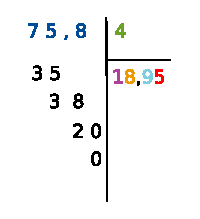
\includegraphics[width=3cm]{div758-4} \end{center}

\end{minipage}\hfill% 
\begin{minipage}[c]{.66\textwidth}

On commence par diviser la partie entière. On partage \textcolor{A1}{7} dizaines en \textcolor{H1}{4} ; le quotient comportera \textcolor{C1}{1} dizaine.\\[0.75em]
Il reste 3 dizaines. Avec les \textcolor{A1}{5} unités en plus, cela fait 35 unités à partager en \textcolor{H1}{4} ; le quotient comportera \textcolor{J1}{8} unités. \\[0.75em]
Il reste 3 unités soit 30 dixièmes. Avec les \textcolor{A1}{8} dixièmes en plus, cela fait 38 dixièmes à partager en \textcolor{H1}{4} ; le quotient comportera \textcolor{A3}{9} dixièmes. On doit donc écrire la virgule dans le quotient.\\[0.75em]
Il reste 2 dixièmes soit 20 centièmes (on a ajouté un zéro) à partager en \textcolor{H1}{4} ; le quotient comportera donc \textcolor{B2}{5} centièmes.\\[0.75em]
Ainsi $\textcolor{A1}{75,8} : \textcolor{H1}{4} = \textcolor{C1}{1}\textcolor{J1}{8},\textcolor{A3}{9}\textcolor{B2}{5}$.
\end{minipage}

\end{exemple*1}

\exercice

Calcule la valeur exacte ou une valeur arrondie au centième des quotients :
\begin{colenumerate}{4}
 \item $10 : 7$ ;
 \item $24,96 : 8$ ;
 \item $5,2 : 6$ ;
 \item $145,2 : 3$.
 \end{colenumerate}
%\correction

\end{methode*1}

%%%%%%%%%%%%%%%%%%%%%%%%%%%%%%%%%%%%%%%%%%%%%%%%%%%%%%%%%%%%%%%%%%%%%%%%%%%

\begin{methode*1}[Diviser un nombre décimal par un nombre décimal]

\begin{aconnaitre}
Le quotient de deux nombres \textbf{ne change pas} si on les multiplie (le dividende et le diviseur) par un même nombre non nul.
\end{aconnaitre}

\begin{exemple*1}
Effectue la division de 32,4 par 2,25.\\[1em]
On commence par rendre entier le diviseur en le multipliant par 100 : $2,25 \cdot 100 = 225$. On multiplie le dividende par le même nombre : $32,4 \cdot 100 = 3\,240$. On effectue la division de 3\,240  par 226, soit $3\,240 : 225 = 14,4$. On obtient ainsi le résultat de la division :

$32,4 : 2,25 = 14,4$. 
\end{exemple*1}

\exercice

Calcule la valeur exacte ou une valeur arrondie au centième des quotients :
\begin{colenumerate}{4}
 \item $4 : 6,37$ ;
 \item $13,4 : 2,45$ ;
 \item $5,87 : 2,3$ ;
 \item $0,84 : 0,12$.
 \end{colenumerate}
%\correction

\end{methode*1}

%%%%%%%%%%%%%%%%%%%%%%%%%%%%%%%%%%%%%%%%%%%%%%%%%%%%%%%%%%%%%%%%%%%%%%%%%%%        

\section{Opérations sur les durées}


%%%%%%%

\begin{methode*1}[Conversion en minutes ou en secondes]

\begin{exemple*1}

\begin{enumerate}
\item Combien y a-t-il de minutes dans 5 h 27 min ?

\begin{tabular}{ll} 
\textcolor{bleu}{\textbf{5 h}} $=$ \textcolor{bleu}{\textbf{5}} $\times$ 60 min $=$ \textcolor{bleu}{\textbf{300 min}}  & $\rightarrow$ Convertir les heures en minutes. \\
\textcolor{bleu}{\textbf{5 h}} \textcolor{vert}{\textbf{27 min}} $=$ \textcolor{bleu}{\textbf{300 min}} $+$ \textcolor{vert}{\textbf{27 min}} $=$ 327 min & $\rightarrow$ Terminer le calcul.\\
%\phantom{2 h 47 min 53 s $=$ 7\,200 s $+$ 2\,820 s $+$ 53} & \\ % phantom pour alignement avec tableau ci-dessous
\end{tabular} 

\vspace{2em}\item Combien y a-t-il de secondes dans 2 h 47 min 53 s ?

\begin{tabular}{ll} 
\textcolor{bleu}{\textbf{2 h}} $=$ \textcolor{bleu}{\textbf{2}} $\times$ 3\,600 s $=$ \textcolor{bleu}{\textbf{7\,200 s}} & $\rightarrow$ Convertir les heures en secondes. \\
\textcolor{vert}{\textbf{47 min}} $=$ \textcolor{vert}{\textbf{47}} $\times$ 60 s $=$ \textcolor{vert}{\textbf{2\,820}} s & $\rightarrow$ Convertir les minutes en secondes. \\
\textcolor{bleu}{\textbf{2 h}} \textcolor{vert}{\textbf{47 min}} 53 s $=$ \textcolor{bleu}{\textbf{7\,200 s}} $+$ \textcolor{vert}{\textbf{2\,820}} s $+$ 53 s  \\
\phantom{2 h 47 min 53 si}$=$ 10\,073 s & $\rightarrow$ Terminer le calcul. \\
\end{tabular}

\end{enumerate}
 
\end{exemple*1}

\exercice

\end{methode*1}



%%%%%%%


\begin{methode*1}[Conversion en heures, minutes et secondes]

\begin{exemple*1}
Combien y a-t-il d'heures, minutes et secondes dans 41\,000 s ? \\[1em]
\begin{minipage}[t]{.46\textwidth}
On convertit les secondes en minutes et secondes en posant la division de 41\,000 par 60 :

\begin{center}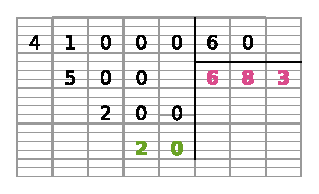
\includegraphics[width=4.6cm]{41000div60} \end{center}

On a donc 41\,000 s $=$ \textcolor{rose}{\textbf{683 min}} \textcolor{vert}{\textbf{20 s}}.
\end{minipage}\hfill%
\begin{minipage}[t]{.46\textwidth}
On convertit alors les minutes en heures et minutes en effectuant la division euclidienne de 683 par 60 :

\begin{center}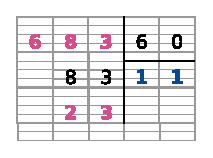
\includegraphics[width=2.9cm]{683div60} \end{center}
On a donc 41\,000 s $=$ \textcolor{bleu}{\textbf{11 h}} \textcolor{rose}{\textbf{23 min}} \textcolor{vert}{\textbf{20 s}}.
\end{minipage}


\end{exemple*1}

\exercice

\end{methode*1}

%%%%%%%%%%%%

\begin{methode*1}[Addition de durées]

\begin{exemple*1}
Un match dure 3 h 38 min et le suivant dure 2 h 49 min. Quelle est la durée totale de ces deux matchs ? \\[1em]
\begin{minipage}[t]{.34\textwidth}
On pose l'addition suivante :\\[0.2em]

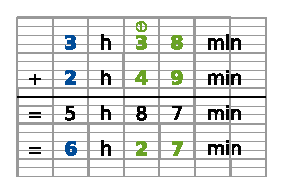
\includegraphics[width=\linewidth]{grille3h38}
\end{minipage}\hfill%
\begin{minipage}[t]{.60\textwidth}
On effectue deux additions indépendantes : 
\textcolor{vert}{\textbf{les minutes entre elles}} et \textcolor{bleu}{\textbf{les heures entre elles}}.\\[0.75em]
Mais le nombre de minutes obtenu est supérieur à 59. 
On va donc le convertir en heures et minutes sachant que 60 min $=$ 1 h. \\[0.75em]
La durée totale de ces deux matchs est donc de \textcolor{rose}{\textbf{6 h 27 min}}.
\end{minipage}

\end{exemple*1}

\exercice

Calcule :

3 h 05 min 13 s $+$ 56 min 48 s.

\vspace{1em}

1 h 46 min $+$ 2 h 37 min.

\end{methode*1}

%%%%%%%%%%%%

\begin{methode*1}[Soustraction de durées]

\begin{exemple*1}
Un film débute à 15 h 27 et finit à 18 h 14. Quelle est la durée de ce film ? \\[1em]

\begin{minipage}[t]{.34\textwidth}
On pose la soustraction suivante :\\[0.2em]

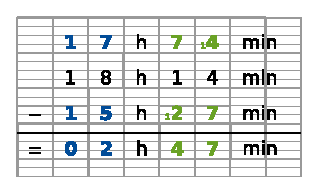
\includegraphics[width=\linewidth]{grille17h74}
\end{minipage}\hfill%
\begin{minipage}[t]{.60\textwidth}
On effectue deux soustractions indépendantes : 
\textcolor{vert}{\textbf{les minutes entre elles}} et \textcolor{bleu}{\textbf{les heures entre elles}}.\\[0.75em]
Mais on ne peut pas enlever 27 à 14. 
On va donc convertir 1 des 18 heures en 60 min. \\[0.75em]
Ce film dure donc \textcolor{rose}{\textbf{2 h 47 min}}.
\end{minipage}

\end{exemple*1}

\exercice

Calcule :

1 h 35 min 29 s $-$ 46 min 37 s.

\vspace{1em}

9 min 16 s $-$ 7 min 55 s.

%\correction

\end{methode*1}

\exercicesbase
\begin{colonne*exercice}
 \definecolor{fondTI}{HTML}{869286}


\serie{Les nombres entiers}

\begin{exercice}[Un peu de vocabulaire]
Recopie et complète les phrases suivantes afin de les rendre exactes :
\begin{enumerate}
 \item Un \ldots \ldots \ldots est composé de chiffres ;
 \item 9 est un \ldots \ldots \ldots composé d'un seul \ldots \ldots \ldots ;
 \item Le chiffre des centaines du nombre 2\,568 est \ldots \ldots ;
 \item 3 est le chiffre des \ldots \ldots \ldots du nombre 783 ;
 \item \ldots \ldots est le chiffre des milliers du nombre 120\,452 ;
 \item Le chiffre des \ldots \ldots \ldots du nombre 43 est 4.
\end{enumerate}
\end{exercice}


\begin{exercice}[« Chiffre des » ou « nombre de »]
\begin{enumerate}
 \item Recopie et complète les phrases suivantes afin de les rendre exactes :
 \begin{itemize}
  \item $127 = 12 \cdot \ldots + 7$:
  
  127 possède donc \ldots \ldots dizaines ;
  \item $841\,123 = 841 \cdot \ldots + \ldots \ldots$ :
  
  841\,123 possède donc 841 \ldots \ldots ;
  \item $3\,816 = \ldots \cdot 100 + \ldots \ldots$ :
  
  \ldots \ldots possède donc \ldots \ldots .
  \end{itemize}
 \item Dans le nombre entier 15, quel est le nombre d'unités ? Le chiffre des unités ?
 \item Combien y a-t-il de centaines dans 4\,125 ?
 \item Quel est le chiffre des dizaines dans le nombre entier 498 ? Et le nombre de dizaines ?
 \item Dans 25 dizaines, quel est le nombre d'unités ?
 \end{enumerate}
\end{exercice}


\begin{exercice}
Donne l'écriture en chiffres des nombres entiers suivants :
\begin{enumerate}
 \item $(9 \cdot 10) + 5$ ;
 \item $(7 \cdot 1\,000) + (5 \cdot 100) + (2 \cdot 10) + 8$ ;
 \item $(1 \cdot 10\,000) + (1 \cdot 100) + 1$ ;
 \item  $(3 \cdot 100\,000) + (7 \cdot 10\,000) + (4 \cdot 10) + 9$ ;
 \item  $(3 \cdot 100\,000) + (4 \cdot 100) + (7 \cdot 1\,000) + 9$.
 \end{enumerate}
\end{exercice}


\begin{exercice}
Écris en chiffres les nombres suivants :
\begin{enumerate}
 \item Sept mille huit cent douze ;
 \item Soixante-trois mille neuf cent cinquante ;
 \item Huit millions trois ;
 \item Septante-quatre milliards cent quatre ;
 \item Cent trente-six millions huit cent nonante-trois mille sept cent cinq.
 \end{enumerate}
\end{exercice}

%%%%%%%%%%%%%
\vspace{1em}%
%%%%%%%%%%%%%

\begin{exercice}
Classe les nombres suivants dans l'ordre décroissant (du plus grand au plus petit) :
\begin{colitemize}{2}
 \item 23\,100 ;
 \item Cent vingt-trois mille ;
 \item 1\,320 ;
 \item Mille cent vingt-trois.
 \end{colitemize}
\end{exercice}

%%%%%%%%%%%%%%%%%%%%%%%%%%%%%%%%%%%%%%%%%%%%%%%%%%%%%%%%%%%%%%%%%%%%%%%%%%%

\serie{Les nombres décimaux}

\begin{exercice}[Combien de \ldots dans \ldots ?]
\begin{enumerate}
 \item Combien de millièmes y a-t-il dans une unité ?
Traduis cela par une égalité mathématique.
 \item Combien de centièmes y a-t-il dans une unité ? Traduis cela par une égalité mathématique.
 \item Combien de centièmes y a-t-il dans un dixième d'unité ? Traduis cela par une égalité mathématique.
 \end{enumerate}
\end{exercice}


\begin{exercice}
Complète les égalités :
\begin{enumerate}
 \item 4 unités 6 dixièmes = \ldots \ldots dixièmes ;
 \item  \ldots \ldots  unité \ldots \ldots centièmes = 123 centièmes ;
 \item 12 unités 37 millièmes = \ldots \ldots millièmes.
 \end{enumerate}
\end{exercice}


\begin{exercice}
Donne une écriture décimale des nombres suivants :
\begin{enumerate}
 \item Sept unités et huit dixièmes \dotfill ;
 \item Cent unités, huit dixièmes et un centième
 
 \dotfill ;
 \item Deux unités et trois centièmes
 
 \dotfill ;
 \item Treize centaines \dotfill ;
 \item Trente-six milliers et huit millièmes
 
 \dotfill ;
 \item Cinq unités et quinze millièmes \dotfill.
 \end{enumerate}
\end{exercice}


\begin{exercice}[Dans un sens]
Donne l'écriture décimale :
\begin{enumerate} 
 \item 75 milliers \dotfill ; 

 \item 5 centièmes \dotfill ; 

 \item 13 dizaines \dotfill ; 

 \item 9 dixièmes \dotfill ; 

 \item 35 centaines \dotfill ;

 \item 956 millièmes \dotfill. 

 \end{enumerate}
\end{exercice}


%%%%%%%%%%%%%
\newpage    %
%%%%%%%%%%%%%


\begin{exercice}[Vocabulaire des nombres décimaux]
\begin{enumerate}
 \item Quel est le chiffre des millièmes de 24,738 ?
 
 \dotfill ;
 \item Quel est le nombre de millièmes de 24,738 ?
 
 \dotfill ;
 \item Que représente le chiffre 3 dans 7\,859,342 ?
 
 \dotfill ;
 \item Quel est le nombre de centièmes de 17,78 ?
 
 \dotfill ;
 \item Quel est le chiffre des centièmes de 71,865 ?
 
 \dotfill ;
 \item Donne la partie entière du nombre 83,712 :
 
 \dotfill ;
 \item Donne la partie décimale du nombre 54,91 :
 
 \dotfill.
 \end{enumerate}
\end{exercice}


\begin{exercice}
Trouve un nombre à cinq chiffres ayant 7 pour chiffre des dizaines, 9 pour chiffre des centièmes, 0 pour chiffre des unités, 3 pour chiffre des millièmes et comme autre chiffre 1.
\end{exercice}


\begin{exercice}[Devinette]
Trouve le nombre ayant les caractéristiques suivantes :
\begin{itemize}
 \item il n'a que deux chiffres après la virgule ;
 \item il a la même partie entière que 1 890,893 ;
 \item son chiffre des centièmes est le même que celui de 320,815 ;
 \item son chiffre des dixièmes est égal à la moitié de celui de 798,635.
 \end{itemize}
\end{exercice}


\begin{exercice}[Zéros inutiles]
Écris, lorsque cela est possible, les nombres suivants avec moins de chiffres.
\begin{enumerate} 
 \item 17,200 \dotfill ; 
 
 \item 123,201 \dotfill ; 
  
 \item 36,700\,10 \dotfill ; 
 
 \item 0\,021,125 \dotfill ; 
 
 \item 0,123\,0 \dotfill ; 
 
 \item 023,201\,20 \dotfill ; 
 
 \item 30,000 \dotfill ; 
 
 \item 0\,050,12 \dotfill ; 
 
 \item 1\,205\,500,0 \dotfill. 
  
 \end{enumerate}
\end{exercice}


%%%%%%%%%%%%%
\vspace{2em}%
%%%%%%%%%%%%%


\begin{exercice}[Décomposition]
Donne une écriture décimale qui correspond à chacune des décompositions suivantes :
\begin{enumerate}
 \item $(3 \cdot 10) + (4 \cdot 1) + (4 \cdot 0,1) + (7 \cdot 0,01)$
 \item $(8 \cdot 100) + (5 \cdot 1) + (9 \cdot 0,1) + (6 \cdot 0,01)$
 \item $(5 \cdot 1) + (4 \cdot 0,01) + (3 \cdot 0,001)$
 \item $(7 \cdot 100) + (9 \cdot 1) + (8 \cdot 0,1) + (6 \cdot 0,001)$
 \end{enumerate}
\end{exercice}


\begin{exercice}[Décomposition (bis)]
Décompose chacun de ces nombres de la même façon qu'à l'exercice précédent :
\begin{enumerate} 
 \item 9,6 \dotfill ; 
 
 \item 84,258 \dotfill ; 
 
 \item 7,102 \dotfill ;
 
 \item 123,015 \dotfill ; 
 
 \item 0,008\,3 \dotfill ; 
 
 \item 1\,002,200\,4 \dotfill.
 
 \end{enumerate}
\end{exercice}

\begin{exercice}[Sur une demi-droite graduée]
Donne les abscisses des points $A$, $B$ et $C$, sous la forme d'un nombre décimal.
\begin{center} 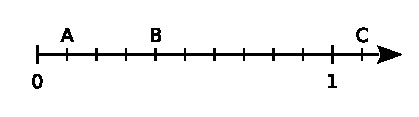
\includegraphics[width=7cm]{axe0AB1C} \end{center}
\end{exercice}


\begin{exercice}
Sur la demi-droite graduée ci-dessous, place les points $O(0)$, $A(1)$, $B(2)$, $C(0,5)$, $D(1,6)$, $E(0,1 + 0,05)$, $F(0,2)$, $G(1 + 0,05)$ et $H(1,45)$ :
\begin{center} 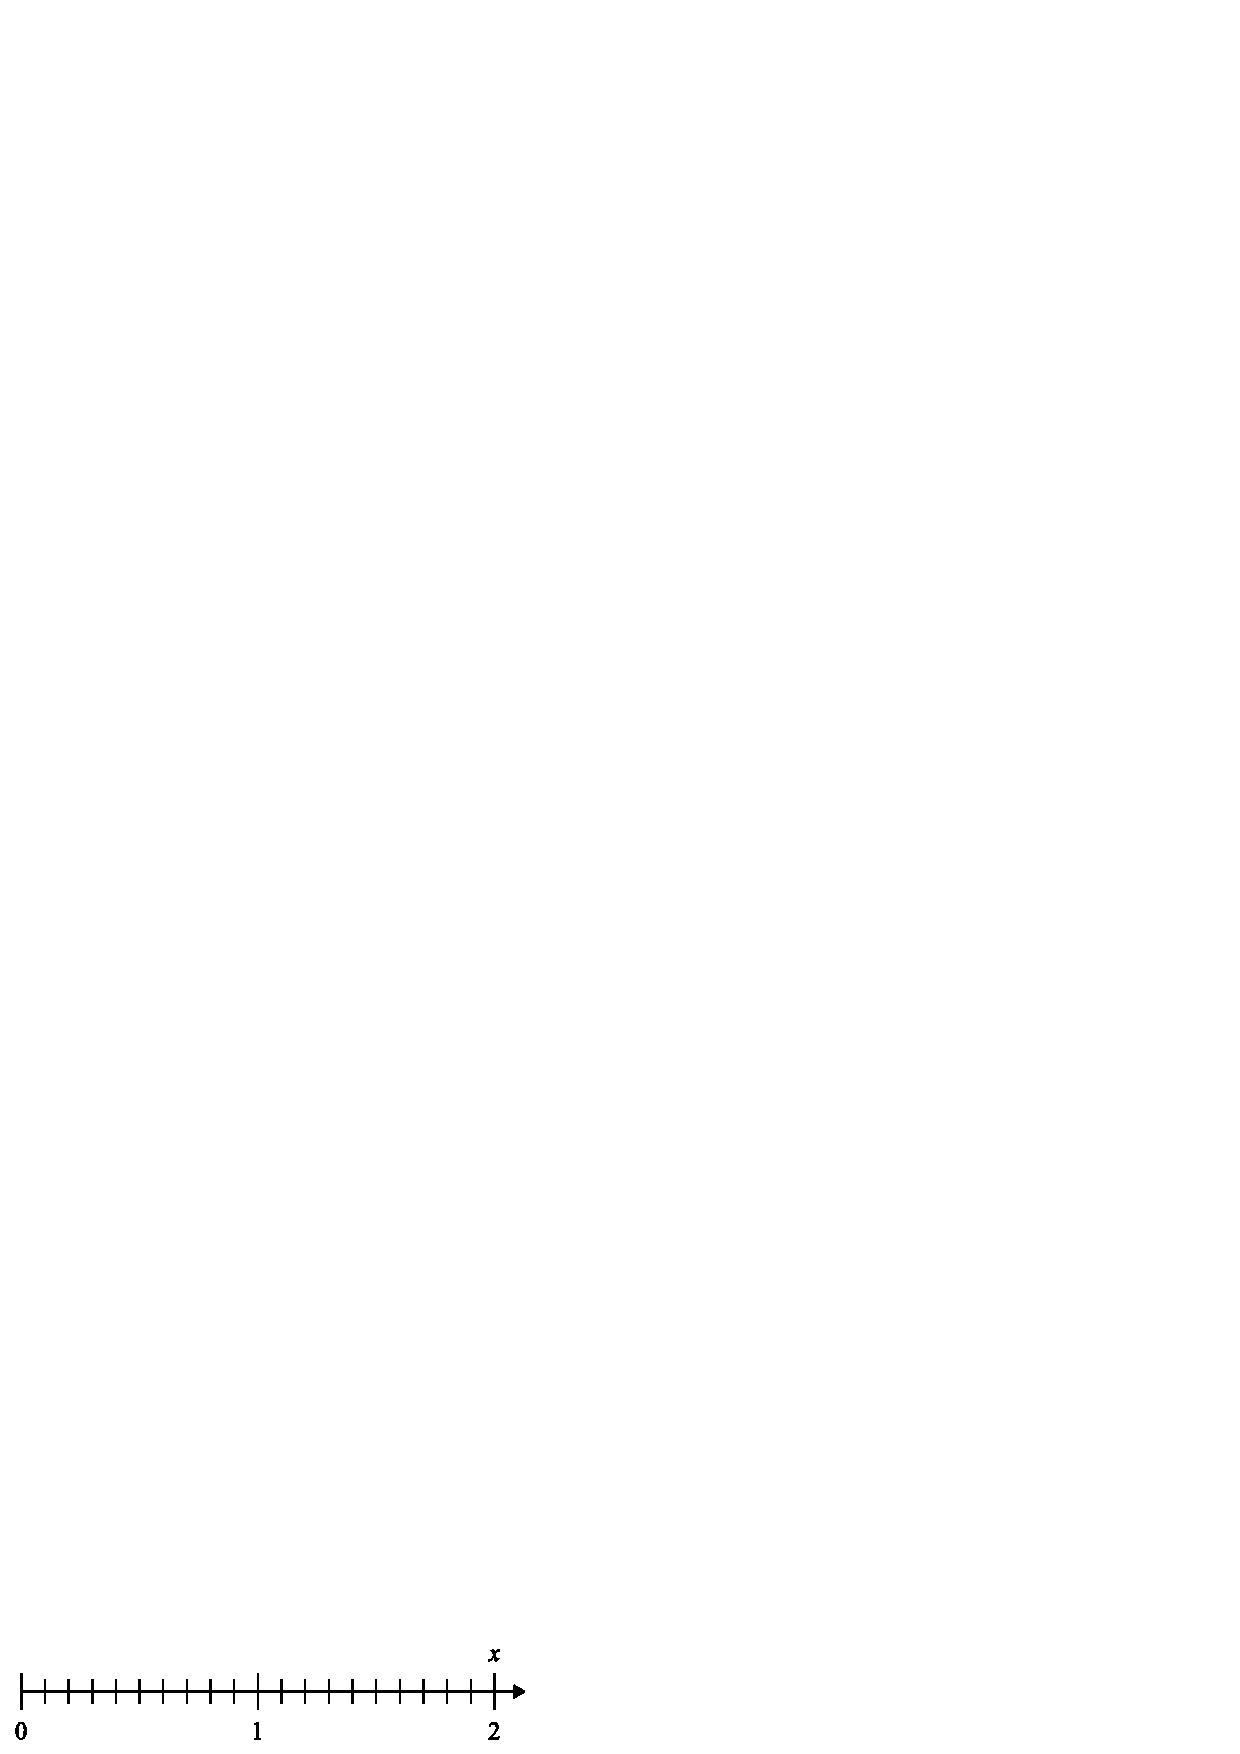
\includegraphics[width=7cm]{axe012x} \end{center}
\end{exercice}

%%%%%%%%%%%%%%%%%%%%%%%%%%%%%%%%%%%%%%%%%%%%%%%%%%%%%%%%%%%%%%%%%%%%%%%%%%%

\serie{Comparaison}

\begin{exercice}[Demi-droite graduée et comparaison]
\begin{enumerate}
 \item Reproduis la demi-droite graduée suivante et place les points $A(7,39)$ ; $B(7,46)$ et $C(7,425)$ :
\begin{center} 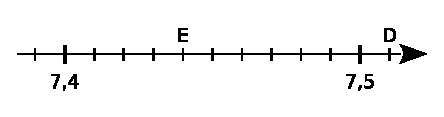
\includegraphics[width=6.6cm]{axe74E-75D} \end{center}
 \item Range dans l'ordre décroissant les abscisses de tous les points qui sont nommés.
 \end{enumerate}
\end{exercice}



%%%%%%%%%%%%%
\newpage    %
%%%%%%%%%%%%%



\begin{exercice}[Rangement]
Range les nombres suivants dans l'ordre croissant :

5 ; 4,99 ; 4,9 ; 4,88 ; 5,000 1 ; 4,909 ; 4,879 :

\dotfill

\dotfill
\end{exercice}


\begin{exercice}[Rangement $(bis)$]
Range les nombres suivants dans l'ordre décroissant :

120 ; 119,999 ; 120,000 1 ; 120,101 ; 119,9 ; 119 ; 119,990 9 ; 120,100 1 ; 102,01 ; 120,1 :

\dotfill

\dotfill
\end{exercice}

%%%%%%%%%%%%%%%%%%%%%%%%%%%%%%%%%%%%%%%%%%%%%%%%%%%%%%%%%%%%%%%%%%%%%%%%%%%

\serie{Arrondir}

\begin{exercice}[Arrondir à l'unité]
Arrondis à l'unité les nombres suivants :
\begin{enumerate}
 \item 46,8 \dotfill ; 
 
 \item 109,75 \dotfill ; 
 
 \item 1,3 \dotfill ; 
 
 \item 0,09 \dotfill ; 
 
 \item 234,08 \dotfill ; 
 
 \item 4\,087,63 \dotfill. 
 
 \end{enumerate}
\end{exercice}


\begin{exercice}[Arrondir à la dizaine]
Arrondis à la dizaine les nombres suivants :
\begin{enumerate}
 \item 234,2 \dotfill ; 
 
 \item 3,14 \dotfill ; 
 
 \item 17,62 \dotfill ; 
 
 \item 889,3 \dotfill ; 
 
 \item 6\,289,3 \dotfill ; 
 
 \item 23,005 \dotfill. 
 
 \end{enumerate}
\end{exercice}


\begin{exercice}[Arrondir au dixième]
Arrondis au dixième les nombres suivants :
\begin{enumerate}
 \item 8,372 \dotfill ; 
 
 \item 50,64 \dotfill ; 
 
 \item 30,18 \dotfill ; 
 
 \item 43,725 \dotfill ; 
 
 \item 0,02 \dotfill ; 
 
 \item 78,66 \dotfill. 
 
 \end{enumerate}
\end{exercice}


%%%%%%%%%%%%%%%%%%%%%%%%%%%%%%%%%%%%%%%%%%%%%%%%%%%%%%%%%%%%%%%%%%%%%%%%%%%



%%%%%%%%%%%%%
\vspace{6em}%
%%%%%%%%%%%%%


\serie{Encadrer}


\begin{exercice}[Encadrer à la dizaine]
235,5 ; 45 ; 1270 ; 574,23 ; 10\,095.
\end{exercice}


\begin{exercice}[Encadrer au dixième]
76,123 ; 461,99 ; 1\,254,01 ; 3,93 ; 9,99.
\end{exercice}



\begin{exercice}
Dans chaque cas, propose, si cela est possible, un nombre entier que l'on peut intercaler entre les deux nombres donnés. 
Y a‑t‑il plusieurs solutions ? Si oui, cite‑les :
\begin{enumerate}
 \item $5 < …… < 6$ ;
 \item $6,4 < …… < 6,8$ ;
 \item $3,8 < …… < 5,3$ ;
 \item $6,5 < …… < 7,21$.
 \end{enumerate}
\end{exercice}


\begin{exercice}
Dans chaque cas, donne trois exemples différents de nombres décimaux que l'on peut intercaler entre les deux nombres donnés :
\begin{enumerate}
 \item $6 < …… < 7$ ;
 \item $4,5 < …… < 4,9$ ;
 \item $3,45 < …… < 3,48$ ;
 \item $6,8 < …… < 6,9$ ;
 \item $15,13 < …… < 15,14$ ;
 \item $3,238 < …… < 3,24$.
 \end{enumerate}
\end{exercice}


\begin{exercice}[Chiffres masqués]
Certains chiffres sont masqués par \#. Lorsque cela est possible, complète les pointillés avec $<$,$>$ ou $=$ :
\begin{enumerate} 
 \item $6,51 …… 6,7\#$ ;
 \item $5,42 …… 5,0\#$ ;
 \item $\#,23 …… 4,16$ ;
 \item $6,04 …… 6,1\#$ ;
 \item $3,\#35 …… 3,01$ ;
 \item $43,\#96 …… 43,0\#$.
 \end{enumerate}
\end{exercice}


\begin{exercice}[Nombres à trouver]
Dans chaque cas, complète les pointillés par un nombre décimal :
\begin{enumerate} 
 \item $24,5 < ...... < 24,6$ ;  
 
 \item $12,99 < ...... < 13$ ; 
 
 \item $32,53 < ...... < 32,54$ ; 
 
 \item $58 < ...... < 58,01$ ; 
 
 \item $5,879 < ...... < ...... < ...... < 5,88$. 

 \end{enumerate}
\end{exercice}

%%%%%%%%%%%%%%%%%%%%%%%%%%%%%%%%%%%%%%%%%%%%%%%%%%%%%%%%%%%%%%%%%%%%%%%%%%%



%%%%%%%%%%%%%
\newpage    %
%%%%%%%%%%%%%



\serie{Techniques opératoires}


\begin{exercice}
Calcule mentalement les additions :
\begin{enumerate} 
 \item $4,6 + 5,2$ \dotfill ; 
 
 \item $6,2 + 3,4$ \dotfill ; 
 
 \item $4,5 + 6,1$ \dotfill ; 
 
 \item $8,3 + 9,6$ \dotfill ; 
 
 \item $8 + 1,5$ \dotfill ; 
 
 \item $8,6 + 8,9$ \dotfill ; 
 
 \item $3,9 + 5,4$ \dotfill ; 
 
 \item $6,5 + 8,7$ \dotfill ; 
 
 \item $6,8 + 9,4$ \dotfill ; 
 
 \item \hspace{0.1em} $12,9 + 15,8$ \dotfill. 

 \end{enumerate}
\end{exercice}


\begin{exercice}
Calcule mentalement les soustractions :
\begin{enumerate} 
 \item $6,5 - 4,3$ \dotfill ; 
 
 \item $7,6 - 0,4$ \dotfill ; 
 
 \item $4,9 - 4,3$ \dotfill ; 
 
 \item $5,7 - 0,4$ \dotfill ; 
 
 \item $4,7 - 4,3$ \dotfill ; 
 
 \item $6,2 - 4,6$ \dotfill ; 
 
 \item $9 - 8,7$ \dotfill ; 
 
 \item $3,1 - 1,8$ \dotfill ; 
 
 \item $7,8 - 6,9$ \dotfill ; 
 
 \item \hspace{0.2em}$17,4 - 8,7$ \dotfill. 
 
 \end{enumerate}  
\end{exercice}


\begin{exercice}
Calcule les sommes en effectuant des regroupements astucieux :
\begin{enumerate} 
 \item $6,5 + 12,6 + 1,5$ ;
 \item $36,99 + 45,74 + 2,01 + 13,26$ ;
 \item $9,25 + 8,7 + 5,3 + 16,75$ ;
 \item $34,645 + 34,75 + 2,25 + 4,355$ ;
 \item $7,42 + 4,2 + 7,8 + 25,58$ ;
 \item $3,01 + 2,9 + 6,1 + 7,99 + 2,001$.
 \end{enumerate}
\end{exercice}


\begin{exercice}
Pose et effectue :
\begin{enumerate} 
 \item $853,26 + 4 038,3$ ;
 \item $52 + 8,63 + 142,8$ ;
 \item $49,3 + 7,432 + 12,7$ ;
 \item $948,25 - 73,2$ ;
 \item $9,8 - 0,073$ ;
 \item $83 - 43,51$.
 \end{enumerate} 
 \end{exercice}


\begin{exercice}
Calcule mentalement :
\begin{enumerate} 
 \item $4,357 \cdot 100$ \dotfill ; 
 
 \item $89,7 \cdot 1\,000$ \dotfill ; 
 
 \item $0,043 \cdot 10$ \dotfill ; 
 
 \item $0,28 \cdot 1\,000$ \dotfill ; 
 
 \item $39 \cdot 100$ \dotfill ; 
 
 \item $0,48 \cdot 10$ \dotfill ; 
 	
 \item $354 \cdot 10$ \dotfill ; 
 	
 \item $0,03 \cdot 10\,000$ \dotfill ; 
 
 \end{enumerate}
\end{exercice}


\begin{exercice}
Calcule mentalement :
\begin{enumerate} 
 \item $4\,338 : 10$ \dotfill ; 
 
 \item $1\,297 : 1\,000$ \dotfill ; 
 	
 \item $12,3 : 10$ \dotfill ; 
 
 \item $0,87 : 100$ \dotfill ; 
 	
 \item $3,8 : 1\,000$ \dotfill ; 
 
 \item $0,04 : 100$ \dotfill ; 
 	
 \item $354 : 10$ \dotfill ; 
 
 \item $12,5 : 100$ \dotfill. 
 
 \end{enumerate}
\end{exercice}


\begin{exercice}
Calcule mentalement :
\begin{enumerate} 
 \item $435,7 \cdot 0,1$ \dotfill ; 
 
 \item $18,73 \cdot 0,01$ \dotfill ; 
 
 \item $439,345 \cdot 0,001$ \dotfill ; 
 
 \item $0,28 \cdot 0,1$ \dotfill ; 
 
 \item $39 \cdot 0,001$ \dotfill ; 
 
 \item $0,8 \cdot 0,01$ \dotfill ; 
 
 \item $354 \cdot 0,001$ \dotfill ; 
 
 \item $0,03 \cdot 0,001$ \dotfill. 
 
 \end{enumerate}
\end{exercice}

\begin{exercice}
Calcule mentalement :
\begin{enumerate} 
 \item $48 \div 0,1$ \dotfill ; 
 
 \item $12,97 \div 0,01$ \dotfill ; 

 \item $12,3 \div 0,001$ \dotfill ; 
 
 \item $0,45 \div 0,1$ \dotfill ; 
 	
 \item $5,61 \div 0,0001$ \dotfill ; 
 	
 \item $0,056 \div 0,1$ \dotfill ; 
 
 \item $354 \div 0,001$ \dotfill ; 
 
 \item $0,5 \div 0,001$ \dotfill. 

 \end{enumerate}
\end{exercice}


\begin{exercice}
Complète par 10 ; 100 ; 1\,000 ; 10\,000 \ldots :
\begin{enumerate} 
 \item $8,79 \cdot \dotfill = 87,9$ ; 
 
 \item $4,35 \cdot \dotfill = 43\,500$ ; 
 
 \item $0,837 \cdot \dotfill = 8,37$ ; 
 
 \item $0,367 \cdot \dotfill = 3,67$ ; 
 
 \item $0,028 \cdot \dotfill = 0,28$ ; 
 
 \item $0,17 \div \dotfill = 0,017$ ; 
 
 \item $23 \div \dotfill = 0,23$ ; 
 
 \item $480 \div \dotfill = 4,8$ ; 
 
 \item $900 \div \dotfill = 0,09$ ; 
 
 \item \hspace{0.25em}$18\,000 \div \dotfill = 18$. 
 
 \end{enumerate}
\end{exercice}


\begin{exercice}
Complète par le signe opératoire qui convient :
\begin{colenumerate}{2}
 \item $0,8 \ldots 100 = 80$ ;
 \item $0,38 \ldots 10 = 0,038$ ;
 \item $47 \ldots 100 = 0,47$ ;
 \item $380 \ldots 10 = 38$ ;
 \item $5 \ldots 0,1 = 0,5$ ;
 \item $60\,000 \ldots 10 = 6\,000$ ;
 \item $4\,100 \ldots 100 = 4\,000$ ;
 \item $5\,600 \ldots 100 = 56$ ;
 \item $8 \ldots 0,01 = 0,08$ ;
 \item \hspace{0.25em}$100 \ldots 1,2 = 120$.
 \end{colenumerate} 
\end{exercice}


\begin{exercice}
Calcule mentalement en détaillant ta démarche :
\begin{enumerate} 
 \item $0,1 \cdot 14 \cdot 1\,000$ \dotfill ; 
 
 \item $2,18 \cdot 0,001 \cdot 100$ \dotfill ; 

 \item $1,8 \cdot 0,01 \cdot 10$ \dotfill ; 

 \item $4 •\cdot 0,01 \cdot 100$ \dotfill. 

 \end{enumerate} 
\end{exercice}


\begin{exercice}
Sachant que $48 \cdot 152 = 7\,296$, détermine les résultats des calculs :
\begin{enumerate} 
 \item $48 \cdot 1,52$ \dotfill ; 
 
 \item $4,8 \cdot 15,2$ \dotfill ; 
 
 \item $0,48 \cdot 0,152$ \dotfill ; 
 
 \item $0,048 \cdot 1\,520$ \dotfill. 

 \end{enumerate} 
\end{exercice}


\begin{exercice}
Calcule en regroupant astucieusement :
\begin{enumerate} 
 \item $0,8 \cdot 2 \cdot 0,6 \cdot 50$ \dotfill ; 
 
 \item $0,25 \cdot 12,38 \cdot 4$ \dotfill ; 
 
 \item $8 \cdot 49 \cdot 1,25$ \dotfill ; 
 
 \item $2,5 \cdot 12,9 \cdot 0,04$ \dotfill ; 
 
 \item $0,15 \cdot 70 \cdot 0,02$ \dotfill ; 
 
 \item $75 \cdot 0,06 \cdot 0,4$ \dotfill. 
 
 \end{enumerate} 
\end{exercice}


\begin{exercice}
Place correctement la virgule dans le résultat de la multiplication (en ajoutant éventuellement un ou des zéros) :
\begin{enumerate} 
 \item $12,8 \cdot  5,3 = \textcolor{PartieGeometrie}{6\,784}$ ;
 \item $28,7 \cdot 1,04 = \textcolor{PartieGeometrie}{29\,848}$ ;
 \item $0,15 \cdot 6,3 = \textcolor{PartieGeometrie}{945}$ ;
 \item $0,008 \cdot 543,9 = \textcolor{PartieGeometrie}{43\,512}$ ;
 \item $0,235 \cdot 0,132 = \textcolor{PartieGeometrie}{3\,102}$.
 \end{enumerate}
\end{exercice}


\begin{exercice}
Place la virgule dans le nombre écrit en \textcolor{BleuOuv}{bleu} pour que l'égalité soit vraie :
\begin{enumerate} 
 \item $3,42 \cdot \textcolor{BleuOuv}{271} = 9,268\,2$ ;
 \item $\textcolor{BleuOuv}{432} \cdot 0,614 = 26,524\,8$ ;
 \item $0,48 \cdot \textcolor{BleuOuv}{62} = 29,76$ ;
 \item $2,6 \cdot \textcolor{BleuOuv}{485} = 126,1$ ;
 \item $\textcolor{BleuOuv}{45} \cdot 29,232 = 131,544$.
 \end{enumerate}
\end{exercice}

\begin{exercice}
Pose et effectue les produits :
\begin{enumerate} 
 \item $2,08 \cdot 4,23$ \dotfill ; 
 
 \item $4,38 \cdot 5,7$ \dotfill ; 
 
 \item $6,93 \cdot 15,8$ \dotfill ; 
 
 \item $8,35 \cdot 0,18 $\dotfill.  
 \end{enumerate}
\end{exercice}


\begin{exercice} 
Calcule mentalement :
\begin{colenumerate}{2}
 \item $ 8,6 \div 2$ ;
 \item $ 24,8 \div 4$ ;
 \item $ 8,8 \div 8$ ;
 \item $ 7,7 \div 11$ ;
 \item $ 15,6 \div 3$ ;
 \item $ 63,6 \div 6$.
 \end{colenumerate}
\end{exercice}


\begin{exercice} 
Pose et effectue les divisions suivantes pour en trouver le quotient décimal exact :
\begin{enumerate} 
 \item $ 12,6 \div 6$ \dotfill ; 
 
 \item $ 28,48 \div 4$ \dotfill ; 

 \item $ 169,2 \div 3$ \dotfill ; 

 \item $ 0,162 \div 9$ \dotfill ; 

 \item $ 67,5 \div 4$ \dotfill ; 

 \item $ 9,765 \div 15$ \dotfill. 
 \end{enumerate}
\end{exercice}

\begin{exercice}[Valeurs approchées]
\vspace{-1em}
\begin{enumerate} 
 \item Pose et effectue les divisions suivantes jusqu'au millième :
 \begin{itemize}
  \item $12 \div 7$ \dotfill ; 
  
  \item $148,9 \div 12$ \dotfill ; 
  
  \item $13,53 \div 3$ \dotfill. 
  \end{itemize}
 \item Pose et effectue les divisions suivantes jusqu'au centième :
  \begin{itemize}
  \item $123,8 \div 7$ \dotfill ; 
  
  \item $235,19 \div 11$ \dotfill ; 
  
  \item $0,14 \div 3$ \dotfill. 
  \end{itemize}
 \end{enumerate}
\end{exercice}


\begin{exercice} 
Calcule la valeur exacte ou une valeur arrondie au centième des divisions suivantes :
\begin{enumerate} 
 \item $1 \div 2,74$ \dotfill ; 

 \item $5,87 \div 2,3$ \dotfill ; 

 \item $3,24 \div 1,7$ \dotfill ; 

 \item $45,6 \div 0,24$ \dotfill ; 

 \item $20,35 \div 8,5$ \dotfill ; 

 \item $0,53 \div 0,17$ \dotfill. 
 \end{enumerate}
\end{exercice}


\begin{exercice} 
Calcule la valeur exacte ou une valeur arrondie au centième des divisions suivantes :
\begin{enumerate} 
 \item $3,35 \div 0,42$ \dotfill ; 

 \item $41,5 \div 3,14$ \dotfill ; 

 \item $ 0,03 \div 2,1$ \dotfill ; 

 \item $0,35 \div 0,25$ \dotfill ; 

 \item $0,53 \div 0,8$ \dotfill ; 

 \item $21,7 \div 0,14$ \dotfill. 
 \end{enumerate}
\end{exercice}

%%%%%%%%%%%%%%%%%%%%%%%%%%%%%%%%%%%%%%%%%%%%%%%%%%%%%%%%%%%%%%%%%%%%%%%%%%%

\serie{Heures, minutes, secondes}



\begin{exercice}
Convertis en heures et minutes :\\
78 min ; 134 min ; 375 min ; 35 min ; 3\,840 s.
\end{exercice}


\begin{exercice}
Effectue les calculs :
\begin{enumerate} 
 \item 3 h 25 min $+$ 5 h 33 min ;
 \item 12 h 28 min $-$ 9 h 17 min ;
 \item 6 h 38 min $+$ 19 h 53 min ;
 \item 21 h 15 min $-$ 9 h 29 min ;
 \item 5 h 13 min 33 s $+$ 9 h 45 min 47 s ;
 \item 9 h 6 min 15 s $-$ 8 h 39 min 36 s.
 \end{enumerate}
\end{exercice}


\begin{exercice}
Pose et effectue les opérations suivantes :
\begin{enumerate} 
 \item 18 h 15 min 22 s $+$ 9 h 37 min 43 s ;
 \item 12 h 26 min 52 s $-$ 7 h 39 min 57 s ;
 \item 9 h 38 min 22 s $+$ 4 h 59 min 34 s ;
 \item 12 h 40 min 21 s $-$ 6 h 35 s.
 \end{enumerate}
\end{exercice}


\begin{exercice}
Pose et effectue les opérations suivantes :
\begin{enumerate} 
 \item 13 h 25 min 42 s $+$ 12 h 35 min 52 s ;
 \item 15 h 43 min 08 s $-$ 6 h 51 min 34 s ;
 \item 10 h 41 s $+$ 9 h 57 min 49 s ;
 \item 21 h $-$ 17 h 31 min 32 s.
 \end{enumerate}
\end{exercice}


\begin{exercice}
Un randonneur part en promenade à 9 h 30. Il rentre à 12 h 05, ne s'étant arrêté pour se reposer que lors de trois pauses de 5 min chacune. Pendant combien de temps ce randonneur a‑t‑il marché ?
\end{exercice}


\begin{exercice}
Pierre part de chez lui à 9 h 55 pour aller faire des courses. Il met 12 min pour se rendre au supermarché et il y reste pendant 1 h 35 min.
\begin{enumerate} 
 \item À quelle heure repart‑il du supermarché ?
 \item Il rentre ensuite chez lui et y arrive à 12 h 01. Combien de temps son trajet de retour a‑t‑il duré ?
 \end{enumerate}
\end{exercice}


\begin{exercice}
Sarah a noté les heures de lever et de coucher du Soleil en septembre 2008. Le $1^{er}$ septembre, le Soleil s'est levé à 7 h 09 et il s'est couché à 20 h 31. Le 30 septembre, le Soleil s'est levé à 7 h 50 et il s'est couché à 19 h 30. De quelle durée les jours ont‑ils diminué au mois de septembre 2008 ?
\end{exercice}
 

\end{colonne*exercice}


\exercicesappr
\begin{colonne*exercice}
\begin{exercice}
Antoine possédait 832,25 CHF sur son livret d'épargne. Pour son anniversaire, ses parents y ont déposé 75 CHF. Combien a-t-il maintenant sur son livret ?
\end{exercice}


\begin{exercice}
Un panier plein de fruits pèse 1,836 kg. Vide, il pesait 0,425 kg. Quelle est la masse des fruits contenus dans ce panier ?
\end{exercice}


\begin{exercice}
Pierre a relevé le compteur de sa voiture au départ et au retour de vacances. Au départ, le compteur indiquait 58\,257,6 km. Au retour, il indiquait 59\,329,1 km. Quelle distance a‑t‑il parcourue pendant ses vacances ?
\end{exercice}


\begin{exercice}
Simon veut acheter un livre. Il a 25,35 CHF dans son porte‑monnaie et il lui manque 5,25 CHF pour acheter ce livre. Quel est le prix du livre ?
\end{exercice}


\begin{exercice}
Une voiture consomme 8,5 l d'essence pour faire 100 km. Combien d'essence consomme‑t‑elle pour faire 500 km ?
\end{exercice}
  
  
\begin{exercice}
Un employé gagne 17,25 CHF de l'heure. Il travaille 35 heures par semaine. Combien gagne‑t‑il chaque semaine ?
\end{exercice}


\begin{exercice}
Au marché, Anne a déposé dans son panier 1,2 kg de carottes, 600 g de raisin et 1,3 kg de pommes. Combien pèse le contenu de son panier ?
\end{exercice}


\begin{exercice}
Pour aller au collège, Caroline fait 1,4 km avec son vélo qu'elle laisse chez sa grand‑mère. Puis elle parcourt 150 m à pied jusqu'au collège. Quelle distance totale parcourt‑elle pour se rendre au collège ?
\end{exercice}


\begin{exercice}
Djamel a acheté 1,6 kg de poires à 2,30 CHF le kg. Combien a‑t‑il payé ?
\end{exercice}


\begin{exercice}
Gérard a payé 41,40 CHF pour 12 pieds de tomate. Quel est le prix d'un pied de tomate ?
\end{exercice}



\begin{exercice}
Un lot de six stylos identiques coûte 8,10 CHF. Quel est le prix d'un stylo ?
\end{exercice}


\begin{exercice}
Mercredi après‑midi, Anh Hao a fait cinq tours d'un circuit de VTT. Il a parcouru en tout 23,5 km. Quelle est la longueur de ce circuit ?
\end{exercice}


\begin{exercice}
Mme Betty possède 6,6 litres de jus de pomme. Combien de bouteilles de 0,7 litres pourra-t-elle remplir ?
\end{exercice}

\begin{exercice}
Agan possède 37,40 CHF en pièces de 20 centimes. Combien de pièces de 20 centimes possède t'il ?
\end{exercice}


\begin{exercice}[Énigme]
Trouve le nombre décimal à six chiffres tel que :
\begin{itemize}
 \item son chiffre des unités est 2 ;
 \item l'un de ses chiffres est 6 et sa valeur dans l'écriture décimale est cent fois plus petite que celle du chiffre 2 ;
 \item son chiffre des dizaines est le double de celui des unités et son chiffre des dixièmes est le quart de celui des dizaines ;
 \item ce nombre est compris entre 8\,975,06 et 9\,824,95 ;
 \item la somme de tous ses chiffres est égale à 27.
 \end{itemize}
\end{exercice}



\begin{exercice}[Nombres croisés]
Recopie et complète la grille à l'aide des nombres que tu trouveras grâce aux définitions :

\begin{center}
\begin{tabularx}{.5\linewidth}{r|c|c|c|c|c|}
\multicolumn{1}{c}{}& \multicolumn{1}{c}{\textbf{A}} & \multicolumn{1}{c}{\textbf{B}} & \multicolumn{1}{c}{\textbf{C}} & \multicolumn{1}{c}{\textbf{D}} & \multicolumn{1}{c}{\textbf{E}} \\ \cline{2-6}
\textbf{I} & & & & \cellcolor{black} & \\ \cline{2-6} 
\textbf{II} & & & & & \\ \cline{2-6} 
\textbf{III} & & \cellcolor{black} & & & \\ \cline{2-6} 
\textbf{IV} & & & & & \cellcolor{black} \\ \cline{2-6} 
\textbf{V} & \cellcolor{black} & & & & \\ \cline{2-6} 
\end{tabularx}
\end{center}

\vspace{0.75em}

\textbf{Horizontalement}

\textbf{I} : La partie entière de 328,54. Le chiffre des centièmes de 634,152.

\textbf{II} : Son chiffre des dizaines est le triple de celui des unités.

\textbf{III} : Le chiffre des dixièmes de 34. Arrondi à l'unité de 178,356.

\textbf{IV} : Entier compris entre 8\,000 et 9\,000.

\textbf{V} : Quarante-deux centaines.

\vspace{0.75em}

\textbf{Verticalement}

\textbf{A} : $(3 \cdot 1 000) + (5 \cdot 100) + (8 \cdot 1)$.

\textbf{B} : Le nombre de dixièmes dans 2,6. La partie entière de 2\,498 centièmes.

\textbf{C} : Quatre-vingt-six milliers et cent deux unités.

\textbf{D} : En additionnant tous les chiffres de ce nombre, on trouve 20.

\textbf{E} : Arrondi à l'unité près de 536,57. Entier qui précède 1.

\end{exercice}


\begin{exercice}
Voici les résultats (en secondes), pour les hommes, du 100 m aux JO de Pékin en 2008 : \vspace{0.75em}

Martina : 9,93 ; Frater : 9,97 ; Burns : 10,01 ; Patton : 10,03 ; Bolt : 9,69 ; Powell : 9,95 ; Thompson : 9,89 ; Dix : 9,91.\vspace{0.75em}

Classe les coureurs dans l'ordre décroissant de leur résultat.
\end{exercice}


\begin{exercice}[À ordonner]
Range les nombres suivants dans l'ordre croissant : \vspace{0.75em}

25 unités et deux dixièmes ; 2\,504 centièmes; $25 + 2$ centièmes ; deux mille cinquante‑deux centièmes ; 20,54 ; 254 dixièmes.
\end{exercice}


\begin{exercice}[À placer]
En choisissant judicieusement la longueur d'une graduation, place précisément sur une demi‑droite graduée les points $A$, $B$, $C$, $D$ et $E$ d'abscisses respectives : \\[0.75em]
12,02 ; mille deux cent treize centièmes ; $12 + 7$ centièmes ; 1\,198 centièmes ; cent vingt-et-un dixièmes.
\end{exercice}


\begin{exercice}[Comparaison]
\begin{enumerate}
 \item Quel est le plus grand nombre décimal ayant un chiffre après la virgule et inférieur à 83 ?
 \item Quel est le plus petit nombre décimal avec trois chiffres après la virgule et supérieur à 214,3 ?
 \item Quel est le plus grand nombre décimal avec deux chiffres après la virgule, ayant tous ses chiffres différents et qui est inférieur à 97,8 ?
 \item Quel est le plus petit nombre décimal avec trois chiffres après la virgule, ayant tous ses chiffres différents et qui est supérieur à 2\,341 ?
 \end{enumerate}
\end{exercice}


\begin{exercice} 
Voici les masses de lipides et glucides (en g) contenues dans 50 g de différents biscuits :

\begin{center}
\begin{tabularx}{\linewidth}{|c|*{6}{>{\centering \arraybackslash}X|}}
\hline \rowcolor{U1} Biscuit & A & B & C & D & E \\
\hline \cellcolor{U1} Lipides & 9,527 & 9,514 & 9,53 & 9,521 & 9,6 \\
\hline \cellcolor{U1} Glucides & 32,43 & 33 & 33,6 & 33,15 & 33,50 \\
\hline
\end{tabularx} \\
\end{center}

\begin{enumerate}
 \item Classe ces biscuits selon l'ordre croissant de leur quantité de lipides ;
 \item Classe ces biscuits selon l'ordre décroissant de leur quantité de glucides.
 \end{enumerate}
\end{exercice}


\begin{exercice}[Calculer sans poser]
\begin{enumerate}
 \item Calcule mentalement les produits suivants sachant que $6,5 \cdot 3,7 = 24,05$ :
 \begin{colitemize}{3}
  \item $6,5 \cdot 37$ ;
  \item $65 \cdot 37$ ;
  \item $6,5 \cdot 0,37$ ;
  \item $0,65 \cdot 3,7$ ;
  \item $6\,500 \cdot 0,003\,7$ ;
  \item $65 \cdot 0,37$.
  \end{colitemize}
  
 \item Sachant que $935 : 17 = 55$, que dire des quotients suivants ? Justifie.   
 \begin{colitemize}{2}
  \item $9 350 : 170$ ;
  \item $93,5 : 1,7$ ;
  \item $93\,500 : 1\,700$ ;
  \item $9,35 : 0,17$.
  \end{colitemize}
 \end{enumerate}
\end{exercice}


\begin{exercice}[Calculer sans poser (bis)]
\begin{enumerate}
 \item Calcule $96,5 + 83,7$ et $96,5 - 83,7$ ;
 \item Déduis‑en les sommes et les différences suivantes sans poser les opérations :
 \begin{colitemize}{2}
  \item $965 + 837$ ;
  \item $0,965 + 0,837$ ;
  \item $9,65 - 8,37$ ;
  \item $96\,500 - 83\,700$.
  \end{colitemize}
 \item Peut‑on trouver par ce moyen les résultats des opérations $96\,500 + 8\,370$ et $9\,650 - 837$ ? Pourquoi ?
 \end{enumerate}
\end{exercice}


\begin{exercice}[Que de restes !]
\begin{enumerate}
 \item Dans une planche de 478,8 cm de long, on veut découper des étagères de 9 cm de long :
 
Combien d'étagères peut‑on découper ? 

Quelle est la longueur du morceau restant ? 

\begin{center} 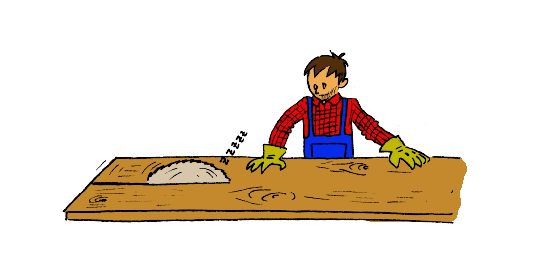
\includegraphics[width=5cm]{menuisier} \end{center}

Complète alors l'égalité $478,8 = 9 \cdot \ldots + \ldots$ . \label{NbEntDec_Approf81Qa}

 \item En utilisant la division écrite au \ref{NbEntDec_Approf81Qa}, recopie et complète les égalités suivantes :
 \begin{itemize}  
  \item $47,88 = 9 \cdot 5,3 + \ldots$ ;
  \item $4 788 = 9 \cdot 532 + \ldots$ ;
  \item $4 788 = 90 \cdot 53 + \ldots$ ;
  \item $4,788 = 9 \cdot \ldots + 0,018$.
  \end{itemize}
 \end{enumerate}
\end{exercice}


\begin{exercice}[Paquets empilés]
On a reçu au collège 7 rames de 500 feuilles pour la photocopieuse et 3 paquets de 24 pièces de « carton plume » :
\begin{enumerate}
 \item L'épaisseur d'une feuille de papier pour photocopieuse est de 0,11 mm et celle d'une pièce de « carton plume » est de 5 mm. Calcule un ordre de grandeur de la hauteur totale de tous ces paquets empilés ;
 \item Écris la hauteur totale des paquets en une seule expression puis calcule‑la.
 \end{enumerate}
\end{exercice}


\begin{exercice}[Densité de population]
On considère le tableau suivant :

\begin{center}
\begin{tabularx}{\linewidth}{|c|*{6}{>{\centering \arraybackslash}X|}}
\hline \rowcolor{U1} Continent & Nombre d'habitants & Superficie en km\up{2} \\
\hline \rowcolor{A3} Afrique & 965 millions & 30\,206\,704 \\
\hline \rowcolor{A3} Amérique & 911 millions & 42\,189\,120 \\
\hline \rowcolor{A3} Asie & 4,03 milliards & 43\,810\,582 \\
\hline \rowcolor{A3} Europe & 731 millions & 10\,180\,000 \\
\hline \rowcolor{A3} Océanie & 34 millions & 9\,008\,458 \\
\hline
\end{tabularx} \\
\end{center}

\begin{enumerate}
 \item Quel est le continent qui a le plus grand nombre d'habitants ? Et le plus petit nombre ?
 \item Quel est le continent qui a la plus grande superficie ? Et la plus petite ?
 \item Pour chaque continent, calcule la densité de population exprimée en habitants par km\up{2}. Tu donneras une valeur approchée à l'unité. 
 \item Ces résultats sont‑ils surprenants ? Explique.
 \item Calcule le nombre moyen d'habitants au km\up{2} dans le monde. Indique les continents qui sont en dessous de cette moyenne et ceux qui sont au dessus. 
 \end{enumerate}
\end{exercice}


\begin{exercice}[Football]
Le match de football entre le FC Barcelone et le Milan AC a eu lieu mardi soir 1\up{er} novembre à Barcelone. 
\begin{enumerate}
 \item Sachant qu’un match de football se joue en 2 mi-temps de 45 minutes séparées par une pause de 15 minutes, qu’il y a eu en tout 4 minutes d’arrêt de jeu en première mi-temps et 3 minutes en seconde mi-temps et que la rencontre a débuté à 20h45, trouver l’heure à laquelle le match s’est terminé. 
 \item Yvan, joueur de FC Barcelone est sorti du terrain au bout de 22 minutes de jeu en deuxième mi-temps, calculer l’heure à laquelle ce changement a eu lieu.
 \item Les supporters du Milan AC, qui avaient effectué le déplacement en autocar ont quitté le stade à 23h15 min. Sachant que leur voyage de retour a duré 16h40, calculer l’heure exacte et la date précise à laquelle ils sont arrivés à Milan. 
 \end{enumerate}
\end{exercice}
\end{colonne*exercice}

\connaissances
\begin{acquis}
\begin{itemize}
\item BlaBla1
\item BlaBla2
\item BlaBla3
\item BlaBla4
\item BlaBla5
\item BlaBla6
\end{itemize}
\end{acquis}

%%%%%%%%%%%%%%%%%%%%%%%%%%%%%%%%%%%%%%%%%%%%%%%%%%%%%%%%%%%%%%%%%%%%%%%%%%%

\QCMautoevaluation{Pour chaque question, plusieurs réponses sont % enlever l'adresse internet.
  proposées.  Déterminer celles qui sont correctes.} 

\begin{QCM}
  \begin{GroupeQCM} 
    \begin{exercice}
      Dix-huit millions huit cents s'écrit :
      \begin{ChoixQCM}{4}
      \item 18\,800\,000
      \item 18\,000\,800
      \item 18\,800
      \item 18\,008\,100
      \end{ChoixQCM}
\begin{corrige}
     \reponseQCM{a} % J'ai mis "a" partout
   \end{corrige}
    \end{exercice}

    \begin{exercice}
      45 centaines est égal à :
      \begin{ChoixQCM}{4}
      \item 5 unités
      \item 450 dizaines
      \item 4 dizaines
      \item 45\,100
      \end{ChoixQCM}
      \begin{corrige}
     \reponseQCM{a}
   \end{corrige}
    \end{exercice}

    
    \begin{exercice}
      Un centième est :
      \begin{ChoixQCM}{4}
      \item plus grand qu'un dixième
      \item égal à dix millièmes
      \item plus petit qu'un millième
      \item égal à dix  dixièmes
      \end{ChoixQCM}
      \begin{corrige}
     \reponseQCM{a}
   \end{corrige}
    \end{exercice}


    \begin{exercice}
      Une écriture décimale de 456 centièmes est :
      \begin{ChoixQCM}{4}
      \item 456,100
      \item 456\,100
      \item 4,56
      \item 4\,560 millièmes
      \end{ChoixQCM}
      \begin{corrige}
     \reponseQCM{a}
   \end{corrige}
    \end{exercice}


    \begin{exercice}
      Le nombre $5 + 0,4 + 0,007$ peut aussi s'écrire :
      \begin{ChoixQCM}{4}
      \item 547 millièmes
      \item 5,47
      \item 5,407
      \item 5\,047 millièmes
      \end{ChoixQCM}
      \begin{corrige}
     \reponseQCM{a}
   \end{corrige}
    \end{exercice}
    
     \begin{exercice}
      7 unités, 8 centièmes et 5 millièmes s'écrit :
      \begin{ChoixQCM}{4}
      \item 7,85
      \item 7,085
      \item 7,800\,500\,0
      \item 7,085\,0
      \end{ChoixQCM}
      \begin{corrige}
     \reponseQCM{a}
   \end{corrige}
    \end{exercice}

     \begin{exercice}
      Dans l'écriture décimale du nombre 45,631...
      \begin{ChoixQCM}{4}
      \item la valeur du chiffre 3 est dix fois moins grande que celle du chiffre 6
      \item 6 est le chiffre des centaines
      \item la valeur du chiffre 4 est deux fois plus grande que celle du chiffre 6
      \item 0,631 est la partie décimale
      \end{ChoixQCM}
      \begin{corrige}
     \reponseQCM{a}
   \end{corrige}
    \end{exercice}

     \begin{exercice}
      Un nombre compris entre 24,56 et 24,57 est par exemple...
      \begin{ChoixQCM}{4}
      \item 24\,568 millièmes
      \item 24,560\,7
      \item impossible, il n'y a pas de nombre compris entre 24,56 et 24,57
      \item $42 + 0,562$
      \end{ChoixQCM}
      \begin{corrige}
     \reponseQCM{a}
   \end{corrige}
    \end{exercice}
    
     \begin{exercice}
      L'arrondi de 123,254 au dixième est...
      \begin{ChoixQCM}{4}
      \item 120
      \item 123,2
      \item 123,26
      \item 123,3
      \end{ChoixQCM}
      \begin{corrige}
     \reponseQCM{a}
   \end{corrige}
    \end{exercice}

     \begin{exercice}
      873,023 est ...
      \begin{ChoixQCM}{4}
      \item 1\,000 fois plus grand que 873\,230
      \item 100 fois plus petit que 87\,302,3
      \item 10\,000 fois plus grand que 0,087\,302\,3
      \item 10 fois plus petit que 87,302\,3
      \end{ChoixQCM}
      \begin{corrige}
     \reponseQCM{a}
   \end{corrige}
    \end{exercice}
    
     \begin{exercice}
      $57,41 - 27,83 =$ ...
      \begin{ChoixQCM}{4}
      \item 30.42
      \item 30.58
      \item 29.58
      \item 19.58
      \end{ChoixQCM}
      \begin{corrige}
     \reponseQCM{a}
   \end{corrige}
    \end{exercice}
 \end{GroupeQCM}  
 \end{QCM}  
    
    
    
    
    
 \begin{QCM}
\begin{GroupeQCM}
     \begin{exercice}
      $872,967 =$ ...
      \begin{ChoixQCM}{4}
      \item $87\,296,7 \div 100$
      \item $862,967 \cdot10$
      \item $87,296\,7 \cdot 10$
      \item $8,729\,67 \cdot 100$
      \end{ChoixQCM}
      \begin{corrige}
     \reponseQCM{a}
   \end{corrige}
    \end{exercice}
    
     \begin{exercice}
      $78,23 \cdot 21,796 =$ ...
      \begin{ChoixQCM}{4}
      \item 170\,510,108
      \item 3\,705,101\,08
      \item 1\,705,101\,08
      \item 1\,800
      \end{ChoixQCM}
      \begin{corrige}
     \reponseQCM{a}
   \end{corrige}
    \end{exercice}
    
     \begin{exercice}
      $34,1 + 123,79$ se pose ...
      \begin{ChoixQCM}{4}
      \item 
      
      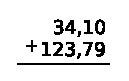
\includegraphics[width=1.5cm]{frac1}
      \item 
      
      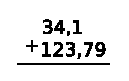
\includegraphics[width=1.5cm]{frac2}
      \item 
      
      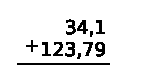
\includegraphics[width=1.7cm]{frac3}
      \item 
      
      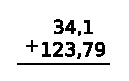
\includegraphics[width=1.5cm]{frac4}
      \end{ChoixQCM}
      \begin{corrige}
     \reponseQCM{a}
   \end{corrige}
    \end{exercice}

    
     \begin{exercice}
      Une ficelle mesure 7,2 m. On la partage en 16.
      \begin{ChoixQCM}{4}
      \item Chaque bout mesure 1,152 m
      \item C'est impossible, $16 > 7,2$
      \item Chaque bout mesure environ 2,2 m
      \item Chaque bout mesure 45 cm
      \end{ChoixQCM}
      \begin{corrige}
     \reponseQCM{a}
   \end{corrige}
    \end{exercice}
    
    \begin{exercice}
      0,75 peut être la réponse du (ou des) problème(s) suivant(s) :
      \begin{ChoixQCM}{4}
      \item Avec 126 litres d'eau, on a rempli 168 bouteilles. Quelle est la contenance d'une bouteille ?
      \item Une baignoire peut contenir 223,24 L. On la remplit avec  222,49 L d'eau. Combien d'eau peut‑on encore verser ?
      \item Ahmed achète un bonbon à 0,27 CHF et un chewing‑gum à 0,58 CHF. Combien paye‑t‑il ?
      \item 125 CD de 6 mm d'épaisseur sont empilés. Quelle est la hauteur en mètre de la pile ?
      \end{ChoixQCM}
      \begin{corrige}
     \reponseQCM{a}
   \end{corrige}
    \end{exercice}
    
    \begin{exercice}
      Henri court pendant 1 h 52 min. Il s'arrête à 10 h 07. Il est parti à...
      \begin{ChoixQCM}{4}
      \item 8 h 55
      \item 11 h 59
      \item 8 h 15
      \item 9 h 45
      \end{ChoixQCM}
      \begin{corrige}
     \reponseQCM{a}
   \end{corrige}
    \end{exercice}

\end{GroupeQCM}
\end{QCM}

  

\TravauxPratiques % pour nous "travailler en groupe"

\begin{TP}[]
Voici un extrait de « La Disme », écrit par Simon Stevin en 1585 : \\[0.3em]

« Les 27 \circled{0} 8 \circled{1} 4 \circled{2} 7 \circled{3} donnés, font ensemble 27 $\dfrac{8}{10}$, $\dfrac{4}{100}$, $\dfrac{7}{1\,000}$, ensemble 27 $\dfrac{847}{1\,000}$, et par même raison les 37 \circled{0} 6 \circled{1} 7 \circled{2} 5 \circled{3} valent 37 $\dfrac{675}{1\,000}$. Le nombre de multitude des signes, excepté \circled{0}, n'excède jamais le 9. Par exemple nous n'écrivons pas 7 \circled{1} 12 \circled{2}, mais en leur lieu 8 \circled{1} 2 \circled{2}. »

\partie{Simon Stevin}

Par groupe, en vous documentant, répondez aux questions suivantes.
\begin{enumerate}
 \item Où Simon Stevin a-t-il vécu ?
 \item Quels sont les domaines dans lesquels Simon Stevin a travaillé ? Faites la synthèse des réponses de chaque groupe.

\partie{La Disme} % Pourquoi cette ligne est si rentrée ?

\item Cherchez comment on écrit de nos jours le nombre 38 \circled{0} 6 \circled{1} 5 \circled{2} 7 \circled{3}­.

Comparez avec les réponses des autres groupes.

\item Écrivez, à la manière décrite par Simon Stevin, les nombres $124 + \dfrac{7}{10} + \dfrac{5}{100}$ et 34,802.

Comparez avec les réponses des autres groupes.

 \item Choisissez trois nombres décimaux différents et écrivez-les à la manière décrite par Simon Stevin.
 \item échangez ensuite avec un autre groupe ces nombres écrits à la manière de Simon Stevin. Cherchez alors comment on écrit de nos jours les nombres que vous avez reçus.
 \item Faites une recherche pour trouver les différentes notations utilisées depuis 1585 pour l'écriture des nombres décimaux.
 \end{enumerate}
\end{TP}

%%%%%%%%%%%%%%%%%%%%%%%%%%%%%%%%%%%%%%%%%%%%%%%%%%%%%%%%%%%%%%%%%%%%%%%%%%%

\begin{TP}[Compétitions dans la classe]
Préparatifs : fabriquez une étiquette de carton pour chaque élève de la classe, comportant son nom et son prénom. Mélangez ces étiquettes.

Voici un exemple de liste de calculs à effectuer :
\begin{enumerate}
 \item $853,12 + 19,7$ ;
 \item $538,21 - 42,16$ ;
 \item $65,24 \cdot 7,38$ ;
 \item $68,37 : 3$.
 \end{enumerate}

\partie{Entraînement en individuel (appelé 1 contre 10)}
Pour chaque manche, un élève $A$ est tiré au sort à l'aide des étiquettes et passe au tableau où un seul calcul écrit est à effectuer. \\[0.5em]
L'élève $A$ l'effectue en public pendant que tous les autres cherchent chacun sur une feuille. \\[0.5em]
Dès qu'un élève a trouvé la réponse et a écrit le calcul, il lève la main. Le professeur surveille le tableau et circule dans la classe pour vérifier le travail de chaque élève. \\[0.5em]
Il compte à haute voix de 1 à 10 en ajoutant 1 chaque fois qu'un travail est considéré comme correct. \\[0.5em]
Arrivé à 10, si l'élève $A$ n'a pas trouvé, la classe a gagné la manche. Par contre, si l'élève $A$ trouve avant la fin du décompte à 10, c'est lui qui a gagné.

\partie{Par équipes (appelé 2 contre 5)}
On constitue des binômes équilibrés d'élèves.\\[0.5em]
Lors du tirage au sort, l'élève $A$ désigné passe au tableau accompagné de son coéquipier mais seul l'élève $A$ peut écrire. \\[0.5em]
On démarre la compétition comme dans le « 1 contre 10 » mais le professeur ne compte que jusqu'à 5. 
\end{TP}

\pagebreak

\Recreation
\begin{enigme}[La constante de Champernowne]

Ce nombre, inventé par le mathématicien anglais David Gawen Champernowne en 1933, commence par

0,123456789101112131415 \ldots . \\[-1em]
\begin{enumerate}
 \item Quelle est la particularité de cette constante ? Donne les dix décimales suivantes.
 \item Quelle est l'arrondi, au cent-milliardième près, de cette constante ?
 \end{enumerate}
 \end{enigme}
        
\vspace*{2em}
        
\begin{enigme}[Défis]
Combien de fois faudrait-il utiliser le chiffre 1 si l'on voulait écrire tous les nombres entiers de 1 à 999 ? Et le chiffre 9 ?

Donne le nombre de mots utilisés pour écrire tous les entiers plus petits que 100.
 \end{enigme} 
 
 \vspace*{2em}

\begin{enigme}[Calculatrices infernales 1 (d'après Apmep)]
Sur la calculatrice d'Aïsha, la touche pour afficher la virgule ne fonctionne plus et la touche « $=$ » ne peut fonctionner qu'une seule fois par ligne de calcul.

Comment peut‑elle trouver le résultat de $(17,32 \cdot 45,3) + 15,437$ ?
 \end{enigme} 
 
 \vspace*{2em}

\begin{enigme}[Calculatrices infernales 2 (d'après Apmep)]
Bruce vient de faire tomber sa calculatrice. Elle ne comporte plus que les chiffres, la virgule et les quatre opérations, mais quand on appuie sur « $+$ » elle ajoute 1, quand on appuie sur « $-$ » elle retranche 1, quand on appuie sur la touche « $\times$ » elle multiplie par 10 et quand on appuie sur la touche « $\div$ » elle divise par 10. \\[-1em]
\begin{enumerate}
 \item Romain emprunte la calculatrice de Bruce. Il tape 27,2 puis appuie ensuite sur les touches « $\times$ », « $\times$ », « $+$ », « $+$ », « $-$ », « $\div$ », « $\div$ », « $\div$ », « $+$ », « $\times$ ». Quel résultat Romain trouve-t-il ?
 \item Comment peut‑il passer en sept opérations :    
 \begin{colitemize}{3}
  \item de 3,14 à 300 ?
  \item de 3,14 à 297 ?
  \item de 297 à 0,2 ?
  \end{colitemize}
 \item Tu viens de passer de 3,14 à 0,2 en quatorze opérations. Trouve un chemin qui permette de faire cela avec le minimum d'opérations. Compare avec tes camarades ; \\[0.5em]
Trouve un chemin qui permette de passer de 5 à 4,99 en un minimum d'opérations puis compare avec tes camarades.
 \end{enumerate}
\end{enigme} 





\themaG
\chapter{Points, segments, droites, cercles et angles}

\activites

\begin{activite}[Segments, droites et demi-droites]

 \begin{partie}[À la découverte d'un nouveau code]
  \begin{enumerate}
   \item Lire la consigne de la case \circled{1} et observer la figure correspondant à cette consigne.
Faire de même pour la case \circled{2}.

Quand le code est compris, tracer la figure de la case \circled{3} et écrire la consigne de la case \circled{4}.


  \vspace{1em}
  
  
  
  \begin{tabular}{|c|c|c|c|c|}
  \cline{1-2}\cline{4-5}
    \circled{1} 		& \circled{2} 		& 	& \circled{3} 		& \circled{4}	\\ 
     Tracer $(AB)$ 	&  Tracer $[AC)$ 	& 	& Tracer $(AB)$	& 	 		\\ 
     Tracer $[AC]$ 	& Tracer $[BC]$ 	& 	& Tracer$[BC]$		& 			\\
     				&				&	& Tracer$[AC)$		&			\\ \cline{1-2}\cline{4-5}
   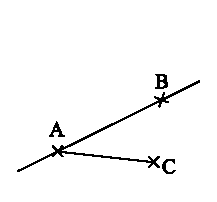
\includegraphics[width=.2\linewidth]{tracerAB-AC} & 
   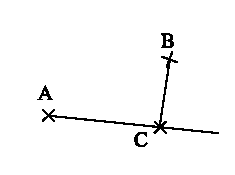
\includegraphics[width=.2\linewidth]{tracerAC-BC} & & 
   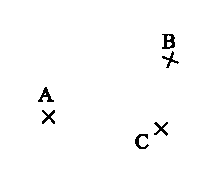
\includegraphics[width=.2\linewidth]{tracerAB-BC-AC}& 
   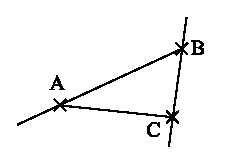
\includegraphics[width=.2\linewidth]{tracer} 					\\ \cline{1-2}\cline{4-5}
  \end{tabular}\\[1em]

  
   \item Lire la consigne de la case \circled{5} et observer la figure correspondant à cette consigne. Tracer ensuite la figure de la case \circled{6} et écrire la consigne de la case \circled{7}.
   
   \vspace{1em}
  
    \begin{tabular}{|l|l|l|}
   \hline
    \hfill \circled{5} \hfill			&	\hfill \circled{6} \hfill				&	\hfill \circled{7} \hfill 	\\
    - Tracer la droite passant par 	&	- Tracer le segment 				&					\\
    $E$ et $F$ ;					&	d'extrémités $R$ et $S$ ;			&					\\
    - Tracer le segment 			&	- Tracer la droite passant par 		&					\\
    d'extrémités $E$ et $G$ ;		&	$R$ et $T$ ;					&					\\
    - Tracer la demi-droite 			&	- Tracer la demi-droite 			&					\\
    d'origine $G$ et passant par $F$.	&	d'origine $S$ et passant par $T$.	&					\\ \hline
    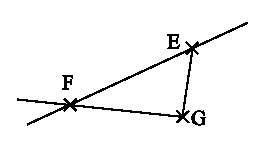
\includegraphics[width=.24\linewidth]{tracerEFG} 			&  
    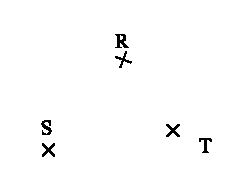
\includegraphics[width=.24\linewidth]{tracerRST}			&
    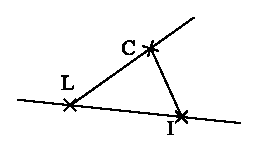
\includegraphics[width=.24\linewidth]{tracerLCI}			\\ \hline
    \end{tabular}\\[1em]

    
  \newpage
  
   \item Compléter le tableau suivant :
   
   \vspace{1em}
   
   \renewcommand*\tabularxcolumn[1]{>{\centering\arraybackslash}m{#1}}
   \begin{ttableau}{\linewidth}{3}
    \hline
    \multicolumn{1}{|c|}{\textbf{Phrase}}	&	\multicolumn{1}{c}{\textbf{Phrase codée}}	&	\multicolumn{1}{|c|}{\textbf{Dessin}}			 	\\  \hline
    								&	Tracer $[UV]$							&	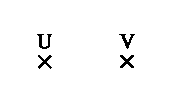
\includegraphics[width=2.6cm]{phraseUV}		\\  \hline
    								&										&	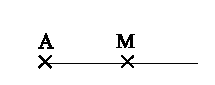
\includegraphics[width=3.2cm]{phraseAM}		\\  \hline
   Tracer la droite passant par $S$ et $T$	&										&	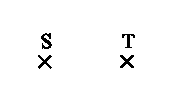
\includegraphics[width=2.6cm]{phraseST}		\\  \hline
   								&										&	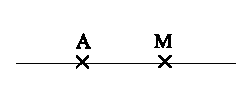
\includegraphics[width=4.0cm]{phraseAM_2}	\\  \hline
   Tracer le segment d'extrémités $M$ et $N$	&									&	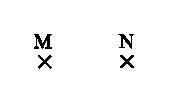
\includegraphics[width=2.6cm]{phraseMN} 	\\  \hline
   								&	Tracer $[KJ)$							&	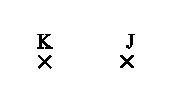
\includegraphics[width=2.6cm]{phraseKJ}		\\  \hline
								&										&	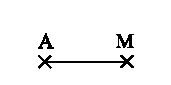
\includegraphics[width=2.6cm]{phraseAM_3}	\\  \hline
   Tracer la demi-droite d'origine $O$ et 	&										&	
\includegraphics[width=2.6cm]{phraseOU}		\\
   passant par $U$					&										&										\\  \hline
   								&	Tracer $(BC)$							&	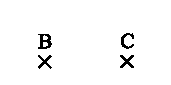
\includegraphics[width=2.6cm]{phraseBC}		\\  \hline
  \end{ttableau}
  
   \end{enumerate} 

  \end{partie}

\end{activite}

\newpage

%%%%%%%%%%%%%%%%%%%%%%%%%%%%%%%%%%%%%%%%%%%%%

\begin{activite}[Repérer des droites perpendiculaires]

 \begin{minipage}[c]{0.50\linewidth}
  \begin{partie}[Éric a oublié son équerre !]
 
  « Pas de souci, lui dit son professeur, prends une feuille blanche non quadrillée. Tu devrais pouvoir obtenir un angle droit en pliant deux fois cette feuille. »
  
  Réalise une telle équerre.
  
  Qu'obtiens‑tu si tu déplies ta feuille ? 
    \end{partie}
  
  \begin{partie}[Éric utilise sa nouvelle équerre \ldots]
  
  Éric doit replacer l'équerre dans la position qui a permis de construire les droites $d_4$ et $d_7$. \\[0.5em]
  Place l'équerre dans cette position. \\[0.5em]
  Trouve alors un autre couple de droites \textbf{perpendiculaires} sur cette figure en t'aidant de ton équerre.
    \end{partie} \end{minipage} \hfill %
   \begin{minipage}[c]{0.44\linewidth}
   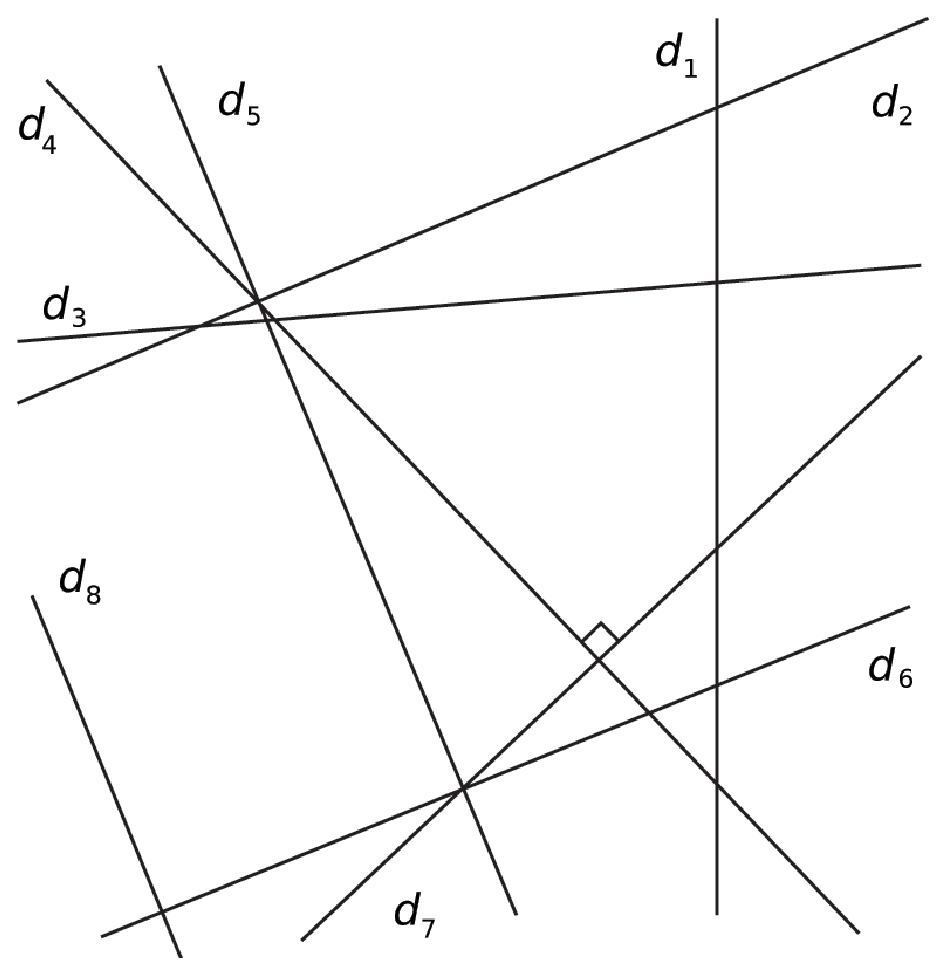
\includegraphics[width=6.1cm]{plusieurs_droites}
   \end{minipage} \\

 \begin{partie}[Utilisation de l'équerre d'Éric]
 
Trace deux droites sécantes $d$ et $d'$. À l'aide de l'équerre que tu as fabriquée, construis une droite perpendiculaire à $d$ et une autre perpendiculaire à $d'$. Tu n'oublieras pas d'ajouter les codages nécessaires.

  \end{partie} 
  
\end{activite}

%%%%%%%%%%%%%%%%%%%%%%%%%%%%%%%%%%%%%%%%%%%%%

\begin{activite}[Droites parallèles]

 \begin{partie}[Deux droites perpendiculaires]
 
  \begin{enumerate}
   \item Place deux points $A$ et $B$.
   \item Trace une droite $d$ ne passant ni par $A$, ni par $B$ et qui coupe $(AB)$.
   \item Trace $d_1$ la perpendiculaire à d passant par $A$, puis la droite $d_2$ perpendiculaire à $d_1$ passant par $B$. Que remarques‑tu ?
   \item Trace $d_3$ la perpendiculaire à $d$ passant par $B$ et $d_4$ la perpendiculaire à $d_3$ passant par $A$. Que peux‑tu dire de $d_2$ et $d_4$ ? Quelles autres remarques du même type peux‑tu faire ? 
   \end{enumerate}
   
  \end{partie} 

 \begin{partie}[Construction à la règle et à l'équerre]
 
 \begin{minipage}[c]{0.66\linewidth}
 La première vignette d'une bande dessinée est représentée ci‑contre. On y a placé une droite $d$ et un point $A$ n'appartenant pas à $d$.
 Complète cette bande dessinée pour expliquer comment, à l'aide de la règle et de l'équerre, tu traces la \textbf{parallèle} à $d$ passant par $A$.
  \end{minipage} \hfill %
 \begin{minipage}[c]{0.3\linewidth}
 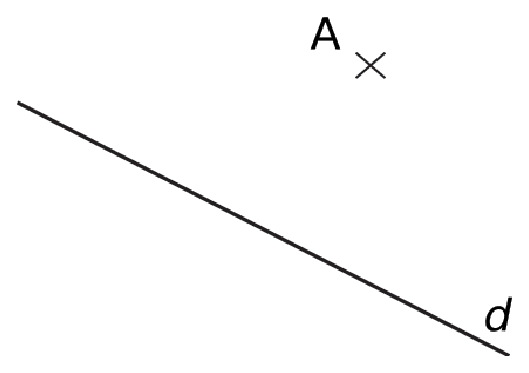
\includegraphics[width=4.2cm]{droiteAd}
  \end{minipage} \\
 
  \end{partie} 

\end{activite}

%%%%%%%%%%%%%%%%%%%%%%%%%%%%%%%%%%%%%%%%%%%%%

\begin{activite}[Tout savoir sur la médiatrice !]

 \begin{partie}[Axes de symétrie d'un segment]
 
 \begin{enumerate}
  \item Sur une feuille blanche, trace un segment $[AB]$.
  \item Plie cette feuille de manière à ce que le point $A$ touche le point $B$, cela fait apparaître un axe de symétrie de ce segment. Le symétrique de $A$ par rapport à cet axe est $B$. Comment s'appelle cet axe ? Repasse‑le en couleur.
  \item Quelles sont ses caractéristiques ?
  \end{enumerate}
  
  \end{partie}
  
 \begin{partie}[Propriété d'un point appartenant à la médiatrice d'un segment]
 
 \begin{enumerate}
  \item Place un point $M$ sur cette médiatrice. Que dire des longueurs $AM$ et $BM$ ?
  \item Que dire alors d'un point qui appartient à la médiatrice d'un segment ?
  \end{enumerate}
  
  \end{partie}
  
 \begin{partie}[Ensemble de points]
 
 \begin{minipage}[c]{0.76\linewidth}
 \begin {enumerate}
  \item Construis un segment $[CD]$ de longueur 5 cm. 
  \item Place $A$, \textbf{équidistant} de $C$ et de $D$. Place trois autres points équidistants de $C$ et de $D$. 
  \item Où semblent se trouver tous les points équidistants de $C$ et $D$ ?
  \item Que dire d'un point équidistant des extrémités d'un segment ?
  \item Déduis‑en une façon de construire la médiatrice d'un segment sans l'équerre. 
  \end{enumerate} 
  \end{minipage} \hfill %
 \begin{minipage}[c]{0.2\linewidth}
 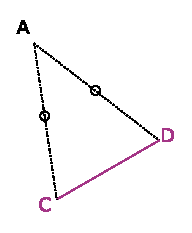
\includegraphics[width=2.8cm]{triangleACD}
  \end{minipage} \\
  
 \end{partie}

\end{activite}

%%%%%%%%%%%%%%%%%%%%%%%%%%%%%%%%%%%%%%%%%%%%%

\begin{activite}[Bissectrice, qui es-tu ?]

 \begin{partie}[Définition] \label{EntDroitSeg_DefBissectrice}

 \begin{minipage}[c]{0.68\linewidth}
 \begin {enumerate}
  \item Sur une feuille blanche, trace un angle $\widehat{ABC}$.
  \item Plie cette feuille de façon à faire apparaître l'axe de symétrie de l'angle. Repasse‑le en couleur. Place un point D sur cet axe (comme sur le croquis ci contre). \label{EntDroitSeg_plier}
  \item Cet axe fait apparaître deux nouveaux angles. Nomme‑les.
  \item Que peut‑on dire de la mesure de ces deux angles ? Justifie. Comment nomme‑t‑on cette droite ?
  \end{enumerate} 
  \end{minipage} \hfill %
 \begin{minipage}[c]{0.26\linewidth}
 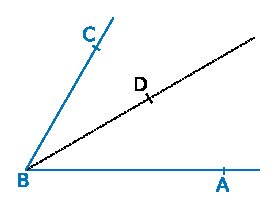
\includegraphics[width=3.8cm]{bissectrice}
  \end{minipage} \\
  
 \end{partie}
 
 \begin{partie}[Construction au compas]
 
 \begin{enumerate}
 \item Construis le point $A'$ symétrique du point $A$ par rapport à la bissectrice de l'angle $\widehat{ABC}$ Tu obtiens ce point en reportant le point A sur la droite $[BC)$ en pliant la feuille comme au point \ref{EntDroitSeg_plier} de la partie \ref{EntDroitSeg_DefBissectrice}. Que dire des longueurs $BA$ et $BA'$ ?
 \item Que représente la bissectrice de l'angle $\widehat{ABC}$ pour le segment $[AA']$ ?
 \item Déduis‑en une façon de construire la bissectrice d'un angle sans rapporteur.
  \end{enumerate}              
  \end{partie}
 
\end{activite}

%%%%%%%%%%%%%%%%%%%%%%%%%%%%%%%%%%%%%%%%%%%%%

\begin{activite}[De qui est-ce la trace ?]

 \begin{partie}
 Sur ton cahier, place un point $O$. Recherche tous les points situés à 3 cm du point $O$. 
  \end{partie}

 \begin{partie}
 \begin{minipage}[c]{0.78\linewidth}
 Un système d'arrosage automatique est formé d'un jet qui arrose dans toutes les directions jusqu'à 4 m.
  \begin {enumerate}
  \item Représente sur ton cahier la zone arrosée par le jet en appelant $J$ l'emplacement du jet. (1 cm représentera 1 m.)
  \item Comment peux‑tu définir les points de la zone arrosée ? 
  \end{enumerate} 
  \end{minipage} \hfill %
 \begin{minipage}[c]{0.16\linewidth}
 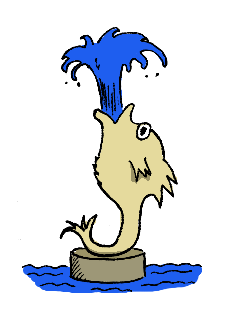
\includegraphics[width=2cm]{arrosage}
  \end{minipage} \\
    
  \end{partie}

\end{activite}

%%%%%%%%%%%%%%%%%%%%%%%%%%%%%%%%%%%%%%%%%%%%%

\begin{activite}[Des constructions]

 \begin{partie}[Du programme à la figure]
 Réalise la suite d'instructions suivantes :
 \begin{itemize}
  \item Trace un cercle $(\mathcal{C})$ de centre $O$ et de rayon 5 cm.
  \item Place, sur le cercle, deux points $A$ et $B$ \textbf{diamétralement opposés}.
  \item Construis le cercle $(\mathcal{C}_1)$ de diamètre $[OA]$ et le cercle $(\mathcal{C}_2)$ de diamètre $[OB]$.
  \item Trace le cercle $(\mathcal{C}_3)$ de centre $A$ passant par $O$.
  \item Nomme $E$ et $F$ les \textbf{points d'intersection} des cercles $(\mathcal{C})$ et $(\mathcal{C}_3)$.
  \item Trace le cercle $(\mathcal{C}_4)$ de centre $B$ et de rayon $OB$.
  \item Les cercles $(\mathcal{C})$ et $(\mathcal{C}_4)$ se coupent en $G$ et $H$.
  \end{itemize}
  
  \end{partie}
  
  \vspace{2em}
  
 \begin{partie}[De la figure au programme]
 \begin{minipage}[c]{0.48\linewidth} 
Construis la figure ci‑contre donnée 

par son croquis.

Écris le programme de construction.
 \end{minipage} \hfill %
 \begin{minipage}[c]{0.46\linewidth}
 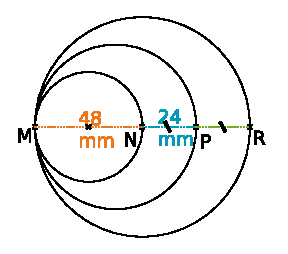
\includegraphics[width=4.2cm]{figure-programme}
  \end{minipage} \\
  
  \end{partie}

\end{activite}

%%%%%%%%%%%%%%%%%%%%%%%%%%%%%%%%%%%%%%%%%%%%%


\cours
\section{Les angles}

%%%%%%%%%%%%%%%%%%%%%%%%%%%%%

% remarque : pour qu'un mot se retrouve dans le lexique : \MotDefinition{asymptote horizontale}{} 

\begin{definition}
Un \MotDefinition{angle}{} est une portion de plan délimitée par deux demi-droites ayant la même origine.
 \end{definition}

\subsection{Reconnaître les différents types d'angles}

On classe les angles par catégories selon leur mesure.

 \renewcommand*\tabularxcolumn[1]{>{\centering\arraybackslash}m{#1}}
 \begin{ttableau}{\linewidth}{6}
\hline \textbf{Angle} 	&	Nul	&	Aigu		&	Droit		&	Obtus	&	Plat	\\ \hline
 \textbf{Figure} 	&	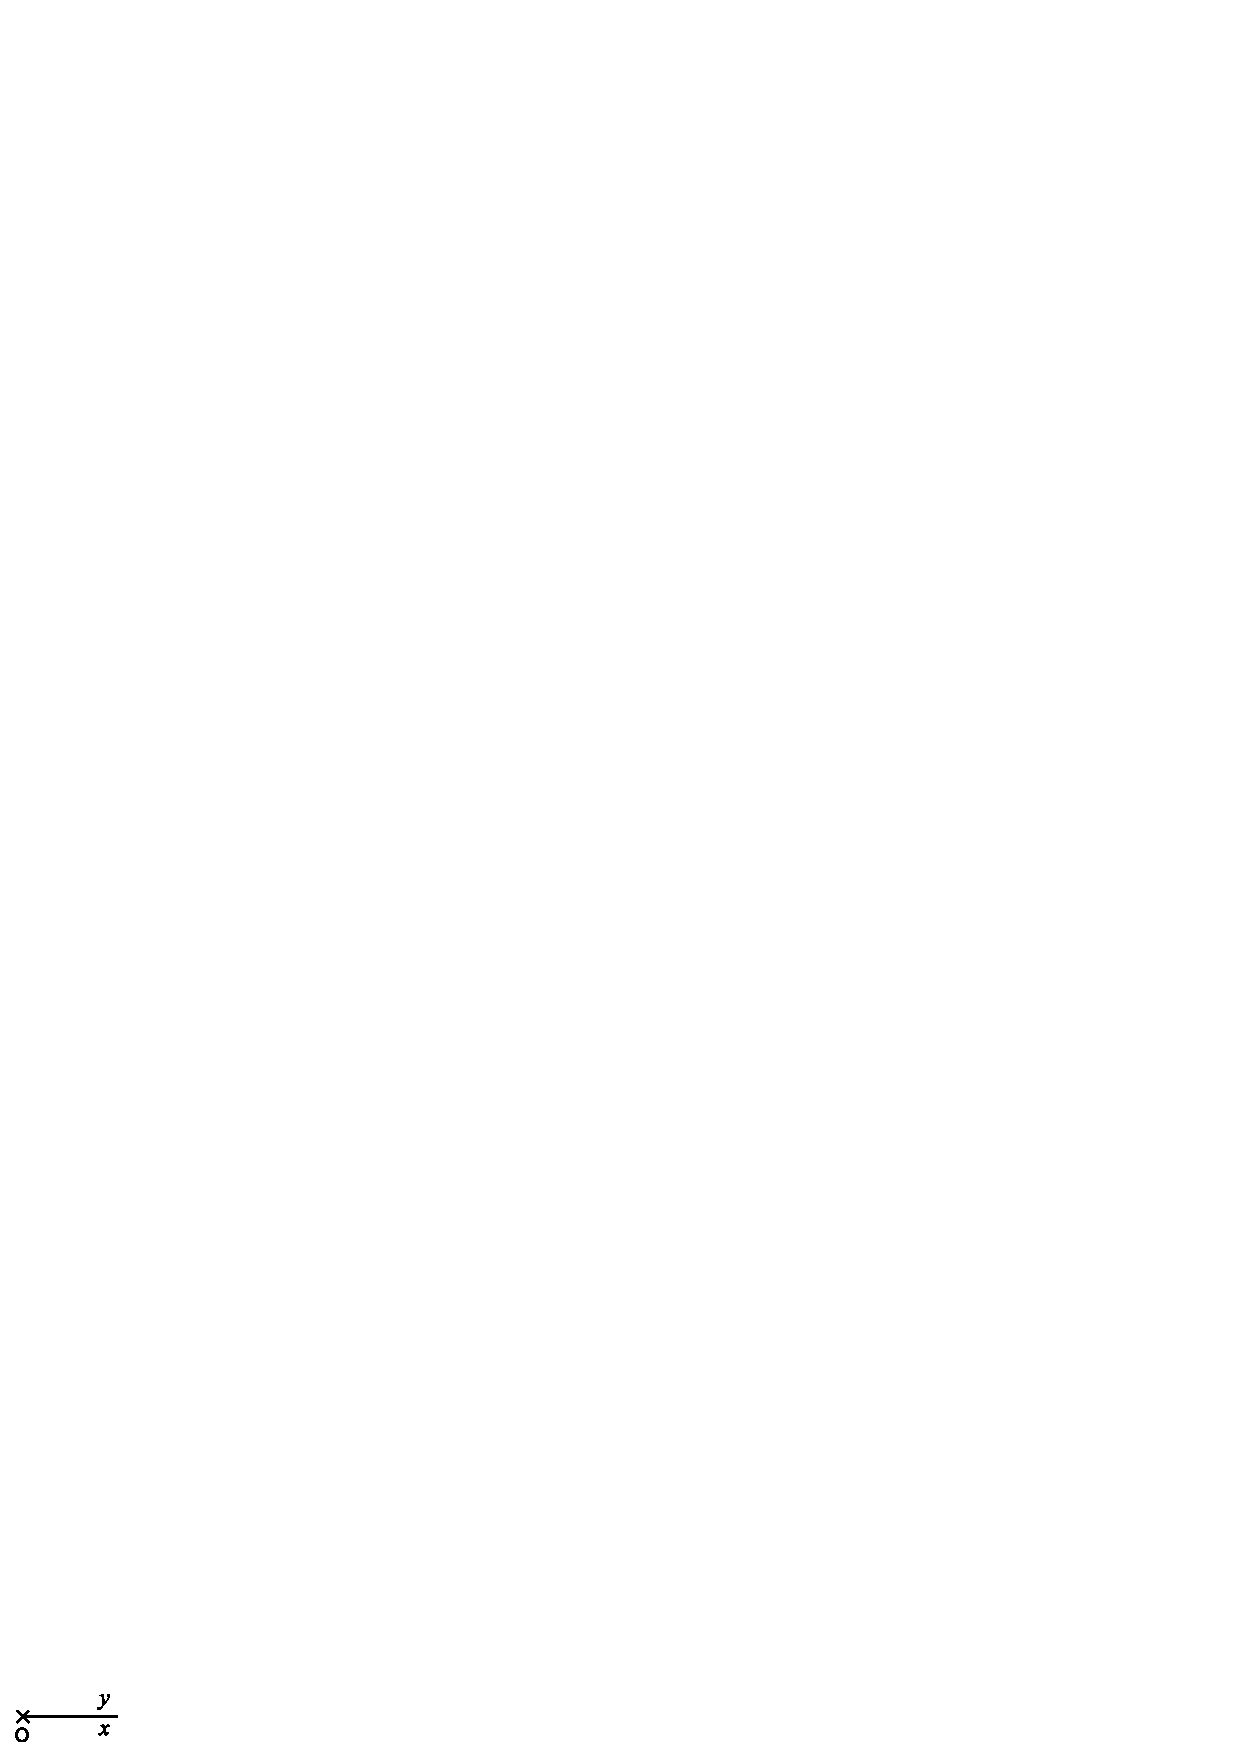
\includegraphics[width=1.7cm]{angle_nul}	&	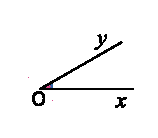
\includegraphics[width=1.7cm]{angle_aigu}	&	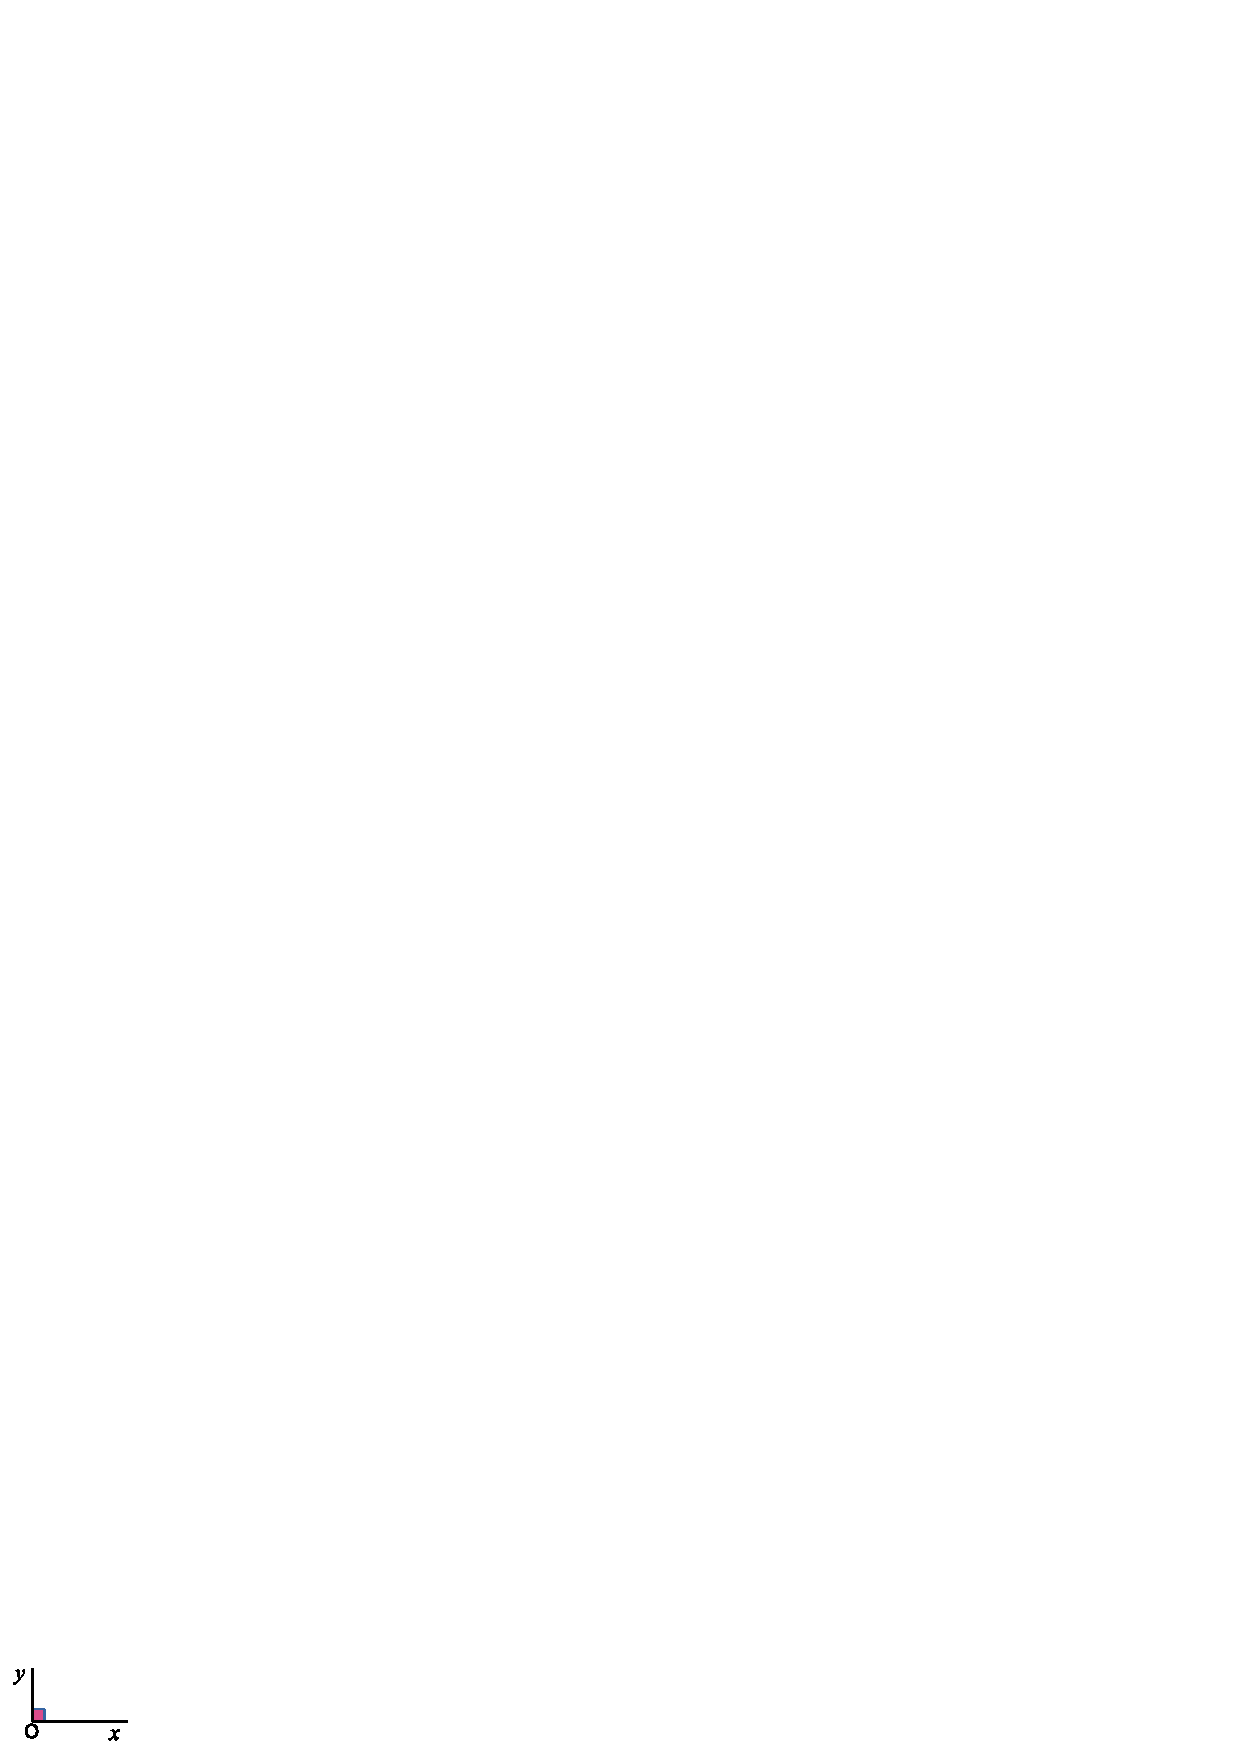
\includegraphics[width=1.7cm]{angle_droit}	&	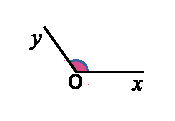
\includegraphics[width=1.7cm]{angle_obtus}	&	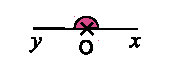
\includegraphics[width=1.7cm]{angle_plat}	\\ \hline
 \textbf{Mesure} 	&	$0^\circ$	&	entre $0^\circ$ et $90^\circ$	&	$90^\circ$		&	entre $90^\circ$ et $180^\circ$	&	 $180^\circ$	\\ \hline
 \multirow{3}{*}{\textbf{Position des côtés}} 	&		&	&	&	&	dans le 	\\ 
 	&	confondus		&	&	perpendiculaires	&	&	 prolongement	\\
	&	&	&	&	&	 l'un de l'autre	\\ \hline
 \end{ttableau}

%%%%%%%%%%%%%%%%%%%%%%%%%%%%%

\begin{methode*1}[Nommer un angle]

\begin{exemple*1}
Nomme l'angle marqué en violet sur la figure ci‑dessous.  \\[0.75em]

\begin{minipage}[c]{0.70\textwidth}
Le sommet de l'angle est le point $C$ : c'est la lettre centrale. \\[0.5em]
Les côtés de l'angle sont les demi‑droites $[CH)$ (ou $[Cx)$) et $[CS)$ (ou $[CA)$ (ou $[Cy)$). \\[0.5em]
Cet angle peut se nommer : $\widehat{{\textcolor{A1}{H}}C{\textcolor{C1}{S}}}$; $\widehat{{\textcolor{C1}{S}}C{\textcolor{A1}{H}}}$ ; $\widehat{{\textcolor{A1}{H}}C{\textcolor{C1}{A}}}$ ; $\widehat{{\textcolor{C1}{A}}C{\textcolor{A1}{H}}}$ ; $\widehat{{\textcolor{C1}{y}}C{\textcolor{A1}{x}}}$.
 \end{minipage} \hfill%
 \begin{minipage}[c]{0.26\textwidth}
 \includegraphics[width=3.8cm]{nommer_angle}
 \end{minipage} \\
 
\end{exemple*1}

\exercice 
Nomme les angles marqués sur la figure ci‑dessous. 
\begin{center} \includegraphics[width=4.5cm]{nommer_angles} \end{center}
%\correction
 
\end{methode*1}

%%%%%%%%%%%%%%%%%%%%%%%%%%%%%

\begin{methode*1}[Utiliser le rapporteur]

\begin{exemple*1}
Mesure l'angle $\widehat{CAB}$. \\[0.75em]

\begin{minipage}[c]{0.49\textwidth}
\centering
\includegraphics[width=4.8cm]{rapporteur1}
\end{minipage}\hfill%
 \begin{minipage}[c]{0.49\textwidth}%
 \centering
 \includegraphics[width=6.6cm]{rapporteur2}
  \end{minipage} \\
 \begin{minipage}[c]{0.43\textwidth}
On place le centre du rapporteur sur le sommet de l'angle.
\end{minipage} \hfill%
 \begin{minipage}[c]{0.53\textwidth}
 On place un zéro du rapporteur sur le côté $[AC)$. Si besoin, on prolonge la demi‑droite $[AC)$. La mesure de l'angle est donnée par l'autre côté de l'angle sur \underline{la même échelle} de graduation.
 \end{minipage} \\
  \end{exemple*1}
 
 \begin{exemple*1}
Construis un angle $\widehat{BUT}$ de $108^\circ$.  \\[0.75em]

\begin{minipage}[c]{0.49\textwidth}
\centering
\includegraphics[width=4.8cm]{rapporteur3}
\end{minipage}\hfill%
 \begin{minipage}[c]{0.49\textwidth}%
 \centering
 \includegraphics[width=6.6cm]{rapporteur4}
  \end{minipage} \\
 \begin{minipage}[c]{0.43\textwidth}
On trace $[UB)$, premier côté de l'angle. On place le centre du rapporteur sur le point $U$.
\end{minipage} \hfill%
 \begin{minipage}[c]{0.53\textwidth}
 On place un zéro du rapporteur sur le côté $[UB)$. On marque, d'un petit trait-repère, $108^\circ$ avec la bonne graduation.
On trace la demi‑droite d'origine $U$ passant par le repère. On place un point $T$ sur cette demi‑droite.
  \end{minipage} \\
  \end{exemple*1}
 
\exercice
 \begin{enumerate}
 \begin{minipage}[c]{0.36\textwidth}
  \item Mesure l'angle $\widehat{xOy}$ ci‑contre ;
  \item Construis un angle $\widehat{SAT}$ de $85^\circ$. 
  \end{minipage} \hfill%
 \begin{minipage}[c]{0.56\textwidth}
  \includegraphics[width=6cm]{angleyOx} 
  \end{minipage} \\
  \end{enumerate}
%\correction
 
\end{methode*1}

%%%%%%%%%%%%%%%%%%%%%%%%%%%%%

\section{Constructions graphiques : parallèles et perpendiculaires}

\begin{methode*1}[Construire la perpendiculaire à une droite passant par un point]

\begin{exemple*1}
Trace une droite $d$ et place un point $M$ n'appartenant pas à la droite $d$.

Trace la droite $d'$ perpendiculaire à la droite $d$ passant par le point $M$. \\[0.75em]

\begin{tabularx}{\textwidth}{X|X|X|X}
 \includegraphics[width=2.4cm]{droiteMxd} &  \includegraphics[width=2.4cm]{equerre} & \includegraphics[width=2.4cm]{regle} &  \includegraphics[width=2.4cm]{angledMd}\\ 
 On trace une droite $d$ et on place un point $M$. & On place l'un des côtés de l'angle droit de l'équerre sur la droite $d$ et l'autre côté sur $M$.
 & On prolonge la droite à la règle. & On nomme la droite $d'$ et on code l'angle droit par un carré.\\

\end{tabularx} \\
 
 \end{exemple*1}


\exercice

En utilisant cette méthode, tracer un rectangle ABCD de longueur 3 cm et de longueur 5 cm.

%\correction

 
\end{methode*1}

\newpage

%%%%%%%%%%%%%%%%%%%%%%%%%%%%%

\begin{methode*1}[Construire la parallèle à une droite passant par un point]

\begin{exemple*1}
Trace une droite $d$ et place un point $M$ n'appartenant pas à la droite $d$.

Trace la droite $d'$ parallèle à la droite $d$ passant par le point $M$. \\[0.75em]

\begin{tabularx}{\textwidth}{X|X|X|X}
 \includegraphics[width=2.4cm]{droiteMd} &  \includegraphics[width=2.4cm]{equerreMd} & \includegraphics[width=2.4cm]{equerre_regle} &  \includegraphics[width=2.4cm]{2droites}\\ 
On trace une droite $d$ et on place un point $M$. & On place l'un des côtés de l'angle droit de l'équerre sur la droite $d$. & On fait coulisser l'équerre le long de la règle, jusqu'au point $M$, sans bouger la règle. & On trace ainsi la droite $d'$.\\
\end{tabularx} \\
 
 \end{exemple*1}

\exercice 
Trace dans ton cahier un segment $[AB]$ d'une longueur de 5 cm et place un point $C$ au-dessus du segment $[AB]$ ($C$ n'est pas sur le segment). Construis, en rouge, la perpendiculaire à $[AB]$ passant par $C$. Construis, en vert, la parallèle à $[AB]$ passant par $C$.
%\correction

\end{methode*1}

%%%%%%%%%%%%%%%%%%%%%%%%%%%%%
\newpage

\section{La médiatrice}

\begin{definition}
La \textbf{\MotDefinition{médiatrice}{}} d'un segment est la droite qui coupe ce segment perpendiculairement en son milieu.
\end{definition}


\begin{methode*1}[Construire une médiatrice]

\begin{exemple*1}
Trace un segment $[OS]$ de longueur 5 cm puis sa médiatrice. \\[0.75em]

\begin{tabularx}{\textwidth}{X|X|X|X}
 \includegraphics[width=2.4cm]{segmentOS} &  \includegraphics[width=2.4cm]{milieu_segmentOS} & \includegraphics[width=2.4cm]{segmentOS_equerre} &  \includegraphics[width=2.4cm]{segmentOS_droit} \\ 
On trace un segment $[OS]$. & On trace le milieu du segment. & On trace la droite perpendiculaire au segment qui passe par ce milieu. & On code l'angle droit par un carré. \\
\end{tabularx} \\

 \end{exemple*1}
 
 \begin{exemple*1}
Trace un segment $[AB]$ de longueur 6 cm. Construis sa médiatrice au compas. \\[0.75em]

\begin{tabular}{l|l|l|l}
 \textcolor{H1}{\circled{1}} &  \textcolor{H1}{\circled{2}} &  \textcolor{H1}{\circled{3}} & \textcolor{H1}{\circled{1}} On trace le segment $[AB]$. \\ 
 \multirow{7}{*}{\includegraphics[width=2cm]{regleA}} &  \multirow{7}{*}{\includegraphics[width=1.5cm]{compasAB}} & \multirow{7}{*}{\includegraphics[width=1.5cm]{mediatriceAB}} &  \textcolor{H1}{\circled{2}} On trace deux arcs de cercle de \\ % exemple de fusion de cellules d'une même colonne
&&&  centres $A$ et $B$, de même rayon \\ 
&&& en choisissant un rayon \\
&&& suffisamment grand pour que ces \\
 &&& arcs se coupent en deux points. \\
&&& \textcolor{H1}{\circled{3}} La médiatrice de [AB] est la droite \\
&&&   qui passe par ces deux points.\\ 
\end{tabular} \\

 \end{exemple*1}

\exercice 
Trace un segment $[AB]$ de 7 cm. Trace la médiatrice du segment $[AB]$ par la méthode de ton choix.
%\correction

 
\end{methode*1}

%%%%%%%%%%%%%%%%%%%%%%%%%%%%%

\section{La bissectrice}

\begin{definition}
La \textbf{\MotDefinition{bissectrice}{}} d'un angle est l'axe de symétrie de cet angle.
\end{definition}


\begin{methode*1}[Construire une bissectrice]


\begin{exemple*1} \\[0.75em]
Trace un angle $\widehat{xOy}$. Construis sa bissectrice au compas. \\[0.5em]

\begin{tabularx}{\textwidth}{X|X|X}
 \includegraphics[width=2.4cm]{compasxOy} &  \includegraphics[width=2.4cm]{compas_arcsxOy} & \includegraphics[width=2.4cm]{bissectricexOy} \\ 
Au compas, on trace un arc de cercle de centre $O$ qui coupe chaque côté de l'angle en un point. & On trace deux arcs de cercle de même rayon ayant ces deux points pour centres. Ces arcs se coupent en un point. & La bissectrice de l'angle $\widehat{xOy}$ est la demi-droite d'origine $O$ passant par ce point. \\
\end{tabularx} \\

 \end{exemple*1}

\exercice 

Trace un triangle $ABC$ tel que $AB=4$\,cm ; $AC=7$\,cm ; $BC=5$\,cm ; puis trace les bissectrices des angles $\widehat{ABC}$ ; $\widehat{BAC}$ et $widehat{ACB}$. Que remarques-tu ?

%\correction

 
\end{methode*1}

%%%%%%%%%%%%%%%%%%%%%%%%%%%%%

\section{Le cercle}

\begin{definition}
Un \textbf{\MotDefinition{cercle}{}} de centre $O$ est l'ensemble des points situés à la même distance du point $O$. 
Cette distance est le \textbf{\MotDefinition{rayon}{}} du cercle.
\end{definition}

\begin{aconnaitre}
\begin{tabularx}{.95\linewidth}{|X|p{5cm}|p{3cm}|}
\hline
\multirow{5}{*}{\includegraphics[width=3.4cm]{cercleAFNME}}  & Le \textcolor{C2}{\textbf{centre}} d'un cercle est le point équidistant de tous les points qui constituent ce cercle. & Le point $O$ est le \textcolor{C2}{\textbf{centre}} du cercle $(\mathcal{C})$.\\ \cline{2-3}
 & Un \textcolor{J1}{\textbf{rayon}} d'un cercle est un segment ayant pour extrémités le centre et un point de ce cercle. & Le segment $[OA]$ est un  \textcolor{J1}{\textbf{rayon}} du cercle $(\mathcal{C})$.\\ \cline{2-3}
  & Un  \textcolor{H1}{\textbf{diamètre}} d'un cercle est un segment ayant pour extrémités deux points de ce cercle et contenant son centre. & Le segment $[EF]$ est un  \textcolor{H1}{\textbf{diamètre}} du cercle $(\mathcal{C})$.\\ \cline{2-3}
 & Une  \textcolor{PartieFonction}{\textbf{corde}} d'un cercle est un segment ayant pour extrémités deux points de ce cercle. & Le segment $[MN]$ est une  \textcolor{PartieFonction}{\textbf{corde}} du cercle $(\mathcal{C})$.\\ \cline{2-3}
 & Un  \textcolor{B2}{\textbf{arc de cercle}} est une portion de cercle comprise entre deux points de ce cercle. & La portion de cercle $\overset{\huge{\frown}}{MN}$ comprise entre $M$ et $N$ est un  \textcolor{B2}{\textbf{arc du cercle}} $(\mathcal{C})$.\\ \hline
  \end{tabularx}
 \end{aconnaitre}
  
  
 \begin{remarque}
 Par commodité de langage, on appelle « rayon » la longueur du rayon d'un cercle, et  on appelle « diamètre » la longueur de son diamètre.
  \end{remarque}
  
 \begin{remarque}
 Le diamètre d'un cercle est égal au double de son rayon.
  \end{remarque}

\newpage

\begin{methode*1}[Vocabulaire du cercle]

 \begin{exemple*1} \\[0.75em]
Trace le cercle de centre $T$ passant par le point $U$. \\[0.5em]

\begin{tabularx}{\linewidth}{X|X|X}
 \includegraphics[width=1.8cm]{pointsUT} &  \includegraphics[width=3.2cm]{compasUT} & \includegraphics[width=3.2cm]{cercleUT} \\ 
  & \multicolumn{1}{|p{3cm}|}{On pointe le compas sur le point $T$ et on écarte le compas jusqu'à ce que la mine soit sur le point $U$.} & On trace le cercle. \\
\end{tabularx} 

 \end{exemple*1}

\exercice 

Trace un rectangle $ABCD$ tel que $AB=6$\,cm et $BC=3$\,cm. Trace les segments $[AC]$ et $[BD]$. On appelle $O$ leur point d'intersection. Trace le cercle de centre $O$ passant par $A$. Que remarques-tu ?

%\correction

 
\end{methode*1}

%%%%%%%%%%%%%%%%%%%%%%%%%%%%%





\exercicesbase
\begin{colonne*exercice}

\serie{Points, segments et droites}

\begin{exercice}[Avec un quadrillage]
 \begin{center} \includegraphics[width=7.2cm]{quadrillage} \end{center}
 \begin{enumerate}
  \item En utilisant le quadrillage de ton cahier, place les points $A$, $B$, $C$ et $D$ comme sur la figure ci-dessus :
  \item Trace en bleu le segment $[AB]$ ;
  \item Trace en vert le segment d'extrémités $D$ et $C$ ;
  \item Trace en rouge la droite passant par $A$ et $C$ ;
  \item Trace en noir la demi-droite d'origine $D$ passant par $B$.
  \end{enumerate}
 \end{exercice}


\begin{exercice}[Appartient ou pas ?]
 \begin{center} \includegraphics[width=4.8cm]{droiteABECD} \end{center}
 Après avoir observé la figure, recopie et complète les pointillés avec $\in$ ou $\notin$ :
    \begin{colenumerate}{3}
     \item $B$ \ldots $[AC]$
     \item $D$ \ldots $[AB]$
     \item $E$ \ldots $[AD]$
     \item $B$ \ldots $[CA)$
     \item $D$ \ldots $[CA)$
     \item $E$ \ldots $[CE]$
     \end{colenumerate}
\end{exercice}


\begin{exercice}[À trouver]
 \begin{center} \includegraphics[width=6.5cm]{droiteFGHIJK}  \end{center}
 Parmi les points nommés sur la figure, indique ceux qui appartiennent à :
    \begin{colenumerate}{2}
     \item $[FK]$ ;
     \item $[IG)$ ;
     \item $[FJ]$ et à $[GK]$ ;
     \item $[GJ)$ mais pas à $[HJ]$ ;
     \item $[FG]$ ou à $[IJ)$ ;
     \item $[FH]$ et à $[JK]$.
     \end{colenumerate}
\end{exercice}


\begin{exercice}[Vrai ou faux ?]
 \begin{center} \includegraphics[width=4.6cm]{segmentsAB-CD}  \end{center}
 Observe cette figure composée de deux segments $[AB]$ et $[CD]$ sécants et indique pour chaque affirmation si elle est vraie ou fausse :
 \begin{enumerate}
  \item Les points $C$, $D$ et $M$ sont alignés ;
  \item $M$ est le point d'intersection des segments $[AB]$ et $[CD]$ ;
  \item $M$ est le milieu du segment $[AC]$ ;
  \item $M$ est un point du segment $[CD]$ ;
  \item $A$ appartient au segment $[MB]$ ;
  \item $M$ est le milieu du segment $[CD]$.
 \end{enumerate}
\end{exercice}


\begin{exercice}[Milieux]
\begin{enumerate} 
 \item Trace un segment $[RS]$ de longueur 4,8 cm et place son milieu $T$ ;
 \item Place un point $U$ qui ne soit pas aligné avec $R$ et $S$ ;
 \item Place le point $V$ tel que $T$ soit le milieu du segment $[UV]$.
 \end{enumerate}
\end{exercice}


\begin{exercice}[À construire]
\begin{enumerate} 
 \item Place trois points $A$, $B$ et $C$ non alignés ;
 \item Trace les segments $[BC]$ et $[AC]$ ;
 \item Marque le milieu $I$ du segment $[BC]$ et le milieu $J$ du segment $[AC]$ ;
 \item Trace le segment d'extrémités $B$ et $J$ ;
 \item Note $K$ le point d'intersection des segments $[AI]$ et $[BJ]$ ;
 \item Trace le segment $[AB]$ et place son milieu $L$. Trace enfin le segment $[CL]$. Que remarques‑tu ?
 \end{enumerate}
\end{exercice}


\begin{exercice}[À construire (bis)]
\begin{enumerate} 
 \item Place trois points $L$, $M$ et $N$ non alignés ;
 \item Place un point $A$ appartenant au segment $[LN]$ ;
 \item Place un point $B$ appartenant à la demi‑droite $[MN)$ mais n'appartenant pas au segment $[MN]$ ;
 \item Place le point $C$ aligné d'une part avec $A$ et $B$, et d'autre part avec $L$ et $M$.
 \end{enumerate}
\end{exercice}


\begin{exercice}[Bande dessinée]
 \begin{center} \includegraphics[width=4.3cm]{bande-dessinee}  \end{center}
Pour chaque étape de la bande dessinée, écris la consigne qui a été donnée, sans tenir compte des mesures.
\end{exercice}

%%%%%%%%%%%%%%%%%%%%%%%%%%%%%%%%%%%%%%%%%%%%%%%%%%%%%%%%%

\serie{Droites parallèles et perpendiculaires}

\begin{exercice}[Position de droites]
 \begin{center} \includegraphics[width=5.8cm]{mikado}  \end{center}
Observe la figure ci‑dessus et note sur ton cahier :
\begin{itemize}
 \item Le nom des droites qui \textbf{te semblent} perpendiculaires ;
 \item Le nom des droites qui sont sécantes mais non perpendiculaires ;
 \item Le nom des droites qui \textbf{te semblent} parallèles.
 \end{itemize}
\end{exercice}


\begin{exercice}[Position de droites $(bis)$]
 \begin{center} \includegraphics[width=7.3cm]{mikado2}  \end{center}
\begin{enumerate}
 \item Quelles sont les droites qui sont à coup sûr perpendiculaires ?
 \item Quelle semble être la position relative des droites $(BA)$ et $(GR)$ ?
 \end{enumerate}
\end{exercice}


\begin{exercice}[Quadrillage]
Reproduis une figure similaire à celle ci‑dessous. Trace, à la règle, la droite $d_1$ perpendiculaire à la droite $d$ passant par le point $M$ et la droite $d_2$ parallèle à la droite $d'$ passant par $M$.
\begin{center} \includegraphics[width=5.2cm]{quadrillage2}  \end{center}
\end{exercice}


\begin{exercice}[Constructions]
\begin{enumerate}
 \item Reproduis sur une feuille blanche les deux figures ci‑dessous :
 \begin{center} \includegraphics[width=6.1cm]{constructions}  \end{center}
 \item Pour chacune des figures, trace :
  \begin{itemize}
   \item La droite $d'$ perpendiculaire à $d$ et passant par $B$ ;
   \item La droite $d''$ perpendiculaire à $d$ et passant par $A$.
   \end{itemize}
 \item Que peux‑tu dire des droites $d'$ et $d''$ ?
 \end{enumerate}
\end{exercice}


\begin{exercice}[Constructions $(bis)$]
 \begin{center} \includegraphics[width=5.7cm]{constructions2}  \end{center}
\begin{enumerate}
 \item Reproduis la figure ci‑dessus ;
 \item Trace $d'$, la parallèle à $d$ passant par $A$ ;
 \item Trace $d''$, la parallèle à $d$ passant par $B$ ;
 \item Que peux‑tu dire des droites $d'$ et $d''$ ?
 \end{enumerate}
\end{exercice}


\begin{exercice}[Programme de construction]
\begin{enumerate}
 \item Place deux points $A$ et $B$ tels que $AB = 8$ cm ;
 \item Place un point $L$ sur $[AB]$ tel que $AL = 3$ cm ;
 \item Trace la droite $d$ telle que $L \in d$ et $(AB) \perp d$ ;
 \item Place un point $C$ tel que $C \in d$ et $LC = 2$ cm ;
 \item Trace la droite $d'$ telle que $d' \parallel (AB)$ et $C \in d'$ ;
 \item Sur la demi‑droite $[BC)$, place le point $I$ tel que $BI = 7$ cm ;
 \item Trace la droite $d''$ telle que $I \in d''$ et $d'' \parallel (AC)$.
 \end{enumerate}
\end{exercice}


\begin{exercice}
Construis la figure suivante : \\[0.75em]
\begin{minipage}[c]{0.2\textwidth}
\includegraphics[width=3.8cm]{constructions3}
 \end{minipage} \hfill%
 \begin{minipage}[c]{0.2\textwidth}
 $(BM) \parallel (AN)$
  \end{minipage} \\
\end{exercice}


\begin{exercice}
Reproduis la figure ci‑dessous en vraie grandeur : \\[0.75em]
\begin{minipage}[c]{0.2\textwidth}
\includegraphics[width=4.5cm]{double-triangle}
 \end{minipage} \hfill%
 \begin{minipage}[c]{0.2\textwidth}
$AB = 5,3$ cm ;
$BC = 3$ cm ;
$AC = 7,7$ cm.
 \end{minipage} \\
\end{exercice}

%%%%%%%%%%%%%%%%%%%%%%%%%%%%%%%%%%%%%%%%%%%%%%%%%%%%%%%%%

\serie{Médiatrice d’un segment}

\begin{exercice}[Médiatrices]
Dans chaque cas, trace le segment de longueur donnée puis sa médiatrice :
 \begin{colenumerate}{3}
  \item $AB = 2$ cm 
  \item $DE = 7,8$ cm
  \item $FG = 76$ mm
  \end{colenumerate}
\end{exercice}


\begin{exercice}[Points alignés]
 \begin{enumerate}
  \item Trace un segment $[AB]$ de longueur 7 cm ;
  \item Place le point $C$ de la demi‑droite $[BA)$ tel que $BC = 12$ cm ;
  \item Construis la médiatrice $m_1$ du segment $[AC]$ ;
  \item Construis la médiatrice $m_2$ du segment $[AB]$ ;
  \item Que remarques‑tu ?
  \end{enumerate}
\end{exercice}


\begin{exercice}[Reconnaître]
Sur chacune des figures ci‑dessous, indique si $P$ est sur la médiatrice de $[AB]$ : \\[0.5em]
 \begin{colenumerate}{2}
  \item 
  
  \includegraphics[width=2.2cm]{mediatriceAB1}
  \item 
  
  \includegraphics[width=2.2cm]{mediatriceAB2}
  \item 
  
  \includegraphics[width=2.2cm]{mediatriceAB3}
  \item 
  
  \includegraphics[width=2.2cm]{mediatriceAB4}
  \end{colenumerate}
\end{exercice}
 
 
\begin{exercice}[Construction]
 \begin{enumerate}
 \item Trace un segment $[AB]$ de longueur 6 cm ;
 \item Construis la médiatrice $d$ du segment $[AB]$ au compas ;
 \item Place un point $M$ sur $d$ à 7 cm de $A$ ;
 \item Quelle est la longueur de $[BM]$ ? 
 
Tu la justifieras en utilisant une propriété.
  \end{enumerate}
\end{exercice}


\begin{exercice}[Concours de médiatrices]
 \begin{enumerate}
 \item Place trois points $A$, $B$ et $C$ non alignés.
 \item Trace sans équerre les médiatrices des segments $[AB]$, $[AC]$ et $[BC]$. 
 
 Que constates‑tu ?
 \end{enumerate}
\end{exercice}

%%%%%%%%%%%%%%%%%%%%%%%%%%%%%%%%%%%%%%%%%%%%%%%%%%%%%%%%%

\serie{Cercle}

\begin{exercice}[Vocabulaire]
 \begin{center} \includegraphics[width=2.1cm]{cercleABC} \end{center}
 Sur la figure ci-dessus : 
 
$A$, $B$ et $C$ sont sur le cercle de centre $O$ ;

$A$, $O$ et $B$ sont alignés.
 \begin{enumerate}
  \item Écris deux phrases décrivant la figure, en utilisant les mots « rayon » et « diamètre » ;
  \item Recopie et complète les phrases suivantes :
   \begin{itemize}
    \item Le point $O$ est le milieu du \ldots \ldots \ldots ;
    \item Le point $O$ est une extrémité du \ldots \ldots \ldots ;
    \item $A$ et $B$ sont les \ldots \ldots \ldots du \ldots \ldots \ldots $[AB]$ ;
    \item La portion de cercle comprise entre les points $A$ et $C$ est l'\ldots \ldots \ldots.
    \end{itemize}
  \end{enumerate}
\end{exercice}


\begin{exercice}[Avec le rayon]
Trace un cercle de centre $O$ et de rayon 4 cm puis un cercle de rayon 4 cm et passant par $O$.
\end{exercice}


\begin{exercice}[Avec le diamètre]
 \begin{enumerate}
  \item Trace un segment $[AB]$ de longueur 5 cm ;
  \item Trace le cercle de diamètre $[AB]$ ;
  \item Quelle est la mesure du rayon de ce cercle ?
  \end{enumerate}
\end{exercice}


\begin{exercice}[Construction]
 \begin{enumerate}
  \item Trace un cercle $(\mathcal{C})$ de centre $O$ et de rayon 4,5 cm ;
  \item Place un point $A$ sur le cercle $(\mathcal{C})$ et place le point $B$ diamétralement opposé au point $A$.
  \item Marque un point $D$ à l'extérieur du cercle $(\mathcal{C})$ et trace le cercle de diamètre $[BD]$.
 \end{enumerate}
\end{exercice}


\begin{exercice}[Calculs]
 \begin{enumerate}
  \item Trace un segment $[AB]$ de longueur 6 cm. Trace le cercle de centre $A$ et de rayon 2 cm. Ce cercle coupe la droite $(AB)$ en deux points $M$ et $N$. On appelle $M$ celui qui appartient au segment $[AB]$ ;
  \item Calcule les longueurs $BM$ et $BN$.
 \end{enumerate}
\end{exercice}


\begin{exercice}[Concentriques]
Deux cercles concentriques (c'est‑à‑dire de même centre) $\mathcal(C)$ et $\mathcal(C’)$ ont pour centre $O$ et pour rayons respectifs 3 cm et 5 cm. $[GH]$ est un diamètre du cercle $\mathcal(C)$. 

La droite passant par $G$ et par $H$ coupe le cercle $\mathcal(C’)$ en deux points $I$ et $J$ ; on appelle $I$ celui qui est le plus près de $G$.
\begin{enumerate}
  \item Fais une figure ;
  \item Calcule les longueurs $GI$ et $JG$.
 \end{enumerate}
\end{exercice}


\begin{exercice}[Calculs]
\begin{enumerate}
  \item Trace un segment $[ST]$ de longueur 6 cm. Sur ce segment, marque le point $U$ tel que $SU = 3,2$ cm. Trace le cercle $\mathcal(C)$ de centre $T$ et qui passe par $U$ ;
  \item Calcule le diamètre du cercle $\mathcal(C)$ ;
  \item Sur le segment $[UT]$, place le point $V$ tel que $UV = 1,2$ cm. Quel est le rayon du cercle de diamètre $[SV]$ ?
 \end{enumerate}
\end{exercice}


\begin{exercice}
Construis la figure ci-dessous donnée par son croquis.

\begin{center} \includegraphics[width=3.4cm]{double-cercle} \end{center}
\end{exercice}


\begin{exercice}
Construis chaque figure ci-dessous donnée par son croquis.
\begin{colenumerate}{2}
 \item
 
 \includegraphics[width=3.9cm]{4cercles}
 \item
 
\includegraphics[width=2.6cm]{goutte-rose}
 \item
 
\includegraphics[width=4cm]{theatre}
 \end{colenumerate}
\end{exercice}


\begin{exercice}
En utilisant le quadrillage de ton cahier, reproduis les figures suivantes.
\begin{colenumerate}{2}
 \item
 
 \includegraphics[width=2.9cm]{quadrillage-cercles}
 \item
 
\includegraphics[width=3.1cm]{quadrillage-parap}

 \end{colenumerate}
\end{exercice}


\begin{exercice}
Recopie et complète le programme de construction de la figure ci‑dessous :
\begin{center}  \includegraphics[width=3.6cm]{cercle-triangle} \end{center}
\begin{itemize}
 \item Trace un cercle de \ldots \ldots $O$ et de \ldots \ldots 2,4 cm ;
 \item Trace un \ldots \ldots $[AB]$ de ce cercle ;
 \item Trace une \ldots \ldots $[AM]$ telle que $AM =$ \ldots \ldots ;
 \item Place le point $C$ tel que $M$ soit le \ldots \ldots de $[AC]$ ;
 \item Trace le \ldots \ldots $[CB]$.
 \end{itemize}
\end{exercice}


\begin{exercice}[À construire]
\begin{enumerate}
 \item Trace un segment $[AB]$ de longueur 6 cm ;
 \item Marque le point $O$, milieu du segment $[AB]$ ;
 \item Trace le cercle de centre $O$ et de rayon 3 cm ;
 \item Trace les cercles de diamètres $[AO]$ et $[OB]$.
 \end{enumerate}
\end{exercice}


\begin{exercice}[À construire $(bis)$]
\begin{enumerate}
 \item Trace un segment $[AB]$ de longueur 9 cm ;
 \item Trace le cercle de centre $A$ et de rayon 3 cm. On appelle $C$ le point d'intersection de ce cercle et du segment $[AB]$ ;
 \item Trace le cercle de centre $B$ et de rayon 3 cm. Il coupe le segment $[AB]$ en $D$ ;
 \item Trace un demi‑cercle de diamètre $[CD]$.
 \end{enumerate}
\end{exercice}


\begin{exercice}
Écris un programme de construction pour chacune des figures suivantes.

\begin{colenumerate}{1}
 \item 
 
 \includegraphics[width=3.3cm]{double-cercle2}
 \item 

\includegraphics[width=5.3cm]{cercle-triangle2}
 \end{colenumerate}
\end{exercice}


%%%%%%%%%%%%%%%%%%%%%%%%%%%%%%%%%%%%%%%%%%%%%%%%%%%%%%%%%

\serie{Nommer un angle}


\begin{exercice}[De toutes les couleurs]
Les points $A$, $O$ et $L$ sont alignés.
 \begin{center} \includegraphics[width=6.7cm]{angles-colores}  \end{center}
\begin{enumerate}
 \item Nomme les angles marqués en couleur dans la figure de toutes les façons possibles ; 
 \item Reproduis la figure puis marque en bleu l'angle $\widehat{yOz}$ en rouge l'angle $\widehat{PMC}$ et en vert l'angle $\widehat{PAL}$.
 \end{enumerate}
\end{exercice}


\begin{exercice}[Plusieurs noms]
Les segments $[TD]$ et $[PS]$ sont sécants en $A$ et les segments $[PI]$ et $[TD]$ se coupent en $R$.

Trouve toutes les autres façons de nommer : \\[0.5em]
\begin{minipage}[c]{0.2\textwidth}
\begin{itemize}
 \item l'angle $\widehat{APR}$ ;
 \item l'angle $\widehat{RDI}$ ;
 \item l'angle $\widehat{PDA}$.
 \end{itemize}
 \end{minipage} \hfill%
  \begin{minipage}[c]{0.4\textwidth}
  \includegraphics[width=4.7cm]{segments-secants}
  \end{minipage} \\
\end{exercice}  


\begin{exercice}[Quelle étourdie !]
Louise a recopié la figure ci‑dessous qui était au tableau mais elle a oublié de noter les noms des points d'intersection des droites. 
 \begin{center} \includegraphics[width=5.2cm]{angles-multicolores}  \end{center}
Elle appelle son camarade Ahmed qui lui dit que les angles en couleur se nomment $\widehat{ABC}$, $\widehat{DBA}$, $\widehat{FAC}$ et $\widehat{FAE}$.

Reproduis la figure et nomme les points grâce à ces indications.
\end{exercice}  


%%%%%%%%%%%%%%%%%%%%%%%%%%%%%%%%%%%%%%%%%%%%%%%%%%%%%%%%%

\serie{Mesure d'un angle}


\begin{exercice}[À vue d’œil]
Indique les angles qui te paraissent obtus, aigus ou droits.
 \begin{center} \includegraphics[width=7cm]{angles-toutgenre}  \end{center}
\end{exercice}


\begin{exercice}[Avec l'équerre]
En utilisant ton équerre, détermine quels sont les angles aigus, obtus ou droits dans chacun des cas ci-dessous.
 \begin{center} \includegraphics[width=7cm]{angles-droits}  \end{center}
\end{exercice}


\begin{exercice}[Bien placé ?]
Dans chacun des cas suivants, José souhaite mesurer l'angle $\widehat{BAC}$.

Peut‑il effectuer une mesure correcte ? Si oui, indique la mesure de l'angle et si non, explique pourquoi. \\[0.5em]
\begin{colenumerate}{2}
 \item 
 
 \includegraphics[width=3.6cm]{rapporteurA}
 \item 
 
  \vspace{-2em} \includegraphics[width=3.6cm]{rapporteurB}
 \item 
 
 \includegraphics[width=3.6cm]{rapporteurC}
 \item 
 
 \includegraphics[width=3.6cm]{rapporteurD}
 \item 
 
 \includegraphics[width=3.6cm]{rapporteurE}
 \item 
 
 \vspace{-2em} \includegraphics[width=3.6cm]{rapporteurF}
 \end{colenumerate}
\end{exercice}  
\end{colonne*exercice}


\exercicesappr
\begin{colonne*exercice}

\begin{exercice}[Pirates et équidistance]
Les pirates Olivier Levasseur et Anne Bonny se disputent un diamant. Jo l'intello cherche une méthode équitable pour savoir qui aura la pierre précieuse. Reproduis précisément les parchemins que dessine Jo, au fur et à mesure de la discussion.
\begin{enumerate}
 \item « Vous n'avez qu'à vous placer à 50 pas l'un de l'autre, et mettre le diamant au milieu ». 
 
Il fait un premier dessin sur un parchemin pour schématiser sa proposition, en représentant 10 pas par 1 centimètre.
 \item Les pirates estimant que la course n'est pas assez longue pour les départager, Jo propose un second schéma : « Vous vous mettez toujours à 50 pas l'un de l'autre, mais vous mettez le diamant à 70 pas de chacun de vous. Je me placerai au milieu de vous deux. ». \\[-0.9em]
 \item Jo réfléchit, puis propose un troisième schéma : « On n'a qu'à se mettre tous les trois à 70 pas du diamant et vous vous placerez à 100 pas de moi ».
 \end{enumerate}
\end{exercice} 


\begin{exercice}[À partir d'une figure $(bis)$]
On considère la figure suivante :
\begin{center} \includegraphics[width=5.8cm]{droites-sec-paral} \end{center}
On donne de plus : $d_1 \parallel d_2$ et $d_4 \parallel d_6$.
 \begin{enumerate}
  \item Reproduis cette figure et ajoute tous les angles droits possibles.
  \item Quelles sont les droites parallèles à $d_3$ ?
  \item Quelles sont les droites parallèles à $d_6$ ?
  \item Quelles sont les droites sécantes à $d_7$ ?
  \end{enumerate}
\end{exercice}


\begin{exercice}[Partage équitable]
Marie organise une soirée avec cinq de ses amis. Ils achètent une pizza et une tarte, toutes deux de forme circulaire.
\begin{enumerate}
 \item Comment doit procéder Marie pour partager équitablement sa pizza avec ses amis ?
 \item Au moment du dessert, ses parents, son frère et sa sœur se joignent à la petite fête. Marie doit découper la tarte équitablement. Comment procède‑t‑elle ?
 \end{enumerate}
\end{exercice}


\begin{exercice}[Des histoires de milieux]
Construis $d_1$ et $d_2$ deux droites perpendiculaires en $O$. $A$ est un point de $d_1$ et $B$ un point de $d_2$. $C$ est le point de $d_1$ tel que $O$ soit le milieu de $[AC]$ et $D$ le point de $d_2$ tel que $O$ soit le milieu de $[BD]$.
\begin{enumerate}
 \item Que représente $d_1$ pour $[BD]$ ? Et $d_2$ pour $[AC]$ ? Justifie tes réponses.
 \item Place $I$ le milieu de $[AB]$ et $I'$ le point de $(OI)$ tel que $O$ soit le milieu de $[II']$.
 \item Où semble être placé le point $I'$ ?
 \item Comment semblent être les droites $(AD)$, $(II')$ et $(BC)$ ?
 \end{enumerate}
\end{exercice}


\begin{exercice}
Voici le croquis d'un pilier réalisé par un architecte.
\begin{center} \includegraphics[width=3.9cm]{pilier} \end{center}
Construis ce pilier à l’échelle suivante : 3 cm sur la figure représentent 1 m dans la réalité.
\end{exercice}


\begin{exercice}[Orion]
Alex observe la constellation d'Orion dans le ciel au travers de son télescope. Il voudrait la représenter pour son prochain exposé. Pour cela, il réalise quelques mesures ; il a reporté ses observations sur le croquis ci‑dessous.

Construis pour Alex la constellation d'Orion.
\begin{center} \includegraphics[width=7.1cm]{orion1} \end{center}
\begin{center} $\boxed{\includegraphics[width=4cm]{orion2}}$ 

{\footnotesize\emph{La constellation d'Orion.}} \end{center}
\end{exercice}
\end{colonne*exercice}

\connaissances
\begin{acquis}
\begin{itemize}
\item BlaBla1
\item BlaBla2
\item BlaBla3
\item BlaBla4
\item BlaBla5
\item BlaBla6
\end{itemize}
\end{acquis}

\QCMautoevaluation{Pour chaque question, plusieurs réponses sont
  proposées.  Déterminer celles qui sont correctes.} % Est-ce que c'est toujours le cas ?

\begin{QCM}
  \begin{GroupeQCM} % Est-ce qu'on les séparent en groupe ?
    \begin{exercice}
      Quelle est la bonne réponse ?
      \begin{ChoixQCM}{4}
      \item un
      \item deux
      \item trois
      \end{ChoixQCM}
\begin{corrige}
     \reponseQCM{ab} % ici deux réponses justes
   \end{corrige}
    \end{exercice}


\end{GroupeQCM}
\end{QCM}

  

%\TravauxPratiques % pour nous "travailler en groupe"
%
\begin{TP}[]

Mon super TP

\end{TP}



\pagebreak

\Recreation
%\input{PointsSegmentsDroites/PtSegDr_fin_chap.tex}




\themaC
\chapter{Priorités des opérations}

\activites

\begin{activite}[Une activité]

\begin{partie}[Une partie]
Blabla

\end{partie}

\begin{partie}[Une partie]
Bla bla
\end{partie}

\end{activite}




\cours

\begin{methode*1}[Calculer une expression (1)]

\begin{aconnaitre}
Dans une \MotDefinition{expression}{}, on effectue d'abord les calculs entre les parenthèses les plus intérieures puis les multiplications et les divisions de gauche à droite et, enfin, les additions et les soustractions de gauche à droite.
\end{aconnaitre}

\begin{exemple*1}
Calcule $A = 7 + 2 \cdot (5 + 7) - 5$.

\begin{center}
 \begin{tabularx}{\linewidth}{ccccccX}
  $A$= & 7  + & 2  $\cdot$ & (5 + 7) & $-$5 &  $\rightarrow$ & On effectue les calculs entre \\ \cline{4-4}
  & & & & & & parenthèses \\
  $A$= & 7  + & 2  $\cdot$ & 12 & $-$5 &  $\rightarrow$ & On effectue les multiplications. \\ \cline{3-4}
  & & & & & & \\
  $A$= & 7  + & \multicolumn{2}{c}{24} & $-$5  & $\rightarrow$ & On effectue les additions et \\ \cline{2-4}
   & & & & & & les soustractions de gauche à\\
   & & & & & & droite.\\
  $A$= &  \multicolumn{2}{c}{31} & & $-$5 &  $\rightarrow$ & On effectue les additions et\\ \cline{2-5}
   & & & & & & les soustractions de gauche à\\
   & & & & & & droite.\\
  $A$= &  \multicolumn{4}{c}{26}  &  & \\
  \end{tabularx}
\end{center}
\end{exemple*1}

\begin{exemple*1}
Calcule $B$ = 3 $\cdot$ (4 + 5 $\cdot$ 7) + 2 $\cdot$ 5 $-$ 6.

\begin{center}
\begin{tabularx}{1.2\linewidth}{ccccccccX}
$B$=	 	& 3 $\cdot$	& (4 +	& 5 $\cdot$ 7)	& + & 2 $\cdot$  5	& $-$ 6	& $\rightarrow$ & On effectue les calculs entre \\ \cline{4-4}
&&&&&&&&  parenthèses. On effectue les\\
&&&&&&&& multiplications. \\
$B$= 	& 3 $\cdot$  	& (4 + 	&  35)  		&+ & 2 $\cdot$  5 	&$-$ 6  	& $\rightarrow$ & On effectue les calculs entre\\ \cline{3-4}
 &&&&&&&& parenthèses.\\
$B$= 	& 3 $\cdot$  	&    \multicolumn{2}{c}{39}      		     		& + & 2 $\cdot$  5 	&$-$ 6  	& $\rightarrow$ & On effectue les multiplications.\\ \cline{2-3}\cline{6-6}
 &&&&&&&& \\
$B$= 	&      		\multicolumn{2}{c}{117} &             			& +  & 10  			& $-$6  	& $\rightarrow$ & On effectue les additions et les \\ \cline{2-7}
 &&&&&&&& soustractions de gauche\\
 &&&&&&&& à droite.\\
$B$= 	&                \multicolumn{6}{c}{121}                             								&  & \\
\end{tabularx}
\end{center}
\end{exemple*1}

\exercice 
Recopie les expressions suivantes puis entoure le signe de l'opération prioritaire :
\begin{colenumerate}{2}
 \item $7 + 25 \cdot 2 - 9$ ;
 \item $17 - 2 \cdot 3 + 5$ ;
 \item $28 - (5 + 6 \cdot 3)$ ;
 \item $7 \cdot [4  + (1 + 2) \cdot 5]$.
 \end{colenumerate}
%\correction
 
 \exercice 
Calcule les expressions suivantes en soulignant les calculs en cours :
\begin{colenumerate}{2}
 \item $18 - 3 + 5$ ;
 \item $45 - 3 \cdot 7$ ;
 \item $(4 + 3 \cdot 2) \div 2 - 3$ ;
 \item $120 - (4 + 5 \cdot 7)$.
 \end{colenumerate}
%\correction


\end{methode*1}



\begin{methode*1}[Calculer une expression (2)]

\begin{aconnaitre}
Lorsqu’une division est indiquée par une barre de fraction, on calcule séparément ce qui est au-dessus de la barre (le numérateur) et ce qui est au-dessous (le dénominateur), puis on effectue la division.
\end{aconnaitre}

\begin{exemple*1}
Calcul $C = \dfrac{13 + 5}{12 - 4}$ : \\[1em]
$C = \dfrac{13 + 5}{12 - 4} = \dfrac{18}{8} = 18 \div 8 = 2,25$.
\end{exemple*1}


 \exercice 
Calcule les expressions suivantes :
\begin{colenumerate}{4}
\item $\dfrac{15 +9}{5 - 2}$ ;
\item $\dfrac{6 \cdot 4 + 2}{5 \cdot 2}$ ;
\item $\dfrac{12 - (9 - 5)}{(7- 5) \cdot 4}$ ;
\item $\dfrac{(6 - 4) \cdot (7 - 2)}{8 \cdot 5 \div 4}$.
 \end{colenumerate}
%\correction

\end{methode*1}


\exercicesbase
\begin{colonne*exercice}

\serie{Priorité des opérations}

\begin{exercice}
Reproduis les deux tableaux ci-dessous et associe chaque suite d'opérations à son résultat :
\begin{center}
 \begin{tabularx}{\linewidth}{|r|lXr|l|}
  \cline{1-1}\cline{5-5}
  $3 + 2 \cdot 5$ & $\cdot$ & & $\cdot$ & 3 \\  \cline{1-1}\cline{5-5}
  $15 \cdot 4 : 3$ & $\cdot$ & & $\cdot$ & 6,6 \\ \cline{1-1}\cline{5-5}
  $19 - 4 \cdot 4$ & $\cdot$ & & $\cdot$ & 13 \\ \cline{1-1}\cline{5-5}
  $50 - 7 \cdot 4 + 9$ & $\cdot$ & & $\cdot$ & 31 \\ \cline{1-1}\cline{5-5}
  $17,7 - 11,7 + 0,3 \cdot 2$ & $\cdot$ & & $\cdot$ & 20 \\ \cline{1-1}\cline{5-5}
  \end{tabularx}
\end{center}

\end{exercice}


\begin{exercice}
Effectue les calculs suivants en soulignant à chaque étape le calcul en cours :
\begin{enumerate}
 \item $41 - 12 - 5$ \dotfill
 
 \dotfill ;
 
 \item  $24,1 - 0,7 + 9,4$ \dotfill
 
 \dotfill ;
 
 \item $35 \div 7 - 3$ \dotfill
 
 \dotfill ;
 
 \item $24 \div 2 \div 3$ \dotfill
 
 \dotfill ;
 
 \item $58 - 14 + 21 \div 3 - 1$ \dotfill
 
 \dotfill ;
 
 \item $6 \cdot 8 - 3 + 9 \cdot 5$ \dotfill
 
 \dotfill.
 \end{enumerate}
\end{exercice}


\begin{exercice}
Calcule mentalement :
\begin{enumerate}
 \item $(9 + 5) \cdot 4$ \dotfill
 
 \dotfill ;
 
 \item $3 \cdot (31 - 10)$ \dotfill
 
 \dotfill ;
 
 \item $9 + 5 \cdot 4	$ \dotfill
 
 \dotfill ;
 
 \item $3 \cdot 31 - 10$ \dotfill      
 
 \dotfill ;
   
 \item $(9 - 2) \cdot (4 + 1)$ \dotfill
 
 \dotfill ;
 
 \item $17 - (5 + 3) + 5$ \dotfill
 
 \dotfill ;
 
 \item $(9 \cdot 9 + 5) : 2$ \dotfill
 
 \dotfill ;
   
 \item $[6 - (0,25 \cdot 4 + 2)] \cdot 9$ \dotfill	
 
 \dotfill.
 \end{enumerate}
\end{exercice}


\begin{exercice}
Effectue les calculs suivants en soulignant le calcul en cours :

$A = 14 - 5 + 3$ \dotfill

\dotfill ;

$B = 14 - 5 - 3$	 \dotfill

\dotfill ;
	
$C = 14 - 5 \times 2$	 \dotfill

\dotfill ;
	
$D = 24 + 1 \times 5$ \dotfill	

\dotfill ;
	
$E = 24 : 2 - 5$ \dotfill

\dotfill ;
	
$F = 24 + 3 \times 11$ \dotfill

\dotfill.
\end{exercice}


\begin{exercice}
Effectue les calculs suivants en soulignant le calcul en cours :

$G = 3 \times 4 : 4$ \dotfill

\dotfill ;

$H = 15 + 27 : 3$ \dotfill

\dotfill ;
	
$I = 45 : 5 \times 8$ \dotfill

\dotfill ;
	
$J = 20 : 5 - 4$ \dotfill	

\dotfill ;
	
$K = 24 - 3 \times 7$ \dotfill

\dotfill ;
	
$L = 15 - 5 : 2$ \dotfill

\dotfill.
\end{exercice}


\begin{exercice}
Effectue les calculs suivants en soulignant le calcul en cours :

$M = 8 \times 3 - 5 \times 4$ \dotfill

\dotfill ;

$N = 60 - 14 + 5 \times 3$ \dotfill

\dotfill ;

$P = 36 - 25 : 5 + 6$ \dotfill

\dotfill.
\end{exercice}


\begin{exercice}
Effectue les calculs suivants en soulignant le calcul en cours :

$R = 25 - ( 8 - 3 ) + 1$ \dotfill

\dotfill ;

$S = 25 - ( 8 - 3 + 1)$ \dotfill

\dotfill ;

$T = 25 - 8 - ( 3 + 1 )$ \dotfill

\dotfill ;

$U = ( 25 - 8 ) - 3 + 1$ \dotfill

\dotfill ;

$V = ( 25 - 8 ) - ( 3 \times 2 )$ \dotfill 

\dotfill ;

$W = ( 25 : 5 + 4 ) + 10 \times 2$ \dotfill

\dotfill.
\end{exercice}


\begin{exercice}
Recopie chaque expression en supprimant seulement les parenthèses qui sont inutiles :

$A = 21 - ( 8 \times 4 )$ \dotfill ;

$B = 21 \times ( 8 - 4 )$ \dotfill ;

$C = 21 - ( 8 - 4 )$ \dotfill ;

$D = ( 21 \times 8 ) - 4$ \dotfill ;

$E = ( 21 + 8 - 1 ) : 4$  \dotfill ;

$F = 21 - ( 8 - 4 \times 2 )$ \dotfill.
\end{exercice}


\begin{exercice}
Effectue les calculs suivants en soulignant à chaque étape le calcul en cours :
\begin{enumerate}
 \item $53 - (12 + 21)$ \dotfill	
 
 \dotfill ;
	
 \item $2 + (4,7 - 0,3) \cdot 10$ \dotfill	

 \dotfill	

 \dotfill ;
	
 \item $15 + 25 \cdot 4 - 13$ \dotfill          	

 \dotfill

 \dotfill ;
	
 \item $31 - [8 - (0,8 + 2,1)]$ \dotfill
	
 \dotfill	

 \dotfill ;
	
 \item $27 - (9 + 2 \cdot 0,5)$ \dotfill	

 \dotfill	

 \dotfill ;
	
 \item $(39 + 10) \cdot (18 - 11)$ \dotfill
 
 \dotfill	

 \dotfill.
\end{enumerate}
\end{exercice}


\begin{exercice}
Effectue les calculs suivants en soulignant à chaque étape le calcul en cours :
\begin{enumerate}
 \item $125 - [21 - (9 + 2)]$ \dotfill	
 
 \dotfill		
 
 \dotfill ;
	
 \item $[2 \cdot (4 \cdot 8 - 11)] \cdot 2$ \dotfill	

 \dotfill	

 \dotfill ;
	
 \item $(22 - 3 \cdot 6) + (7 - 4) : 3 + 1 + 9 \cdot 7$ \dotfill          	

 \dotfill	

 \dotfill	
 
 \dotfill ;
	
 \item $3 \cdot [14,5 - (0,4 \cdot 5 + 2,5)]$ \dotfill
	
 \dotfill		

 \dotfill

 \dotfill ;
	
 \item $(34 - 13) \cdot [9,4 - (8,2 + 1,2)]$ \dotfill	

 \dotfill

 \dotfill

 \dotfill ;
	
 \item $(15 + 8) \cdot 4 - [(5 \cdot 3 + 2 + 3) \cdot (4 - 2)]$ \dotfill
 
 \dotfill	

 \dotfill
 
 \dotfill.
 \end{enumerate}
\end{exercice}


\begin{exercice}
Calcule astucieusement :
\begin{enumerate}
 \item $8,4 + 0,76 + 2,6 + 0,24$ \dotfill ;
 \item $4 \cdot 0,49 \cdot 25$ \dotfill ;
 \item $1 + 2 + 3 + 4 + 5 + 5 + 4 + 3 + 2 + 1$ \dotfill ;
 \item $(20 \cdot 5 + 11) : (20 \cdot 5 + 11)$ \dotfill
 
 \dotfill ;
 
 \item $(14 \cdot  31 - 21 \cdot  17) \cdot  (2 \cdot  12 - 24)$ \dotfill
 
 \dotfill.
 \end{enumerate}
\end{exercice}


\begin{exercice}
Calcule chacune des expressions suivantes :

$A = \dfrac{81}{9} \times 5 - 1$ \dotfill

\dotfill

$B = \dfrac{45}{2 \times 3 - 1}$ \dotfill

\dotfill

\dotfill ;

$C = \dfrac{27}{3 \times 3} - 1$ \dotfill

\dotfill

\dotfill ;

$D = \dfrac{17 - 5}{3} + 2$ \dotfill 

\dotfill

\dotfill ;

$E = 7 \times \dfrac{15 \times 4}{16 - 4} + 2$ \dotfill 

\dotfill

\dotfill ;

$F = \dfrac{37 - 5 \times 2}{3 \times 9}$ \dotfill

\dotfill

\dotfill.
\end{exercice}


%%%%%%%%%%%%%%%%%%%%%%%%%%%%%%%%%%%%%%%%%%%%%%%%%%%

\serie{Vocabulaire}

\begin{exercice}
Traduis chaque phrase par une expression :
\begin{enumerate}
 \item Le quotient de dix-huit par la somme de deux et de huit ;
 \item La différence entre seize et le produit de deux par quatre ;
 \item Le quotient de la différence entre dix-sept et six par six ;
 \item Le produit de la somme de huit et de trois par quatre ;
 \item Le quotient de la somme de vingt-cinq et de sept par le produit de quatre par deux.
 \end{enumerate}
\end{exercice}


\begin{exercice}
Traduis chaque expression par une phrase :
\begin{colenumerate}{2}
 \item $6 \cdot (25 - 6)$ ;
 \item $(5 + 8) \cdot 8$ ;
 \item $24 - (7 + 9)$ ;
 \item $15 : (1 + 7)$ ;
 \item $3 \cdot 9 - 12 : 4$ ;
 \item $12 + 3 \cdot (7 - 2)$.
 \end{colenumerate}
\end{exercice} 


\begin{exercice}
Calcule :
\begin{enumerate}
 \item Le produit de 3,75 par 34,52 ;
 \item Le produit de 4,5 par la somme de 6,73 et de 67,8 ;
 \item Le produit de la somme de 34,879 et de 32,8 par la différence de 78,45 et de 6,9.
 \end{enumerate}
\end{exercice} 

%%%%%%%%%%%%%%%%%%%%%%%%%%%%%%%%%%%%%%%%%%%%%%%%%%%

\serie{Problèmes}

\begin{exercice}
La directrice du centre aéré de Tirloulou achète chaque jour des paquets de biscuits pour le goûter. Chaque carton contient 8 paquets de 20 biscuits. Le tableau ci-dessous indique le nombre de cartons achetés pendant 5 jours :

\begin{center}
\begin{tabularx}{\linewidth}{|c|*{6}{>{\centering \arraybackslash}X|}}
\hline \cellcolor{F3} Lundi & \cellcolor{U2} Mardi & \cellcolor{F3} Mercredi & \cellcolor{U2}Jeudi & \cellcolor{F3} Vendredi \\
\hline \cellcolor{F3} 5 & \cellcolor{U2} 3 & \cellcolor{F3} 5 & \cellcolor{U2} 7 & \cellcolor{F3} 6 \\
\hline
\end{tabularx}
\end{center}

\begin{enumerate}
 \item Exprime le nombre de paquets de biscuits achetés durant ces 5 jours à l'aide :
  \begin{itemize}
   \item d'une somme,
   \item d'un produit ;
   \end{itemize}
 \item Effectue ces deux calculs ;
 \item Combien de biscuits ont été achetés durant ces 5 jours.
 \end{enumerate}
 
\end{exercice}


\begin{exercice}[Alouette]
Voici trois mesures d'un air de musique.\\[1em]
\includegraphics[width=8.2cm]{musique}

Le professeur de musique dit que \includegraphics[width=0.2cm]{note_croche} (croche) vaut 0,5 unité de temps, que \includegraphics[width=0.13cm]{note_noire} (noire) vaut 1 unité de temps et que \includegraphics[width=0.22cm]{note_pointee} (noire pointée) vaut 1,5 unité de temps.

\begin{enumerate}
 \item Compte le nombre de notes de chacune des trois sortes et inscris tes résultats dans un tableau ;
 \item Écris un enchaînement d'opérations pour calculer le nombre d'unités de temps utilisées pour écrire cet air puis calcule ce nombre.
 \end{enumerate}

\end{exercice}


\begin{exercice}[Le bon choix]
Pour chaque problème, choisis l'expression correcte (et donc simplifiée) donnant la solution.\\[-1em]
\begin{enumerate}
 \item Paul avait 35 CHF. Il a dépensé 5 CHF puis gagné six francs. Quelle somme a-t-il dorénavant ?
 \begin{itemize}
  \item $A = 35 - 5 + 6$ ;
  \item $B = (35 - 5) + 6$ ;
  \item $C = 35 - (5 + 6)$.
  \end{itemize}
 \item Lucie a acheté trois crayons à 1,50 CHF et 8 feutres à 2,40 CHF en payant avec un billet de cinquante francs. Quelle somme lui a-t-on rendue ?
  \begin{itemize}
  \item $A = 50 - 3 \cdot 1,5 - 8 \cdot 2,4$ ;
  \item $B = 50 - 3 \cdot 1,5 + 8 \cdot 2,4$ ;
  \item $C = (50 - 3 \cdot 1,5) - 8 \cdot 2,4$.
  \end{itemize}
 \item Après avoir utilisé 6,2 m d'une bobine de fil de 15 m, on réalise 5 morceaux de même longueur finissant ainsi la bobine. Quelle est la longueur commune de ces morceaux ?
  \begin{itemize}
   \item $A = 15 - (6,2 : 5)$ ;
   \item $B = (15 - 6,2) : 5$ ;
   \item $C = 15 - 6,2 : 5$.
   \end{itemize}
 \item Dans une salle il y a 20 couples et 14 célibataires. Combien y a t-il de personnes dans cette salle ?
  \begin{itemize}
   \item $A = (20 + 14) \cdot 2$ ;
   \item $B = 14 + 2 \cdot 20$ ;
   \item $C = 14 + (2 \cdot 20)$.
   \end{itemize}
 \end{enumerate}

\end{exercice}



\end{colonne*exercice}


\exercicesappr
\begin{colonne*exercice}
\begin{exercice}[Recherche sur internet]
 \begin{enumerate}
  \item Essaie de trouver sur Internet à quelle date est apparue la première calculatrice ressemblant à celles qu'on utilise de nos jours.
  \item Avant l'apparition des « machines à calculer », comment effectuait-on les calculs ? Essaie de trouver plusieurs « ancêtres » de nos calculatrices modernes.
  \end{enumerate}
\end{exercice}


\begin{exercice}[Avec des mots]
\begin{center} $(4 + 3) \cdot (11 - 5)$ \end{center}
se lit de la façon suivante : « Le produit de la somme de 4 et 3 par la différence de 11 et 5. ». \\[0.75em]
Construis cinq phrases différentes en utilisant les mots et les nombres de la phrase ci-dessus et traduis chacune d’elle par un calcul.
\end{exercice}


\begin{exercice}[Question de bon sens]
Complète entre les chiffres par les signes  \textcolor{B2}{$+$} , \textcolor{B2}{$-$} , \textcolor{B2}{$\cdot$} , \textcolor{B2}{$:$} , \textcolor{B2}{$($} et \textcolor{B2}{$)$} pour que les égalités soient vraies.
\begin{colenumerate}{3}
 \item $3 \hspace{5pt} 3  \hspace{5pt} 3  \hspace{5pt} 3 = 0$
 \item $3 \hspace{5pt} 3 \hspace{5pt} 3 \hspace{5pt} 3 = 1$
 \item $3 \hspace{5pt} 3 \hspace{5pt} 3 \hspace{5pt} 3 = 2$
 \item $3 \hspace{5pt} 3 \hspace{5pt} 3 \hspace{5pt} 3 = 3$
 \item $3 \hspace{5pt} 3 \hspace{5pt} 3 \hspace{5pt} 3 = 4$
 \item $3 \hspace{5pt} 3 \hspace{5pt} 3 \hspace{5pt} 3 = 5$
 \item $3 \hspace{5pt} 3 \hspace{5pt} 3 \hspace{5pt} 3 = 6$
 \item $3 \hspace{5pt} 3 \hspace{5pt} 3 \hspace{5pt} 3 = 7$
 \end{colenumerate}
\end{exercice}


\begin{exercice}[Histoires de parenthèses]
Place des parenthèses qui permettent de trouver le résultat indiqué :
\begin{enumerate}
 \item $9 - 3 \cdot 2 = 12$
 \item $16 + 8 : 4 - 3 = 24$
 \item $35 + 5 : 5 - 3 + 2 \cdot 4 = 13$
 \item $35 + 5 : 5 - 3 + 2 \cdot 4 = 4$
 \item $9 - 3 \cdot 2 = 3$
 \item $16 + 8 : 4 - 3 = 3$
 \item $35 + 5 : 5 - 3 + 2 \cdot 4 = 41$
 \item $35 + 5 : 5 - 3 + 2 \cdot 4 = 28$
 \item $35 + 5 : 5 - 3 + 2 \cdot 4 = 16$
 \end{enumerate}
\end{exercice}


\begin{exercice}[Le compte est bon]
Exemple : on doit obtenir 271 en utilisant les nombres 2, 5, 7, 8, 9 et 10. \\[0.75em]
On peut additionner, soustraire, multiplier ou diviser, mais il n’est pas permis d’utiliser le même nombre plusieurs fois. Par contre, il est permis de ne pas utiliser tous les nombres donnés. Une fois que tu as trouvé, effectue en détail.
\begin{center} Solution : $271 = (8 \cdot 2 + 5 + 7) \cdot 10 - 9$ \end{center}
\begin{enumerate}
 \item À l'aide des nombres 1, 2, 4, 5, 6 et 100, trouve 709 ;
 \item À l'aide des nombres 5, 6, 7, 8, 9 et 10, trouve 339 ;
 \item À l'aide des nombres 1, 3, 4, 5, 8 et 75, trouve 704 ;
 \item À l'aide des nombres 1, 2, 4, 9, 10 et 50, trouve 327 ;
 \item À l'aide des nombres 3, 4, 7, 8, 10 et 75, trouve 924 ;
 \item À l'aide des nombres 2, 2, 5, 5, 7 et 100, trouve 917.
 \end{enumerate}
\end{exercice}

\end{colonne*exercice}

\connaissances
\begin{acquis}
\begin{itemize}
\item BlaBla1
\item BlaBla2
\item BlaBla3
\item BlaBla4
\item BlaBla5
\item BlaBla6
\end{itemize}
\end{acquis}

\QCMautoevaluation{Pour chaque question, plusieurs réponses sont
  proposées.  Déterminer celles qui sont correctes.} % Est-ce que c'est toujours le cas ?

\begin{QCM}
  \begin{GroupeQCM} % Est-ce qu'on les séparent en groupe ?
    \begin{exercice}
      Quelle est la bonne réponse ?
      \begin{ChoixQCM}{4}
      \item un
      \item deux
      \item trois
      \end{ChoixQCM}
\begin{corrige}
     \reponseQCM{ab} % ici deux réponses justes
   \end{corrige}
    \end{exercice}


\end{GroupeQCM}
\end{QCM}

  

\TravauxPratiques % pour nous "travailler en groupe"

\begin{TP}[Codes secrets]

\partie{Dans un sens}

\begin{enumerate}
 \item Recopiez le tableau dans votre cahier :
 
 \begin{center}
 \begin{tabularx}{0.5\linewidth}{|c|X|c|c|c|}
  \hline
  %\rowcolor{A3} Calcul n° & Expression & Résultat & Somme des chiffres & Lettre associée
  \rowcolor{F3} 1) & $(7 - 5) \cdot (16 - 9)$ & & & \\\hline
  \rowcolor{A2} 2) & $(3 \cdot 2 \cdot 30 + 14) : 2$ & & & \\\hline
  \rowcolor{F3} 3) & $(4 \cdot 2 \cdot 9) : (17 - 3 \cdot 5)$ & & & \\\hline
  \rowcolor{A2} 4) & $(11 \cdot (98 + 2) + 11) \cdot 5$ & & & \\\hline
  \rowcolor{F3} 5) & $(97 + 4) \cdot 9 \cdot (6 - 1)$ & & & \\\hline
  \rowcolor{A2} 6) & $(23 \cdot 5 - 1) \cdot (6 + 4) : 4$ & & & \\\hline
  \rowcolor{F3} 7) & $(40 \cdot 4 \cdot 2 + 4) : (6 + 3)$ & & & \\\hline
  \rowcolor{A2} 8) & $(101 \cdot 3 - 2) \cdot 9 \cdot 3$ & & & \\\hline
  \end{tabularx}
\end{center}

 \item Calculez chacune des huit expressions qui sont écrites dans ce tableau (en notant le détail des calculs) puis reportez les résultats dans votre tableau ;
 \item Pour chaque résultat, calculez la somme de ses chiffres et reportez-là dans votre tableau ;
 \item Chaque somme obtenue est associée à une lettre de l'alphabet ($A$ pour 1, $B$ pour 2, $C$ pour 3, ...). Écrivez les huit lettres obtenues dans le tableau ;
 \item Reconstituez alors un mot qui vous est familier, en remettant les lettres dans le bon ordre.

\partie{Dans l'autre sens}

 \item Vous allez désormais faire le travail dans le sens contraire. Pour cela, reproduisez le tableau de la \textbf{1\up{re} partie} et placez-y les lettres du mot "MATHS" dans la dernière colonne ;
 \item Pour chaque lettre, trouvez la valeur qui lui est associée et inscrivez-la dans la colonne « somme des chiffres » de votre tableau ;
 \item Pour chaque lettre, inventez un calcul dont la somme des chiffres du résultat est la valeur de la lettre (au total, il faudra avoir utilisé au moins deux fois des parenthèses et tous les signes opératoires).

\partie{Et pour finir \ldots}

 \item Choisissez un mot du vocabulaire mathématique contenant huit lettres puis inventez huit expressions qui permettent de retrouver les huit lettres de ce mot ;
 \item Recopiez ce tableau sur une feuille (et ce tableau uniquement) afin qu'un autre groupe puisse décoder le mot caché en effectuant les calculs.
 
 \end{enumerate}

\end{TP}


%%%%%%%%%%%%%%%%%%%%%%%%%%%%%%%%%%%%%%%%%%%%%%%%%%%%%%%%%%%%

\begin{TP}[Notation Polonaise Inverse]

La Notation Polonaise Inverse (NPI), également connue sous le nom de notation post-fixée, permet de noter les formules arithmétiques sans utiliser de parenthèses.

Cette notation est utilisée par certaines calculatrices, ordinateurs ou logiciels. Pour la suite, « Entrée » signifiera qu'on appuie sur la touche entrée d'une calculatrice utilisant cette notation.

\partie{Découverte}

Nathalie a une calculatrice qui utilise la Notation Polonaise Inverse. Pour effectuer le calcul $5 \cdot (7 + 3)$, elle tape : \\[-1em]
\begin{center} \boxed{\textcolor{C2}{7}} \quad \boxed{\textcolor{C2}{Entree}} \quad \boxed{\textcolor{H1}{3}} \quad \boxed{\textcolor{H1}{Entree}} \quad \boxed{\textcolor{BleuOuv}{+}} \quad \boxed{\textcolor{J1}{5}} \quad \boxed{\textcolor{J1}{Entree}} \quad \boxed{\times} \end{center}

\vspace{1em}

Voici ce qui s'inscrit sur l'écran de sa calculatrice :\\[1em]
\begin{center} \includegraphics[width=8cm]{ecran} \end{center}

\begin{enumerate}
 \item Essayez de trouver ce qu'il faut taper en NPI pour calculer :
 \begin{itemize}
  \item $A = 8 \cdot (7 - 5)$ ;
  \item $B = (3,7 + 8) \cdot 9$ ;
  \item $C = 5 + 3 \cdot 7$.
  \end{itemize}
  
 \item Recherchez à quels calculs correspondent les saisies suivantes puis effectuez-les :
  \begin{itemize} 
  
  \vspace{1em}
  
  \item \boxed{4} \quad \boxed{Entree} \quad \boxed{1} \quad \boxed{Entree} \quad $\boxed{-}$ \quad \boxed{12} \quad \boxed{Entree} \quad $\boxed{\times}$ \\[-0.75em]
  \item \boxed{25} \quad \boxed{Entree} \quad \boxed{8} \quad \boxed{Entree} \quad $\boxed{1,5}$ \quad \boxed{Entree} \quad $\boxed{\times}$ \quad $\boxed{-}$
  \end{itemize}
  
\partie{Un peu plus loin}  

 \item Recherchez à quels calculs correspondent les saisies suivantes puis effectuez-les :
   \begin{itemize} 
  
  \vspace{1em}
  
  \item \boxed{7} \quad \boxed{Entree} \quad \boxed{4} \quad \boxed{Entree} \quad $\boxed{-}$ \quad \boxed{3} \quad \boxed{Entree} \quad $\boxed{\times}$ \quad \boxed{2} \quad \boxed{Entree} \quad $\boxed{\times}$\\[-0.75em]
  \item \boxed{8} \quad \boxed{Entree} \quad \boxed{3} \quad \boxed{Entree} \quad $\boxed{+}$ \quad \boxed{9} \quad \boxed{Entree} \quad \boxed{4} \quad \boxed{Entree} \quad $\boxed{-}$ \quad $\boxed{\times}$
  \end{itemize}
  
  \vspace{1em}
  
 \item Essayez de trouver ce qu'il faut taper en NPI pour calculer : 
 \begin{itemize}
  \item $D = (18 + 3) \cdot (17 - 5)$ ;
  \item $E = (((5 - 2) \cdot 3) - 4) \cdot 8$ ;
  \item $F = (25 - 4) \cdot 5 + 8 : 4$.
  \end{itemize}
Inventez cinq calculs différents contenant chacun au moins un couple de parenthèses. Sur votre cahier, effectuez ces calculs puis écrivez sur une feuille la saisie en NPI qui correspond à chacun d'eux afin qu'un autre groupe puisse les effectuer.

 \end{enumerate}
 
\end{TP}



\pagebreak

\Recreation
\begin{enigme}[Algorithme de Kaprekar (source wikipedia)]

Nous allons étudier un algorithme découvert en 1949 par le mathématicien indien D.R. Kaprekar (1905 – 1988) pour les nombres de 4 chiffres, mais qui peut être généralisé à tous les nombres.

\begin{enumerate}
 \item Description de l'algorithme (pour un nombre de 3 chiffres) :
  \begin{enumerate}
   \item Choisir un nombre de 3 chiffres ;
   \item Construire le nombre supérieur ou égal en ordonnant par ordre décroissant les chiffres du nombre choisi ; \label{PrioOp_enigme_nomsup}
   \item Construire le nombre inférieur ou égal en ordonnant par ordre croissant les chiffres du nombre choisi ; \label{PrioOp_enigme_nominf}
   \item Calculer la différence entre le nombre supérieur et le nombre inférieur ; \label{PrioOp_enigme_supinf}
   \item Répéter les étapes \ref{PrioOp_enigme_nomsup}, \ref{PrioOp_enigme_nominf} et \ref{PrioOp_enigme_supinf} avec ce nouveau nombre.
   \end{enumerate}
   
\vspace{0.75em}

En prenant le nombre 634, le nombre supérieur est 643, l'inférieur est 346, la différence est  $643 - 346 = 297$ et on obtient la séquence 634, 297, 693, 594, 495, 495, \ldots

\vspace{1em}
   
 \item Teste l'algorithme avec 5 nombres de 3 chiffres. Qu'observes-tu ? \\[1em]
Teste l'algorithme avec 5 nombres de 4 chiffres. Que peux-tu observer ?

 \end{enumerate}
 
 \end{enigme}







\themaG
\chapter{Triangles}\label{ChTriangles}

\activites

\begin{activite}[Du côté des triangles \ldots]

\includegraphics[width=4.8cm]{triangleABCH}

\begin{enumerate}
\item Donne d'autres écritures de l'angle $\widehat{ABC}$.

\item Quel angle du triangle $AHC$ possède la plus petite mesure ?

\item Dans le triangle $ABC$, quel est le côté opposé au sommet $B$ ?

\item Dans le triangle $AHC$, quel est le sommet opposé au côté $[HC]$ ?

\item Quel est l'angle droit du triangle $HAB$ ?

\item Quels sont les noms des trois angles du triangle $ACH$ ?

\item Dans cette figure, quels sont les angles aigus, droits et obtus ?
\end{enumerate}

\end{activite}

%%%%%%%%%%%%%%%%%%%%%%%%%%%%%%%%%%%%%%%%%%%%%%%%%%%%%%%%%%%%%%%

\begin{activite}[Du côté des triangles particuliers \ldots]

Romuald doit construire un triangle $IJK$ rectangle en $I$, Isabelle un triangle $EFG$ isocèle en $F$ et Eddy un triangle équilatéral $QRS$.

\begin{enumerate}

\item Trace trois figures à main levée pour représenter ces triangles. Code-les.

\item Dans le triangle $IJK$, quel nom donne-t-on au côté $[JK]$ ?

\item Dans le triangle $EFG$, quelle est la base ? Quel est le sommet principal ? Que peut-on dire des côtés $[EF]$ et $[GF]$ ? Que peut-on dire des angles $\widehat{FEG}$ et $\widehat{FGE}$ ?

\item Que peut-on dire des côtés du triangle $QRS$ ? Et de ses angles ?

\item En observant le codage, indique la nature des triangles ci-dessous :

\includegraphics[width=2.3cm]{triangle_rose} \hfill \includegraphics[width=1.8cm]{triangle_vert} \hfill \includegraphics[width=2.1cm]{triangle_bleu} \hfill \includegraphics[width=1.9cm]{triangle_orange}

\end{enumerate}

\end{activite}

%%%%%%%%%%%%%%%%%%%%%%%%%%%%%%%%%%%%%%%%%%%%%%%%%%%%%%%%%%%%%%%

\begin{activite}[Somme des angles d'un triangle]

\begin{enumerate}
\item Trace deux triangles quelconques de formes différentes et mesure leurs angles à l'aide d'un rapporteur.

\item Trace un triangle particulier (isocèle, rectangle ou équilatéral) puis mesure ses angles à l'aide d'un rapporteur.

\item Pour chacun des trois triangles tracés, additionne les mesures de ses trois angles. Que remarques-tu ?

\item Essaie de tracer un triangle dont la somme des angles vaut $220^\circ°$. Que remarques-tu ?
\end{enumerate}

\end{activite}

%%%%%%%%%%%%%%%%%%%%%%%%%%%%%%%%%%%%%%%%%%%%%%%%%%%%%%%%%%%%%%%

\begin{activite}[Hasardons-nous à construire un triangle]

\begin{enumerate}
\item Choisis trois nombres compris entre 2 et 15. Note-les sur ton cahier. Effectue un croquis d'un triangle dont les trois nombres choisis sont les mesures de ses côtés (en cm).

\item Essaie de le construire en vraie grandeur.

\item Penses-tu qu'il soit possible de construire le triangle représenté par le croquis ci-dessous ? Justifie.

\begin{center} \includegraphics[width=2.9cm]{triangleLMK} \end{center}
\end{enumerate}

\end{activite}

%%%%%%%%%%%%%%%%%%%%%%%%%%%%%%%%%%%%%%%%%%%%%%%%%%%%%%%%%%%%%%%

\begin{activite}[Constructible ou non ?]
Un professeur demande à ses élèves de construire le triangle $ABC$ donné par le croquis ci-contre. Voici les réponses de quatre élèves : \\[1em]
\begin{minipage}[t]{0.46\textwidth}
\begin{itemize}
 \item Kim dit que le triangle $ABC$ est constructible puisque la figure est tracée ;
 \item Jordan dit que, comme $4 < 6 + 11$,  le triangle $ABC$ est constructible ;
 \item Mickaël dit qu'il est d'accord avec Jordan car en plus $6 < 11 + 4$ ;
 \item Imad dit que l'inégalité $11 < 6 + 4$ est fausse et que le triangle $ABC$ n'est donc pas constructible.
 \end{itemize}
\end{minipage} \hfill%
\begin{minipage}[t]{0.36\textwidth}
\hfill \\
\begin{center} \includegraphics[width=3.8cm]{triangleCAB} \end{center}
\end{minipage} \\

\begin{enumerate}
\item Que penses-tu de chacune des réponses ? Qui a raison ?

\item Au total, combien d'inégalités ont été proposées par ces élèves ? Pour savoir si le triangle $ABC$ est constructible, faut-il vérifier toutes ces inégalités ?
   
\item Effectue un croquis d'un triangle \underline{non} constructible ayant des côtés mesurant 7,5 m, 12 m et une troisième valeur de ton choix, plus grande que les deux autres.
         
\item Effectue un croquis d'un triangle \underline{non} constructible ayant des côtés mesurant 6,5 km, 10 km et une troisième valeur de ton choix, plus petite que les deux autres.
\end{enumerate}

\end{activite}


%%%%%%%%%%%%%%%%%%%%%%%%%%%%%%%%%%%%%%%%%%%%%%%%%%%%%%%%%%%%%%%

\begin{activite}[Une figure à main levée \ldots à l'œil ouvert]

Voici quatre croquis d'un triangle $AKL$ tel que $AK = 5$ cm, $\widehat{LAK} = 47^\circ$ et $\widehat{LKA} = 96^\circ$ :
\includegraphics[width=3.3cm]{triangleAKL_1} \hfill \includegraphics[width=3.4cm]{triangleAKL_2} \hfill \includegraphics[width=3.8cm]{triangleAKL_3} \hfill \includegraphics[width=2.7cm]{triangleAKL_4}

\qquad croquis 1 \hfill croquis 2 \hfill croquis 3 \hfill croquis 4 \hfill \\[1em]

\begin{enumerate}

\item Quels sont les croquis corrects ?

\item Construis le triangle $AKL$.
\end{enumerate}

\end{activite}


%%%%%%%%%%%%%%%%%%%%%%%%%%%%%%%%%%%%%%%%%%%%%%%%%%%%%%%%%%%%%%%

\begin{activite}[Une figure à main levée \ldots à l'œil ouvert (bis)]

Voici cinq croquis d'un triangle $NPS$ isocèle en $N$ tel que $NS = 4$ cm et $\widehat{SNP} = 75^\circ°$ :

\includegraphics[width=2.6cm]{triangleSNP_1} \hfill \includegraphics[width=2.4cm]{triangleSNP_2} \hfill \includegraphics[width=2.9cm]{triangleSNP_3} \hfill \includegraphics[width=2.7cm]{triangleSNP_4} \hfill \includegraphics[width=2.5cm]{triangleSNP_5} 

\quad croquis 1 \hfill croquis 2 \hfill croquis 3 \hfill croquis 4 \hfill croquis 5 \\[1em]

\begin{enumerate}

\item Quels sont les croquis corrects ?

\item En commençant par le segment $[NS]$, construis le triangle $NPS$.
\end{enumerate}

\end{activite}


\cours
%\section{Une section}

% remarque : pour qu'un mot se retrouve dans le lexique : \MotDefinition{asymptote horizontale}{} 
\begin{definition}
Un \MotDefinition{triangle isocèle}{} est un triangle qui a deux côtés égaux;

un \MotDefinition{triangle équilatéral}{} est un triangle qui a trois côtés égaux;

un \MotDefinition{triangle rectangle}{} est un triangle qui a deux côtés perpendiculaires.
\end{definition}

\begin{methode*1}[Construire un triangle]

\begin{exemple*1}
Construis un triangle $KLM$ tel que $KL = 6$ cm ; $LM = 5$ cm et $KM = 4,5$ cm :

On trace une figure à \textbf{main levée} :
\begin{center} \includegraphics[width=2.3cm]{triangleKML} \end{center}

\begin{tabularx}{\textwidth}{X|X|X}
 \includegraphics[width=3.1cm]{regleKL} &  \includegraphics[width=3.1cm]{compasKL} & \includegraphics[width=3.1cm]{compasKML} \\ 
 On trace un segment $[KL]$ de longueur 6 cm. & Le point $M$ est à 5 cm du point $L$ : il appartient au cercle de centre $L$ et de rayon 5 cm. & Le point $M$ est à 4,5 cm du point $K$ : il appartient au cercle de centre $K$ et de rayon 4,5 cm. \\
\end{tabularx} \\

\end{exemple*1}

\exercice 
Construis un triangle $VOL$ tel que :

$VO = 4$ cm ; $OL = 6,3$ cm et $LV = 3,8$ cm.

\vspace{2cm}
%\correction

\exercice 
Construis un triangle \textbf{équilatéral} $EAU$ de 45 mm de côté.

\vspace{2cm}
%\correction

\exercice 
Construis le triangle $UNO$ \textbf{isocèle} en $U$ avec :

$UN = 8$ cm et $NO = 3,6$ cm.
%\correction
 
\end{methode*1}

%%%%%%%%%%%%%%%%%%%%%%%%%%%%%%%%%%%%%%%%%%%%%%%%%%

\begin{methode*1}[Construire un triangle rectangle]

\begin{exemple*1}
Construis un triangle $KHI$ rectangle en $K$ tel que $KI = 5$ cm et $HI = 7$ cm : \\[1em]
\begin{tabularx}{\textwidth}{X|X|X|X}
 On trace un segment $[KI]$ de longueur 5 cm (dessins suivants agrandis). & On trace la droite perpendiculaire en $K$ à $(KI)$ et on code l'angle droit. & On trace un arc de cercle de centre $I$ et de rayon 7 cm coupant la perpendiculaire en $H$. & On trace le segment $[HI]$.\\
 \includegraphics[width=2.2cm]{regle5} & \includegraphics[width=1.8cm]{equerreKI} & \includegraphics[width=2cm]{compasKI} & \includegraphics[width=1.8cm]{triangleHKI} \\ 
\end{tabularx} \\

\end{exemple*1}

\exercice 
Construis un triangle $MDR$ rectangle en $D$ tel que :

$MD = 4,2$ cm et $DR = 7,1$ cm. 
\vspace{4cm}
%\correction
 
\exercice
Construis un triangle $ILE$ rectangle en $E$ tel que :

$EL = 6,4$ cm et $LI = 9,3$ cm.
\vspace{2cm}
%\correction
 
\end{methode*1}

%%%%%%%%%%%%%%%%%%%%%%%%%%%%%%%%%%%%%%%%%%%%%%%%%%

\begin{methode*1}[Construire un triangle connaissant un angle et les longueurs \\ de ses côtés adjacents]

 \begin{exemple*1}
Construis un triangle $BAS$ tel que :

$AB = 10,4$ cm ; $BS = 8$ cm et $\widehat{ABS} = 99^\circ$ : \\[1em]
\begin{tabularx}{\textwidth}{X|X|X}
 \includegraphics[width=3.3cm]{triangleABS} &  \includegraphics[width=3.5cm]{rapporteurBS} & \includegraphics[width=3.6cm]{regleABS} \\ 
 On effectue une figure à main levée en respectant la nature des angles (aigu ou obtus). & On construit un segment $[SB]$ de 8 cm de longueur. On trace un angle mesurant $99^\circ$ de sommet $B$ et de côté $[BS)$. & On place le point $A$ sur le côté de l'angle à 10,4 cm du point $B$. \\
\end{tabularx} \\

\end{exemple*1}

\exercice
Construis un triangle $LET$ tel que :

$\widehat{ETL} = 55^\circ$ ; $ET = 5$ cm et $TL = 4,3$ cm.
\vspace{4cm}
%\correction

\exercice
Construis un triangle $SEL$ tel que :

$SL = 6,4$ cm ; $\widehat{SLE}= 124^\circ$ et $LE = 7,9$ cm.
\vspace{2cm}
%\correction
 
\end{methode*1}


%%%%%%%%%%%%%%%%%%%%%%%%%%%%%%%%%%%%%%%%%%%%%%%%%%

\begin{methode*1}[Construire un triangle connaissant deux angles et la longueur \\ de leur côté commun]

 \begin{exemple*1}
Construis le triangle $GAZ$ tel que :

$AZ = 11,2$ cm ; $\widehat{GAZ} = 100^\circ$ et $\widehat{AZG} = 31^\circ$. \\[1em]
\begin{tabularx}{\textwidth}{X|X|X}
 \includegraphics[width=3.3cm]{triangleGAZ} &  \includegraphics[width=3.0cm]{rapporteurAZ} & \includegraphics[width=3.0cm]{rapporteurGAZ} \\ 
 On effectue une figure à main levée en respectant la nature des angles (aigu ou obtus). & On trace un segment $[AZ]$ de longueur 11,2 cm. On construit un angle de sommet $A$, de côté $[AZ)$ et mesurant $100^\circ$. & On construit un angle de sommet $Z$, de côté $[ZA)$ et mesurant $31^\circ$. Les côtés des deux angles se coupent au point $G$. \\
\end{tabularx} \\

\end{exemple*1}

\exercice
Construis le triangle $SUD$ tel que :

$UD = 6$ cm ; $\widehat{SUD} = 65^\circ$ ; $\widehat{SDU} = 36^\circ$.
\vspace{4cm}
%\correction

\exercice
Construis le triangle $EST$ tel que :

$ET = 4,6$ cm ; $\widehat{SET} = 93^\circ$ et $\widehat{ETS} = 34^\circ$.
\vspace{2cm}
%\correction
 
\end{methode*1}



\newpage

%%%%%%%%%%%%%%%%%%%%%%%%%%%%%%%%%%%%%%%%%%%%%%%%%%%%%%%%%%%%%%%%%%%%%%%%%%%%%%%%%
%Médiatrice

 \begin{aconnaitre}
Les médiatrices des trois côtés d'un triangle sont \MotDefinition{concourantes}{}.

Leur point d'intersection est le centre du \MotDefinition{cercle circonscrit}{} au triangle. Ce cercle passe par les trois sommets du triangle.
\end{aconnaitre}

 \vspace{2em}
 
 \begin{methode*1}[Construire le cercle circonscrit à un triangle]
 
\begin{remarque}
Il suffit de tracer les médiatrices de deux côtés pour déterminer le centre du cercle circonscrit.
 \end{remarque}
 
 \begin{exemple*1}
Trace le cercle circonscrit au triangle $PAF$ :
 \begin{tabularx}{\textwidth}{X|X|X}
 \includegraphics[width=3.2cm]{triangleFAP} &  \includegraphics[width=3.2cm]{triangleFAOP} & \includegraphics[width=3.2cm]{triangle_cercleFAOP} \\ 
 On construit la médiatrice du segment $[AP]$. & On construit la médiatrice du segment $[FA]$. Soit $O$ le point d'intersection des deux médiatrices. & Le cercle circonscrit est le cercle de centre $O$ et de rayon $OA$ (ou $OF$ ou $OP$). \\
\end{tabularx} \\

\end{exemple*1}

\exercice
Construis le triangle $FEU$ tel que :

$FE = 6$ cm ; $EU = 3,7$ cm et $UF = 3,5$ cm. Trace le cercle circonscrit au triangle $FEU$.
\vspace{4cm}
%\correction

\exercice
Construis le triangle $EAU$ et son cercle circonscrit sachant que : $EA = 6,1$ cm ; $AU = 3$ cm et $UE = 4,9$ cm.

\vspace{2cm}
%\correction

\end{methode*1}



%%%%%%%%%%%%%%%%%%%%%%%%%%%%%%%%%%%%%%%%%%%%%%%%%%
%Médiane


\newpage

\begin{definition}
Dans un triangle, une \MotDefinition{médiane}{} est une droite qui passe par un sommet du triangle et par le milieu du côté opposé à ce sommet.

Les trois médianes d'un triangle sont concourantes en un point, noté G, et appelé \MotDefinition{centre de gravité}{} du triangle.
\end{definition}

\vspace{2em}

\begin{methode*1}[Construire le centre de gravité d'un triangle]

\begin{remarque}
Puisque les trois médianes sont concourantes, il suffit d'en tracer deux pour déterminer le centre de gravité.
 \end{remarque}

 \begin{exemple*1}
 Trace la centre de gravité du triangle $ABC$ :
 \begin{tabularx}{\textwidth}{X|X|X}
 \includegraphics[width=3.2cm]{CentreGravite1} &  \includegraphics[width=3.2cm]{CentreGravite2} & \includegraphics[width=3.1cm]{CentreGravite3} \\ 
 On trace le milieu de deux des côtés (ici I et J). & On trace les médianes passant par ces deux milieux & Le centre de gravité G est le point d'intertection des médianes. \\
\end{tabularx} \\

\end{exemple*1}

 
\exercice
Construis le triangle $CLE$ tel que 
$CL = 4,5$ cm ; $CE = 5,2$ cm et $\widehat{CLE} = 78^\circ$ puis trace son centre de gravité.
%\correction


\end{methode*1}


%%%%%%%%%%%%%%%%%%%%%%%%%%%%%%%%%%%%%%%%%%%%%%%%%%
%Hauteurs

\newpage

\begin{definition}
Dans un triangle, une \MotDefinition{hauteur}{} est une droite qui passe par un sommet du triangle et qui est perpendiculaire au côté opposé à ce sommet.

Les trois hauteurs d'un triangle sont concourantes en un point, noté H, et appelé \MotDefinition{orthocentre}{} du triangle.
\end{definition}

\vspace{2em}

\begin{methode*1}[Construire les hauteurs d'un triangle]

 \begin{exemple*1}
 Trace la hauteur relative au côté $[BR]$ :
 \begin{tabularx}{\textwidth}{X|X|X}
 \includegraphics[width=3.2cm]{triangleARB_1} &  \includegraphics[width=3.2cm]{triangleARB_2} & \includegraphics[width=3.1cm]{triangleARB_3} \\ 
 On positionne l'équerre perpendiculairement au côté $[BR]$. & On fait glisser l'équerre jusqu'au point $A$. Il faut parfois prolonger le côté $[BR]$. & La hauteur relative au côté $[BR]$ est la droite perpendiculaire au côté $[BR]$ et passant par $A$. \\
\end{tabularx} \\

\end{exemple*1}

\begin{remarque}
On dit aussi «hauteur issue du sommet $A$» pour nommer la hauteur relative au côté $[BR]$.
 \end{remarque}
 
\exercice
Construis le triangle $CAR$ tel que 
$CA = 4,6$ cm ; $AR = 4,3$ cm et $\widehat{CAR} = 102^\circ$ puis trace la hauteur issue de $R$ et celle issue de $C$.
\vspace{2cm}
%\correction
     
\exercice
Construis un triangle $TAX$ tel que 

$TA = 6,3$ cm ; $\widehat{TAX} = 57^\circ$ et $\widehat{ATX} = 63^\circ$ puis trace ses hauteurs.
\vspace{2cm}
%\correction

\exercice
Construis un triangle $BUS$ tel que :

$BU = 6,4$ cm ; $US = 4,8$ cm et $BS = 8$ cm. Trace les trois hauteurs de ce triangle.
%\correction

\end{methode*1}



%%%%%%%%%%%%%%%%%%%%%%%%%%%%%%%%%%%%%%%%%%%%%%%%%%
%Bissectrices

 \newpage
 
 \begin{aconnaitre}
Les trois bissectrices des angles d'un triangle sont concourantes. 

Leur point d'intersection est le \MotDefinition{centre du cercle inscrit}{} dans le triangle. Ce cercle est tangent aux trois côtés du triangle.
 \end{aconnaitre}
 
 \vspace{2em}
 
 \begin{methode*1}[Centre du cercle inscrit dans un triangle]
 
 \begin{remarque}
Il suffit de tracer les bissectrices de deux angles pour déterminer le centre du cercle inscrit.
 \end{remarque}
 
 \begin{exemple*1}
 Construis un triangle $MER$ et son cercle inscrit de centre $O$ :
 \begin{tabularx}{\textwidth}{X|X|X}
 \includegraphics[width=3.2cm]{triangleMRE} &  \includegraphics[width=3.2cm]{triangleMREK} & \includegraphics[width=3.2cm]{triangle_cercleMREK} \\ 
 On trace les bissectrices de deux des trois angles du triangle $MER$. Elles se coupent en $O$, le centre du cercle inscrit. & On trace la perpendiculaire à $(ME)$ passant par le point $O$. Elle coupe $[ME]$ en $K$. On obtient ainsi un rayon $[OK]$ du cercle inscrit dans le triangle $MER$. & On trace le cercle de centre $O$ passant par $K$. \\
 \end{tabularx} \\

\end{exemple*1}
 
 \exercice
Construis un triangle $RAS$ tel que 

$RA = 7$ cm ; $AS = 8$ cm et $RS = 9$ cm puis son cercle inscrit.
%\correction
 
 \end{methode*1}



\exercicesbase
\begin{colonne*exercice}

\serie{Autour du triangle}

\begin{exercice}
Recopie et complète les phrases en utilisant les mots « côté », « sommet », « triangle » et « opposé » : \\[-3em]
\begin{minipage}[c]{0.26\linewidth}
 \vspace{1.5cm}
 \includegraphics[width=1.8cm]{triangleCAB_vert}
 \end{minipage} \hfill%
 \begin{minipage}[t]{0.68\linewidth}
  \begin{enumerate}
   \item $ABC$ est un \ldots \ldots \ldots ;
   \item $[AB]$ est un  \ldots \ldots\ldots ;
   \item $C$ est un  \ldots \ldots\ldots ;
   \item $[BC]$ est  \ldots \ldots \ldots au sommet $A$ ;
   \item $B$ est le  \ldots \ldots \ldots au  \ldots \ldots \ldots $[AC]$ ;
   \end{enumerate}
 \end{minipage} \\
\end{exercice}


\begin{exercice}[Triangles particuliers]
 \hfill \includegraphics[width=2.5cm]{triangleGHI_rose} \hfill  \includegraphics[width=2.4cm]{triangleEDF_brun} \hfill \\[1em]
 Quelle est la nature du triangle $GHI$ ? Du triangle $DEF$ ? Justifie tes réponses.
\end{exercice}

\begin{exercice}[Avec le codage]
\begin{center} \includegraphics[width=3cm]{codage} \end{center}
\begin{enumerate}
 \item Quels sont les triangles équilatéraux ?
 \item Quels sont les triangles isocèles que l'on peut tracer en joignant des points de la figure ?
 \end{enumerate}
\end{exercice}

\begin{exercice}[Reconnaître]
Donne, en justifiant, la nature de chacun des triangles s'il est particulier :
\begin{colenumerate}{4}
 \item 
 
 \includegraphics[width=1.2cm]{reconnaitre1}
 \item 
 
 \includegraphics[width=1.3cm]{reconnaitre2}
 \item 
 
 \includegraphics[width=1.6cm]{reconnaitre3}
 \item 
 
 \includegraphics[width=1.4cm]{reconnaitre4}
 \end{colenumerate}
\end{exercice}

%%%%%%%%%%%%%%%%%%%%%%%%%%%%%%%%%%%%%%%%%%%%%%%%%%%%%%%%%%%%

\serie{Constructions}

\begin{exercice}
Indique si chacun des triangles donnés ci-dessous est constructible ou non :

\includegraphics[width=2cm]{triangleMON} \hfill \includegraphics[width=2cm]{triangleWYX} \hfill \includegraphics[width=2cm]{triangleBCA}
\end{exercice}


\begin{exercice}
Explique pourquoi il est impossible de construire de tels triangles :

\hfill \includegraphics[width=5.7cm]{triangles_impos} \hfill 
\end{exercice}


\begin{exercice}
Construis les figures suivantes :

\hfill \includegraphics[width=6cm]{triangles_colores} \hfill 
\end{exercice}


\begin{exercice}
Dans chaque cas, effectue un croquis puis construis la figure.

 \begin{enumerate}
  \item Trace un triangle $FIN$ rectangle en $F$ tel que $FI = 5$ cm et $NF = 6$ cm ;
  \item Trace un triangle $TRS$ rectangle en $S$ tel que $TS = 72$ mm et $SR = 85$ mm ;
  \item Trace un triangle $GLU$ rectangle en $L$ tel que $LG = 8$ cm et $GU = 10$ cm.
  \end{enumerate}
\end{exercice}


\begin{exercice}[Construis \ldots]
 \begin{enumerate}
  \item Construis un triangle $MNO$ équilatéral de côté 5 cm ;
  \item Construis un triangle isocèle $STU$ isocèle en $S$ tel que $ST = 58$ mm et $TU = 32$ mm ;
  \item Construis un triangle $ABC$ tel que $AB = 6$ cm ; $BC = 5,2$ cm et $CA = 42$ mm.
  \end{enumerate}
\end{exercice}


\begin{exercice}
Quelle figure correspond au programme de construction suivant ? Justifie ta réponse.

 \begin{itemize}
  \item Construis un triangle $ABC$ rectangle en $A$ ;
  \item Construis $d_1$ la parallèle à $(BC)$ passant par $A$ ;
  \item Construis $d_2$ la médiatrice du segment $[AB]$ ;
  \item Place $D$ le point d'intersection des droites $d_1$ et $d_2$.
  \end{itemize}
  \begin{colenumerate}{2}
   \item \includegraphics[width=2.9cm]{triangleCABD_1}
   \item \includegraphics[width=1.9cm]{triangleCABD_2}   
   \item \includegraphics[width=2.5cm]{triangleCABD_3}
   \item \includegraphics[width=2.6cm]{triangleCABD_4}
   \end{colenumerate}
\end{exercice}


\begin{exercice}[Demandez le programme]
Remets les consignes du programme de construction dans l'ordre : \\[1em]
\begin{center} \includegraphics[width=4.1cm]{programme} \end{center}
 \begin{itemize}
  \item Trace la droite $d'$ parallèle à $(BC)$ passant par $A$ ;
  \item Nomme $O$ le point d'intersection de $d$ et $d'$ ;
  \item Trace un triangle $ABC$ rectangle en $A$, tel que $AB = 8$ cm et $AC = 6$ cm ;
  \item Trace la droite $d$ perpendiculaire à $d'$ et passant par $B$.
  \end{itemize}
\end{exercice}


\begin{exercice}[Triangle et losange]
 \begin{enumerate}
  \item Construis un triangle isocèle $ABC$ isocèle en $C$ tel que $AB = 3,5$ cm et $AC = 4,2$ cm ;
  \item Complète la figure avec la construction du point $D$ de sorte que $ACBD$ soit un losange ;
  \item Construis un triangle équilatéral $ABE$.
Qu'observes‑tu ?
   \end{enumerate}
\end{exercice}


\begin{exercice}
Trace un triangle $ABC$ isocèle en $A$ tel que $AB = 5$ cm et $BC = 3$ cm et un triangle $BCD$ isocèle en $D$ tel que $BD = 3,5$ cm.
\end{exercice}


\begin{exercice}[Le même triangle ?]
 \begin{enumerate}
  \item Trace un triangle $TRI$ tel que $\widehat{TRI} = 45^\circ$ et  $\widehat{TIR} = 110^\circ$ ;
  \item Tes camarades obtiendront‑ils forcément un triangle identique au tien ?
  \end{enumerate}
\end{exercice}


\begin{exercice}
Dans chaque cas, effectue un croquis :
 \begin{enumerate}
  \item $SUR$ est un triangle tel que $SU = 4,5$ cm, $\widehat{USR} = 60^\circ$ et $\widehat{RUS} = 40^\circ$ ;
  \item $QTD$ est un triangle tel que $QT = 10$ cm, $TD = 7$ cm et $\widehat{QTD} = 70^\circ$ ;
  \item $MFV$ est un triangle tel que $MF = 9$ cm, $FV = 12$ cm et $MV = 6$ cm.
  \end{enumerate}
\end{exercice}


\begin{exercice}[Reporter pour reproduire]
Reproduis les triangles suivants en utilisant uniquement une règle non graduée et un compas :
\begin{center} \includegraphics[width=7.1cm]{reproduire} \end{center}
\end{exercice}


\begin{exercice}
Après avoir effectué un croquis, construis les triangles suivants :
 \begin{enumerate}
  \item $GHI$ est un triangle tel que $GH = 8$ cm, $HI = 5$ cm et $GI = 6$ cm ;
  \item $MNO$ est un triangle tel que $MN = 4,5$ cm, $MO = 7$ cm et $\widehat{NMO} = 48^\circ$ ;
  \item $DEF$ est un triangle tel que $DE = 8$ cm, $\widehat{FDE} = 45^\circ$ et $\widehat{FED} = 28^\circ$. 
  \end{enumerate}
\end{exercice}


\begin{exercice}
Dans chaque cas, effectue un croquis :
 \begin{enumerate}
  \item $POL$ est un triangle isocèle en $P$ tel que $PO = 14$ cm et $LO = 5$ cm ;
  \item $MER$ est un triangle équilatéral tel que $ME = 5$ cm ;
  \item $FAC$ est un triangle rectangle en $C$ tel que $\widehat{AFC}= 50^\circ$ et $CA = 6,5$ cm.  
  \end{enumerate}
\end{exercice}


\begin{exercice}
Dans chaque cas, fais un croquis et construis :
 \begin{enumerate}
  \item $VUZ$ est un triangle isocèle en $U$ tel que $VU = 6,5$ cm et $VZ = 4,5$ cm ;
  \item $KGB$ est un triangle équilatéral tel que $KG = 6$ cm ;
  \item $CIA$ est un triangle rectangle en $C$ tel que $\widehat{CIA} = 37^\circ$ et $CI = 5,5$ cm ;
  \item $RTL$ est un triangle isocèle en $T$ tel que $RT = 8$ cm et $\widehat{TRL} = 48^\circ$.
  \end{enumerate}
\end{exercice}


\begin{exercice}
Sur ton cahier, reproduis en vraie grandeur la figure ci-dessous :
\begin{center} \includegraphics[width=6.9cm]{construction70} \end{center}
Écris ensuite le programme de construction.
\end{exercice}


\begin{exercice}
Dans chaque cas, fais un croquis et construis :
 \begin{enumerate}
  \item $EFG$ est un triangle tel que $EF = 7,5$ cm, $\widehat{EFG} = 49^\circ$ et $\widehat{EGF} = 72^\circ$ ;
  \item $PLM$ est un triangle équilatéral de périmètre 15 cm ;
  \item Le triangle $RST$ est isocèle en $S$ de périmètre 13 cm et tel que $ST = 4$ cm ;
  \item Le triangle $AYB$ est isocèle et rectangle en $Y$ tel que $BA = 7$ cm ;
  \item Le triangle $OCI$ est isocèle en $I$ tel que $CO = 4,5$ cm et $\widehat{CIO} = 30^\circ$.
  \end{enumerate}
\end{exercice}


%%%%%%%%%%%%%%%%%%%%%%%%%%%%%%%%%%%%%%%%%%%%%%%%%%%%%%%%%%%%

\serie{Droites remarquables}

\begin{exercice}[Hauteurs d'un triangle]
Construis un triangle $BON$ tel que $BO = 68$ mm, $BN = 62$ mm et $NO = 45$ mm.

Trace :
\begin{itemize}
 \item En noir, la perpendiculaire à $(BN)$ passant par $O$ ;
 \item En rouge, la perpendiculaire à $(NO)$ passant par $B$ ;
 \item En vert, la perpendiculaire à $(BO)$ passant par $N$. Que remarques‑tu ?
 \end{itemize}
\end{exercice}


\begin{exercice}[Hauteur (« relative à » ou « issue de »)]
\begin{enumerate}
 \item Construis un triangle $AVE$ quelconque puis trace :
 \begin{itemize}
  \item En bleu, la hauteur issue du sommet $E$ ;
  \item En noir, la hauteur issue du sommet $A$ ;
  \item En rouge, la hauteur relative à $[AE]$.
  \end{itemize}
 \item Observe ces trois hauteurs. Quelle remarque peux-tu faire ?
 \end{enumerate}
\end{exercice}


\begin{exercice}[À l'intérieur ou pas ?]
\begin{enumerate}
 \item Construis un triangle $DER$ ayant tous ses angles aigus. Trace les hauteurs de ce triangle.
 \item Construis un triangle $NRV$ tel que $\widehat{NRV}$ soit un angle obtus. Trace les hauteurs de ce triangle.
 \item Construis un triangle $GHT$ rectangle en $T$. Trace les hauteurs de ce triangle.
 \item Observe les trois figures. Quelles remarques peux-tu faire ?
 \end{enumerate}
\end{exercice}


\begin{exercice}[Médiatrices dans un triangle]
\begin{enumerate}
 \item Construis un triangle $ABC$ tel que $AB = 5,7$ cm, $AC = 5,3$ cm et $BC = 7$ cm.
 \item Construis les médiatrices des segments $[AB]$ et $[CB]$. Note $O$ leur point d'intersection.
 \item Construis la médiatrice du segment $[AC]$. Que constates‑tu ?
 \item Trace le cercle de centre $O$ passant par $A$. Comment s'appelle ce cercle ?
 \end{enumerate}
\end{exercice}


\begin{exercice}[Bissectrice dans un triangle]
\begin{enumerate}
 \item Trace un triangle $UST$ tel que $UT = 3$ cm ; $US = 5$ cm et $ST = 7$ cm ;
 \item Construis les bissectrices des angles $\widehat{UST}$, $\widehat{UTS}$ et $\widehat{TUS}$.
 \end{enumerate}
 \vspace{-0.3cm}
Que constates‑tu ?
\end{exercice}


\begin{exercice}[Croquis et codages]
\begin{enumerate}
 \item Construis le triangle $TOC$ tel que $TO = 8$ cm, $OC = 4,5$ cm et $CT = 6$ cm ;
 \item Trace puis code :
  \begin{itemize}
   \item En rouge, la hauteur issue de $O$ ;
   \item En bleu, la médiatrice de $[TO]$ ;
   \item En noir, la médiane relative à $[OC]$.
   \end{itemize} 
 \end{enumerate}
\end{exercice}


\begin{exercice}
Dans les 6 cas suivants :
\begin{colenumerate}{3}
 \item
 
 \includegraphics[width=2.3cm]{cas_1}
 \item
 
 \includegraphics[width=1.6cm]{cas_2}
 \item
 
 \includegraphics[width=1.7cm]{cas_3}
 \item
 
 \includegraphics[width=1.6cm]{cas_4}
 \item
 
 \includegraphics[width=1.8cm]{cas_5}
 \item
 
 \includegraphics[width=1.8cm]{cas_6}
 \end{colenumerate}
Détermine dans quel(s) cas la droite $d$ est :
\begin{enumerate}
 \item Une hauteur ;
 \item Une médiatrice ;
 \item Une bissectrice ;
 \item Une médiane.
 \end{enumerate}
\end{exercice}


\begin{exercice}[Vocabulaire] \label{triangles_vocabulaire}
\begin{enumerate}
 \item Construis un triangle $BOA$ tel que $BO = 5$ cm, $OA = 7$ cm et $AB = 8$ cm. Trace la droite $d_1$ perpendiculaire à $[BO]$ et passant par $A$ ;
 \item Trace la droite $d_2$ perpendiculaire au segment $[OA]$ et passant par son milieu ;
 \item Trace la droite $d_3$ qui coupe l'angle $\widehat{OBA}$ en deux angles égaux ;
 \item Trace la droite $d_4$ qui passe par $O$ et par le milieu de $[BA]$ ;
 \item Détermine quelle(s) droite(s) représente(nt) une hauteur du triangle ;
 \item Détermine quelle(s) droite(s) représente(nt) une médiatrice ;
 \item Détermine quelle(s) droite(s) représente(nt) une bissectrice ;
 \item Détermine quelle(s) droite(s) représente(nt) une médiane.
 \end{enumerate}
\end{exercice}


\begin{exercice}[Médiane]
\begin{enumerate}
 \item Construis le triangle $BOA$ identique à l'exercice \ref{triangles_vocabulaire} :
 \begin{itemize}
  \item la médiane issue de $O$ ;
  \item la médiane relative au côté $[AO]$ ;
  \item la médiane issue de $A$.
  \end{itemize}
 \item Observe la figure. Que peux-tu dire de ces trois médianes ?
 \end{enumerate}
\end{exercice}


\begin{exercice}[Cercle inscrit]
Dans chaque cas, construis le triangle $ABC$ puis son cercle inscrit :
\begin{enumerate}
 \item $AC = 8$ cm, $\widehat{BAC} = 60^\circ$ et $\widehat{ACB} = 50^\circ$ ;
 \item $AC = 10$ cm, $AB = 8$ cm et $\widehat{BAC} = 45^\circ$ ;
 \item $ABC$ est isocèle en $A$ tel que $AB = 9$ cm et $BC = 6$ cm ;
 \item $ABC$ est un triangle équilatéral de côté 7,5 cm.
 \end{enumerate}
\end{exercice}


\begin{exercice}
Trace un triangle dont le cercle inscrit a un rayon de 2,7 cm.
\end{exercice}


\begin{exercice}[Des triangles, beaucoup de triangles]
\begin{enumerate}
 \item Parmi les onze triangles tracés, indique ceux qui sont isocèles, rectangles ou équilatéraux.
 \begin{center} \includegraphics[width=8.3cm]{triangles_many} \end{center}
 \item Construis les triangles suivants : $AGJ$, $AHB$ et $CED$. Que constates-tu ?
 \end{enumerate}
\end{exercice}

\end{colonne*exercice}


\exercicesappr
\begin{colonne*exercice}
\begin{exercice}[Plusieurs triangles]
\begin{itemize}
 \item $RAT$ est un triangle tel que $RA = 7$ cm ; $TA = 6$ cm et $\widehat{RAT} = 40^\circ$ ;
 \item $RIT$ est un triangle tel que $\widehat{RTI} = 57^\circ$ ; $\widehat{TRI} = 82^\circ$.
 \end{itemize}
Dans chaque cas fais un croquis des triangles puis construis-les. Que remarques-tu ? 
\end{exercice}


\begin{exercice}[Triangles et cercle]
Construis un triangle $LAC$ isocèle en $C$ tel que $LA = 3$ cm et $LC = 5$ cm.
\begin{enumerate}
 \item Trace le cercle de centre $C$ passant par $A$. Que constates‑tu ?
 \item Construis si possible un triangle $ABC$ équilatéral tel que $B$ appartienne à ce cercle.
 \end{enumerate}
\end{exercice}


\begin{exercice}[À partir d'un programme]
Réalise la figure correspondant au programme de construction ci‑dessous :
\begin{itemize}
 \item Trace un triangle $ABC$ rectangle en $B$ avec $AB = 4$ cm et $BC = 6$ cm ;
 \item Trace le rectangle $ACDE$ avec $AE = 5$ cm de telle sorte que $B$ soit un point extérieur à $ACDE$ ;
 \item Trace la droite $d$ perpendiculaire à $(AB)$ passant par $A$ ;
 \item Trace $d'$ la médiatrice de $[DE]$ ;
 \item Place $F$ le point d'intersection de $d$ et $d'$ ;
 \item Trace la droite $d''$ parallèle à $(AC)$ passant par $B$.
 \end{itemize}
Que peux‑tu dire des droites $d'$ et $d''$ ? Justifie ta réponse.
\end{exercice}


\begin{exercice}[Avec des médiatrices]
Construis le triangle $ABC$ tel que $AB = 8$ cm ; $AC = 4$ cm et $BC = 6$ cm.

Trace $d_1$ la médiatrice de $[AB]$ et $d_2$ la médiatrice de $[BC]$. Les droites $d_1$ et $d_2$ sont sécantes en $O$.

Trace $d_3$ la parallèle à $(BC)$ passant par $O$. \\[0.5em]
Que peux‑tu dire des droites $d_2$ et $d_3$ ?
\end{exercice}


\begin{exercice}[Avec le périmètre et les angles]
On veut tracer un triangle tel que son périmètre mesure 16 cm et deux de ses angles mesurent $64^\circ$ et $46^\circ$ :
\begin{enumerate}
 \item Effectue un croquis de ce triangle et calcule la mesure de son troisième angle ;
 \item Trace un segment $[DE]$ mesurant 16 cm et place $A$ tel que : $\widehat{ADE} = 32^\circ$ et $\widehat{AED} = 23^\circ$ (on a pris les moitiés de $64^\circ$ et $46^\circ$) ;
 \item Place un point $B$ sur le segment $[DE]$ à égale distance de $A$ et de $D$ puis un point $C$ sur le segment $[DE]$ à égale distance de $A$ et de $E$. Indique la nature des triangles $ABD$ et $ACE$ ;
 \item Mesure les angles des triangles $ABD$ et $ACE$ ;
 \item Compare le périmètre et les angles du triangle $ABC$ avec ceux du triangle cherché ;
 \item Trace un triangle $RST$ de périmètre 20 cm tel que $\widehat{RST} = 36^\circ$ et $\widehat{STR} = 68^\circ$.
 \end{enumerate}
\end{exercice}


\begin{exercice}[Un joli cercle d'amis]
\begin{enumerate}
 \item Kévin et Nicolas ont tous les deux leur arbre fétiche sous lequel ils aiment se reposer à l'ombre. Mais ils aiment aussi faire la course en partant chacun de leur arbre. Pour que la course soit équitable, il faut que l'arrivée soit située à la même distance des deux arbres.
 \begin{itemize}
  \item Sur ton cahier, place deux points $K$ et $N$ (distant de 4 cm) pour représenter les arbres de Kévin et de Nicolas. Construis ensuite un point à égale distance des deux arbres $K$ et $N$ et places-y un drapeau.
  \item Où placer l'arrivée pour que la course soit la plus courte possible ?
  \item Si Kévin et Nicolas veulent une course plus longue, où peuvent-ils encore planter le drapeau ? Quel est l'ensemble des points possibles pour l'arrivée ? Trace-le en bleu. 
  \end{itemize}
 \item Gabin a aussi son arbre et il aimerait bien jouer avec Nicolas au même jeu. Sur ton cahier, place un point $G$, comme sur la figure ci-dessous représentant l'arbre de Gabin.
 \begin{center} \includegraphics[width=]{pointsKNG} \end{center}
 \begin{itemize}
  \item Trace \textcolor{}{en rouge} l'ensemble des points équidistants des arbres de Gabin et de Nicolas.
  \item Mais Kévin, désormais, s'ennuie. Il propose : « Organisons une course à trois ! ». Où peuvent-ils planter le drapeau ? Pourquoi ? 
  \item Yann n'a pas d'arbre à lui mais veut aussi courir avec ses amis. Nicolas est catégorique : « Si tu veux jouer avec nous, ton arbre doit être aussi loin du drapeau que les nôtres ! » Place plusieurs points où pourrait être l'arbre de Yann. Où semblent se situer ces points ? 
  \item Trace l'ensemble des points où pourrait être l'arbre de Yann.
  \end{itemize}
 \end{enumerate}
\end{exercice}

\end{colonne*exercice}

\connaissances
\begin{acquis}
\begin{itemize}
\item BlaBla1
\item BlaBla2
\item BlaBla3
\item BlaBla4
\item BlaBla5
\item BlaBla6
\end{itemize}
\end{acquis}

\QCMautoevaluation{Pour chaque question, plusieurs réponses sont
  proposées.  Déterminer celles qui sont correctes.} 
  
\begin{QCM}
  \begin{GroupeQCM} 
    \begin{exercice}
      Si $CA = CB$ alors \ldots
      \begin{ChoixQCM}{4}
      \item $C$ est le milieu de $[AB]$
      \item le triangle $ABC$ est isocèle en $A$
      \item $A$ et $B$ sont sur un cercle de centre $C$
      \item le triangle $ABC$ est isocèle en $C$
      \end{ChoixQCM}
\begin{corrige}
     \reponseQCM{cd} 
   \end{corrige}
    \end{exercice}
    

    \begin{exercice}
      Un triangle $ABC$ est isocèle en $B$ alors \ldots
      \begin{ChoixQCM}{4}
      \item $AC = BC$
      \item $AB = BC$
      \item Le plus grand angle est $\widehat{ABC}$
      \item $\widehat{CAB} = \widehat{BCA}$
      \end{ChoixQCM}
\begin{corrige}
     \reponseQCM{bd}
   \end{corrige}
    \end{exercice}


    \begin{exercice}
      Si $RST$ est un triangle rectangle en $T$ alors \ldots
      \begin{ChoixQCM}{4}
      \item $RS = ST$
      \item $(ST) \perp (RS)$
      \item $(ST) \perp (TR)$
      \item $RS \geqslant ST$ et $RS \geqslant RT$
      \end{ChoixQCM}
\begin{corrige}
     \reponseQCM{cd}
   \end{corrige}
    \end{exercice}
    

    \begin{exercice}
      Sur la figure ci‑dessous, \ldots
      
     \begin{minipage}[c]{0.32\textwidth}
     \quad \includegraphics[width=3.5cm]{triangleACIB}
     \end{minipage} \hfill%
     \begin{minipage}[c]{0.66\textwidth}
     $d_1$ correspond à la droite $(CI)$
     
     $AI = IB$ et $CJ = BJ$
     \end{minipage} \\
      
      \begin{ChoixQCM}{4}
      \item la droite $d_1$ est la médiatrice du segment $[AB]$
      \item la droite $d_2$ est la médiatrice du segment $[CB]$
      \item le triangle $BCI$ est un triangle rectangle
      \item $d_3 \parallel (CB)$
      \end{ChoixQCM}
\begin{corrige}
     \reponseQCM{b}
   \end{corrige}
    \end{exercice}
    

\end{GroupeQCM}
\end{QCM}

  

\TravauxPratiques % pour nous "travailler en groupe"

\begin{TP}[Droite d'Euler]

\begin{enumerate}
\item Construis un triangle $DOC$ tel que $DO = 16$ cm, $OC = 12$ cm et $CD = 10$ cm.
\item Construis les hauteurs du triangle $DOC$ issues des sommets $D$, $O$ et $C$. Ces hauteurs sont concourantes. Nomme ce point d'intersection $H$ (ce point est l'orthocentre du triangle).
\item Trouve le centre $I$ du cercle circonscrit du triangle $DOC$.
\item Construis les trois médianes du triangle $DOC$. Ces médianes sont concourantes. Nomme ce point d'intersection $G$ (ce point est le centre de gravité du triangle).
\item Vérifie que les points $H$, $I$, $G$ sont alignés.

La droite qui passe par ces trois points est appelée la droite d'Euler. C'est le mathématicien Suisse Leonhard Euler (1707 - 1783) qui démontra en premier que ces points étaient alignés.
\end{enumerate}

\end{TP}

%%%%%%%%%%%%%%%%%%%%%%%%%%%%%%%%%%%%%%%%%%%%%%%%%%%%%%%%%%%%%%%%%%%%

\begin{TP}[Pavage par triangles curvilignes]

\partie{Un triangle curviligne}

\begin{enumerate}
 \item Réalisez la figure ci-dessous sachant qu'elle est composée d'un triangle équilatéral de 6 cm de côté et que le diamètre des disques est deux fois plus petits que la longueur d'un côté du triangle.
 \end{enumerate}
 
 \begin{center} \includegraphics[width=3.5cm]{t_curviligne} \end{center}

\partie{Pavage du plan}

\begin{enumerate}
 \item Sur une feuille A4, réalise le maximum de triangles curvilignes en les plaçant les uns contre les autres. Coloriez les figures selon votre inspiration.
 \item En plaçant les triangles curvilignes les uns contre les autres, réalisez des frises décoratives et comparez vos résultats avec les autres réalisations.
 
 \begin{center} \includegraphics[width=3.5cm]{pavage} \end{center}

 \end{enumerate}

\end{TP}



\recreation
\begin{enigme}[Belle figure]

Construis une figure analogue à partir d'un triangle $ABC$ isocèle de sommet principal $A$ tel que $BC = 10$ cm et $AC = 14$ cm :

\begin{center} \includegraphics[width=3.2cm]{t_artistique} \end{center}

 \end{enigme}
 
 
%%%%%%%%%%%%%%%%%%%%%%%%%%%%%%%%%%%%%%%%%%%%%%%%%%%%%%%%%%%%%

\begin{enigme}[Artistes en géométrie]

\begin{enumerate}
 \item Recherche des informations sur le peintre Pietr Mondrian et notamment sur ses œuvres peintes à Paris.
 \item Quelles figures géométriques sont souvent visibles dans ses toiles ?
 \item À la manière de Mondrian, sur une feuille blanche, trace un cadre avec, à l'intérieur, des droites parallèles verticales et horizontales. Puis colorie en t'inspirant des œuvres de cet artiste.
 \item L'artiste Vassily Kandinsky a aussi travaillé à partir de figures géométriques. Cite le nom de certaines de ses œuvres.
 \item Recherche d'autres artistes ayant travaillé avec des figures géométriques.
 \end{enumerate}
 
 \end{enigme}







\themaC
\chapter{Nombres entiers, \\ multiples, diviseurs}\label{ChNbEntiersMultDiv}

\activites

\begin{activite}[Multiple, diviseur]

\begin{partie}[Le jeu de Juniper Green]
Règle du jeu : Ce jeu se joue à deux (ou plus) avec \textbf{uniquement} les nombres entiers de 1 à 40.

\textsl{
\begin{itemize}
 \item Le premier joueur choisit un nombre entier.
 \item Le deuxième joueur doit alors en choisir un autre qui doit être soit multiple, soit diviseur de ce premier nombre.
 \item Le joueur suivant en choisit encore un autre qui doit être soit multiple, soit diviseur du second nombre. Et ainsi de suite, chaque nombre ne pouvant servir qu'une seule fois ! 
 \item Le dernier joueur qui a pu choisir un nombre a gagné ! 
 \end{itemize}
 } % fin du textsl
 
\begin{enumerate}
 \item Jouez à ce jeu, en alternant le premier joueur ;
 \item Le premier joueur prend 40 comme nombre de départ. Quelle est la liste des nombres possibles pour le second joueur ? Même question avec 17 ; 9 et 23 ;
 \item Dans une partie à deux joueurs, quel nombre peut choisir le premier joueur pour être sûr de l'emporter (s'il joue bien !) ? Trouve toutes les possibilités.
 \end{enumerate}
\end{partie}


\begin{partie}[Liste des diviseurs]
\begin{enumerate}
 \item Écris 54 comme un produit de deux entiers. Trouve toutes les possibilités. Quelle est la liste des diviseurs de 54 ?
 \item Trouve la liste des diviseurs de 720 (il y en a 30 !) et celle des diviseurs de 53.
 \end{enumerate}
\end{partie}

\end{activite}

%%%%%%%%%%%%%%%%%%%%%%%%%%%%%%%%%%%%%%%%%%%%%%%%%%%%%%%%%%%%%%%%%%

\begin{activite}[Diviseurs communs, PGDC]

\begin{partie}
 \begin{minipage}[c]{0.5\textwidth}
On veut paver une surface rectangulaire avec des carrés identiques et sans coupe. La longueur du côté des carrés est un nombre entier de centimètres.
 \end{minipage} \hfill%
 \begin{minipage}[c]{0.4\textwidth}
  \includegraphics[width=4.8cm]{carrelage}
  \end{minipage} \\
 \begin{enumerate}
  \item La surface rectangulaire mesure 12 cm par 18 cm. Quelle peut être la longueur du côté des carrés ? Y a-t-il plusieurs possibilités ? Que représente(nt) ce(s) nombre(s) pour 12 et 18 ? Mêmes questions lorsque la surface rectangulaire mesure 49 cm par 63 cm, puis 27 cm par 32 cm et enfin 21 cm par 84 cm.
  \item Cherche les dimensions maximales d'un carré pouvant paver une surface rectangulaire de 108 cm par 196 cm.
  \end{enumerate}
\end{partie}

\begin{partie}
Un challenge sportif regroupe 30 filles et 75 garçons. Les organisateurs souhaitent composer des équipes comportant toutes le même nombre de filles et le même nombre de garçons. Comment peux-tu les aider pour qu'ils puissent constituer un nombre maximal d'équipes ? Donne ensuite le nombre de filles et de garçons dans chaque équipe. Explique ta démarche.
\end{partie}

\begin{partie}[PGDC]
\begin{enumerate}
 \item Dresse la liste des diviseurs de 30 et celle des diviseurs de 50. Quel est le plus grand diviseur commun à ces deux nombres ? On appelle ce nombre le \textbf{PGDC} de 30 et 50 et on le note : PGDC $(30 ; 50)$ ou PGDC $(50 ; 30)$.
 \item Quel est le PGDC de 8 et 24 ? Que remarques-tu ? Essaie de formuler une règle à partir de ce que tu as observé.
 \end{enumerate}
\end{partie}

\end{activite}

%%%%%%%%%%%%%%%%%%%%%%%%%%%%%%%%%%%%%%%%%%%%%%%%%%%%%%%%%%%%%%%%%%

\begin{activite}[Multiples communs, PPMC]

\begin{partie}
 \begin{minipage}[c]{0.6\textwidth}
Un engrenage est formé de 2 roues dentées $(A et B)$ qui ont respectivement 8 et 6 dents. Un point $R$ marqué sur une dent de la roue $B$ fait face à un point $S$ marqué entre deux dents consécutives de la roue $A$. On met l'engrenage en mouvement. Après combien de tours de la roue $A$ les points $R$ et $S$ seront-ils pour la première fois à nouveau dans la même position ? Même question lorsque la roue $A$ possède 9 dents et la $B$ 12 dents.
 \end{minipage} \hfill%
 \begin{minipage}[c]{0.2\textwidth}
  \includegraphics[width=3.8cm]{rouesAB}
  \end{minipage} \\
\end{partie}

\begin{partie}
Pendant l'été, un vendeur de glace ambulant visite le quartier de Jeannette tous les 7 jours et un autre vendeur de glace visite le même quartier tous les 5 jours. Quand les deux vendeurs sont présents le prix des glaces est diminué. Si les deux vendeurs de glaces ont visité le quartier aujourd'hui, quand sera la prochaine fois où le prix des glaces sera diminué ?
\end{partie}

\begin{partie}[PPMC]
\begin{enumerate}
 \item Dresse la liste des multiples de 9 et celle des multiples de 6. Quel est le plus petit multiple commun à ces deux nombres ? On appelle ce nombre le \textbf{PPMC} de 9 et 6 et on le note : PPMC $(9 ; 6)$ ou PPMC $(6 ; 9)$.
 \item Quel est le PPMC de 7 et 21 ? Que remarques-tu ? Essaie de formuler une règle à partir de ce que tu as observé.
 \end{enumerate}
\end{partie}

\end{activite}

%%%%%%%%%%%%%%%%%%%%%%%%%%%%%%%%%%%%%%%%%%%%%%%%%%%%%%%%%%%%%%%%%%

\newpage

\begin{activite}[Crible d'Eratostène]

 \begin{minipage}[c]{0.6\textwidth}
Ératosthène était un astronome, géographe, philosophe et mathématicien grec (276 – 194 av. J.-C.).
 \end{minipage} \hfill%
 \begin{minipage}[c]{0.2\textwidth}
  \includegraphics[width=3cm]{monnaie}
  \end{minipage} \\[1em]
  
\begin{tabularx}{1.01\linewidth}{|X|X|X|X|X|X|X|X|X|X|X|X|X|X|X|X|X|X|X|X|}
     \hline
     1 & 2 & 3 & 4 & 5 & 6 & 7 & 8 & 9 & 10 & 11 & 12 & 13 & 14 & 15 & 16 & 17 & 18 & 19 & 20 \\ \hline
     21 & 22 & 23 & 24 & 25 & 26 & 27 & 28 & 29 & 30 & 31 & 32 & 33 & 34 & 35 & 36 & 37 & 38 & 39 & 40 \\ \hline
     41 & 42 & 43 & 44 & 45 & 46 & 47 & 48 & 49 & 50 & 51 & 52 & 53 & 54 & 55 & 56 & 57 & 58 & 59 & 60 \\ \hline
     61 & 62 & 63 & 64 & 65 & 66 & 67 & 68 & 69 & 70 & 71 & 72 & 73 & 74 & 75 & 76 & 77 & 78 & 79 & 80 \\ \hline
     81 & 82 & 83 & 84 & 85 & 86 & 87 & 88 & 89 & 90 & 91 & 92 & 93 & 94 & 95 & 96 & 97 & 98 & 99 & \small{100} \\ \hline
  \end{tabularx} \\
  
\begin{enumerate}             
 \item Sur le tableau ci-dessus, entoure le chiffre 2 en rouge et raye tous les multiples de 2 autres que 2. Entoure le chiffre 3 en vert et raye tous les multiples de 3 autres que 3. Recommence avec le premier nombre non rayé et continue le processus jusqu'à ce que tous les nombres soient entourés ou rayés. Utilise des couleurs différentes pour chaque étape.
 \item Quelle est la particularité des nombres entourés ?
 \item Si on applique ce crible à tous les entiers naturels, 163 serait-il entouré ? Et 1\,678\,314 ?
 \item À l'aide du tableau, détermine les diviseurs de 24, 72, 17, 23 et 71.
 \end{enumerate}

\end{activite}

%%%%%%%%%%%%%%%%%%%%%%%%%%%%%%%%%%%%%%%%%%%%%%%%%%%%%%%%%%%%%%%%%%

\begin{activite}[Le triangle de Sierpinski]

\begin{partie}[Répondre avec des 3 et des $\cdot$ uniquement !]

 \begin{minipage}[c]{0.5\linewidth}
La figure de départ est un triangle équilatéral violet. On construit à l'intérieur de celui-ci un triangle bleu obtenu en joignant les milieux des côtés du triangle de départ.
 \end{minipage} \hfill%
 \begin{minipage}[c]{0.4\linewidth}
  \includegraphics[width=4.9cm]{sierpinski1}
  \end{minipage} \\[1.5em]
 
 \begin{minipage}[c]{0.2\linewidth}
 \begin{center} \includegraphics[width=2.2cm]{sierpinski2} \end{center}
 \end{minipage} \hfill%
 \begin{minipage}[c]{0.74\linewidth}
  \begin{enumerate}
   \item De la même façon, on construit un petit triangle bleu dans chacun des triangles violets de la figure 1. Combien obtient-on de triangles violets dans la figure 2 ?
   \item Imaginons que l'on continue à construire des triangles bleus dans les triangles violets. Combien a-t-on de triangles violets dans la figure 4 ? Puis dans la figure 7 (en n'utilisant encore que des 3 et des signes $\cdot$ ) ? Et dans la figure 20 ?
   \end{enumerate}
  \end{minipage} \\[1em]
  
\end{partie}


\begin{partie}[Une nouvelle notation : la notation « puissance »]
La notation « puissance » est utilisée pour remplacer des produits comme dans les exemples suivants :
\begin{itemize}
 \item $9 = \stackrel{2 \text{ facteurs}}{\overbrace{3 \cdot 3}} = 3^2$ qui se lit « 3 au carré » ou « 3 puissance 2 » ou « 3 exposant 2 » ;
 \item $81 = \stackrel{4 \text{ facteurs}}{\overbrace{3 \cdot 3 \cdot 3 \cdot 3}} = 3^4$ qui se lit « 3 puissance 4 » ou « 3 exposant 4 ».
 \end{itemize}
\begin{enumerate}
 \item Écris, à l'aide de la notation « puissance », le nombre de triangles violets qu'il y a dans la figure 7 puis calcule ce nombre. Recommence pour la figure 20.
 \item À l'aide de ta calculatrice, indique combien il y a de triangles violets dans la figure 13, la figure 18, la figure 10 et enfin dans la figure 15. Existe-t-il un moyen d'effectuer ces calculs facilement avec ta calculatrice ?
 \end{enumerate}
\end{partie}

\end{activite}

%%%%%%%%%%%%%%%%%%%%%%%%%%%%%%%%%%%%%%%%%%%%%%%%%%%%%%%%%%%%%%%%%%

\begin{activite}[Des produits avec 2, 3 et 5]

Nous allons exprimer certains nombres sous la forme de produits. Dans cette activité, les seuls facteurs autorisés sont : 2 ; 3 et 5. Nous utiliserons la notation « puissance » dès que cela est possible.\\[0.25em]

 \begin{minipage}[t]{0.1\linewidth}
 \underline{Exemples} : 
  \end{minipage} \hfill%
 \begin{minipage}[t]{0.86\linewidth}
$25 = 5 \cdot 5$ peut s'écrire $25 = 5^2$ ;

$48 = 2 \cdot 2 \cdot 2 \cdot 2 \cdot 3$ peut s'écrire $48 = 2^4 \cdot 3$ ;

$90 = 2 \cdot 3 \cdot 3 \cdot 5$ peut s'écrire $90 = 2 \cdot 3^2 \cdot 5$.
 \end{minipage} \\

\begin{enumerate}
 \item Exprime de la même façon les nombres 4 ; 12 ; 27 ; 30 ; 45 et 108. Peut-on exprimer le nombre 26 de la même façon ? Justifie. \label{MbsEntMultDivis_acti1}
 \item Un élève a écrit l'égalité suivante : $54 = 2^1 \cdot 3^3$. En considérant que sa réponse est bonne, combien vaut $2^1$ ?
 \item Un élève a écrit l'égalité suivante : $50 = 2^1 \cdot 3^0 \cdot 5^2$. En considérant que sa réponse est bonne, combien vaut $3^0$ ?
 \item Réécris les trois exemples du départ puis les nombres de la question \ref{MbsEntMultDivis_acti1} sous la forme  $2^a \cdot 3^b \cdot 5^c$ (a, b et c sont des entiers naturels, éventuellement égaux à 0 ou 1).
 \item Trouve le plus possible de nombres inférieurs à 100 qui peuvent s'exprimer sous la forme d'un produit ne comportant que des 2, des 3 et des 5.
 \item Si maintenant les facteurs autorisés sont tous les nombres premiers. Exprime sous la forme d'un produit de facteurs premiers les nombres 42, 66, 198 et 990.
 \end{enumerate}
 
\end{activite}


\cours
\section{Multiples et diviseurs d'un nombre entier} 

% remarque : pour qu'un mot se retrouve dans le lexique : \MotDefinition{asymptote horizontale}{} 

\begin{aconnaitre}[Multiples et diviseurs]
\emph{12 $=$ 3 $\times$ 4}. On dit que :

\textcolor{C2}{\emph{12} est un multiple de \emph{3 (et de 4)}}

\textcolor{A1}{\emph{12} est divisible par \emph{3 (et par 4)}} ou \textcolor{J1}{\emph{3} est un diviseur de \emph{12}} ou \textcolor{H1}{\emph{3} divise \emph{12}}.
\end{aconnaitre}



%%%%%

\begin{methode*1}[Multiples, diviseurs]

\begin{exemple*1}
91 est-il un multiple de 7 ? 974 est-il divisible par 8 ? \\[1em]
\begin{minipage}[t]{0.46\linewidth}
$91 \div 7 = 13$ donc $91 = 7 \cdot 13$.

91 est donc un multiple de 7 (et de 13). On dit également que 91 est divisible par 7 (et par 13), que 7 est un diviseur de 91 (13 l'est aussi) ou que 7 divise 91 (13 divise aussi 91).
 \end{minipage} \hfill%
 \begin{minipage}[t]{0.46\linewidth}
 $974 : 8 = 121,75$.
 
121,75 n'est pas un entier, 974 n'est donc pas divisible par 8. On peut dire également que 8 n'est pas un diviseur de 974 et que 974 n'est pas un multiple de 8.
\end{minipage} \\

\end{exemple*1}

\exercice 
Établis la liste des diviseurs des entiers suivants : 60, 43 et 36.

%\dotfill

%\dotfill

%\dotfill
%\correction

\exercice 
Détermine si 847 est un multiple de 7 :

%\dotfill

%\dotfill
%\correction

\end{methode*1}

%%%%%
  
\begin{aconnaitre}[Critères de divisibilité]
Un nombre entier est \textbf{\textcolor{A1}{divisible par 2}} si son chiffre des unités est 0, 2, 4, 6 ou 8 ;

Un nombre entier est \textbf{\textcolor{A1}{divisible par 3}} si la somme de ses chiffres est divisible par 3 ;

Un nombre entier est \textbf{\textcolor{A1}{divisible par 6}} si il est divisible par 2 et par 3 ;

Un nombre entier est \textbf{\textcolor{A1}{divisible par 9}} si la somme de ses chiffres est divisible par 9 ;

Un nombre entier est \textbf{\textcolor{A1}{divisible par 5}} si son chiffre des unités est 0 ou 5 ;

Un nombre entier est \textbf{\textcolor{A1}{divisible par 10}} si son chiffre des unités est 0 ;

Un nombre entier est \textbf{\textcolor{A1}{divisible par 25}} si ses deux derniers chiffres forment un nombre divisible par 25 (donc s'il se termine par 00, 25, 50 ou 75).
\end{aconnaitre}




\begin{methode*1}[Critères de divisibilité]

\begin{exemple*1}
750 est-il divisible par 2, par 3, par 6, par 5, par 9, par 10, par 25 ?
\begin{itemize}
 \item Le chiffre des unités de 750 est 0 donc 750 est divisible par 2, par 5 et par 10 ;
 \item La somme des chiffres de 750 est 12, divisible par 3 donc 750 est divisible par 3 mais pas par 9 ;
 \item 750 est divisible par 2 et 3 donc il est divisible par 6 ;
 \item Les deux  chiffre de 750 forment le nombre 50 donc 750 est divisible par 25.
 \end{itemize}
 \end{exemple*1}
 
 \begin{exemple*1}
Détermine des diviseurs de 23\,958 à l'aide des critères de divisibilité :
\begin{itemize}
 \item Le chiffre des unités de 23\,958 est 8 donc 23\,958 est divisible par 2 mais pas par 5 et ni par 10 ;
 \item La somme des chiffres de 23\,958 est $2 + 3 + 9 + 5 + 8$ soit 27. Comme 27 est divisible par 3 et par 9 donc 23\,958 est divisible par 3 et par 9 ;
 \item 2, 3 et 9 sont donc des diviseurs de 23\,958.
 \end{itemize}
 \end{exemple*1}

\begin{exemple*1}
Établis la liste de tous les diviseurs de 75.\\[1em]
Pour cela, on cherche tous les produits d'entiers positifs égaux à 75. \\[1em]
\begin{tabularx}{\textwidth}{c|X}
 $75 = \textcolor{J1}{1} \cdot \textcolor{A1}{75}$ &  Un nombre est toujours divisible par 1 et par lui-même. \\ 
 $75 = \textcolor{J1}{3} \cdot \textcolor{A1}{25}$ & Les critères de divisibilité permettent de dire que 75 est divisible par 3 et 5 mais qu'il n'est pas divisible par 9 et 10. \\
 $75 = \textcolor{J1}{5} \cdot \textcolor{A1}{15}$ & Les divisions par 4, 6, 7, 8, 11, 12, 13 et 14 ne donnant pas de quotients entiers, 75 n'est pas divisible par ces entiers.
 
Le diviseur suivant est 15 et on l'a déjà obtenu avec le produit $5 \cdot 15$ : on peut donc arrêter la recherche. \\
\end{tabularx} \\[1em]
Les diviseurs de 75 sont donc : \textcolor{J1}{1} ; \textcolor{J1}{3} ; \textcolor{J1}{5} ; \textcolor{A1}{15} ; \textcolor{A1}{25} et \textcolor{A1}{75}.
 \end{exemple*1}



\exercice  
Trouve toutes les possibilités pour le chiffre manquant $\#$, sachant que 3 et 2 divisent le nombre $2\,0\#4$ :

%\dotfill

%\dotfill

%\correction
 

 \end{methode*1}
 
 
%%%%%%%%%%%%%%%%%%%%%%%%%%%%%%%%%%%%%%%%%%%%%%%%%%%%%%%%%%%%%

\section{Puissances d'un nombre}

\begin{aconnaitre}
Pour gagner du temps et de la place, si on multiplie le nombre 4, 6 fois par lui même, au lieu d'écrire : $4 \times 4 \times 4 \times 4 \times 4 \times 4$, on utilise l'écriture des «puissances» et on écrit : $4^6$ qui se lit «4 puissance 6» ou «4 exposant 6».

De même on écrit $7^5$ pour écrire plus rapidement $7 \times 7 \times 7 \times 7 \times 7$. \\[1em]
En mathématiques, on dit que pour tout nombre $a$ non nul et tout nombre entier $n$ positif non nul : $a^n = \stackrel{n \text{ facteurs}}{\overbrace{a \cdot a \cdot a \cdot \ldots \cdot a}}$. On dit que $a$ est la base et $n$ est l'exposant. \\[1em]
\textbf{Cas particuliers} : 
\begin{itemize}
 \item Tout nombre à la puissance 1 est égal à lui même : 
 
 $3^1 = 3$, $21^1 = 21$ ;
 \item De plus, par convention, tout nombre à la puissance 0 égal 1 : 
 
 $2^0 = 5^0 = 321^0 = 1$ ;
 \item Au lieu de dire «puissance 2», on dit «au carré». 
 
 Par exemple $5^2$ se lit «5 au carré».
 \end{itemize}
\end{aconnaitre}

\vspace{8em}

\begin{methode*1}[Utiliser la notation « puissance »]

\begin{exemple*1}
 : Les carrés des premiers entiers. \\[1em]
Il faut connaître les carrés des premiers nombres entiers : 

\begin{tabularx}{0.7\textwidth}{llllll}
$0^2 = 0$	& $1^2 = 1$ & $2^2 = 4$ & $3^2 = 9$ & $4^2 = 16$ & $5^2 = 25$ \\
$6^2 = 36$ & $7^2 = 49$ & $8^2 = 64$ & $9^2 = 81$ & $10^2 = 100$ & $11^2 = 121$ \\ 
$12^2 = 144$ & $13^2 = 169$ & & & & \\
 \end{tabularx} \\
 \end{exemple*1}

\begin{exemple*1}
Donne l'écriture décimale des nombres : $2^4$ et $2^3 \cdot 3^2$. \\[1em]
$2^4 =  2 \cdot 2 \cdot 2 \cdot 2 = 16$ ;

$2^3 \cdot 3^2 = 2 \cdot 2 \cdot 2 \cdot 3 \cdot 3 = 8 •\cdot 9 = 72$.
 \end{exemple*1}

\exercice  
Donne l'écriture décimale des nombres : 

$A = 3^4$ ; $B = 3^2 \cdot 5^2$ ; $C = (5 \cdot 3)^2$.


%\correction

 \end{methode*1}
 
 
 %%%%%%%%%%%%%%%%%%%%%%%%%%%%%%%%%%%%%%%%%%%%%%%%%%%%%%%%%%%%%

\newpage

\section{Nombres premiers et décomposition en produit de facteurs premiers}


\vspace{6em}

\begin{definition}
Un entier positif est un \MotDefinition{nombre premier}{} s'il admet exactement deux diviseurs distincts entiers et positifs (qui sont alors 1 et lui-même).
\end{definition}

\begin{remarque}
Cette définition exclut 1, qui n'a qu'un seul diviseur entier positif.
 \end{remarque}


\vspace{6em}


\begin{methode*1}[Nombres premiers]


 \begin{exemple*1}
 Détermine si 27 est un nombre premier : \\[1em]
 Pour cela on cherche s'il existe un diviseur de 27 différent de 1 et de 27.
 
27 n'est pas premier car 3 ou 9 sont des diviseurs de 27. \\[1em]
  \textcolor{A1}{Les nombres premiers inférieurs à 100 sont : 2, 3, 5, 7, 11, 13, 17, 19, 23, 29, 31, 37, 41, 43, 47, 53, 59, 61, 67, 71, 73, 79, 83, 89 et 97.}
  \end{exemple*1}

\exercice  

114 est-il un nombre premier ? Et 141 ?

 \end{methode*1}


\vspace{6em}


\begin{aconnaitre}
Tout nombre entier positif peut se décomposer de manière unique en un produit de facteurs premiers.
\end{aconnaitre}

\newpage

\begin{methode*1}[Décomposition en produits de facteurs premiers]

\begin{exemple*1}
Donne la décomposition de 126 en produit de facteurs premiers.\\[1em]
Méthode : On cherche les nombres premiers qui divisent 126 (il est conseillé de chercher dans l'ordre croissant pour éviter d'en oublier). \\[1em]
\begin{tabularx}{\textwidth}{c|c|X}
 126 & \textcolor{A1}{2} & 126 est divisible par 2 : on fait la division qui a pour résultat 63 ; \\ 
 63 & \textcolor{A1}{3} & 63 n'est pas divisible par 2 mais est divisible par 3. Le résultat de la division est 21 ; \\
 21 & \textcolor{A1}{3} & 21 est encore divisible par 3. Le résultat de la division est 7 ; \\
7 & \textcolor{A1}{7} & 7 est un nombre premier : il est divisible par lui-même ; \\
1 & & Le dernier résultat obtenu dans la colonne de gauche est 1. On a trouvé tous les facteurs premiers de 126 : ils sont dans la colonne de droite. \\
\end{tabularx} \\[1em]
126 est égal au produit de tous les nombres qui sont dans la colonne de droite :
\begin{center} $126 = \textcolor{A1}{2} \cdot \textcolor{A1}{3} \cdot \textcolor{A1}{3} \cdot \textcolor{A1}{7} \textcolor{A1}{= 2 \cdot 3^2 \cdot 7}$ \end{center}
 \end{exemple*1}
 
\begin{remarque}
Si un nombre est divisible par 10, 100, 1000 \ldots, on peut gagner du temps en déterminant d'abord les facteurs premiers qui composent 10, 100, 1000 \ldots
\end{remarque}


\exercice  
Donne la décomposition en produit de facteurs premiers de 390 et 594 :

%\correction

 \end{methode*1}
 
 %%%%%%%%%%%%%%%%%%%%%%%%%%%%%%%%%%%%%%%%%%%%%%%%%%%%%%%%%%%%%
 
 \newpage
 
 \section{Plus Grand Diviseur Commun (PGCD)}
 
 \begin{definition}
Le \MotDefinition{PGDC de deux entiers positifs}{} est leur Plus Grand Diviseur Commun.
\begin{itemize}
 \item Si le PGDC de deux entiers positifs est 1, on dit que ces deux entiers sont \textbf{premiers entre eux} (attention, il ne faut pas confondre «deux nombres premiers entre eux» et «un nombre premier».
 \item Si un nombre divise un autre nombre, par exemple 12 divise 48, alors PGDC $(12 ; 48) = 12$.
 \end{itemize}
\end{definition}
 
 \vspace{4em}
 
 Pour trouver le PGDC de deux nombres entiers positifs, on peut utiliser deux méthodes (il en existe d'autres qui ne sont pas au programme) : \\[1em]
\textcolor{H1}{\textbf{Méthode 1}} : On cherche tous les diviseurs de chacun des deux nombres en on prend le plus grand diviseur qu'ils ont en commun.



 \begin{methode*1}[Déterminer le PGDC de deux entiers positifs (1\up{ère} méthode)]


\begin{exemple*1}
Déterminer le PGDC de 12 et 18 en trouvant tous les diviseurs de 12 et tous ceux de 18 : \\[1em]
\begin{tabularx}{\textwidth}{l|X}
 $12 = \textcolor{J1}{1} \cdot \textcolor{A1}{12}$ & Un nombre est toujours divisible par 1 et par lui-même donc 12 est divisible par 1 et par 12 ; \\ 
 $\textcolor{A1}{12 }= \textcolor{A1}{2} \cdot \textcolor{A1}{6}$ & Les critères de divisibilité permettent de dire que 12 est divisible par 2 et 3 ; \\
 $\textcolor{A1}{12} = \textcolor{A1}{4} \cdot \textcolor{A1}{3}$ & Les diviseurs de 12 sont donc : 1 ; 2 ; 3 ; 4 ; 6 ; 12 ; \\
 $18 = \textcolor{J1}{1} \cdot \textcolor{A1}{18}$ & Un nombre est toujours divisible par 1 et par lui-même donc 18 est divisible par 1 et par 18 ; \\ 
 $\textcolor{A1}{18} = \textcolor{A1}{2} \cdot \textcolor{A1}{9}$ & Les critères de divisibilité permettent de dire que 18 est divisible par 2 et 3 ; \\
 $\textcolor{A1}{18} = \textcolor{A1}{3} \cdot \textcolor{A1}{6}$ & Les diviseurs de 18 sont donc : 1 ; 2 ; 3 ; 6 ; 18. \\
\end{tabularx} \\[1em]
Conclusion : avec la liste des diviseurs de 12 et des diviseurs de 18, on voit que le plus grand diviseur commun à 12 et 18 est 6. \\[-2em]
 \end{exemple*1}
 
 \exercice  
Déterminer le PGCD de 45 et 75 (la liste des diviseurs de 75 se trouve plus haut dans ce cours…) :


%\correction

\exercice  
Déterminer le PGCD de 35 et 42 :

%\correction

\exercice  
Quel est le plus grand nombre entier divisant à la fois 84 et 180?


%\correction

 \end{methode*1}

 
 \begin{remarque}
L'avantage de cette méthode est qu'il est très facile de trouver le PGDC quand on a la liste de tous les diviseurs. L'inconvénient, c'est qu'il est parfois très long de trouver tous les diviseurs des deux nombres.
\end{remarque}


\newpage

\textcolor{H1}{\textbf{Méthode 2}} : On décompose les deux nombres en produit de facteurs premiers. On trouve ensuite le PGDC en faisant le produit de tous les facteurs qui sont en commun dans la décomposition des deux nombres.


\begin{methode*1}[Déterminer le PGDC de deux entiers positifs (2\up{e} méthode)]


\begin{exemple*1}
Détermine le PGDC de 30 et 45 et décomposant 30 et 45 en produit de facteurs premiers : \\[1em]
\begin{minipage}[t]{0.26\textwidth}
 \begin{tabularx}{0.3\textwidth}{X|X}
 30 & 2 \\ 
 15 & 3 \\
 5 & 5 \\
 1 & \\ 
 \end{tabularx} \\[1em]
\end{minipage} \hfill%
\begin{minipage}[t]{0.56\textwidth}
 \begin{tabularx}{0.3\textwidth}{X|X}
 45 & 3 \\ 
 15 & 3 \\
 5 & 5 \\
 1 & \\ 
 \end{tabularx} \\[1em]
 \end{minipage} \\
Le PGDC de 30 et 45 est donc égal au produit des facteurs premiers que l'on trouve dans les deux décompositions, soit 3 et 5 (attention, 3 n’apparaît qu'une seule fois dans la décomposition de 30 donc on ne le prend qu'une seule fois dans le calcul du PGDC).
On note PGDC $(30 ; 45) = 3 \times 5 = 15$ ou PGDC $(45 ; 30) = 15$. \\[-2em]
 \end{exemple*1}

 \begin{remarque}
L'avantage de cette méthode est qu'elle est plus rapide mais il ne faut pas se tromper dans le choix des facteurs communs aux deux nombres (surtout quand certains facteurs sont écrits avec des puissances).
\end{remarque}

\exercice  
Déterminer le PGCD de 45 et 75 (la liste des diviseurs de 75 se trouve plus haut dans ce cours…) :


%\correction

\exercice  
Déterminer le PGCD de 35 et 42 :


%\correction

\exercice  
Quel est le plus grand nombre entier divisant à la fois 84 et 180?

%\correction

 \end{methode*1}
 
  %%%%%%%%%%%%%%%%%%%%%%%%%%%%%%%%%%%%%%%%%%%%%%%%%%%%%%%%%%%%%
 
 \newpage
 
 \section{Plus Petit Multiple Commun (PPCM)}
 
\begin{definition}
Le \MotDefinition{PPMC de deux entiers positifs}{} est leur Plus Petit Multiple Commun.
\end{definition}

 \begin{remarque}
Le PPMC de deux nombres n'est jamais plus grand que le produit des deux nombres.

Si un nombre est le multiple d'un autre : par exemple 15 est multiple de 3, alors 15 est le PPMC de 15 et 3.
 \end{remarque}
 

 
 Pour trouver le PPMC de deux nombres entiers positifs, on peut utiliser deux méthodes :  \\[1em]
\textcolor{H1}{\textbf{Méthode 1}} : On cherche les premiers multiples de chacun des deux nombres en on prend le plus petit qu'ils ont en commun.

 \vspace{2em}

\begin{methode*1}[Déterminer le PPMC de deux entiers positifs (1\up{ère} méthode)]
 

\begin{exemple*1}
Déterminer le PPMC de 12 et 18 en écrivant les premiers multiples de 12 et de 18 : \\[1em]
 \begin{tabularx}{\textwidth}{l|X}
 \textcolor{A1}{12 $\times$ 1 $=$ 12} & Les premiers multiples de 12 sont donc :  \\ 
 \textcolor{A1}{12 $\times$ 2 $=$ 24} &  12 ; 24 ; 36 ; 48.\\
 \textcolor{A1}{12 $\times$ 3 $=$ \textbf{36}} &  \\
 \textcolor{A1}{12 $\times$ 4 $=$ 48} &  \\ 
 \textcolor{A1}{18 $\times$ 1 $=$ 18} &  \\
 \textcolor{A1}{18 $\times$ 2 $=$ \textbf{36}} &  \\
 \textcolor{A1}{18 $\times$ 3 $=$ 54} & Les premiers multiples de 18 sont donc : 18  ; 36 ; 54. \\
\end{tabularx} \\[1em]
Conclusion : avec la liste des premiers multiples de 12 et des premiers multiples de 18, on voit que le plus petit multiple commun à 12 et 18 est 36. \\[-2em]
 \end{exemple*1}
 
 \exercice
Calculer les 5 premiers multiples de 6 et 10 et déterminer leur PPMC :
 

%\correction

 \exercice
Décomposer 120 et 252 en produit de facteurs premiers puis déterminer leur PPMC :
 

%\correction

 \end{methode*1}
 
 
 
 
\begin{remarque}
L'avantage de cette méthode est qu'il est très facile de trouver le PPMC quand on a la liste des premiers multiples. Elle est aussi souvent plus rapide avec des petits nombres. L'inconvénient, c'est qu'il est parfois très long de trouver un premier multiple commun aux deux nombres quand les deux nombres sont grands.
 \end{remarque}
 
 
 
 
 \newpage
  
 \textcolor{H1}{\textbf{Méthode 2}} : On décompose les deux nombres en produit de facteurs premiers. On trouve ensuite le PPMC en faisant le produit de tous les facteurs qui apparaissent dans l'une ou l'autre décomposition. Si le facteur premier apparaît dans les deux décompositions, on le prend avec la plus grande puissance qui apparaît.
 
 
 
 \vspace{2em}

 
\begin{methode*1}[Déterminer le PPMC de deux entiers positifs (2\up{e} méthode)]

\begin{exemple*1}
Déterminer le PPMC de 30 et 45 et décomposant 30 et 45 en produit de facteurs premiers : \\[1em]
\begin{minipage}[t]{0.26\textwidth}
 \begin{tabularx}{0.3\textwidth}{X|X}
 30 & 2 \\ 
 15 & 3 \\
 5 & 5 \\
 1 & \\ 
 \end{tabularx} \\[1em]
\end{minipage} \hfill%
\begin{minipage}[t]{0.56\textwidth}
 \begin{tabularx}{0.3\textwidth}{X|X}
 45 & 3 \\ 
 15 & 3 \\
 5 & 5 \\
 1 & \\ 
 \end{tabularx} \\[1em]
 \end{minipage} \\
Les facteurs qui apparaissent sont 2 ; 3 et 5. 3 apparaît dans les deux décompositions mais avec une puissance 1 dans la décomposition de 30 et avec une puissance 2 dans celle de 45. Donc on prend le $3^2$ pour le calcul du PPMC.

Le PPMC de 30 et 45 est donc égal à $2 × 32 × 5 = 90$.

On note PPMC $(30 ; 45) = 90$ ou PPMC $(45 ; 30) = 90$. \\[-2em]
 \end{exemple*1}
 
\begin{remarque}
L'avantage de cette méthode est qu'elle est plus rapide avec les grands nombres mais il ne faut pas se tromper dans le choix des facteurs communs aux deux nombres (surtout quand certains facteurs sont écrits avec des puissances).
 \end{remarque}
 

 \exercice
Calculer les 5 premiers multiples de 6 et 10 et déterminer leur PPMC :
 

%\correction

 \exercice
Décomposer 120 et 252 en produit de facteurs premiers puis déterminer leur PPMC :
 

%\correction

 \end{methode*1}
 


\exercicesbase
\begin{colonne*exercice}

\serie{Multiples et diviseurs}

\begin{exercice}[Vocabulaire]
Réponds aux questions suivantes en justifiant :
\begin{enumerate}
 \item 4 est-il un diviseur de 28 ?
 \item 32 est-il un multiple de 6 ?
 \item 4 divise-t-il 18 ?
 \item 35 est-il divisible par 5 ?
 \end{enumerate}
\end{exercice}

\begin{exercice}
Dans chaque cas, écris quatre phrases utilisant les nombres et l'un des mots suivants : diviseur, multiple, divisible, divise.
\begin{colenumerate}{3}     
 \item 70 et 210 ;
 \item 195 et 15 ;
 \item 192 et 48.
 \end{colenumerate}
\end{exercice}

\begin{exercice}[Critères de divisibilité]
Parmi les nombres : 12 ; 30 ; 27 ; 246 ; 325 ; 4\,238 et 6\,139, indique ceux qui sont divisibles :
\begin{colenumerate}{3}     
 \item par 2 ;
 \item par 3 ;
 \item par 5 ;
 \item par 9 ;
 \item par 10 ;
 \item par 25.
 \end{colenumerate}
\end{exercice}

\begin{exercice}
Parmi les nombres : 21 ; 12 ; 2 ; 619 ; 999 ; 416 ; 296 ; 540 ; 1\,785, quels sont les nombres divisibles par :
\begin{colenumerate}{3}     
 \item 2 ?
 \item 3 ?
 \item 5 ?
 \item 9 ?
 \item 10 ?
 \item 25 ?
 \end{colenumerate}
\end{exercice} 

\begin{exercice}
Parmi les nombres 15 ; 17 ; 58 ; 106 ; 54 ; 125 ; 105 ; 1\,577 ; 204, quels sont les nombres divisibles par :
\begin{colenumerate}{3}     
 \item 2 ?
 \item 3 ?
 \item 5 ?
 \item 9 ?
 \item 10 ?
 \item 25 ?
 \end{colenumerate}
\end{exercice} 

\begin{exercice} On s'intéresse aux nombres de trois chiffres de la forme $65 u$ où $u$ représente le chiffre des unités.

Quelles sont les valeurs possibles de $u$ pour obtenir :
\begin{enumerate}
 \item un multiple de 2 ?
 \item un nombre divisible par 3 ?
 \item un nombre divisible par 9 ?
 \end{enumerate}
\end{exercice} 

\begin{exercice}[Division et diviseurs]
\begin{enumerate}
 \item Effectue la division de 126 par 7 ;
 \item Déduis‑en deux diviseurs de 126.
 \end{enumerate}
\end{exercice} 

\begin{exercice}[Diviseurs]
\begin{enumerate}
 \item Écris trois nombres divisibles par 3 mais pas par 9 ;
 \item Écris trois multiples de 5 divisibles par 9 ;
 \item Écris le plus grand diviseur de 36 différent de 36.
 \end{enumerate}
\end{exercice} 

\begin{exercice}[Multiples]
\begin{enumerate}
 \item Trouve des multiples à la fois de 3 et de 5. Sont‑ils tous des multiples de 15 ?
 \item Trouve des multiples à la fois de 3 et de 6. Sont‑ils tous des multiples de 18 ?
 \end{enumerate}
\end{exercice} 

\begin{exercice}[Multiples (bis)]
\begin{enumerate}
 \item Écris trois multiples de 24 et quatre multiples de 18 ;
 \item Trouve le plus grand multiple de 12 inférieur à 75 et le plus grand multiple de 36 inférieur à 100 ;
 \item Cite un nombre multiple de 2 dont un  diviseur est 3.
 \end{enumerate}
\end{exercice} 

\begin{exercice}[Liste]
\begin{enumerate}
 \item Trouve tous les nombres divisibles par 5 compris entre 220 et 260 ;
 \item Parmi ces nombres, quels sont ceux qui sont divisibles par 3 ?
 \end{enumerate}
\end{exercice} 

\begin{exercice}[Énigme]
Trouve tous les nombres de trois chiffres divisibles à la fois par 3 et par 5 et dont le chiffre des centaines est 7.
\end{exercice} 

\begin{exercice}[Décompositions]
\begin{enumerate}
 \item Décompose 18 sous la forme d'un produit de deux facteurs entiers différents de 1 ;
 \item Décompose 12 sous la forme d'un produit de trois facteurs entiers différents de 1 ;
 \item Peux‑tu décomposer 7 sous la forme d'un produit de deux facteurs entiers différents de 1 ? Et de 3 ?
 \end{enumerate}
\end{exercice} 

\begin{exercice}[Diviseurs communs à \ldots]
\begin{enumerate}
 \item Quels sont les diviseurs de 12 ? Cites-les tous ;
 \item Quels sont les diviseurs de 15 ? Cites-les tous ;
 \item Quels sont les diviseurs communs de 15 et de 12 ? Pourquoi ?
 \end{enumerate}
\end{exercice} 

\begin{exercice}
Écris la liste de tous les diviseurs de :
\begin{colenumerate}{4}
 \item 32 ;
 \item 67 ;
 \item 81 ;
 \item 144.
 \end{colenumerate}
\end{exercice} 

\begin{exercice}[Multiples communs à \ldots]
\begin{enumerate}
 \item Écris quelques multiples de 18. Peux‑tu les citer tous ?
 \item Écris quelques multiples de 15. Peux‑tu les citer tous ?
 \item Quels sont les multiples communs de 18 et de 15 ?
 \end{enumerate}
\end{exercice} 

\begin{exercice}[Encadrement]
\begin{enumerate}
 \item Encadre 55 puis 193 par des multiples consécutifs de 2 ;
 \item Encadre 56 puis 88 par des multiples consécutifs de 3 ;
 \item Encadre 125 puis 255 par des multiples consécutifs de 4.
 \end{enumerate}
\end{exercice} 

\begin{exercice}[Vocabulaire]
Voici une liste de mots : base, exposant, puissance, facteurs, produit. Recopie chaque phrase en la complétant par le mot qui convient :
\begin{enumerate}
 \item $3^7$ se lit « 3 \ldots \ldots \ldots \ldots \ldots 7 » ;
 \item $5^4$ est le \ldots \ldots \ldots de quatre \ldots \ldots \ldots \ldots tous égaux à 5 ;
 \item 8 est l' \ldots \ldots \ldots de $6^8$ et 6 est la \ldots \ldots \ldots ;
 \item Le \ldots \ldots \ldots de six \ldots \ldots \ldots égaux s'écrit sous la forme d'une \ldots \ldots \ldots d'\ldots \ldots \ldots 6.
 \end{enumerate}
\end{exercice} 

\begin{exercice}[D'une écriture à l'autre]
\begin{enumerate}
 \item Écris en toutes lettres : $3^4$ ; $2^3$ et $7,1^9$ ;
 \item Écris en expressions mathématiques :
  \begin{colitemize}{2}
   \item huit puissance neuf ;
   \item quatre au cube ;
   \item trois puissance cinq ;
   \item sept au carré.  
   \end{colitemize}
 \end{enumerate}
\end{exercice}

\begin{exercice}[Notations puissance]
Recopie et complète chaque expression par le (ou les) exposant(s) manquant(s) :
\begin{enumerate}
 \item $4 \cdot 4 \cdot 4 \cdot 4 \cdot 4 \cdot 4 \cdot 4 \cdot 4 \cdot 4 = 4^{...}$ ;
 \item $0,1 \cdot 0,1 \cdot 0,1 = 0,1^{...}$ ;
 \item $2 \cdot 3 \cdot 2 \cdot 2 \cdot 3 = 2^{...} \cdot 3^{...}$ ;
 \item $2 \cdot 2 \cdot 3 \cdot 3 \cdot 3 \cdot 5 = 2^{...} \cdot 3^{...} \cdot 5^{...}$.
 \end{enumerate}
\end{exercice}

\begin{exercice}[Décomposition]
Décompose chaque expression en faisant apparaître des produits de nombres sans puissance :
\begin{colenumerate}{3}
 \item $2^4$ ;
 \item $7^2$ ;
 \item $0,1^5$ ;
 \item $1,2^2$ ;
 \item $3^2 \cdot 5^3$ ;
 \item $10^2 \cdot 6^1$.
 \end{colenumerate}
\end{exercice}

\begin{exercice}
Décompose puis donne l'écriture décimale sans l’aide de calculatrices :
\begin{colenumerate}{3}
 \item $2^4$ ;
 \item $7^2$ ;
 \item $0,1^3$ ;
 \item $1,2^2$ ;
 \item $1^5$ ;
 \item $0^4$ ;
 \item $17^1$ ;
 \item $12^0$ ;
 \item $10^3$.
 \end{colenumerate}
\end{exercice}

\begin{exercice}
Remplacer les traits $-$ par un chiffre pour que les nombres donnés soit divisibles par 3 et 5 :
\begin{enumerate}
 \item $- 32 -$ ;
 \item $4 - 8 -$ ;
 \item $2 - - 5$.
 \end{enumerate}
\end{exercice}

\begin{exercice}[Calculatrice]
Donne l'écriture décimale en calculant à la calculatrice :
\begin{colenumerate}{4}
 \item $2^{14}$ ;
 \item $17^7$ ;
 \item $8^{11}$ ;
 \item $1,2^6$.
 \end{colenumerate}
\end{exercice}

%%%%%%%%%%%%%%%%%%%%%%%%%%%%%%%%%%%%%%%%%%%%%%%%%%%%%%%%%%%%%%%%%%

\serie{Nombres premiers et décompositions}

\begin{exercice}[Produit de puissances]
Écris les nombres suivants sous la forme d'un produit :
\begin{enumerate}
 \item De puissances de 2 et de 5 :
 
$A = 2 \cdot 2 \cdot 5 \cdot 5 \cdot 5 \cdot 2 \cdot 2 \cdot 5 \cdot 5$ ;

$B = 25 \cdot 10 \cdot 5 \cdot 8$ ;

$C = 625 \cdot 512$ ;
 \item De puissances de 2, de 3 et de 7 :
 
$D = 2 \cdot 2 \cdot 2 \cdot 3 \cdot 7 \cdot 7$ ;

$E = 32 \cdot 21 \cdot 12$ ;

$F = 12 \cdot 21 \cdot 49$ ;

$G = 42$.
 \end{enumerate}
\end{exercice} 

\begin{exercice}[Drôles de dames \ldots]
Nefissa a trouvé une décomposition de 500 en un produit de 3 facteurs : $500 = 2 \cdot 25 \cdot 10$. Ivete affirme qu'elle a trouvé des décompositions avec plus de facteurs. Donne toutes les décompositions qu'Ivete a pu trouver.
\end{exercice} 

\begin{exercice}
Parmi les nombres suivants, quels sont ceux qui sont premiers ?
\begin{colenumerate}{4}
 \item 25 ;
 \item 17 ;
 \item 36 ;
 \item 4 ;
 \item 99 ;
 \item 27 ;
 \item 56 ;
 \item 19 ;
 \item 12 ;
 \item 31 ;
 \item 88 ;
 \item 1.
 \end{colenumerate}
\end{exercice} 

\begin{exercice}[Produit de facteurs premiers]
Donne la décomposition en facteurs premiers des nombres suivants :
\begin{colenumerate}{3}
 \item 96 ;
 \item 220 ;
 \item 245 ;
 \item 252 ;
 \item 360 ;
 \item 405 ;
 \item 420 ;
 \item 480 ;
 \item 891.
 \end{colenumerate}
\end{exercice} 


%%%%%%%%%%%%%%%%%%%%%%%%%%%%%%%%%%%%%%%%%%%%%%%%%%%%%%%%%%%%%%%%%%

\serie{Diviseurs communs, PGDC}

\begin{exercice}[Liste des diviseurs communs et PGDC]
Dans chaque cas, écris la liste des diviseurs communs aux deux nombres et entoure leur PGDC :
\begin{colenumerate}{3}
 \item 12 et 8 ;
 \item 8 et 10 ;
 \item 2 et 6 ;
 \item 6 et 9 ;
 \item 8 et 18 ;
 \item 12 et 20 ;
 \item 15 et 45 ;
 \item 27 et 18 ;
 \item 32 et 25 ;
 \item \,56 et 84 ;
 \item \,55 et 75 ;
 \item \,124 et 1.
  \end{colenumerate}
\end{exercice} 

\begin{exercice}
Décompose en produits de facteurs premiers les nombres suivants. Donne le résultat en utilisant des puissances :
\begin{colenumerate}{3}
 \item 36 ;
 \item 2\,835 ;
 \item 17 ;
 \item 19 ;
 \item 660 ;
 \item 81.
  \end{colenumerate}
\end{exercice} 

\begin{exercice}
Décompose en produits de facteurs premiers les nombres suivants. Donne le résultat en utilisant des puissances :
\begin{colenumerate}{3}
 \item 69 ;
 \item 1\,125 ;
 \item 1225 ;
 \item 40 ;
 \item 37 ;
 \item 462.
 \end{colenumerate}
\end{exercice} 

\begin{exercice}
Trouve les nombres correspondant aux produits suivants :
\begin{colenumerate}{3}
 \item $2^3 \times 3^2 \times 5$ ;
 \item $4^2 \times 5^2$ ;
 \item $7^0 \times 11^2$.
 \end{colenumerate}
\end{exercice} 

\begin{exercice}
Décompose les nombres suivants en produits de facteurs premiers et trouve le PGDC :
\begin{colenumerate}{2}
 \item 36 et 48 ;
 \item 12 et 225.
 \end{colenumerate}
\end{exercice} 

\begin{exercice}
Décompose les nombres suivants en produits de facteurs premiers et trouve le PGDC :
\begin{colenumerate}{2}
 \item 384 et 1\,024 ;
 \item 105 et 180.
 \end{colenumerate}
\end{exercice} 

\begin{exercice}
Décompose les nombres suivants en produits de facteurs premiers et trouver le PGDC :
\begin{colenumerate}{2}
 \item 286 et 51 ;
 \item 84 et 198.
 \end{colenumerate}
\end{exercice} 

\begin{exercice}[Nombre de joueurs]
Dans un jeu, 180 jetons noirs et 120 jetons blancs doivent être tous répartis entre les joueurs. Tous les joueurs doivent avoir le même nombre de jetons noirs et le même nombre de jetons blancs.
\begin{enumerate}
 \item Peut-il y avoir vingt joueurs ? Neuf joueurs ?
 \item Combien peut-il y avoir de joueurs ? Donne toutes les possibilités.
 \end{enumerate}
\end{exercice} 

\begin{exercice}[Chez le fleuriste]
\begin{minipage}[c]{0.66\linewidth}
Un fleuriste dispose de 30 marguerites et de 24 tulipes. Il veut utiliser toutes ses fleurs pour composer des bouquets tous identiques (chaque bouquet aura le même nombre de marguerites et le même nombre de tulipes que les autres).
 \end{minipage}\hfill%
 \begin{minipage}[c]{0.26\linewidth}
 \includegraphics[width=1.8cm]{fleurs}
  \end{minipage} \\[1em]
 Combien de bouquets peut-il réaliser ? Quelle est la composition de chaque bouquet ? Donne toutes les possibilités.
\end{exercice} 

\begin{exercice}[Le pâtissier]
Un pâtissier dispose de 75 pommes, 50 oranges et 100 poires. Afin de préparer des tartes, il désire répartir ces fruits en les utilisant tous et en obtenant le maximum de tartelettes identiques. Calcule le nombre de tartelettes et indique leur composition.
\end{exercice}

\begin{exercice}[Nombres croisés]
Recopie et complète la grille à l'aide des nombres que tu trouveras grâce aux définitions.

\begin{center}
\begin{tabularx}{\linewidth}{c|c|c|c|c|}
 & \cellcolor {F2} A & \cellcolor {F2} B & \cellcolor {F2} C & \cellcolor {F2} D \\\cline{2-5}
\cellcolor{H1} I & \cellcolor{G3} & \cellcolor{G3} & \cellcolor{G3} & \cellcolor{Noir} \\\cline{2-5}
\cellcolor{H1} II & \cellcolor{G3} & \cellcolor{G3} & \cellcolor{G3} & \cellcolor{G3} \\\cline{2-5}
\cellcolor{H1} III & \cellcolor{G3} & \cellcolor{Noir} & \cellcolor{G3} & \cellcolor{G3} \\\cline{2-5}
\cellcolor{H1} IV & \cellcolor{Noir} & \cellcolor{G3} & \cellcolor{Noir} & \cellcolor{G3} \\\cline{2-5}
\end{tabularx}
\end{center}

\textbf{Horizontalement} :

\textcolor{H1}{\textbf{I}} : PGDC $(125 ; 250)$ ;

\textcolor{H1}{\textbf{II}} : Ce nombre est un multiple de 9 ;

\textcolor{H1}{\textbf{III}} : Le chiffre des unités d'un nombre divisible par 10 -- Ce nombre est divisible par 5 ;

\textcolor{H1}{\textbf{IV}} : Le reste de la division euclidienne de 121 par 8 -- Le quotient dans celle de 245 par 112.

\textbf{Verticalement} :

\textcolor{F2}{\textbf{A}} : Le plus petit multiple de 24 à trois chiffres ;

\textcolor{F2}{\textbf{B}} : Le quotient de la division euclidienne de 274 par 10 -- Diviseur commun à tous les entiers ;

\textcolor{F2}{\textbf{C}} : Le chiffre des centaines est 5, celui des unités 4 et c'est le PGDC $(1\,542 ; 3\,598)$ ;

\textcolor{F2}{\textbf{D}} : 3 est un diviseur de ce nombre.
\end{exercice}

\begin{exercice}[Carrelage]
Dans une salle de bain, on veut recouvrir le mur se trouvant au-dessus de la baignoire avec un nombre entier de carreaux de faïence de forme carrée dont le côté est un nombre entier de centimètres, le plus grand possible. Détermine la longueur, en centimètres, du côté d'un carreau de faïence sachant que le mur mesure 210 cm de hauteur et 135 cm de largeur. Combien faudra-t-il alors de carreaux ?
\end{exercice}

\begin{exercice}[Quel est l'âge d'Aloys ?]
Aloys adore les devinettes. Lorsqu'on lui demande son âge, cette année il répond :
\begin{itemize}
 \item L'an prochain , mon âge sera divisible par 2 ;
 \item Dans deux ans , mon âge sera divisible par 3 ;
 \item Dans trois ans, mon âge sera divisible par 4 ;
 \item Dans quatre ans, mon âge sera divisible par 5 ;
 \item Et j'ai moins de 97 ans.
 \end{itemize}
Quel est l'âge d'Aloys ?
\end{exercice}


%%%%%%%%%%%%%%%%%%%%%%%%%%%%%%%%%%%%%%%%%%%%%%%%%%%%%%%%%%%%%%%%%%

\serie{Multiples communs, PPMC}

\begin{exercice}[PPMC]
Dans chaque cas, donne le PPMC :
\begin{colenumerate}{3}
 \item 2 et 6 ;
 \item 12 et 8 ;
 \item 15 et 20 ;
 \item 20 et 30 ;
 \item 18 et 24 ;
 \item 48 et 36 ;
 \item 14 et 35 ;
 \item 18 et 20 ;
 \item 36 et 60.
 \end{colenumerate}
\end{exercice}

\begin{exercice}[Jeu de cartes]
On sait d'un jeu de cartes qu’il possède un nombre de cartes qui est un multiple de 4 et de 5.
\begin{enumerate}
 \item Peut-il y avoir cinquante cartes ? vingt cartes ?
 \item Combien le paquet peut-il avoir de cartes ? Donne toutes les possibilités inférieures à 100.
 \end{enumerate}
\end{exercice}

\begin{exercice}[Quelle heure était-il ?]
A Zermatt, cinq petits bus effectuent des boucles différentes à partir de la place de la gare. Les durées des trajets sont variables suivant les bus : \\[-1em]
\begin{itemize}
 \item Ligne A : trajet de 40 minutes ;
 \item Ligne B : trajet de 20 minutes ;
 \item Ligne C : trajet de 30 minutes ;
 \item Ligne D : trajet de 10 minutes ;
 \item Ligne E : trajet de 25 minutes.
 \end{itemize}
À 16h30 , un touriste japonais reconnait les 5 bus qu'il a photographiés le matin au même endroit. \\[0.5em]
Saurais-tu dire quelle heure il était alors ?
\end{exercice}
\end{colonne*exercice}


\exercicesappr
\begin{colonne*exercice}
\begin{exercice}[Divisibilité par 4 et 100]
Un nombre est divisible par 4 si et seulement si le nombre formé par ses deux derniers chiffres est divisible par 4.\\[0.5em]
Un nombre est divisible par 100 si et seulement si ses deux derniers chiffres sont 0.\\[0.5em]
Parmi les nombres

21 ; 12 ; 2 ; 619 ; 120 ; 416 ; 296 ; 540 ; 1700,

quels sont les nombres divisibles par :
\begin{colenumerate}{2}
 \item 4 ?
 \item 100 ?
 \end{colenumerate}
\end{exercice}


\begin{exercice}[Pair]
Explique pourquoi le produit de deux entiers consécutifs est toujours pair.
\end{exercice}


\begin{exercice}[Séminaire]
Lors d'un séminaire, 324 personnes doivent se répartir dans divers ateliers. Tous les ateliers doivent avoir le même effectif, compris entre 30 et 60 personnes. Quelles sont les différentes possibilités ?
\end{exercice}


\begin{exercice}[Nombres parfaits]
\begin{enumerate}
 \item Écris la liste de tous les diviseurs de 6 ;
 \item Calcule la somme de tous ces diviseurs à l'exception de 6 ;
 \item Que remarques-tu ? On appelle nombre parfait tout entier qui a cette particularité ;
 \item Vérifie que 496 est un nombre parfait ;
 \item Trouve tous les nombres parfaits compris entre 20 et 30.
 \end{enumerate}
\end{exercice}


\begin{exercice}
Trouve les nombres entiers de trois chiffres multiples de 5 dont la somme des chiffres est 21.
\end{exercice}


\begin{exercice}[Les trois filles]
Dans une famille, il y a trois filles. La somme de leurs âges est 13 et le produit est 36.

Quel est l'âge de chaque fille ? Trouve toutes les possibilités.
\end{exercice}


\begin{exercice}[Pages]
Deux livres ont respectivement 160 et 192 pages. Chacun de ces livres est formé de fascicules ou cahiers, qui ont tous un même nombre de pages, compris entre 30 et 50.
\begin{enumerate}
 \item Quel est le nombre de pages d'un cahier ?
 \item Quel est le nombre de cahiers qui composent les deux livres ?
 \end{enumerate}
\end{exercice}


\begin{exercice}[Tempête]
Des poteaux téléphoniques étaient plantés le long d'une route, sur une ligne droite et régulièrement espacés d'un nombre entier de mètres. \\[0.5em]
Après une tempête, il n'en reste plus que trois : le premier et le dernier puis un autre situé entre les deux, à 345 m du premier et 184 m du dernier. Un technicien arrivé sur les lieux estime le nombre de poteaux tombés à plus de 10 mais à moins de 100 ! Combien de poteaux sont-ils tombés ?
\end{exercice}

\begin{exercice}[Arbres]
Un terrain rectangulaire a pour dimensions 168 m et 294 m. Sur ses côtés, on veut planter des arbres régulièrement espacés d'un nombre entier de mètres. Il doit y avoir un arbre à chaque coin du terrain. \\[0.5em]
Quel est le nombre minimum d'arbres que l'on pourra planter ?
\begin{center} \includegraphics[width=3.3cm]{arbres} \end{center}
\end{exercice}


\begin{exercice}[Piscine]
Une piscine rectangulaire mesure 3,36 m par 7,80 m et a une profondeur de 1,44 m. On désire la carreler avec des carreaux carrés tous identiques. Le carreleur ne veut pas faire de découpes de carreaux mais préfère les grands carreaux, plus faciles à poser. Son fournisseur a toutes les tailles de carreaux en nombre entier de centimètres.
\begin{enumerate}
 \item Quelle taille de carreaux doit-il commander ? Prendre la plus grande mesure possible.
 \item Son fournisseur vend les carreaux par lot de 100. Combien de lots doit-il commander ?
 \end{enumerate}
\end{exercice}


\begin{exercice}[Sacrée collection !]

\begin{minipage}[c]{0.65\linewidth}
Abdel dit à Doris : « J'ai plus de 400 DVD mais moins de 450 !

En les groupant par 2 ou par 3 ou par 4 ou par 5, c'est toujours la même chose, il m'en reste un tout seul ! ».
 \end{minipage} \hfill%
 \begin{minipage}[c]{0.32\linewidth}
  \begin{center} \includegraphics[width=1.4cm]{CD} \end{center}
  \end{minipage} \\
Combien Abdel a-t-il de DVD ?
\end{exercice}


\begin{exercice}[Escalier]
Le nombre de marches d’un escalier est compris entre 40 et 80 :
\begin{itemize}
 \item Si on compte ces marches deux par deux, il en reste une ;
 \item Si on les compte trois par trois, il en reste deux ;
 \item Si on les compte cinq par cinq, il en reste quatre.
 \end{itemize}
Quel est le nombre de marches de cet escalier ?
\end{exercice}


\begin{exercice}[La numération moderne]
$3 \cdot 10^3 + 2 \cdot 10^2 + 8 \cdot 10^1 + 4 \cdot 10^0$ est la décomposition en base « dix » de 3\,284. Décompose les nombres 5\,348 et 4\,367 \,214 en base « dix ».
\end{exercice}


\begin{exercice}[Les limites de la calculatrice]
\begin{enumerate}
 \item Avec la calculatrice, donne un ordre de grandeur du produit de 987\,654 par 876\,534 ;
 \item Calcule le résultat exact de ce produit.
 \end{enumerate}
\end{exercice}


\begin{exercice}[L'unité d'enregistrement informatique]
En informatique, on utilise une unité d'enregistrement appelée « octet ».
\begin{enumerate}
 \item Calcule avec ta calculatrice la valeur des expressions suivantes :
 \begin{itemize}
  \item $A = 2^{10}$ octets ;
  \item $B = 2^{20}$ octets ;
  \item $C = 2^{30}$ octets.
  \end{itemize}
 \item Explique pourquoi l'expression $A$ est généralement appelée « 1 kilooctet ». On note $A \approx 1$ ko ($10^3$ octets). Par approximation, on écrit $A = 1$ ko.
 \item De même $B$ est appelé « 1 Mégaoctet » (1 Mo) et $C$ « 1 Gigaoctet » (1 Go). Indique par quelles puissances de 10, se traduisent les préfixes « méga » et « giga ». 
 \end{enumerate}
\end{exercice}


\begin{exercice}[Multiple et diviseur]
\begin{enumerate}
 \item À l'aide de la calculatrice retrouve les nombres entiers positifs non nuls $n$, $m$ et $p$ tels que :
 
 \begin{center} $349\,272 = 2^n \cdot 3^m \cdot 7^p \cdot 11$ \end{center}

 \item À l'aide de la calculatrice retrouve les nombres entiers positifs non nuls $r$, $s$ et $t$ tels que :
 
 \begin{center} $36\,288 = 2^r \cdot 3^s \cdot 7^t$ \end{center}
 
 \item On considère : $N = 2^3 \cdot 3^3 \cdot 7$.
 
Sans calculer la valeur de $N$, montre que $N$ est un diviseur commun à 349\,272 et à 36\,288.

 \item On considère : $M = 2^6 \cdot 3^4 \cdot 7^2 \cdot 11$.
 
Sans calculer la valeur de $M$, montre que $M$ est un multiple commun à 349\,272 et à 36\,288.
 \end{enumerate}
\end{exercice}


\begin{exercice}[Chemin de diviseurs \ldots]
\begin{center} \includegraphics[width=6.9cm]{chemin} \end{center}

Sur la figure ci-dessous, trouver un chemin qui mène de 14 à 15 en alternant multiples et diviseurs. Pour vous aider, continuer le raisonnement suivant : \\[1em]
Je relie 14 à 28 car 28 est un multiple de 14 ;

Je relie 28 à \ldots \ldots car \ldots \ldots est un diviseur de 28 ;

Je relie \ldots à \ldots \ldots car \ldots \ldots est un multiple de \ldots \ldots ;

Je relie \ldots à \ldots \ldots car \ldots \ldots est un diviseur de \ldots \ldots ;

Je relie \ldots à \ldots \ldots car \ldots \ldots est un multiple de \ldots \ldots ;

Je relie \ldots à \ldots \ldots car \ldots \ldots est un diviseur de \ldots \ldots ;

Je relie \ldots à \ldots \ldots car \ldots \ldots est un multiple de \ldots \ldots ;

Je relie \ldots à \ldots \ldots car \ldots \ldots est un diviseur de \ldots \ldots ;

Je relie \ldots à \ldots \ldots car \ldots \ldots est un multiple de \ldots \ldots ;

Je relie \ldots à \ldots \ldots car \ldots \ldots est un diviseur de \ldots \ldots ;

Je relie \ldots à 15 car \ldots \ldots est un multiple de 15.

Tous les nombres du tableau ne sont pas utilisés.

\end{exercice}


\begin{exercice}[Chemin premier \ldots]
Trouver le chemin qui mène de la case $X$ à la case $Y$ en passant par 13 cases (sans compter les cases $X$ et $Y$) contiguës différentes contenant chacune un nombre premier.

\begin{center} \includegraphics[width=6.5cm]{cheminXY} \end{center}

\begin{center} \includegraphics[width=6.6cm]{tableau} \end{center}
\end{exercice}

\end{colonne*exercice}

\connaissances
\begin{acquis} % enlever peut-être le lien internet
\begin{itemize}
\item BlaBla1
\item BlaBla2
\item BlaBla3
\item BlaBla4
\item BlaBla5
\item BlaBla6
\end{itemize}
\end{acquis}

\QCMautoevaluation{Pour chaque question, plusieurs réponses sont
  proposées.  Déterminer celles qui sont correctes.}

\begin{QCM}
  \begin{GroupeQCM} 
    \begin{exercice}
      84 est divisible par \ldots
      \begin{ChoixQCM}{4}
      \item 5
      \item 9
      \item 2
      \item3
      \end{ChoixQCM}
\begin{corrige}
     \reponseQCM{cd} 
   \end{corrige}
    \end{exercice}

    \begin{exercice}
      150 est divisible par \ldots
      \begin{ChoixQCM}{4}
      \item 3
      \item 2
      \item 5
      \item 10
      \end{ChoixQCM}
\begin{corrige}
     \reponseQCM{abcd}
   \end{corrige}
    \end{exercice}
    
    \begin{exercice}
      435 est \ldots
      \begin{ChoixQCM}{4}
      \item Un multiple de 5
      \item Un diviseur de 5
      \item Divisible par 5
      \item Un multiple de 3
      \end{ChoixQCM}
\begin{corrige}
     \reponseQCM{acd}
   \end{corrige}
    \end{exercice}

    \begin{exercice}
      17 est \ldots
      \begin{ChoixQCM}{4}
      \item Un diviseur de 3\,672
      \item Un multiple de 17
      \item Le seul diviseur de 17
      \item Un multiple de 8,5
      \end{ChoixQCM}
\begin{corrige}
     \reponseQCM{abd}
   \end{corrige}
    \end{exercice}

    \begin{exercice}
      Retrouve la (ou les) affirmation(s) vraie(s) :
      \begin{ChoixQCM}{4}
      \item Tout nombre entier est un multiple de 0
      \item Il existe toujours au moins un diviseur commun à deux entiers
      \item La liste des diviseurs d'un entier est infinie
      \item Un nombre entier est toujours divisible par lui‑même
      \end{ChoixQCM}
\begin{corrige}
     \reponseQCM{bd}
   \end{corrige}
    \end{exercice}
    
    \begin{exercice}
      15 est \ldots
      \begin{ChoixQCM}{4}
      \item Un diviseur commun à 30 et 45
      \item Le PGDC de 30 et 45
      \item Le plus grand multiple commun à 3 et 5
      \item Le plus grand des diviseurs communs à 60 et 135
      \end{ChoixQCM}
\begin{corrige}
     \reponseQCM{abd}
   \end{corrige}
    \end{exercice}
    
    \begin{exercice}
      Le PGCD de 12 et 18 est \ldots
      \begin{ChoixQCM}{4}
      \item 1
      \item 6
      \item 2
      \item 0
      \end{ChoixQCM}
\begin{corrige}
     \reponseQCM{b}
   \end{corrige}
    \end{exercice}

    \begin{exercice}
      24 est \ldots
      \begin{ChoixQCM}{4}
      \item Le PPMC de 6 et 4
      \item Un multiple commun à 8 et 6 
      \item Le PPMC de 8 et 6
      \item Un multiple de 48
      \end{ChoixQCM}
\begin{corrige}
     \reponseQCM{bc}
   \end{corrige}
    \end{exercice}
    
    \begin{exercice}
      $5^3 =$ \ldots
      \begin{ChoixQCM}{4}
      \item 15
      \item 8
      \item 125
      \item $03:05:00$
      \end{ChoixQCM}
\begin{corrige}
     \reponseQCM{c}
   \end{corrige}
    \end{exercice}
    
    \begin{exercice}
      51 est \ldots
      \begin{ChoixQCM}{4}
      \item Un nombre premier
      \item Un multiple de 7
      \item Divisible par 17
      \item Un diviseur de 102
      \end{ChoixQCM}
\begin{corrige}
     \reponseQCM{cd}
   \end{corrige}
    \end{exercice}
    
    \begin{exercice}
      Dans $4^3$, 3 est \ldots
      \begin{ChoixQCM}{4}
      \item La base
      \item L'exposant
      \item La puissance
      \item Le facteur
      \end{ChoixQCM}
\begin{corrige}
     \reponseQCM{bc}
   \end{corrige}
    \end{exercice}
    
    \begin{exercice}
      La décomposition en produits de facteurs premiers de 84 possède \ldots
      \begin{ChoixQCM}{4}
      \item 3 facteurs distincts
      \item Le facteur $2^3$
      \item 4 facteurs
      \item Deux facteurs premiers
      \end{ChoixQCM}
\begin{corrige}
     \reponseQCM{ac}
   \end{corrige}
    \end{exercice}
    
\end{GroupeQCM}
\end{QCM}

  

\TravauxPratiques % pour nous "travailler en groupe"

\begin{TP}[Méthode géométrique de calcul du PGDC]

\partie{Découverte de la méthode}
Dans cette partie, nous allons illustrer le calcul du PGDC de 18 et 22 par une figure géométrique.\\[0.5em]
On commence par construire un rectangle $ABCD$ tel que $AB = 18$ et $BC = 22$. On construit ensuite le carré $ABEF$. Dans la surface restante représentée par le rectangle $ECDF$, on peut placer quatre carrés de côté $EC$. On construit ensuite le carré $JLMF$ et on constate que la surface restante est l'intérieur d'un carré : \textcolor{C2}{$LKDM$}.
\begin{center} \includegraphics[width=5.7cm]{methode_geometrique} \end{center}

\begin{enumerate}
 \item Chaque membre du groupe reproduit cette figure en choisissant un carreau ou 1 cm comme unité ;
 \item Chaque membre calcule le PGDC de 18 et 22 ;
 \item À quelle longueur correspond le PGDC de 18 et 22 ?
 
\partie{Quelques autres exemples}

 \item Chaque membre détermine le PGDC de 12 et 45 par la méthode géométrique (sur une feuille à petits carreaux) ;
 \item Chaque membre vérifie son résultat en calculant le PGDC de 12 et 45 par la méthode des soustractions successives ;
 \item Chaque membre choisit un nombre entre 10 et 20 et un autre nombre entre 40 et 50. Il donne ses deux nombres à son voisin de droite qui doit déterminer leur PGDC par la méthode géométrique (sur une feuille à carreaux).
 \end{enumerate}
 
\end{TP}

%%%%%%%%%%%%%%%%%%%%%%%%%%%%%%%%%%%%%%%%%%%%%%%%%%%%%%%%%%%%%%%%%%%

\begin{TP}[Dans le coeur des micros]

\partie{Parlons chiffre}

En informatique, on utilise seulement des 0 et des 1 pour coder les nombres. On travaille avec un système de numération binaire.

%\begin{tabularx}{0.3\linewidth}{|X|X|c|}
%\hline
%Écriture binaire & Écriture décimale & Lien entre les deux écritures \\\hline
%\textcolor{A1}{1} & 1 & $\textcolor{A1}{1} \cdot 2^0$ \\\hline
%\textcolor{B2}{1}\textcolor{A1}{0} & 2 & $\textcolor{B2}{1} \cdot 2^1 + \textcolor{A1}{0} \cdot 2^0$ \\\hline
%\textcolor{B2}{1}\textcolor{A1}{1} & 3 & $\textcolor{B2}{1} \cdot 2^1 + \textcolor{A1}{1} \cdot 2^0$ \\\hline
%\textcolor{H1}{1}\textcolor{B2}{0}\textcolor{A1}{0} & 4 & $\textcolor{H1}{1} \cdot 2^2 + \textcolor{B2}{0} \cdot 2^1 + \textcolor{A1}{0} \cdot 2^0$ \\\hline
%\end{tabularx} \\

\begin{enumerate}
 \item Observez bien la table de correspondance précédente puis déterminez l'écriture en binaire des entiers inférieurs à 10 ; \label{NbsEntMultDivis_engroupe}
 \item Reproduisez la feuille de calcul suivante sur un tableur : \\[1em]
 \begin{center}
 \begin{tabularx}{0.2\linewidth}{|X|X|X|X|X|X|X|X|X|}
 \hline
 \rowcolor{Gris2} & A & B & C & D & E & F & G & H \\\hline
 \cellcolor{Gris2} 1 & Nombre en binaire & & & & & & & \\\hline %fondre les cellules
 \cellcolor{Gris2} 2 & 0 & 1 & 1 & 1 & 1 & 1 & 0 & 1 \\\hline
 \cellcolor{Gris2} 3 & Nombre en écriture décimale & & & & & & \ldots & \\\hline %fondre les cellules
 \end{tabularx} \\
 \end{center}
 
 Programmez en $G3$ le calcul nécessaire pour obtenir l'écriture décimale d'un nombre en binaire.
 
 \partie{La table ASCII}
 L'unité d'enregistrement en informatique est le \textbf{bit}, symbolisé par un 0 ou un 1. Un \textbf{octet} correspond à une suite de huit bits, par exemple 0100 1101.
 
 \item Combien de nombres peut-on écrire avec un octet ? \\[0.75em]
Pour coder la centaine de caractères présents sur un clavier, on les numérote de 0 à 255 et on les code à l'aide d'un octet. La table qui permet de mettre en correspondance un caractère et le nombre entre 0 et 255 s'appelle la \textbf{table ASCII}. Récupérez-la sur Wikipedia.
 
 \item Retrouvez l'écriture décimale du nombre 0100 0001. À quelle lettre correspond-il ?
 \item À l'aide de la question \textbf{\ref{NbsEntMultDivis_engroupe}}, retrouvez l'écriture en binaire des codes des autres lettres de l'alphabet.\\[0.75em]
Choisissez alors quatre mots de moins de dix lettres, codez-les en binaire puis demandez aux autres groupes de les retrouver. Faites de même avec les mots qui vous auront été donnés.
 \end{enumerate}
\end{TP}

\pagebreak

\recreation
\begin{enigme}[Nombres triangulaires]

Ci-dessous, les cinq premiers nombres « triangulaires » :
\vspace{-1.5cm} 
\begin{center} \includegraphics[width=14cm]{billes} \end{center} 

\begin{enumerate}
 \item Quel est le millième ?
 \item Que remarques-tu lorsque tu additionnes deux nombres triangulaires consécutifs ? 
 \end{enumerate}
 
 \end{enigme}
 
 \vspace*{2em}

\begin{enigme}[Geôle]
Dans un donjon, vingt cellules numérotées de 1 à 20 sont fermées à clé. Ces cellules s'ouvrent et se ferment en un tour de clé.

Alors que les prisonniers dorment à poings fermés, un premier gardien, les pensant ouvertes, met un tour de clé à toutes les cellules.

Peu après, un deuxième gardien met un tour de clé à toutes les cellules dont le numéro est multiple de 2.

Arrive ensuite un troisième gardien qui met un tour de clef à toutes les cellules dont le numéro est un multiple de 3 !

Et ainsi de suite...

Au final, vingt gardiens se sont succédés !

\begin{enumerate}
 \item Quels sont les numéros des cellules dont les prisonniers vont facilement pouvoir s'évader ?
 \end{enumerate}
 
\emph{Reprends le même problème avec 500 cellules et 500 passages de gardiens !! Justifie ta réponse.}
\end{enigme} 





\themaG
\chapter{Quadrilatères}

\activites

\begin{activite}[Les quadrilatères]

\begin{minipage}[t]{0.66\linewidth}

\vspace{-4cm}

\begin{partie}
Comment appelles-tu des figures géométriques qui ont plusieurs côtés ? Trois côtés ? Quatre côtés ?
\end{partie}

\begin{partie}
Quatre élèves ont nommé la \textbf{Figure 1}. Quels sont ceux qui se sont trompés ?

\vspace{0.5cm}

\begin{center}
\begin{tabularx}{0.8\textwidth}{|c|*{6}{>{\centering\arraybackslash}X|}}
 \hline
 Saïd & Gaëtan & Bérénice & Soumia \\\hline
 $ADCB$ & $ABDC$ & $BCDA$ & $BDAC$ \\\hline
\end{tabularx} \\
\end{center}

\vspace{0.5cm}

\end{partie}

\begin{partie}
Pour chaque figure, nomme ses côtés et ses diagonales.
\end{partie}

\begin{partie}
Dans la vie courante, on dit que : « Lundi et mardi sont deux jours consécutifs. ». Peux-tu citer deux côtés consécutifs de la \textbf{Figure 3} ? Deux sommets consécutifs de la \textbf{Figure 2} ? 
\end{partie}

\begin{partie}
Trace un quadrilatère $RSTU$ ayant deux côtés opposés parallèles. Donne deux sommets opposés de ce quadrilatère.
\end{partie}          
          
\begin{partie}
Connais-tu des quadrilatères particuliers ? Lesquels ?
\end{partie}         
\end{minipage} \hfill%
\begin{minipage}[c]{0.26\linewidth}

\vspace{2cm}

\includegraphics[width=2.8cm]{Q_ABCD}

\vspace{1cm}

\includegraphics[width=2.8cm]{Q_EFGH}

\vspace{1cm}

\includegraphics[width=2.6cm]{Q_MNOP}
 \end{minipage} \\

\end{activite}


%%%%%%%%%%%%%%%%%%%%%%%%%%%%%%%%%%%%%%%%%%%%%%%%%%%%%%%%%%%%%%%%%%

\begin{activite}[Une figure à main levée \ldots à l'œil ouvert]
Un professeur demande à ses élèves de tracer les croquis d'un parallélogramme $ABCD$ tel que $AD = 4$ cm, $DC = 7$ cm, $\widehat{ADC} = 72^\circ$. Voici les croquis de cinq élèves : \\[0.5cm]
\begin{tabularx}{0.8\textwidth}{ccccc}
 \includegraphics[width=2.3cm]{croquis_1} & \includegraphics[width=2.7cm]{croquis_2} & \includegraphics[width=2.8cm]{croquis_3} & \includegraphics[width=2.3cm]{croquis_4} & \includegraphics[width=3.1cm]{croquis_5} \\
 Rachid & Élodie & Anissa & Véronique & Patrick \\
\end{tabularx} \\


\begin{partie}
Qui a fait un croquis correct ? Pour les croquis non corrects, explique l'erreur commise.
\end{partie}

\begin{partie}
Construis le parallélogramme $ABCD$.
\end{partie}

\end{activite}

%%%%%%%%%%%%%%%%%%%%%%%%%%%%%%%%%%%%%%%%%%%%%%%%%%%%%%%%%%%%%%%%%%

\begin{activite}[Puzzle de Sam Lloyd]

\begin{minipage}[c]{0.3\linewidth}
\includegraphics[width=5.2cm]{puzzle}
\end{minipage} \hfill%
\begin{minipage}[c]{0.56\linewidth}
 \begin{partie}[Construction du puzzle]
  \begin{itemize}
   \item Construis deux demi‑droites perpendiculaires $[Ax)$ et $[Ay)$, puis trace le cercle de centre $A$ et de rayon 7,5 cm. Il coupe $[Ax)$ en $B$ et $[Ay)$ en $C$ ;
   \item Sur $[AC]$, place les points $E$ et $F$ tels que $AE = EF = 3$ cm ;
   \item Trace la perpendiculaire à $(AE)$ passant par $E$ et place les points $G$ et $H$ sur cette droite tels que : $EG = GH = 3$ cm ;
   \item Trace $(BH)$, puis la perpendiculaire à $(BH)$ passant par $C$. Elle coupe $(BH)$ en $J$ ;
   \item Trace $[AH]$ ;
   \item Trace la droite $d_1$ perpendiculaire à $(AE)$ passant par $F$, puis la perpendiculaire à $(EH)$ passant par $G$ qui coupe $[AH]$ en $I$ et $d_1$ en $K$.
   \end{itemize}

 \end{partie}
\end{minipage} \\

Gomme les traits de construction afin de ne conserver que ceux du modèle ci‑dessus.
   
Découpe les cinq pièces du puzzle. 

\begin{partie}[Utilisation du puzzle]
Utilise toutes les pièces du puzzle pour former un carré, un rectangle et un parallélogramme. Construis une solution sur ton cahier pour chacune des formes demandées.
 \end{partie}
 
\end{activite}


\cours
\section{Définitions et propriétés des principaux quadrilatères particuliers}

\begin{definition}
Le \MotDefinition{parallélogramme}{} :

Un quadrilatère dont les côtés opposés sont \textcolor{C2}{\textbf{parallèles deux à deux}} est un parallélogramme. \\[-5em]
\begin{minipage}[t]{0.76\linewidth}
\textcolor{H1}{\textbf{Propriétés}} : dans un parallélogramme :
\begin{itemize}
 \item Les côtés opposés sont \textcolor{H1}{\textbf{parallèles}} et ont \textcolor{H1}{\textbf{la même longueur}} ;
 \item Les diagonales se coupent \textcolor{H1}{\textbf{en leur milieu}} ;
 \item Les angles opposés sont \textcolor{H1}{\textbf{égaux}}.
 \end{itemize}
 \end{minipage}
 \begin{minipage}[c]{0.18\linewidth}
 \vspace{1cm}
  \includegraphics[width=2.5cm]{losangeABCDO}
  \end{minipage} \\
\end{definition}

\begin{minipage}[t]{0.49\linewidth}
\begin{center} \includegraphics[width=0.8cm]{flash_droite} \end{center}
 \end{minipage}
 \begin{minipage}[t]{0.49\linewidth}
\begin{center} \includegraphics[width=1.1cm]{flash_gauche} \end{center}
 \end{minipage} \\[-2em]

\begin{minipage}[t]{0.49\linewidth}
  \begin{definition}
   Le \MotDefinition{rectangle}{} :
   Un quadrilatère qui a \textcolor{C2}{\textbf{4 angles droits}} est un rectangle.
   
    \begin{center}\includegraphics[width=3.5cm]{rectangleABCD}\end{center}
    
   \textcolor{H1}{\textbf{Propriétés}} :
    \begin{itemize}
     \item Un rectangle est un \textcolor{H1}{\textbf{parallélogramme}} donc il possède toutes les propriétés d'un \textcolor{H1}{\textbf{parallélogramme}} ;
     \item Les diagonales d'un rectangle ont \textcolor{H1}{\textbf{la même longueur}}.
     \end{itemize}
   \end{definition}
 \end{minipage}
 %
 \begin{minipage}[t]{0.59\linewidth}
   \begin{definition}
   Le \MotDefinition{losange}{} :
   Un quadrilatère qui a \textcolor{C2}{\textbf{4 côtés de même longueur}} est un losange.
   
     \begin{center}\includegraphics[width=2cm]{losangeABCD2}\end{center}
    
   \textcolor{H1}{\textbf{Propriétés}} :
    \begin{itemize}
     \item Un losange est un \textcolor{H1}{\textbf{parallélogramme}} donc il possède toutes les propriétés d'un \textcolor{H1}{\textbf{parallélogramme}} ;
     \item Les diagonales d'un losange se coupent \textcolor{H1}{\textbf{en leur milieu}} et sont \textcolor{H1}{\textbf{perpendiculaires}}.
     \end{itemize}
   \end{definition}
  \end{minipage} \\
  
\begin{minipage}[t]{0.49\linewidth}
\begin{center} \includegraphics[width=1.1cm]{flash_gauche} \end{center}
 \end{minipage}
 \begin{minipage}[t]{0.49\linewidth}
\begin{center} \includegraphics[width=0.8cm]{flash_droite} \end{center}
 \end{minipage} \\ [-2em]
  
\begin{definition}
Le \MotDefinition{carré}{} :

Un quadrilatère qui a \textcolor{C2}{\textbf{4 côtés de même longueur et 4 angles droits}} est un carré. \\[-3em]
\begin{minipage}[t]{0.7\linewidth}
\textcolor{H1}{\textbf{Propriétés}} :
\begin{itemize}
 \item Un carré est à la fois \textcolor{H1}{\textbf{un parallélogramme}}, \textcolor{H1}{\textbf{un losange}} et \textcolor{H1}{\textbf{un rectangle}} donc il a toutes les propriétés de ces quadrilatères ;
 \item Les diagonales d'un carré sont \textcolor{H1}{\textbf{perpendiculaires}} et \textcolor{H1}{\textbf{de même longueur}}.
 \end{itemize}
 \end{minipage}
 \begin{minipage}[c]{0.18\linewidth}
 \vspace{1cm}
 \centering
  \includegraphics[width=2cm]{carreABCD}
  \end{minipage} \\
\end{definition}



\section{Méthodes de construction}

\begin{methode*1}[Construire un parallélogramme avec la règle et l'équerre]

\begin{exemple*1}
Soient trois points $A$, $B$ et $C$ non alignés. Place le point $D$ tel que $ABCD$ soit un parallélogramme.\\[0.5em]
Cela peut être résolu de plusieurs façons différentes, en voici deux :

En utilisant une propriété des côtés d'un parallélogramme :

\begin{tabularx}{\textwidth}{X|X|X}
 \qquad \includegraphics[width=2.1cm]{angleABC8} & \includegraphics[width=3cm]{angle_parallele} & \includegraphics[width=3cm]{quadABCD} \\ 
 On trace les côtés $[AB]$ et $[BC]$ du quadrilatère $ABCD$. Le quadrilatère $ABCD$ est un parallélogramme, donc ses côtés opposés sont parallèles deux à deux : soit $(AB) \parallel (CD)$. & On trace la parallèle à $(AB)$ passant par $C$. & On trace la parallèle à $(BC)$ passant par $A$. Ces deux droites sont sécantes en $D$.
 
 Ainsi $ABCD$ a ses côtés opposés parallèles deux à deux, c'est donc bien un parallélogramme. \\
\end{tabularx} \\[1em]

\end{exemple*1}

Pour l'exemple ci-dessous, il faut faire un croquis avant de faire le tracé précis :\\[-2.5em]

\exercice
Construis le parallélogramme $PRLG$ tel que $PR = 5$ cm, $PG = 6$ cm et  $\widehat{RPG} = 74^\circ$ en utilisant la propriété sur le parallélisme des côtés opposés du parallélogramme.
%\correction

\end{methode*1}

\newpage





\begin{methode*1}[Construire un parallélogramme avec la règle et l'équerre]

 En utilisant une autre propriété des côtés d'un parallélogramme :
 
 \begin{exemple*1}
 
  \begin{tabularx}{\textwidth}{X|X|X}
 \qquad \includegraphics[width=1.2cm]{angleABC_2} & \qquad \includegraphics[width=1.9cm]{compasABC} & \includegraphics[width=2.4cm]{compasABCD}  \\ 
 On trace les côtés $[AB]$ et $[BC]$ du quadrilatère $ABCD$.
 
 Le quadrilatère $ABCD$ est un parallélogramme, donc ses côtés opposés $[AB]$ et $[CD]$ sont de la même longueur deux à deux : soit $AB = CD$ et $BC = AD$. & À l'aide du compas, on reporte la longueur $AB$ à partir du point $C$. & On reporte la longueur $BC$ à partir du point $A$. On place le point $D$ à l'intersection des deux arcs de cercle puis on trace les côtés $[AD]$ et $[CD]$.
 
Ainsi $ABCD$ a ses côtés opposés égaux deux à deux, c'est donc bien un parallélogramme.\\
\end{tabularx} \\
 
 \end{exemple*1}

Pour tous les exemples ci-dessous, il faut faire un croquis avant de faire le tracé précis :\\[-2.5em]

\exercice
Construis le parallélogramme $DRAP$ tel que $DR = 6$ cm, $DP = 8$ cm et $\widehat{RDP} = 40^\circ$ en utilisant la propriété sur l'égalité des longueurs des côtés opposés du parallélogramme.
%\correction

\exercice
Construis un rectangle $ABCD$ tel que $AB = 3$ cm et $BC = 5$ cm.
%\correction

\end{methode*1}

%%%%%%%%%%%%%%%%%%%%%%%%%%%%%%%%%%%%%%%%%%%%%%%%%%%%%%%%%%%%

\begin{methode*1}[Construire un losange avec le compas]

\begin{exemple*1}
Construis un losange $ABCD$ de 6 cm de côté.\\[1em]
\begin{minipage}[c]{0.7\linewidth}
On fait d'abord un croquis. Dans un losange, les quatre côtés ont la même longueur. Ainsi, les triangles $ABD$ et $CBD$ sont \textbf{isocèles} respectivement en $A$ et $C$.
 \end{minipage} \hfill%
 \begin{minipage}[c]{0.24\linewidth}
  \includegraphics[width=2.6cm]{losange_croquis}
  \end{minipage} \\
  
\begin{tabularx}{\textwidth}{X|X}
 \qquad \includegraphics[width=2.6cm]{triangleABD} & \includegraphics[width=4.8cm]{losangeABCD} \\ 
 On trace un segment $[BD]$. On construit un triangle $ABD$ isocèle en $A$ tel que $AB = AD = 6$ cm. & On construit le triangle $CBD$ isocèle en $C$ tel que $CB = CD = 6$ cm. \\
\end{tabularx} \\

 \end{exemple*1}

\exercice
Construis un losange $VERT$ tel que $VE = 4,5$ cm et $ET = 6,9$ cm.
%\correction

\exercice
Construis un triangle $BOL$ isocèle en $B$ tel que $BO = 2,1$ cm et $OL = 3,4$ cm. Place le point $S$ pour que $BOSL$ soit un losange.
%\correction

\end{methode*1}

%%%%%%%%%%%%%%%%%%%%%%%%%%%%%%%%%%%%%%%%%%%%%%%%%%%%%%%%%%%%



\exercicesbase
\begin{colonne*exercice}

\begin{exercice}[Un peu de vocabulaire]
Recopie et complète les phrases en utilisant les mots « côtés », « sommets », « diagonales », « opposés » et « consécutifs ».\\[-3em]
\begin{minipage}[c]{0.26\linewidth}
\vspace{2cm}
 \includegraphics[width=2cm]{quad_rose}
 \end{minipage} \hfill%
 \begin{minipage}[t]{0.66\linewidth}
 Dans le quadrilatère $ABCD$ :
 \begin{enumerate}
  \item $[AB]$ et $[CD]$ sont des \ldots \ldots \ldots ;
  \item $C$ et $D$ sont des \ldots \ldots \ldots ;
  \item $[AD]$ et $[BC]$ sont des \ldots \ldots \ldots ;
  \item $[AC]$ et $[BD]$ sont les \ldots \ldots \ldots ;
  \item $A$ et $C$ sont des \ldots \ldots \ldots ;
  \item $[AB]$ et $[BC]$ sont des \ldots \ldots \ldots .
  \end{enumerate}
 \end{minipage} \\
\end{exercice}


%%%%%%%%%%%%%%%%%%%%%%%%%%%%%%%%%%%%%%%%%%%%%%%%%%%%%%%%%%%%%%%%%

\serie{parallélogrammes}


\begin{exercice}
Construis les parallélogrammes donnés par leur croquis dont les mesures sont données en cm. Dans chacun des cas, précise quelle propriété a été utilisée pour la construction :
\begin{colenumerate}{2}
 \item
 
 \includegraphics[width=2.1cm]{croquis_6}
  \item
 
 \includegraphics[width=2.6cm]{croquis_7}
  \item
 
 \includegraphics[width=2.1cm]{croquis_8}
  \item
 
 \includegraphics[width=2.5cm]{croquis_9}
 \end{colenumerate}
\end{exercice}


\begin{exercice}
Lorsque c'est possible, construis les parallélogrammes $ABCD$ suivants. Quand la construction n'est pas possible, explique pourquoi :
\begin{enumerate}
 \item $AB = 5$ cm, $AD = 3,5$ cm et $BD = 7$ cm ;
 \item $AB = 2$ cm, $AD = 4,5$ cm et $BD= 3,5$ cm ;
 \item $AD = 4$ cm, $AB = 2,8$ cm et $BD = 7$ cm ;
 \item Construis un carré $IJKL$ tel que $IK = 6,4$ cm.
 \end{enumerate}
\end{exercice}


\begin{exercice}
Pour chacun des parallélogrammes suivants, fais d’abord un croquis puis construis :
\begin{enumerate}
 \item $VERT$ avec $VT = 5$ cm, $\widehat{ERT} = 125^\circ$ et $VE = 4$ cm ;
 \item $BLEU$ de centre $I$ avec $BL = 6$ cm, $UI = 3$ cm et $IE = 4$ cm ;
 \item $NOIR$ avec $NI = 62$ mm, $\widehat{NIR} = 40^\circ$ et $\widehat{RNI} = 30^\circ$.  
 \end{enumerate}
\end{exercice}

\begin{exercice}
Trace un segment $[GR]$ de 7 cm. Construis un parallélogramme dont $[GR]$ est un côté puis un autre dont $[GR]$ est une diagonale.
\end{exercice}


\begin{exercice}[Avec trois points]
\begin{enumerate}
 \item Place trois points $P$, $I$ et $M$ tels que le segment $PI = 4$ cm, le segment $IM = 5$ cm et l'angle $\widehat{PIM} = 130^\circ$ ;
 \item Trouve tous les points $N$ $(N_1, N_2, \ldots)$ tels que les points $P$, $I$, $M$ et $N$ soient les sommets d'un parallélogramme.
 \end{enumerate}
\end{exercice}




%%%%%%%%%%%%%%%%%%%%%%%%%%%%%%%%%%%%%%%%%%%%%%%%%%%%%%%%%%%%%%%%%

\serie{losanges}


\begin{exercice}
Construis les losanges donnés par leur croquis dont les mesures sont données en cm :
\begin{colenumerate}{2}
 \item
 
 \includegraphics[width=3.1cm]{croquis_10}
  \item
 
 \includegraphics[width=2.4cm]{croquis_11}
  \item
 
 \includegraphics[width=2cm]{croquis_12}
  \item
 
 \includegraphics[width=3cm]{croquis_13}
 \end{colenumerate}
\end{exercice}


\begin{exercice}[Losanges]
\begin{enumerate}
 \item Construis un losange $ABCD$ avec $AB = 4$ cm ; \label{Quadrilateres_entrain}
 \item Sur du papier calque, construis un losange $A'B'C'D'$ tel que $A'B' = 4$ cm et $B'D' = 3,2$ cm.
 
Par superposition, compare cette figure avec celle de la question \ref{Quadrilateres_entrain} ;
 \item Construis un losange $EFGH$ tel que $EF = 32$ mm et $EG = 48$ mm.
 \end{enumerate}
\end{exercice}


\begin{exercice}
Dans chacun des cas suivants, construis un losange $LONG$ tel que :
\begin{enumerate}
 \item $\widehat{OLG} = 31^\circ$ et $LO = 3$ cm ;
 \item $\widehat{LON} = 131^\circ$ et $LO = 3$ cm ;
 \item $\widehat{OLN} = 31^\circ$ et $LO = 3$ cm.
 \end{enumerate}
\end{exercice}


\begin{exercice}[Mon beau losange]
Un professeur demande à trois élèves d'expliquer les différentes étapes pour construire un losange : 
\begin{itemize}
 \item Arnaud dit qu'il trace en pointillés un segment puis fait deux triangles isocèles identiques de chaque côté ;
 \item Sébastien dit qu'il trace en pointillés deux segments perpendiculaires qui se coupent en leur milieu puis qu'il relie leurs extrémités ;
 \item Audrey dit qu'elle trace deux segments de même longueur avec la même extrémité puis qu'elle trace les parallèles à ces deux segments.
 \end{itemize}
 \begin{enumerate}
  \item Pour chaque réponse d'élève, énonce la propriété du losange qui sert à sa construction.
  \item Construis les trois losanges en respectant les programmes de construction de chacun.
 \end{enumerate}
\end{exercice}


%%%%%%%%%%%%%%%%%%%%%%%%%%%%%%%%%%%%%%%%%%%%%%%%%%%%%%%%%%%%%%%%%

\serie{Rectangles}

\begin{exercice}[Des rectangles]
Dans chaque cas, fais d’abord un croquis puis construis :
\begin{enumerate}
 \item $LOUP$ est un rectangle tel que 
 
 $LO = 8$ cm et $LP = 6$ cm ;
 \item $NUIT$ est un rectangle tel que 
 
 $UI = 95$ mm et $IT = 112$ mm.
 \end{enumerate}
\end{exercice}
 
 
\begin{exercice}[D'autres rectangles]
\begin{enumerate}
 \item Construis un rectangle $ABCD$ tel que 
 
 $AB = 7,5$ cm et $AD = 4,8$ cm ;
 \item Construis des points $E$ et $F$ tels que 
 
 $DBEF$ soit un rectangle et $BE = 5$ cm ;
 \item Construis un rectangle $GRIS$ tel que 
 
 $GR = 9$ cm et $GI = 12$ cm ;
 \item Construis un rectangle $LUNE$ tel que 
 
 $LU = 76$ mm et $LN = 0,6$ dm.
 \end{enumerate} 
\end{exercice}

%%%%%%%%%%%%%%%%%%%%%%%%%%%%%%%%%%%Mise en page
\columnbreak
%%%%%%%%%%%%%%%%%%%%%%%%%%%%%%%%%%%

\begin{exercice}
Construis les rectangles donnés par leur croquis dont les mesures sont données en cm :
\begin{colenumerate}{2}
 \item
 
 \includegraphics[width=2.9cm]{croquis_14}
  \item
 
 \includegraphics[width=3.4cm]{croquis_15}
  \item
 
 \includegraphics[width=3cm]{croquis_16}
  \item
 
 \includegraphics[width=3.3cm]{croquis_17}
 \end{colenumerate}
\end{exercice}




%%%%%%%%%%%%%%%%%%%%%%%%%%%%%%%%%%%%%%%%%%%%%%%%%%%%%%%%%%%%%%%%%

\serie{carrés}


\begin{exercice}[Des carrés]
Construis les carrés donnés :
\begin{enumerate}
 \item un carré $BLEU$ de côtés 4 cm ;
 \item carré $LUNA$ de côtés 6,2 cm ;
 \item un carré $IJKL$ tel que $IK = 6,4$ cm.
 \end{enumerate} 
\end{exercice}


\begin{exercice}[Programme de construction]
Écris un programme de construction pour la figure suivante :

\begin{minipage}[c]{0.46\linewidth}
$d' \parallel (OM)$

$LM = MN = 5$ cm
 \end{minipage} \hfill%
 \begin{minipage}[c]{0.46\linewidth}
  \includegraphics[width=4cm]{programme2}
  \end{minipage} \\
\end{exercice}


\begin{exercice}
Trace une droite $d$ et place un point $R$ qui n'appartient pas à $d$ ;

Construis un carré de sommet $R$, ayant pour axe de symétrie la droite $d$. Combien y a‑t‑il de solutions ?

\end{exercice}


%%%%%%%%%%%%%%%%%%%%%%%%%%%%%%Mise en page
\newpage
%%%%%%%%%%%%%%%%%%%%%%%%%%%%%%%%%%%%%%%%%


%%%%%%%%%%%%%%%%%%%%%%%%%%%%%%%%%%%%%%%%%%%%%%%%%%%%%%%%%%%%%%%%%

\serie{quadrilatères mélangés…}

\begin{exercice}[Reconnaître]
Quelle est la nature de chaque quadrilatère $ABCD$ :
\begin{center} \includegraphics[width=6.8cm]{quadABCD2} \end{center}
\end{exercice}


\begin{exercice}[Constructions]
Construis le rectangle $MODE$ et le losange $CHUT$ :

\qquad \includegraphics[width=3.4cm]{quadDEMO} \qquad \includegraphics[width=2.5cm]{quadCHTU}
\end{exercice}



\begin{exercice}
Pour chacun des quadrilatères suivants, fais d’abord un croquis puis construis :
\begin{enumerate}
 \item Le rectangle $MANU$ tel que 
 
 $MN = 9$ cm et $MA = 5$ cm ;
 \item Le losange $OURS$ tel que 
 
 $OR = 8$ cm et $US = 6$ cm ;
 \item Le rectangle $PAUL$ tel que 
 
 $PA = 8$ cm et $\widehat{LAU} = 53^\circ$. 
 
 Rédige le programme de construction correspondant.
 \end{enumerate}
\end{exercice}


\begin{exercice}[Une enveloppe plus grande]
\vspace{1em}
\begin{minipage}[c]{0.50\linewidth}
Construis une figure trois fois plus grande en utilisant uniquement ta règle non graduée et ton compas.
 \end{minipage} \hfill%
 \begin{minipage}[c]{0.42\linewidth}
  \includegraphics[width=2.6cm]{enveloppe}
  \end{minipage} \\
\end{exercice}


%%%%%%%%%%%%%%%%%%%%%%%%%%%%%%%%%%%%%%%%%%%%%%%%%%%%%%%%%%%%%%%%%
\vspace{1em}
\serie{cercles}

\begin{exercice}[Deux droites sécantes et un cercle]
 \begin{enumerate}
  \item Trace deux droites $d$ et $d'$ sécantes en $O$ sans qu'elles soient perpendiculaires. Place un point $A$ sur $d$. Trace le cercle de centre $O$ et de rayon $OA$. Il recoupe $d$ en $A'$ et $d'$ en $B$ et $B'$ ;
  \item Quelle semble être la nature du quadrilatère $ABA'B'$ ? Et si $d$ et $d'$ sont perpendiculaires ?
  \end{enumerate}
\end{exercice}


\begin{exercice}[Avec des cercles]
\vspace{1em}
Trace deux cercles concentriques de centre $O$. En te servant uniquement d'une règle non graduée, trace un parallélogramme de centre $O$ dont deux sommets appartiennent à l'un des cercles et les deux autres à l'autre cercle.
\end{exercice}



\end{colonne*exercice}


\exercicesappr
\begin{colonne*exercice}
\begin{exercice}[Renard rusé]
Un poulailler grillagé de forme rectangulaire mesure 10 mètres de long et 6 mètres de large. Médor, le premier chien de garde, est attaché à un piquet à l'angle du poulailler avec une chaîne de 15 mètres. Il doit surveiller le grillage mais ne peut pas rentrer dans l'enclos. 
\begin{enumerate}
 \item Dessine le poulailler, en précisant l'échelle appropriée que tu auras choisie, puis colorie en rouge la zone protégée par Médor. Repasse en noir la partie du grillage que le renard pourrait attaquer sans danger.
 \item Tibor, le second chien de garde est attaché avec une chaîne de 10 mètres, à l'angle du poulailler le plus proche de celui de Médor.
 
Sur le même schéma, colorie en bleu la zone protégée par Tibor. Le renard peut-il encore attaquer le grillage du poulailler en toute sécurité ?
 \end{enumerate}
\end{exercice}


\begin{exercice}[Agrandissement]
Reproduis la figure en doublant ses dimensions.
\begin{center} \includegraphics[width=5cm]{agrandissement} \end{center}
\end{exercice}


\begin{exercice}[Construction de l'hexagone]

\begin{minipage}[c]{0.50\linewidth}
Observe attentivement le codage de la figure ci‑contre. 

Déduis-en une méthode pour construire un hexagone régulier de 4 cm de côté puis effectue la construction sur ton cahier.
 \end{minipage} \hfill%
 \begin{minipage}[c]{0.46\linewidth}
  \begin{center} \includegraphics[width=3.5cm]{hexagone} \end{center}
  \end{minipage} \\
\end{exercice}


\begin{exercice}[Quadrilatères inscrits dans un cercle]
\begin{enumerate}
 \item Trace un cercle de centre $O$ et de rayon 5 cm. Trace deux diamètres perpendiculaires qui coupent le cercle en quatre points formant le quadrilatère $RIEN$. Quelle est sa nature ?
 \item Construis les médiatrices de $[NO]$ et de $[OI]$. Elles coupent le cercle en quatre points formant le quadrilatère $TOUS$. Quelle est sa nature ?
 \item Les médiatrices coupent $[NI]$ en deux points $M$ et $A$. Quelle est la nature de $ARME$ ?
 \end{enumerate}
\end{exercice}


\begin{exercice}[Élève absent]
Tu étais absent au dernier cours de mathématiques. Marcel et Célestine se sont partagé le travail pour décrire à leur manière les figures. Reproduis-les proprement sur ton cahier :
\begin{enumerate}
 \item Marcel te donne le croquis de la première figure intitulée « les lunules d'Hippocrate ».
 \begin{center} \includegraphics[width=6.8cm]{lunules} \end{center}
 \item Célestine te donne un programme de construction d'un carré $ABCD$ à la règle et au compas :
 
« D'abord, tu traces deux points $A$ et $B$, et la droite $(AB)$.

Pour tracer la droite perpendiculaire à $(AB)$ passant par $A$, tu fais comme cela :
 \begin{itemize}
  \item Place un point $K$ de manière à ce que $A$ soit le milieu de $[KB]$ ;
  \item Trouve un point $L$, équidistant de $K$ et de $B$, autre que le milieu $A$ ;
  \item Trace la droite $(AL)$.
  \end{itemize}
Ensuite, tu fais de la même manière pour tracer la perpendiculaire à $(AB)$ passant par $B$.
  
Enfin, comme tu sais que les côtés d'un carré ont tous la même longueur, tu trouves les points $C$ et $D$.

Et puis pour finir, tu traces joliment ton carré au stylo … »
 \end{enumerate}
\end{exercice}


\begin{exercice}[Un intrus]
Construis les figures données par les trois programmes. Quelle est la figure différente des deux autres ?

\begin{enumerate}
 \item \underline{Programme 1}
 
Trace un cercle de diamètre $[CD]$, de centre $O$ et de rayon 3 cm ;

Place le point $B$ tel que $C$ soit le milieu de $[BO]$ ;

Construis le triangle $ABC$ tel que $AB = 4$ cm et $AC = 5$ cm ;

Trace le segment $[AD]$ ;

Trace les cercles de diamètre $[AD]$ et $[AC]$.

 \item \underline{Programme 2}
 
Trace un segment $[AC]$ de longueur 5 cm, puis trace le cercle de diamètre $[AC]$ ;

Place un point $B$ sur ce cercle à 4 cm du point $A$ et trace les segments $[AB]$ et $[BC]$ ;

Place les points $O$ et $D$ de manière à ce que les points $B$, $C$, $O$ et $D$ soient alignés dans cet ordre et régulièrement espacés ;

Trace le segment $[AD]$, le cercle de diamètre $[AD]$ et le cercle de centre $O$ passant par $D$.
 \item \underline{Programme 3}
 
Trace un segment $[AD]$ de longueur 13 cm, et le cercle de diamètre $[AD]$ ;

Place un point $B$ sur le cercle précédent et à 5 cm de $A$ ;

Trace le segment $[BD]$ ;

Place le point $O$ sur le segment $[BD]$ à 4 cm du point $D$ ;

Trace le cercle de centre $O$ passant par $D$, il coupe le segment $[BD]$ en $C$ ;

Trace le segment $[AC]$ ;

Trace le cercle de diamètre $[AC]$.
 \end{enumerate}
\end{exercice}
\end{colonne*exercice}

\connaissances
\begin{acquis} % enlever le lien internet
\begin{itemize}
\item BlaBla1
\item BlaBla2
\item BlaBla3
\item BlaBla4
\item BlaBla5
\item BlaBla6
\end{itemize}
\end{acquis}

\QCMautoevaluation{Pour chaque question, plusieurs réponses sont
  proposées.  Déterminer celles qui sont correctes.}

\begin{QCM}
  \begin{GroupeQCM}
    \begin{exercice}
      Si $T$ est le milieu d'un segment $[AD]$ et que $AD = 56$ mm alors \ldots
      \begin{ChoixQCM}{4}
      \item $T \in [AD]$
      
      et $TA = 28$ mm
      \item $TA = TD$
      \item \\[-1em]
      \includegraphics[width=2.6cm]{triangleATD}
      \item $[AD]$ est un diamètre du cercle de centre $T$ et de rayon 28 mm
      \end{ChoixQCM}
\begin{corrige}
     \reponseQCM{a} % J'ai mis "a" partout
   \end{corrige}
    \end{exercice}

  \begin{exercice}
      Si $ROSE$ est un losange alors \ldots
      \begin{ChoixQCM}{4}
      \item $[RE]$ est une diagonale
      \item $[OS]$ est une diagonale
      \item $[OS]$ est un côté
      \item $[RS]$ est une diagonale
      \end{ChoixQCM}
\begin{corrige}
     \reponseQCM{a}
   \end{corrige}
    \end{exercice}


\end{GroupeQCM}
\end{QCM}

  

\TravauxPratiques % pour nous "travailler en groupe"

\begin{TP}[Fractale]

\partie{Dans la cour}

Chaque groupe possède une ficelle de 1 mètre de long, une équerre et des craies de couleur.\\[0.5em]
Le but est de reproduire sur le sol de la cour la figure ci‑dessous, constituée de carrés inscrits les uns dans les autres. \\[0.5em]
Le plus grand carré mesure 1 m de côté.\\[0.5em]
Chaque carré a ses sommets positionnés au tiers de la longueur des côtés du carré précédent.\\[0.5em]
Continuez la construction en variant les couleurs pour chaque carré inscrit.\\[0.5em]
\begin{center} \includegraphics[width=5cm]{fractale} \end{center}

\partie{Sur ton cahier}

Sur ton cahier, reproduis la construction de la figure fractale du carré.\\[0.5em]
Selon la même méthode, dessine ensuite une figure fractale d'un losange.

\end{TP}

%%%%%%%%%%%%%%%%%%%%%%%%%%%%%%%%%%%%%%%%%%%%%%%%%%%%%%%%%%%%%%%%

\begin{TP}[Figures téléphonées]

\partie{Construction de la figure}
Chaque élève construit une figure contenant : cinq points, un cercle ayant son rayon ou son diamètre décrit par deux de ces cinq points, un losange. Le reste de la construction est libre.

\partie{Écriture du programme de construction}
Écris un programme de construction de ta propre figure, en indiquant les longueurs utiles et en nommant les points si nécessaire. Donne ensuite ce programme à ton binôme et conserve la figure initiale cachée.

\partie{Reconstruction de la figure}
Essaie de suivre les instructions du programme que tu as reçu et reproduis le plus fidèlement possible la figure de ton camarade.

Une fois les constructions terminées, valide la construction en comparant la figure construite avec l'originale.

\end{TP}

\newpage


\pagebreak

\recreation
\begin{enigme}[Vitraux de cathédrales]

Dans les deux cas construis un carré de côté 6 cm :

\begin{minipage}[c]{0.2\linewidth}
\includegraphics[width=2.8cm]{vitre}
\end{minipage} \hfill%
\begin{minipage}[c]{0.76\linewidth}
\includegraphics[width=1.9cm]{rosace}
\end{minipage} \\

\underline{Programme de construction} :
\begin{itemize}
 \item Construis un arc de cercle de centre A et de rayon AE ; il coupe [AC] en un point que tu nommeras I ;
 \item Construis le point J tel que le quadrilatère AEJI soit un losange ;
 \item Nomme K le point d'intersection de la diagonale [AJ] et du segment [EG].
                
Trace le cercle de centre K passant par E ;
 \item Place les points L et N sur le segment [HF] tel que LF = EK = HN ;
 \item Trace le cercle de centre L passant par F et celui de centre N passant par H ;
 \item Place le point M sur le segment [EG] tel que MG = EK ;
 \item Trace le cercle de centre M passant par G.
 \end{itemize}
Tu obtiens ainsi une rosace à quatre branches que tu peux voir dans certaines églises.
 
 \end{enigme}
 
 \vspace*{2em}
 
%%%%%%%%%%%%%%%%%%%%%%%%%%%%%%%%%%%%%%%%%%%%%%%%%%%%%%%%%%%%%%%%%%%%%

\begin{enigme}[L'art de l'islam]
\vspace{0.5cm}
\includegraphics[width=5.4cm]{islam}

Tu peux réaliser une belle frise avec ce motif.
\end{enigme} 





\themaC
\chapter{Nombres relatifs}

\activites

\begin{activite}[De nouveaux nombres]

\begin{partie}[1\up{ère} approche]
 \begin{enumerate}
  \item Trace une demi-droite graduée d'origine le point $O$ en prenant le centimètre comme unité. Place les points $A(3)$, $B(4)$ et $D(9)$.
  \item Construis le point $C$ tel que $A$ soit le milieu du segment $[BC]$. Quelle est l'abscisse du point $C$ ?
  \item On veut placer le point $E$ tel que $A$ soit le milieu du segment $[DE]$. Que constates-tu ? Comment compléter cette graduation pour résoudre complètement ce problème ? Quelle est alors l'abscisse du point $E$ ?
  \end{enumerate}
\end{partie}

\begin{partie}[2\up{ème} approche]
 \begin{minipage}[t]{0.40\linewidth}
Ce matin, il faisait très froid. La température a augmenté de \textcolor{H1}{$5^\circ$C}, il fait maintenant $3^\circ$C.
 
 Pour trouver la température de ce matin, nous allons tester différentes valeurs. Recopie puis complète le tableau ci-contre :
 
  \end{minipage} \hfill%
  \begin{minipage}[t]{0.56\linewidth}
  \centering
  \includegraphics[width=1.9cm]{5}
  
  \begin{tabularx}{0.8\linewidth}{|X|X|}
   \hline
   \rowcolor{J2} Température du matin & Température actuelle \\\hline
   \rowcolor{J2} 5 & \\\hline
   \rowcolor{J2} 3 & \\\hline
   \rowcolor{J2} 1 & \\\hline
   \rowcolor{J2} 0 & \\\hline
   \end{tabularx}
   \end{minipage} \\
   
  \begin{enumerate}
  \item Les différentes valeurs testées répondent-elles au problème ? En conséquence, la température du matin peut-elle être supérieure à 0 ?
  \item Quelle était alors la température ce matin ?
  \end{enumerate}
\end{partie}

\begin{partie}[Utilisation de ces nouveaux nombres]
Dans quelles circonstances de la vie quotidienne as-tu rencontré des nombres possédant un signe $+$ ou $-$ ? Donne des exemples en histoire, en physique ou dans d'autres domaines. 
\end{partie}

\end{activite}

%%%%%%%%%%%%%%%%%%%%%%%%%%%%%%%%%%%%%%%%%%%%%%%%%%%%%%%%%%%%%%%%%%%%%%

\begin{activite}[Opposés ?]

\begin{enumerate}
 \item Trace une droite graduée d'origine $O$ en prenant le centimètre comme unité.
 \item Place les points $A$ et $C$ d'abscisses respectives $+ 3$ et $- 6$.
 \item Place :
 \begin{itemize}
  \item Le point $B$ tel que $O$ soit le milieu du segment $[AB]$ ;
  \item Le point $D$ tel que $O$ soit le milieu du segment $[CD]$.
  \end{itemize}
 \item Reproduis et complète le tableau ci-dessous : \\[1em]
  \begin{tabularx}{\linewidth}{|c|X|X|X|X|}
   \hline
   \rowcolor{J2} Point & A & B & C & D \\\hline
   \rowcolor{J2} Abscisse du point & $+ 3$ & & $- 6$ & \\\hline
   \rowcolor{J2} Distance du point à l'origine $O$ (en centimètres) & & & & \\\hline
   \end{tabularx} \\[1em]
  On dit que : « La \textbf{valeur absolue} d'un nombre relatif correspond à la distance entre l'origine O et le point qui a pour abscisse ce nombre ». 

 \item Donne la valeur absolue des nombres relatifs suivants : $+ 7$ ; $- 4$ ; $- 6,2$ ; $+ 17,8$.
 \item Donne deux nombres différents qui ont la même valeur absolue. Que constates-tu ? Quel adjectif peux-tu utiliser pour qualifier ces deux nombres ?
 \end{enumerate}
 
\end{activite}

%%%%%%%%%%%%%%%%%%%%%%%%%%%%%%%%%%%%%%%%%%%%%%%%%%%%%%%%%%%%%%%%%%%%%%

\begin{activite}[Manque de repères ?]

On a dessiné un repère du plan sur une carte de Suisse. L'origine de ce repère est la ville de Kerns dans le canton d'Obwald, représentée par le point $O$. \scriptsize{(source de la carte de Suisse : Pymouss, Wikipedia)}

\begin{center} \includegraphics[width=13cm]{carteCH} \end{center}
\normalsize{Le professeur propose de chercher les coordonnées de Locarno qui permettent de la situer par rapport au point $O$ dans ce repère. Voici les réponses de trois élèves de la classe :}
\begin{itemize}
 \item Dylan dit : « Les coordonnées de Locarno, c'est $+ 20$ » ;
 \item Julia dit : « Les coordonnées de Locarno sont d'abord $+ 20$ puis $- 34$ » ;
 \item Medhi dit : « Les coordonnées de Locarno sont d'abord $- 34$ puis $+ 20$ ».
 \end{itemize}
 \begin{enumerate}
  \item Dylan a-t-il donné suffisamment d'informations pour repérer la ville de Locarno ? Dans un repère du plan, combien de nombres sont nécessaires pour repérer un point ?
  \item Les réponses de Julia et Medhi manquent de précision. Pourquoi ? Réécris celles-ci afin qu'elles soient complètes. \\[1em]
Pour écrire les coordonnées d'un point, on écrit d'abord le nombre qui se lit sur l'axe horizontal puis le nombre qui se lit sur l'axe vertical, en les mettant entre parenthèses et en les séparant par un point-virgule.
  \item Écris les coordonnées de Genève, Lausanne, Neuchâtel, Zürich, Fribourg et Poschiavo.
  \item Donne le nom des villes dont les coordonnées sont : $(+ 45 ; 0)$ ; $(+ 40 ; + 31)$ ;  $(- 27 ; + 9)$ et $(- 35 ; - 32)$.
  \item Quand on va d'Ouest en Est, que remarques-tu concernant le premier nombre des coordonnées ? Quand on va du Nord vers le Sud, que remarques-tu concernant le deuxième nombre des coordonnées ?
  \item Fabien donne les coordonnées d'une ville du quart Nord-Est : $(- 13 ; + 32)$. Luciana lui dit qu'il y a forcément une erreur. Pourquoi ? Corrige l'erreur de Fabien et cite la ville dont il voulait parler.
  \end{enumerate}
  
\end{activite}

%%%%%%%%%%%%%%%%%%%%%%%%%%%%%%%%%%%%%%%%%%%%%%%%%%%%%%%%%%%%%%%%%%%%%%

\begin{activite}[Comparaison de nombres relatifs]
Sur l'axe gradué ci-dessous, on a placé les points $A$ à $H$.

\begin{center} \includegraphics[width=14cm]{axe} \end{center}

 \begin{enumerate}
  \item Lorsqu'on parcourt l'axe gradué de gauche à droite, comment sont rangées les abscisses des points ? Donne les abscisses des points $A$ à $F$ et celles de $G$ et $H$.
  \item En observant l'axe gradué, recopie en remplaçant les .... par $<$ ou $>$ :
   \begin{colitemize}{3}
    \item $- 6 \ldots  \ldots - 1$ ;
    \item $+ 3 \ldots  \ldots - 6$ ;
    \item $+ 4 \ldots  \ldots - 6$ ;
    \item $- 1 \ldots  \ldots + 2$ ;
    \item $+ 2 \ldots  \ldots + 4$ ;
    \item $+ 4 \ldots  \ldots + 3$ ;
    \item $- 1 \ldots  \ldots - 4$ ;
    \item $- 4 \ldots  \ldots - 6$ ;
    \item $- 2,5 \ldots  \ldots + 6,5$.
    \end{colitemize}
  \item Entoure en rouge les cas pour lesquels tu as comparé deux nombres positifs. Observe ces cas et déduis-en une règle qui permet de comparer deux nombres positifs. Tu utiliseras l'expression « valeur absolue » pour rédiger cette règle. 
  \item Entoure en bleu les cas pour lesquels tu as comparé un nombre positif et un nombre négatif. Observe ces cas et déduis-en une règle qui permet de comparer un nombre positif et un nombre négatif.
  \item Entoure en vert les cas pour lesquels tu as comparé deux nombres négatifs. Observe ces cas et déduis-en une règle qui permet de comparer deux nombres négatifs. Tu utiliseras l'expression « distance à zéro » pour rédiger cette règle.
  \end{enumerate}
  
\end{activite}



\cours
\section{}

% remarque : pour qu'un mot se retrouve dans le lexique : \MotDefinition{asymptote horizontale}{} 

\begin{methode*1}[Savoir utiliser le vocabulaire]

\begin{aconnaitre}[Nombres relatifs]
Un \MotDefinition{nombre relatif positif}{} s'écrit avec le signe $+$ ou sans signe.

Un \MotDefinition{nombre relatif négatif}{} s'écrit avec le signe $-$. 

0 est le seul nombre à la fois positif et négatif.

Deux nombres relatifs qui ne diffèrent \textbf{que} par leur signe sont \textbf{opposés}.
\end{aconnaitre}

\begin{exemple*1}
Quel est le signe du nombre – 3 ? Quel est son opposé ? \\[1em]
Le signe de $- 3$ est $-$, il est négatif. Son opposé est $+ 3$ que l'on écrit aussi 3.
\end{exemple*1}

\exercice 
Donne le signe des nombres relatifs suivants :

$+ 1235$ ; $- 587$ ; 0 ; $- 1$ ;  3,5 ; $- 0,001$.
%\correction

\exercice 
Donne l'opposé des nombres relatifs suivants :

$- 2\,531$ ; 0 ; 1\,245 ;  $- 0,03$ et 0,003.
%\correction

\end{methode*1}

%%%%%%%%%%%%%%%%%%%%%%%%%%%%%%%%%%%%%%%%%%%%%%%%%%%%%%%%%%%%%%%%%

\begin{methode*1}[Repérer un point sur une droite graduée]

\begin{aconnaitre}
Tout point d'une droite graduée est repéré par un nombre relatif appelé son \MotDefinition{abscisse}{}.
\end{aconnaitre}

\begin{center} \includegraphics[width=8.5cm]{axeAO} \end{center}

\begin{exemple*1}
Sur la droite graduée ci-dessus, lis l'abscisse du point $A$ : \\[1em]
\begin{minipage}[c]{0.4\linewidth}
Le point $A$ est à gauche de l'origine :

son abscisse est donc négative.

La distance du point $A$ au point $O$ est 4.
 \end{minipage} \hfill%
 \begin{minipage}[c]{0.1\linewidth}
 \begin{center}\includegraphics[width=0.23cm]{accolade_droite}\end{center}
  \end{minipage} \hfill%
  \begin{minipage}[c]{0.4\linewidth}
  donc l'abscisse du point $A$ est $- 4$.
   \end{minipage} \\
\end{exemple*1}


\begin{exemple*1}
Trace une droite graduée et place les points $B(+ 6)$ et $C(- 5)$ : \\[1em]
\begin{minipage}[c]{0.4\linewidth}
L'abscisse du point $B$ est $+ 6$ donc
 \end{minipage} \hfill%
 \begin{minipage}[c]{0.1\linewidth}
 \begin{center}\includegraphics[width=0.23cm]{accolade_gauche}\end{center}
  \end{minipage} \hfill%
  \begin{minipage}[c]{0.4\linewidth}
  Son abscisse est positive : le point $B$ est donc à droite de l'origine.
  
  Sa distance à l'origine est de 6 unités.
  \end{minipage} \\[0.5em]

\begin{minipage}[c]{0.4\linewidth}
L'abscisse du point $C$ est $- 5$ donc
 \end{minipage} \hfill%
 \begin{minipage}[c]{0.1\linewidth}
 \begin{center}\includegraphics[width=0.23cm]{accolade_gauche}\end{center}
  \end{minipage} \hfill%
  \begin{minipage}[c]{0.4\linewidth}
  Son abscisse est négative : le point $C$ est donc à gauche de l'origine. 
  
  Sa distance à l'origine est de 5 unités.
   \end{minipage} \\
\begin{center} \includegraphics[width=8.5cm]{axeCOB} \end{center}
\end{exemple*1}


\exercice
Trace une droite graduée d'origine $O$, une unité valant 2 cm. Places-y les points $A$, $B$, $C$, $D$ et  $E$, $F$ d'abscisses respectives $+ 3$ ; $- 2$ ; $+ 5$ ; $- 3$ et $- 1,5$ ; $+ 2,5$. Que peux-tu dire des abscisses de $A$ et $D$ ?
%\correction

\end{methode*1}


%%%%%%%%%%%%%%%%%%%%%%%%%%%%%%%%%%%%%%%%%%%%%%%%%%%%%%%%%%%%%%%%%

\begin{methode*1}[Trouver la valeur absolue d'un nombre relatif]

\begin{aconnaitre}
La \MotDefinition{valeur absolue}{} d'un nombre relatif est le nombre sans son signe.

Sur une droite graduée, cela correspond à la distance entre l'origine et le point qui a pour abscisse ce nombre.
\end{aconnaitre}

\begin{exemple*1}
Donne la valeur absolue du nombre $- 2$ :

La valeur absolue du nombre $- 2$ est 2.
\end{exemple*1}


\exercice
Donne la valeur absolue des nombres suivants : $+ 5$ ; $- 7$ ; $+ 64,78$ et $- 123,4$.
%\correction

\end{methode*1}


%%%%%%%%%%%%%%%%%%%%%%%%%%%%%%%%%%%%%%%%%%%%%%%%%%%%%%%%%%%%%%%%%

\begin{methode*1}[Repérer un point dans un plan]

\begin{aconnaitre}
Dans un plan muni d'un repère, tout point est repéré par un couple de nombres relatifs appelé ses \MotDefinition{coordonnées}{} : la première est l'\textbf{abscisse} et la seconde est l'\MotDefinition{ordonnée}{}.
\end{aconnaitre}

\begin{exemple*1}
Lis les coordonnées du point $A$ et du point $B$ :
\begin{center} \includegraphics[width=4.7cm]{grapheAOB} \end{center}

Pour lire les coordonnées du point $A$, on repère l'abscisse de $A$ sur l'axe horizontal puis  son ordonnée sur l'axe vertical. On conclut en donnant l'abscisse puis l'ordonnée : $A (- 4 ; + 2)$. \\[0.5em]
Le point $B$ appartient à l'axe des ordonnées donc son abscisse est 0. Ses coordonnées sont $(0 ; - 3)$.
\end{exemple*1}

\begin{exemple*1}
Dans un repère place les points $C(5 ; - 3)$ et $D(- 4 ; 0)$ : \\[0.5cm]
\begin{center} \includegraphics[width=3.7cm]{grapheDOC} \end{center}
\vspace{0.5cm}
Pour placer le point $C$, on repère tous les points d'abscisse $+ 5$ (ligne verte) puis on repère tous les points d'ordonnée $- 3$ (ligne violette). On place le point $C$ à l'intersection des deux lignes. \\[0.5em]
L'ordonnée du point $D$ est 0 donc le point $D$ appartient à l'axe des abscisses.
\end{exemple*1}

\exercice % J'ai déplacé cet ex. car sinon on sort de la section exemple.
\begin{minipage}[c]{0.45\linewidth}
Sur la figure ci-dessous, lis les coordonnées des points $K$, $L$, $M$, $N$, $P$ et $R$ :
 \end{minipage} \hfill%
 \begin{minipage}[c]{0.4\linewidth}
 \vspace{2cm}
 \begin{center} \includegraphics[width=3.8cm]{grapheKRM} \end{center}
  \end{minipage} \\
%\correction

\exercice Trace sur ton cahier un repère d'origine $O$. L'unité de longueur est le centimètre sur les deux axes. Place les points suivants :
\begin{colenumerate}{4}
 \item $E(+ 2 ; + 3)$ ;
 \item $F(- 2 ; - 3)$ ;
 \item $G(+ 2 ; - 3)$ ;
 \item $H(- 2 ; 3)$.
 \end{colenumerate}
%\correction

\end{methode*1}


%%%%%%%%%%%%%%%%%%%%%%%%%%%%%%%%%%%%%%%%%%%%%%%%%%%%%%%%%%%%%%%%%

\begin{methode*1}[Comparer deux nombres relatifs]

\begin{aconnaitre}
\MotDefinition{Comparer deux nombres}{}, c'est trouver lequel est le plus grand (ou le plus petit) ou dire s'ils sont égaux.
\end{aconnaitre}

\begin{exemple*1}
Compare 9,37 et 92,751 puis 81,36 et 81,357 :

On compare d'abord les \textbf{\textcolor{H1}{parties entières}} des deux nombres :
\begin{itemize}
 \item $\textbf{\textcolor{H1}{9}} < \textbf{\textcolor{H1}{92}}$ donc $9,37 < 92,751$.
 \item 81,357 et 81,36 ont la même partie entière. On compare alors les \textbf{\textcolor{B2}{parties décimales}} : $81,357 = 81 + 0,357$ et $81,36 = 81 + 0,36$ mais $0,36 = 0,360$.
 \end{itemize}
Or \textbf{\textcolor{B2}{360 millièmes}} est plus grand que \textbf{\textcolor{B2}{357 millièmes}} donc 81,36 > 81,357.
\end{exemple*1}


\begin{exemple*1}
Écris un encadrement de 1,564 au dixième : \\[0.5em]
$1,564 = 1+ 0,500 + 0,064$ et 0,064 est plus petit que 1 dixième. Ainsi, 1,564 est compris entre $1 + 0,5$ et $1 + 0,5 + 0,1$ , soit $1 + 0,6$. \\[0.5em]
Donc un encadrement au dixième de 1,564 est : $1,5 < 1,564 < 1,6$.
\end{exemple*1}

\begin{aconnaitre}
\textbf{Deux nombres relatifs positifs} sont rangés dans l'ordre de leur valeur absolue.

Un \textbf{nombre relatif négatif} est inférieur à un \textbf{nombre relatif positif}.

\textbf{Deux nombres relatifs négatifs} sont rangés dans l'ordre inverse de leur valeur absolue.
\end{aconnaitre}

\begin{exemple*1}
Compare les nombres $- 9$ et $- 7$ : \\[0.5em]
\begin{tabular}{ccl} 
 $- 9$ et $- 7$ & $\longrightarrow$ & On veut comparer deux nombres relatifs négatifs. \\
 $9 \textcolor{H1}{>} 7$ & $\longrightarrow$ & On détermine les valeurs absolues de $- 9$ et de $- 7$ puis on les compare. \\
 $- 9 \textcolor{H1}{<} - 7$ & $\longrightarrow$ & On range les nombres $- 9$ et $- 7$ dans l'ordre inverse de leur valeur absolue. \\
 \end{tabular}
\end{exemple*1}


\exercice
Compare les nombres suivants :
\begin{colenumerate}{3}
 \item $+ 5$ et $+ 9$ ;
 \item $- 3$ et $+ 8$ ;
 \item $- 6$ et $- 12$ ;
 \item $- 5$ et $- 9$ ;
 \item 5,1 et $- 5,3$ ;
 \item $- 6,2$ et $- 6,4$.
 \end{colenumerate}
%\correction

\exercice
Range dans l'ordre croissant les nombres suivants : 
\begin{colenumerate}{2}
 \item $+ 12$ ; 0 ; $- 7$ ; $- 5$ ; $+ 5$ ;
 \item $- 8$ ; $+ 10$ ; $- 14$ ; $- 21$ ; $+ 3$ ; $- 1$ ;
 \item $- 24$ ; $- 2,4$ ; 2,4 ; 0 ; $- 4,2$ ; $- 4$ ;
 \item $- 2,4$ ; $+ 2,3$ ; $- 2,42$ ; $+ 2,33$ ; $- 3,23$.
 \end{colenumerate}
%\correction

\end{methode*1}



\exercicesbase
\begin{colonne*exercice}

\serie{Vocabulaire}

\begin{exercice}[Dans la vie courante]
Donne des exemples de la vie courante pour lesquels on utilise :
\begin{enumerate}
 \item Des nombres entiers relatifs ;
 \item Des nombres relatifs non nécessairement entiers.
 \end{enumerate}
\end{exercice}


\begin{exercice}[Interprétation]
Parmi la liste de mots suivants, quels sont ceux qui peuvent <<\;se traduire\;>> à l'aide : 
\begin{enumerate}
 \item D'un nombre relatif positif ?
 \item D'un nombre relatif négatif ?
 \item Du nombre relatif <<\;0\;>> ?
 \end{enumerate}
 
Diminuer, croître, soldes, monter, croissance, recul, freiner, augmenter, déclin, progression, ajouter, hausse, maigrir, ôter, dépense, régression, stable, descendre, accélérer, baisse, centupler, fixe, atténuer, constant, restreindre, chute, ascendant, amoindrir, stagnation.
\end{exercice}


\begin{exercice}
Recopie et complète les phrases en utilisant les mots proposés :

\boxed{\text{positif}} \quad \boxed{\text{négatif}} \quad \boxed{\text{plus}} \quad \boxed{\text{relatif}} \quad \boxed{\text{relatif}}

\begin{enumerate}
 \item $- 4$ est un nombre \ldots \ldots \ldots \ldots ;
 \item Un nombre \ldots \ldots \ldots \ldots peut s'écrire sans le signe \ldots \ldots \ldots \ldots ;
 \item L' \ldots \ldots \ldots \ldots d'un nombre relatif \ldots \ldots \ldots \ldots est un nombre relatif \ldots \ldots \ldots \ldots ;
 \item $+ 3$ est l' \ldots \ldots \ldots \ldots de $- 3$.
 \end{enumerate}
\end{exercice}


\begin{exercice}[L'opposé de l'opposé]
\begin{enumerate}
 \item Recopie et complète le tableau suivant : \\[0.5em]
{\small
 \begin{tabularx}{\linewidth}{|c|X|c|X|c|c|}
  \hline
 Nombre & 5 & & 0 & $-27$ & \\\hline
 Opposé du nombre & & $-2$ & & & \\\hline
 Opposé de l'opposé & & & & & \multirow{2}{*}{10} \\
du nombre & & & & & \\\hline
  \end{tabularx} \\[0.5em]
  } % fin du small
 \item Que peux-tu dire de l'opposé de l'opposé d'un nombre relatif ?
 \end{enumerate}
\end{exercice}


\begin{exercice}[Classement]
Soient les nombres relatifs suivants :
\begin{colitemize}{3}
 \item $- 7,8$ ;
 \item $+ 13$ ;
 \item 0 ;
 \item $- 7,3$ ;
 \item $- 0,07$ ;
 \item $- 0$ ;
 \item $+ 2005$ ;
 \item $- \dfrac{27}{5}$ ;
 \item 0,0001 ;
 \item 18,43 ;
 \item $+ 1979$.
 \end{colitemize}
 
Classe ces nombres relatifs en deux catégories :
\begin{itemize}
 \item Les négatifs ;
 \item Les positifs.
 \end{itemize}
Quel(s) nombre(s) se trouve(nt) dans les deux catégories ?
\end{exercice}


\begin{exercice}[Hauteurs et profondeurs]
Sur ton cahier, reproduis l'axe gradué ci-contre sur lequel 1 cm correspond à 500 m puis place, le plus précisément possible, les hauteurs et profondeurs suivantes :

\begin{minipage}[c]{0.8\linewidth}
\begin{itemize}
 \item \textbf{A} : le Chasseral est un sommet du Jura qui est situé à 1\,607 mètres d'altitude ;
 \item \textbf{B} : le Tibet est le plus haut plateau du monde avec une altitude moyenne de 4\,500 m ;
 \item \textbf{C} : la Mer Morte en Asie a une profondeur de 349 m ;
 \item \textbf{D} : le cachalot peut plonger jusqu'à 700 m pour se nourrir ;
 \item \textbf{E} : la hauteur de la tour Eiffel est 324 m.
 \end{itemize}
 \end{minipage} \hfill%
 \begin{minipage}[c]{0.15\linewidth}
 \includegraphics[width=1.2cm]{axe500}
  \end{minipage} \\
\end{exercice}


\begin{exercice}
On considère un immeuble comportant un rez-de-chaussée et cinq étages ainsi qu'un parking en sous-sol avec deux niveaux. 

Dessine le panneau de commandes de l'ascenseur de cet immeuble.
\end{exercice}


%%%%%%%%%%%%%%%%%%%%%%%%%%%%%%%%%%%%%%%%%%%%%%%%%%%%%%%%%%%%%%%%%%
\serie{Repérage sur une droite}

\begin{exercice}[Abscisses]
Pour chaque cas, lis puis écris les abscisses des points $A$, $B$, $C$, $D$ et $E$ :
\begin{enumerate}
  \item \begin{center} \includegraphics[width=7.4cm]{axeA} \end{center}
  \item \begin{center} \includegraphics[width=7.4cm]{axeB} \end{center}
  \item \begin{center} \includegraphics[width=7.4cm]{axeC} \end{center}
  \item \begin{center} \includegraphics[width=7.4cm]{axeD} \end{center}
  \item \begin{center} \includegraphics[width=7.4cm]{axeE} \end{center}
 \end{enumerate}
\end{exercice}


\begin{exercice}[Placements de points]
Reproduis les dessins de chaque droite graduée et place les points $A$, $B$, $C$, $D$ et $E$ d'abscisses respectives :

\begin{enumerate}
  \item \begin{center} \includegraphics[width=7.4cm]{axeABCDE1} \end{center}
  
 $A(- 1)$ ; $B(+4)$ ; $C(- 3)$ ; $D(+3)$ ; $E(- 5)$. \\[1em]
  \item \begin{center} \includegraphics[width=7.4cm]{axeABCDE2} \end{center}
  
 $A(- 2)$ ; $B(+ 4)$ ; $C(- 6)$ ; $D(+ 8)$ ; $E(- 8)$. \\[1em]
  \item \begin{center} \includegraphics[width=7.4cm]{axeABCDE3} \end{center}
  
 $A(+ 4)$ ; $B(- 0,5)$ ; $C(+ 0,8)$ ; $D(+ 3,4)$ ; $E(- 2,1)$.
 \end{enumerate}
\end{exercice}


\begin{exercice}[Placements de points (bis)]
\begin{enumerate}
 \item Trace une droite graduée en prenant le centimètre comme unité ;
 \item Place sur cette droite les points suivants : 
 
$A(- 5)$ ; $B(+ 3)$ ; $C(+ 2)$ ; $D(- 4)$ ; $E(+ 5)$ ;
 \item Place le milieu $L$ du segment $[AB]$. Lis puis écris l'abscisse du point $L$ ;
 \item Place le point $M$ tel que $C$ soit le milieu du segment $[EM]$. Lis et écris l'abscisse du point $M$.
 \end{enumerate}
\end{exercice}


\begin{exercice}
Trace une droite graduée et choisis une unité convenable pour placer les points suivants :
\begin{colitemize}{4}
 \item $A(52)$ ;
 \item $B(- 36)$ ;
 \item $C(80)$ ;
 \item $D(- 12)$.
 \end{colitemize}
\end{exercice}


\begin{exercice}[Histoires]
\begin{center} \includegraphics[width=7.4cm]{axe1000} \end{center}
Reproduis cette droite graduée pour que 5 cm correspondent à 1\,000 ans et place les événements suivants le plus précisément possible :
\begin{itemize}
 \item K : construction de la pyramide de Khéops, vers – 2\,600 ;
 \item J : naissance de Jules César, en – 100 ;
 \item N : début du Nouvel Empire, vers – 1\,550 ;
 \item A : Alexandre le Grand envahit l'Égypte, vers – 350 ;
 \item C : couronnement de Charlemagne, vers l'an 800.
 \end{itemize}
\end{exercice}


\begin{exercice}
Réponds par Vrai ou Faux à chacune des affirmations suivantes et justifie la réponse :
\begin{center} \includegraphics[width=7.4cm]{axeVrai} \end{center}
\begin{enumerate}
 \item Il y a exactement quatre entiers relatifs compris entre les abscisses des points $E$ et $D$ ;
 \item Le point $A$ a pour abscisse $- 1,2$ ;
 \item L'abscisse de $B$ est positive ;
 \item L'abscisse de $C$ est $- 2,8$ ;
 \item L'abscisse du milieu du segment $[AB]$ est un nombre entier relatif positif ;
 \item Exactement deux points ont une abscisse positive.
 \end{enumerate}
\end{exercice}


%%%%%%%%%%%%%%%%%%%%%%%%%%%%%%%%%%%%%%%%%%%%%%%%%%%%%%%%%%%%%%%%%%
\serie{Repérage dans le plan}

\begin{exercice}[Signes des coordonnées]
\begin{minipage}[c]{0.3\linewidth}
Les axes de coordonnées d'un repère partagent le plan en quatre zones, notées $z_1$, $z_2$, $z_3$ et $z_4$.
 \end{minipage} \hfill%
 \begin{minipage}[c]{0.65\linewidth}
 \includegraphics[width=4.6cm]{plan_colore}
  \end{minipage} \\[1em]
Pour chacune des zones, donne le signe de chacune des coordonnées (abscisse et ordonnée) d'un point de cette zone.
\end{exercice}


\begin{exercice}[Lecture de point]
Lis puis écris les coordonnées des points $A$, $B$, $C$, $D$, $E$, $F$, $G$ et $H$ ci-dessous :
\begin{center} \includegraphics[width=6.7cm]{plan_blanc} \end{center}
\end{exercice}


\begin{exercice}
Lis puis écris les coordonnées des points $A$ à $K$ ci-dessous :
\begin{center} \includegraphics[width=6.7cm]{plan_noir} \end{center}
\end{exercice}


\begin{exercice}
Trace un repère d'unité 1 cm pour chaque axe puis place les 9 points suivants :
\begin{colitemize}{3}
 \item $P(+ 2 ; + 5)$ ;
 \item $R(+ 2 ; - 6)$ ;
 \item $S(- 7 ; + 4)$ ;
 \item $T(- 5 ; - 2)$ ;
 \item $U(0 ; - 4)$ ;
 \item $V(+ 6 ; 0)$ ;
 \item $W(- 3 ; - 5)$ ;
 \item $X(+ 2 ; + 6)$ ;
 \item $Y(+ 1 ; - 5)$.
 \end{colitemize}
\end{exercice}


\begin{exercice}
Sur une feuille de papier millimétré, trace un repère d'unité 1 cm pour chaque axe puis place les points suivants :
\begin{colitemize}{2}
 \item $A(+ 1,5 ; - 2,5)$ ;
 \item $B(- 0,5 ; - 1,5)$ ;
 \item $C(2,5 ; 1,5)$ ;
 \item $D(- 3,5 ; + 4,5)$ ;
 \item $E(- 2,5 ; 0,5)$ ;
 \item $F(+ 4,5 ; 0)$ ;
 \item $G(- 4,5 ; - 3,5)$ ;
 \item $H(+ 4,5 ; - 5,5)$ ;
 \item $I(0 ; - 2,5)$ ;
 \item $J(- 2,5 ; - 1,5)$.
 \end{colitemize}
\end{exercice}


\begin{exercice}[Lapin et carotte]
\begin{center} \includegraphics[width=7.2cm]{plan_carotte} \end{center}
Sur la grille ci-dessus, Monsieur Lapin aimerait dessiner l'itinéraire le conduisant à la carotte. Pour ce faire, il doit : 
\begin{itemize}
 \item Partir du point $L$ ; 
 \item Passer par tous les points de la figure une et une seule fois de telle sorte que deux points consécutifs aient une des deux coordonnées commune (abscisse ou ordonnée).
 \end{itemize}
 \begin{enumerate}
  \item Reproduis la figure et dessine le parcours ;
  \item En écrivant dans l'ordre de passage chacune des lettres rencontrées, quel mot trouves-tu ?
  \end{enumerate}
\end{exercice}


%%%%%%%%%%%%%%%%%%%%%%%%%%%%%%%%%%%%%%%%%%%%%%%%%%%%%%%%%%%%%%%%%%

\serie{Comparer}


\begin{exercice}[Nombres relatifs et droite graduée]
\begin{enumerate}
 \item Trace une droite graduée en centimètre.
 \item Sur cette droite graduée, place les points suivants :

\begin{center} $A (+ 3)$ ; $B (- 1)$ ; $C (- 3)$ ; $D (+ 5)$ ; $E (- 6)$. \end{center}
 \item En observant la droite graduée, range par ordre croissant les nombres suivants :
 
\begin{center} $+ 3$ ; $- 1$ ; $- 3$ ; $+ 5$ et $- 6$.\end{center}
 \end{enumerate}
\end{exercice}


\begin{exercice}
Compare les nombres suivants :
\begin{colenumerate}{2}
 \item $- 1$ et $+ 3$ ;
 \item $+ 4$ et $+ 6$ ;
 \item $- 6	$ et $- 2$ ;
 \item $- 2$ et $- 4$ ;
 \item $- 0$ et $+ 8$ ;
 \item $+ 3$ et $- 4$ ;
 \item $+ 4$ et $- 14$ ;
 \item $- 12$ et $- 18$ ;
 \item $- 4$ et 0 ;
 \item $- 212$ et $+ 212$.
 \end{colenumerate}
 \end{exercice}
 
 
\begin{exercice}
Compare les nombres suivants :
\begin{enumerate}
 \item $- 2,4$ et $- 2,3$ \dotfill ;	
 \item $+ 3,6$ et $- 6,3$ \dotfill ;
 \item $- 11,3$ et $- 9,7$ \dotfill	; 	
 \item 0 et $+ 3,9$ \dotfill ; 	
 \item $- 5,6$ et $- 5,60$ \dotfill ;	 	
 \item $+ 9,6$ et $+ 6,9$ \dotfill	;	
 \item $+ 32,57$ et $+ 32,507$ \dotfill ;	 	
 \item $- 125,64$ et $- 125,064$ \dotfill ;	 	
 \item $- 23,7$ et $+ 23,69$ \dotfill ;	
 \item $- 15,878$ et $- 15,8708$ \dotfill.
  \end{enumerate}
\end{exercice}
 
 
\begin{exercice}[Rangements]
Range par ordre croissant les nombres suivants :
\begin{enumerate}
 \item $+ 12$ ; $- 2$ ; $+ 1$ ; $+ 13$ ; $- 31$ ; $- 11$ ; $- 5$ ;
 \item $+ 15$ ; $- 9$ ; $- 8$ ; $+ 7$ ; $- 3$ ; $- 1$ ; $+ 6$ ; $+ 12$ ; $- 4$ ; $- 14$ ; 0 ;
 \item $- 25$ ; $+ 25,2$ ; $- 5,2$ ; $+ 2,5$ ; $- 3,2$ ; $+ 5,02$ ;
 \item $- 100,3$ ; $- 99,3$ ; $- 100,03$ ; $- 99,13$ ; $- 9,3$.
 \end{enumerate}
\end{exercice}
        
    
\begin{exercice}[Rangements (bis)]
Range par ordre décroissant les nombres suivants :
\begin{enumerate}
 \item $+ 3$ ; $- 15$ ; $+ 20$ ; $+ 15$ ; $- 100$ ; $- 25$ ; $+ 27$ :

 \dotfill
 
 \dotfill	
	
 \item $+ 12$ ; $- 15$ ; $+ 17$ ; $+ 21$ ; $- 13$ ; $- 17$ ; $- 5$ ; $- 2$ ; $+ 3$ :
 
 \dotfill

 \dotfill	
	
 \item $+ 3,5$ ; $- 20,39$ ; $- 12,03$ ; $+ 5,6$ ; $- 123,45$ :

 \dotfill
 
 \dotfill	
	
 \item $- 7,001$ ; $- 7,1$ ; $- 7,71$ ; $- 7,01$ ; $- 7,2$ ; $- 7,7$ :
 
 \dotfill
  
 \dotfill
 \end{enumerate}	
\end{exercice}


\begin{exercice}
Pour chaque nombre, complète par l'entier relatif qui suit ou qui précède :
\begin{colenumerate}{2}
 \item \ldots \ldots $< - 4$ ;
 \item $- 3 <$ \ldots \ldots ;
 \item $- 12 >$ \ldots \ldots ;
 \item \ldots \ldots $> - 15$ ;
 \item \ldots \ldots $< - 35$ ;
 \item \ldots \ldots $< + 125$. 
 \end{colenumerate}	
\end{exercice}


\begin{exercice}
Pour chaque nombre, recopie puis complète par l'entier relatif qui suit ou qui précède :
\begin{colenumerate}{2}
 \item \ldots \ldots $< - 2,3$ ;
 \item $- 1,1 <$ \ldots \ldots ;
 \item \ldots \ldots $> + 3,2$ ;
 \item $+ 5,71 >$ \ldots \ldots ;
 \item \ldots \ldots $> - 17,71$ ;
 \item $- 114,5 >$ \ldots \ldots ;
 \end{colenumerate}	
\end{exercice}


\begin{exercice}
Complète en intercalant un nombre entre les deux nombres proposés :
\begin{enumerate}
 \item $- 2 > \ldots \ldots > - 4$ ;
 \item $+ 5 < \ldots \ldots < + 6$ ;
 \item $- 14 > \ldots \ldots > - 17$ ;
 \item $0 > \ldots \ldots > - 2$ ;
 \item $+ 14 < \ldots \ldots < + 16$ ;
 \item $- 1,44 < \ldots \ldots < + 0,71$ ;
 \item $- 17,304 > \ldots \ldots > - 17,34$ ;
 \item $- 132,247 < \ldots \ldots < - 132,24$.
 \end{enumerate}
\end{exercice}


\begin{exercice}
Donne l'abscisse des points $A$, $B$ et $C$ :
\begin{center} \includegraphics[width=6.7cm]{axeBAC} \end{center}

\dotfill

\dotfill
\end{exercice}


\begin{exercice}
Sur la droite ci-dessous, place les points $D(0,15)$, $E(- 0,1)$ et $F(0,55)$ :
\begin{center} \includegraphics[width=7.1cm]{axe04} \end{center}
\end{exercice}


\begin{exercice}
Dans le repère ci-dessous, place les points suivants : 

$A(- 2 ; 1)$ ; $B(- 4 ; - 3)$ ; $C(5 ; - 1)$ ; $D(- 5 ; 0)$ ; $E(0 ; - 2)$.
\begin{center} \includegraphics[width=6.9cm]{planGF} \end{center}
Donne ensuite les coordonnées des points $F$ et $G$.
\end{exercice}


\begin{exercice}
Complète par $<$ ou $>$ ou $=$ :
\begin{colitemize}{2}
 \item $+ 5,34 \ldots \ldots + 3,54$ ;
 \item $- 9,27 \ldots \ldots - 9,272$ ;
 \item $0,05 \ldots \ldots 1$ ;
 \item $+ 8,64 \ldots \ldots - 8,64$ ;
 \item $- 8,51 \ldots \ldots - 8,5$ ;
 \item $- 19,2 \ldots \ldots + 9,2$ ;
 \item $11,9 \ldots \ldots +11,9$ ;
 \item $- 14,39 \ldots \ldots - 14,4$ ;
 \item $- 3,14 \ldots \ldots - 1,732$ ;
 \item $- 0,99 \ldots \ldots - 0.909$.
 \end{colitemize}
\end{exercice}


\begin{exercice}
Range par ordre croissant les nombres suivants : \\[0.5em]
$+ 5,0$ ; $+ 2,7$ ; $- 2,6$ ; $- 3,1$ ; $+ 5,1$ ; $- 1,7$ ; $- 2,06$ ; $- 0,2$ :

 \dotfill

 \dotfill
\end{exercice}


\begin{exercice}
Range par ordre décroissant les nombres suivants : \\[0.5em]
$- 10,6$ ; $+ 14,52$ ; $- 8,31$ ; $+ 4,2$ ; $+ 14,05$ ; $- 14,5$ ; $- 8,003$ :

 \dotfill

 \dotfill
\end{exercice}


\begin{exercice}
Encadre chaque expression par deux nombres entiers consécutifs :
\begin{colitemize}{2}
 \item $\ldots < - 2,3 < \ldots$ ;
 \item $\ldots < + 4,2 < \ldots$ ;
 \item $\ldots < - 15,11 < \ldots$ ;
 \item $\ldots < - 0,14 < \ldots$ ;
 \item $\ldots < + 0,14 < \ldots$ ;
 \item $\ldots < - 0,98 < \ldots$ ;
 \item $\ldots < - 12,7 < \ldots$ ;
 \item $\ldots < - 0,003 < \ldots$ .
 \end{colitemize}
\end{exercice}


\begin{exercice}[Bulletin météo]
Voici quelques températures relevées à différents moments de la journée dans plusieurs villes de Suisse : \\[0.5em]
\begin{cltableau}{\linewidth}{4}
 \hline
 & Matin ($^\circ$C) & Midi ($^\circ$C) & Soir ($^\circ$C) \\\hline
 Lausanne & $- 4$ & $+ 1$ & $- 1$ \\\hline
 Delémont & $+ 2$ & $+ 4$ & $+ 3$ \\\hline
 Sion & $+ 5$ & $+ 9$ & $+ 6$ \\\hline
 Neuchâtel & $- 10$ & $- 6$ & $- 7$ \\\hline
 Fribourg & $- 2$ & $0$ & $- 3$ \\\hline
 Berne & $0$ & $+ 2$ & $- 2$ \\\hline
 Genève & $+ 4$ & $+ 7$ & $+ 2$ \\\hline
 \end{cltableau}
 \vspace{0.3cm}
\begin{enumerate}
 \item Range ces villes dans l'ordre croissant de  leur température du matin ;
 \item Range ces villes dans l'ordre décroissant de  leur température du soir ;
 \item Calcule la température moyenne de la journée pour Delémont, Sion et Genève.
 \end{enumerate}
\end{exercice}


\end{colonne*exercice}


\exercicesappr
\begin{colonne*exercice}
\begin{exercice}[Histoire]
Classe les dates des événements suivants par ordre chronologique :
\begin{itemize}
 \item Signature du pacte fédéral d'alliance perpétuelle entre les communautés d'Uri, Schwytz et Nidwald : 1291 ;
 \item La mort de Toutankhamon : $- 1327$ ;
 \item L'éruption du Vésuve qui ensevelit Pompéi sous les cendres : 79 ;
 \item La défaite d'Alésia : 52 av. J.-C. ;
 \item La mort de Léonard de Vinci : 1519 ;
 \item La naissance de Jules César : 100 av. J.-C. ;
 \item Le début de la guerre de 100 ans : 1337 ;
 \item La naissance de Socrate : 470 av. J.-C. ;
 \item Ta date de naissance.
 \end{itemize}
\end{exercice}


\begin{exercice}[Géographie]
Recopie et complète le tableau en recherchant les altitudes maximales et les profondeurs (altitudes minimales) :\\[0.5em]
\begin{tabularx}{\linewidth}{|X|X|X|}
 \hline
 & Sommets, altitude maximale & Profondeurs, altitude minimale \\\hline
 Afrique & Kilimandjaro & Lac Assal \\\hline
 Europe & Elbrouz & Mer Caspienne \\\hline
 Amérique du sud & Aconcagua & Rio Negro \\\hline
 Asie & Everest & Mer Morte \\\hline
 Océan pacifique & Mauna Kea & La fosse des Mariannes \\\hline
 \end{tabularx}
  \vspace{0.3cm}
\begin{enumerate}
 \item Quel est le sommet le plus haut ?
 \item La mer Caspienne est-elle plus profonde que le Rio Negro ?
 \item En Afrique, combien de mètres séparent le point le plus profond du lac Assal et le sommet du Kilimandjaro ?
 \item Un poisson se trouve tout au fond de la mer morte. À quelle distance se trouve-t-il de la surface de l’eau ?
 \end{enumerate}
\end{exercice}


\begin{exercice}[Repères]
Dans chaque cas, trace un repère en choisissant judicieusement l'unité pour pouvoir placer tous les points :
\begin{enumerate}
 \item $A(- 3 ; 3)$ ; $B(1 ; 4)$ et $C(5 ; 2)$ ; 
 \item $D(- 13 ; 8)$ ; $E(25 ; 14)$ et $F(- 35 ; 22)$ ;
 \item $G(- 83 ; - 8)$ ; $H(72 ; - 55)$ et $I(- 15 ; 32)$.
 \end{enumerate}
\end{exercice}


\begin{exercice}[Coordonnées mystères]
\begin{enumerate}
 \item Construis un repère et places-y les points $A$, $B$, $C$, $D$, $E$ et $F$ sachant que :
 \begin{itemize}
  \item Les valeurs des coordonnées des six points sont :
0 ; 0 ; 3 ; 4 ; $- 2$ ; 2 ; $- 4$ ; 1 ; $- 1$ ; 3 ; $- 1$ et $- 2$ ;
  \item Les ordonnées des six points sont toutes différentes et si on range les points dans l'ordre décroissant de leurs ordonnées, on obtient : $E$, $B$, $F$, $C$, $A$ et $D$ ;
  \item Les abscisses de tous les points sauf $D$ sont différentes et si on range les points dans l'ordre croissant de leurs abscisses, on obtient : $F$, $B$, $A$, $E$ et $C$ ;
  \item Le point $E$ est sur l'axe des ordonnées ;
  \item L'ordonnée de $E$ est l'opposé de l'abscisse de $F$ ;
  \item Le point $C$ est sur l'axe des abscisses à une distance de 3 de l'origine ;
  \item Les deux coordonnées du point $B$ sont opposées.
  \end{itemize}
 \item Que dire de la droite $(CD)$ ? Justifie ta réponse.
 \end{enumerate}
\end{exercice}




\end{colonne*exercice}

\connaissances
\begin{acquis}
\begin{itemize}
\item donner le signe d'un nombre relatif;
\item déterminer l'opposé d'un nombre relatif;
\item lire l'abscisse d'un point sur une droite graduée;
\item placer un point dont je connais l'abscisse sur une droite graduée;
\item donner la valeur absolue d'un nombre;
\item lire les coordonnées d'un point dans un repère;
\item placer un point dont je connais les coordonnées dans un repère;
\item comparer deux nombres relatifs de même signe ou de signes différents.
\end{itemize}
\end{acquis}

\QCMautoevaluation{Pour chaque question, plusieurs réponses sont % enlever le lien internet
  proposées.  Déterminer celles qui sont correctes.}

\begin{QCM}
  \begin{GroupeQCM}
    \begin{exercice}
      Le nombre $-4$ est \ldots
      \begin{ChoixQCM}{4}
      \item positif
      \item négatif
      \item l'opposé de $4$
      \item la valeur absolue de $4$
      \end{ChoixQCM}
\begin{corrige}
     \reponseQCM{bc} 
   \end{corrige}
    \end{exercice}
    
    
    \begin{exercice}
      Le nombre 3 est \ldots
      \begin{ChoixQCM}{4}
      \item positif
      \item négatif
      \item ni positif ni négatif
      \item l'opposé de $-3$
      \end{ChoixQCM}
\begin{corrige}
     \reponseQCM{ad} 
   \end{corrige}
    \end{exercice}


    \begin{exercice}
      La valeur absolue de $-10$ est \ldots
      \begin{ChoixQCM}{4}
      \item positive
      \item négative
      \item $-10$
      \item $10$
      \end{ChoixQCM}
\begin{corrige}
     \reponseQCM{ad} 
   \end{corrige}
    \end{exercice}


    \begin{exercice}
      L'abscisse de $A$ est \ldots 
\vspace{-2em}
\begin{center}  \includegraphics[width=2.6cm]{axeAB} \end{center}

      \begin{ChoixQCM}{4}
      \item $-1$
      \item $-2$
      \item positive
      \item négative
      \end{ChoixQCM}
\begin{corrige}
     \reponseQCM{ad} 
   \end{corrige}
    \end{exercice}
    
    
     \begin{exercice}
      Sur la droite précédente, l'abscisse de $B$ est \ldots
      \begin{ChoixQCM}{4}
      \item l'opposé de celle de $A$
      \item la valeur absolue de $-2$
      \item la valeur absolue de celle de $A$
      \item positive
      \end{ChoixQCM}
\begin{corrige}
     \reponseQCM{bd} 
   \end{corrige}
    \end{exercice}
    

    \begin{exercice}
      L'abscisse de $B$ est \ldots \hspace{0.4em} l'abscisse de $A$. 
      
\vspace{-2em}
\begin{center} \includegraphics[width=2.6cm]{axeBA} \end{center}

      \begin{ChoixQCM}{4}
      \item plus grande que
      \item plus petite que
      \item $>$
      \item $<$
      \end{ChoixQCM}
\begin{corrige}
     \reponseQCM{bd} 
   \end{corrige}
    \end{exercice}
    
 
     \begin{exercice}
      $-3$ est \ldots 3
      \begin{ChoixQCM}{4}
      \item plus grand que
      \item plus petit que
      \item la valeur absolue de
      \item l'opposé de de
      \end{ChoixQCM}
\begin{corrige}
     \reponseQCM{bd} 
   \end{corrige}
    \end{exercice}
 \end{GroupeQCM}
\end{QCM}
 
 
\begin{QCM}
  \begin{GroupeQCM}   
    \begin{exercice}
      $-5$ \ldots $-7$
      \begin{ChoixQCM}{4}
      \item $>$
      \item $<$
      \end{ChoixQCM}
\begin{corrige}
     \reponseQCM{a}
   \end{corrige}
    \end{exercice}
    

    
    \begin{exercice}
      $-30$ \ldots $-35$
      \begin{ChoixQCM}{4}
      \item $>$
      \item $<$
      \end{ChoixQCM}
\begin{corrige}
     \reponseQCM{a}
   \end{corrige}
    \end{exercice}
    \begin{exercice}
      $-1,95$ \ldots $-1,94$
      \begin{ChoixQCM}{4}
      \item $>$
      \item $<$
      \end{ChoixQCM}
\begin{corrige}
     \reponseQCM{b}
   \end{corrige}
    \end{exercice}
    
    
    \begin{exercice}
      $-2,04$ \ldots $-2,048$
      \begin{ChoixQCM}{4}
      \item $>$
      \item $<$
      \end{ChoixQCM}
\begin{corrige}
     \reponseQCM{a}
   \end{corrige}
    \end{exercice} 

\end{GroupeQCM}
\end{QCM}

  


\TravauxPratiques % pour nous "travailler en groupe"

\begin{TP}[Les vacances de Polo]

Ci-dessous un repère quadrille la carte de France.

\begin{center} \includegraphics[width=17.1cm]{carteNOES} \end{center}

\begin{enumerate}
 \item Déterminez les coordonnées des points $A$, $B$, $C$, $D$, $E$, $F$, $G$, $H$, $I$, $J$, $K$, $L$, $M$, $N$, $O$, $P$, $R$, $S$ et $T$ sachant que :
 \begin{itemize}
  \item $A$ a pour abscisse 5 et pour ordonnée 10 ;
  \item $B$ a pour abscisse $- 3$ et pour ordonnée 11 ;
  \item L'ordonnée de $C$ est $- 11$ et son abscisse est 5 ;
  \item $D(- 7 ; - 1)$ et $E(3,5 ; 0)$ ;
  \item $F$ a pour ordonnée $- 10$ et est aussi à l'Ouest que possible ;
  \item $G(- 14 ; 7,5)$ ;
  \item $H$ a la même abscisse que $D$ et la même ordonnée que $G$ ;
  \item $I$ ne peut pas être plus au Nord ;
  \item La droite $(IB)$ (droite passant par les points $I$ et $B$) coupe l'axe des ordonnées au point $J$ ;
  \item Le point $K$ est le symétrique de $J$ par rapport à l'axe des abscisses ;
  \item $L$ est au bord de la mer et a la même ordonnée que $K$ ;
  \item $M$ a pour ordonnée 7, et est aussi à l'Est que possible ;
  \item L'abscisse de $N$ est égale à l'ordonnée de $A$, et son ordonnée est l'opposée de l'abscisse de $C$ ;
  \item $O$ se lit sur la carte ;
  \item $P$ est à l'intersection des droites $(MN)$ et $(LC)$ ;
  \item $R$ est sur la droite $(KG)$, et son abscisse est égale à son ordonnée ;
  \item $S$ a pour abscisse 7 et est sur la droite $(PR)$ ;
  \item $T$ et $S$ ont la même ordonnée, mais l'abscisse de $T$ est l'opposée de l'abscisse de $S$.
  \end{itemize}
 \item Chaque point sur la carte correspond à une des villes suivantes :
  \begin{colitemize}{3}
   \item Paris ;
   \item Etretat ;
   \item Moulins ;
   \item Lyon ;
   \item Annecy ;
   \item Montpellier ;
   \item Bordeaux ;
   \item Le Mont Saint-Michel ;
   \item La Rochelle ;
   \item Grenoble ;
   \item Perpignan ;
   \item Royan ;
   \item Brest ;
   \item Le Touquet ;
   \item Dunkerque ;
   \item Tarascon-sur-Ariège ;
   \item Reims ;
   \item Strasbourg ;
   \item Biarritz.
     \end{colitemize}
   À l’aide de votre atlas et de la liste ci-dessus, retrouvez et écrivez pour chaque point la ville qui lui correspond.
 \item Sachant que Polo se rend au point $T$, où ira-t-il en vacances cette année?
 \item Parmi les villes que vous venez de placer, la distance entre la ville la plus au Nord de la carte et celle la plus au Sud située en bord de mer correspond environ à 1000 km.
 
Sachant que Polo part de Reims, calculez approximativement la distance (en kilomètres et en ligne droite) qui sépare Polo de son lieu de vacances ?
  \end{enumerate}
\end{TP}

%%%%%%%%%%%%%%%%%%%%%%%%%%%%%%%%%%%%%%%%%%%%%%%%%%%%%%%%%%%%%%%%%%%

\begin{TP}[Bataille navale]

\begin{enumerate}
 \item Chaque groupe trace un repère d'unité 1 cm pour chaque axe. Les graduations pour l'axe des abscisses et celui des ordonnées vont de $- 5$ à $+ 5$.
 \item Chaque équipe dessine les bateaux ci-dessous dans le repère, horizontalement ou verticalement. Les croix doivent être sur des coordonnées entières du repère. \\[0.5em]
\begin{tabularx}{\linewidth}{|X|X|}
 \hline
 Yawl & \includegraphics[width=1.3cm]{2X} \\\hline
 Mayflower & \includegraphics[width=1.4cm]{4X} \\\hline
 Titanic & \includegraphics[width=3.5cm]{5X} \\\hline
 USS Gerald R.Ford & \includegraphics[width=3.5cm]{8X} \\\hline
 \end{tabularx}
 \vspace{0.3cm}
 \item Alternativement chaque équipe répond par raté, touché ou coulé à ses attaquants. L'équipe gagne une fois que tous les bateaux des adversaires sont coulés.
 \end{enumerate}
 
\end{TP}



\pagebreak

\recreation
\begin{enigme}[Puce « olympique »]

Lorsqu'elle utilise sa patte gauche seule, elle fait des bonds de 6 cm.

Lorsqu'elle utilise sa patte droite seule, elle fait des bonds de 4 cm.

Et lorsqu'elle saute « à pattes jointes », elle fait des bonds de 34 cm !

Quel est le nombre \underline{minimum} de bonds qu'elle doit réaliser pour parcourir exactement 20 m ?

Même question avec 35 m.
 
 \end{enigme}
 
 \vspace*{2em}
 
%%%%%%%%%%%%%%%%%%%%%%%%%%%%%%%%%%%%%%%%%%%%%%%%%%%%%%%%%%%%%%%%%%%%%

\begin{enigme}[Abracadabra]

Un magicien donne la formule magique à son apprenti.

« Voici la formule magique, elle est formée d'une infinité de séquences $AB$ et $BA$. Lorsque tu l'auras recopiée, tu seras mon égal ».

L'apprenti, pour gagner du temps, remplace chaque bloc $AB$ par la lettre $A$ et chaque bloc $BA$ par la lettre $B$, et, oh stupeur ! La formule magique reste inchangée !

Quelles sont les 2002\up{ème}, 2003\up{ème}, 2004\up{ème}, 2005\up{ème}, 2006\up{ème}, 2007\up{ème} et 2008\up{ème} lettres de la formule magique ?

\end{enigme} 





\themaG
\chapter{Périmètres et aires}\label{ChPerimetresAires}

\activites

\begin{activite}[Aire ou périmètre]

\begin{partie}[Au jardin]
\begin{enumerate}
 \item Sur un paquet de graines de gazon, il est écrit : « poids net 500 g pour environ 20 m\up{2} ». Que doit calculer Jean pour savoir combien de paquets de graines il doit acheter pour ensemencer son jardin rectangulaire de 25 m sur 30 m ?
 \item Jean veut entourer son jardin d'une haie d'arbustes. Le vendeur lui dit que les plants devront être espacés de 1,60 m pour obtenir une haie uniforme.
 
Que doit calculer le jardinier pour déterminer le nombre de plants à acheter ?
 \end{enumerate}
\end{partie}

\begin{partie}[À la maison]
Monsieur Louis veut poser un parquet dans la chambre de son fils. Le modèle de parquet choisi est vendu 45 CHF le m\up{2}. Il souhaite poser, tout autour de la chambre, une plinthe vendue 9 CHF le mètre. Les dimensions de la chambre sont de 3 m sur 4 m.
\begin{enumerate}
 \item Que doit‑il calculer pour déterminer le prix du parquet ?
 \item Que doit‑il calculer pour déterminer le prix des plinthes ?
 \end{enumerate}
\end{partie}

\begin{partie}
Propose plusieurs situations faisant intervenir l'\textbf{aire} ou le \textbf{périmètre}.
\end{partie}

\end{activite}

%%%%%%%%%%%%%%%%%%%%%%%%%%%%%%%%%%%%%%%%%%%%%%%%%%%%%%%%%%%%%%%%%

\begin{activite}[Comparaisons]

\begin{partie}[Quadrillage hexagonal] \label{PerimAires_act1}
\begin{minipage}[c]{0.65\linewidth}
\begin{enumerate}
 \item Détermine l'aire de chacune des figures colorées. Tu prendras \includegraphics[width=0.5cm]{hexagone2} pour unité d'aire.
 \item Détermine le périmètre de chaque figure colorée, l'unité de longueur sera le côté d'un hexagone.
 \end{enumerate}
 \end{minipage} \hfill%
 \begin{minipage}[c]{0.3\linewidth}
  \includegraphics[width=3.7cm]{alveare}
  \end{minipage} \\
\end{partie}

\begin{partie}[Quadrillage triangulaire] \label{PerimAires_act2}
\begin{minipage}[c]{0.5\linewidth}
Mêmes questions que dans la partie \ref{PerimAires_act1}. L'unité d'aire est \includegraphics[width=0.45cm]{triangle} et l'unité de longueur le côté d'un triangle.
 \end{minipage} \hfill%
 \begin{minipage}[c]{0.46\linewidth}
  \includegraphics[width=6.2cm]{uniteU}
  \end{minipage} \\
\end{partie}

\begin{partie}
Observe les résultats des questions dans les parties \ref{PerimAires_act1} et \ref{PerimAires_act2} pour répondre aux questions suivantes :
\begin{enumerate}
 \item Les figures ayant la plus grande aire ont‑elles le plus grand périmètre ?
 \item Les figures qui ont le plus petit périmètre ont‑elles la plus petite aire ?
 \end{enumerate}
\end{partie}

\begin{partie}[À toi de jouer]
\begin{enumerate}
 \item Sur du quadrillage, trace plusieurs figures de même aire et compare leurs périmètres ;
 \item Sur du quadrillage, trace plusieurs figures de même périmètre et compare leurs aires.
 \end{enumerate}
\end{partie}

\begin{partie}
\begin{minipage}[c]{0.48\linewidth}
En t'aidant du quadrillage, détermine  approximativement l'aire de la surface délimitée par la ligne orange.
 \end{minipage} \hfill%
 \begin{minipage}[c]{0.48\linewidth}
  \includegraphics[width=6.8cm]{perimetre_orange}
  \end{minipage} \\
\end{partie}

\end{activite}

%%%%%%%%%%%%%%%%%%%%%%%%%%%%%%%%%%%%%%%%%%%%%%%%%%%%%%%%%%%%%%%%%

\begin{activite}[Unités d'aire]

\begin{center} \includegraphics[width=8.5cm]{unites_aire} \end{center}

\begin{partie}
Que peux‑tu dire de l'aire des trois figures bleues ?
\end{partie}

\begin{partie}
L'aire de chacune de ces figures est la même que celle d'un carré de côté 1 cm. On dit que l'aire mesure 1 centimètre carré, on le note 1 cm\up{2}.
\begin{enumerate}
 \item Recopie et complète :
 \begin{center} \textcolor{B2}{Un centimètre carré (cm\up{2}) est la surface occupée par un carré de côté ... .} \end{center}
 \item Définis de la même façon le mètre carré, le décimètre carré, le millimètre carré et le kilomètre carré.
 \end{enumerate}
\end{partie}

\begin{partie}[Ordre de grandeur]
\begin{enumerate}
 \item Quel est l'\textbf{ordre de grandeur} de l'aire d'une page du livre ? Exprime‑la à l'aide de l'unité d'aire la mieux adaptée.
 \item Propose des objets dont l'aire est de l'ordre des unités d'aire les plus usuelles.
 \end{enumerate}
\end{partie}

\begin{partie}[Sur une feuille de papier millimétré]
\begin{enumerate}
 \item Dessine en bleu plusieurs figures dont l'aire est un centimètre carré.
 \item Dessine en rouge un carré d'aire un décimètre carré et en vert un carré d'aire un millimètre carré.
 \item Combien y a‑t‑il de centimètres carrés dans un décimètre carré ?
 \item Combien y a‑t‑il de millimètres carrés dans un centimètre carré ?
 \item Combien y a‑t‑il de millimètres carrés dans un décimètre carré ?
 \end{enumerate}
\end{partie}

\begin{partie}[Aire d'un rectangle]
\begin{minipage}[c]{0.36\linewidth}
\begin{enumerate}
 \item Détermine l'aire du rectangle bleu en centimètres carrés et en millimètres carrés ;
 \item Détermine l'aire du rectangle rouge en millimètres carrés ;
 \item Propose un moyen de déterminer l'aire du rectangle rouge en centimètres carrés.
 \end{enumerate}
 \end{minipage} \hfill%
 \begin{minipage}[c]{0.6\linewidth}
  \includegraphics[width=7.6cm]{rectangles}
  \end{minipage} \\
\end{partie}

\begin{partie}
La cour d'un collège est de forme rectangulaire de 75 m sur 35 m :
\begin{enumerate}
 \item Calcule son aire en mètres carrés.
 \item Calcule son aire en décamètres carrés.
 \end{enumerate}
\end{partie}

\begin{partie}
Recherche les dimensions d'un terrain de football, de basket-ball, de tennis et calcule leurs aires respectives en mètres carrés puis en décamètres carrés.
\end{partie}

\end{activite}

%%%%%%%%%%%%%%%%%%%%%%%%%%%%%%%%%%%%%%%%%%%%%%%%%%%%%%%%%%%%%%%%%

\begin{activite}[Du rectangle au parallélogramme]

\begin{enumerate} \label{PerimAires_act3}
\item Construis, sur une feuille, un rectangle de 10 cm de long sur 4 cm de large. Repasse en rouge les longueurs et en vert les largeurs. Calcule l'aire de ce rectangle.


\item Avec un seul coup de ciseaux, découpe le rectangle fait en \ref{PerimAires_act3} puis recolle les morceaux pour obtenir un parallélogramme. Quelle est alors l’aire de ce parallélogramme ?



\item Nadir affirme : « Sur la figure suivante, les quadrilatères $TUCD$, $ABCD$ et $RSCD$ ont la même aire. ». A-t-il raison ? Justifie ta réponse.\\[0.5em]
\begin{center} \includegraphics[width=12.4cm]{quadTAUBRS} \end{center}


\item Reproduis sur ton cahier le rectangle $ABCD$ ci-dessus puis prolonge en pointillés les droites $(BC)$ et $(AD)$. Place deux points $E$ et $F$ sur la droite $(AD)$ pour que le parallélogramme $EFBC$ ait la même aire que le rectangle $ABCD$.



\item À l'aide des questions précédentes, propose une ou plusieurs formules qui permettent de calculer l'aire du parallélogramme $EFGH$ ci-dessous.
 
\begin{center}
\includegraphics[width=3.6cm]{quadEWF}
\end{center}


\item Rédige une phrase pour expliquer la formule de l'aire d'un parallélogramme.
\end{enumerate}

\end{activite}

%%%%%%%%%%%%%%%%%%%%%%%%%%%%%%%%%%%%%%%%%%%%%%%%%%%%%%%%%%%%%%%%%

\begin{activite}[Perdre sa moitié]

\begin{partie}[Pour un triangle rectangle]
\begin{minipage}[c]{0.56\linewidth}
Le devant du chapeau de Jane est représenté par le croquis ci-contre.

Jeanne veut recouvrir le devant de paillettes pour le carnaval. Sur le tube de paillettes de 5 g, il est écrit qu'il faut 5 g de paillettes pour 20 cm\up{2}. Elle ne sait pas combien de tubes acheter. Elle téléphone à son amie Ipek et lui décrit la forme du chapeau.
 \end{minipage} \hfill%
 \begin{minipage}[c]{0.4\linewidth}
  \includegraphics[width=4.8cm]{triangle_vert5}
  \end{minipage} \\
  
Ipek lui répond : « \emph{Pense à un rectangle dont l'aire est le double de ton chapeau.} »

Combien de tubes de paillettes devra acheter Jeanne ?
\end{partie}

\begin{partie}[Pour un triangle quelconque]
\begin{minipage}[c]{0.48\linewidth}
Sur la figure ci-contre, $ABCD$ est un parallélogramme de centre $O$ tel que $AB = 6$ cm et $CH = 2,5$ cm.
\begin{itemize}
 \item Calcule l'aire du parallélogramme $ABCD$.
 \item Que peux-tu observer entre les aires des triangles $ADC$ et $ABC$ ?
 \item Déduis-en l'aire du triangle $ADC$. 
 \end{itemize}
 \end{minipage} \hfill%
 \begin{minipage}[c]{0.48\linewidth}
  \includegraphics[width=5.5cm]{quad_rosevert}
  \end{minipage} \\[1em]
  Sur la figure ci-dessous, $ABC$ est un triangle tel que $AB = 5$ cm et $CH = 3$ cm. \\[1em]
  \begin{minipage}[c]{0.42\linewidth}
   \includegraphics[width=5.4cm]{triangleABCH4} 
   \end{minipage} \hfill%
  \begin{minipage}[c]{0.54\linewidth}
  \begin{itemize}
  \item Dans le triangle $ABC$, que représente la droite $(CH)$ pour le côté $[AB]$ ?
  \item En t’inspirant de la formule de l’aire du parallélogramme, donne une formule permettant de calculer l’aire d’un triangle. 
  \item Combien y a-t-il de façons différentes de calculer l'aire d'un triangle ? Explique ta réponse.
  \end{itemize}
    \end{minipage} \\
\end{partie}

\end{activite}

%%%%%%%%%%%%%%%%%%%%%%%%%%%%%%%%%%%%%%%%%%%%%%%%%%%%%%%%%%%%%%%%%

\newpage

\begin{activite}[En découpant \ldots]

\begin{enumerate}
\item Trace un losange dont les diagonales mesurent $7,5$ cm et $9,6$ cm. Calcule son aire en le découpant de façon à obtenir une figure dont on sait calculer l'aire.

\item Halima a construit un trapèze rectangle de hauteur $4$ cm et dont les deux côtés parallèles mesurent $5$ cm et $8$ cm. Aide-la à calculer l’aire de ce trapèze.

\item Propose une méthode pour calculer l'aire d'un quadrilatère quelconque.
\end{enumerate}

\end{activite}

%%%%%%%%%%%%%%%%%%%%%%%%%%%%%%%%%%%%%%%%%%%%%%%%%%%%%%%%%%%%%%%%%

\begin{activite}[Découpages]

\begin{minipage}[c]{0.76\linewidth}
On considère un carré de côté 6 cm composé de sept polygones particuliers comme l'illustre la figure ci-contre. On sait que le segment rouge mesure $2,2$ cm en vraie grandeur.
 \end{minipage} \hfill%
 \begin{minipage}[c]{0.2\linewidth}
  \includegraphics[width=3.1cm]{decoupage1}
  \end{minipage} \\

\begin{enumerate}
\item Précise la nature de chaque polygone puis détermine son aire.

\item Sur une feuille, construis en vraie grandeur le carré et découpe les sept pièces qui le constituent.

\item En assemblant plusieurs de ces pièces, reconstitue chacune des figures suivantes et calcule leur aire :

  \begin{colenumerate}{2}
   \item
   
   \includegraphics[width=3.3cm]{decoupage2}
   \item
   
   \includegraphics[width=4.4cm]{decoupage3}
   \end{colenumerate}
\end{enumerate}
\end{activite}






\cours
\section{Aire d'une figure géométrique} 

% remarque : pour qu'un mot se retrouve dans le lexique : \MotDefinition{asymptote horizontale}{} 

\begin{methode*1}[Évaluer une aire]

\begin{exemple*1}
\begin{minipage}[c]{0.55\textwidth}
 À l'aide du quadrillage, détermine un encadrement de l'aire de la surface jaune, en prenant pour unité un carreau bleu.
 \end{minipage} \hfill%
 \begin{minipage}[c]{0.2\textwidth}
 \includegraphics[width=2.3cm]{aire1}
 \end{minipage} \\
 
 \begin{minipage}[c]{0.1\textwidth}
  \includegraphics[width=2.3cm]{aire2}
 \end{minipage} \hfill%
 \begin{minipage}[c]{0.7\textwidth}
La surface délimitée en \textbf{\textcolor{H1}{vert}} a une aire plus grande que celle délimitée par la courbe rouge. On compte le nombre de carreaux. Son aire est 18 carreaux.
 \end{minipage} \\[1em]
La surface délimitée en \textbf{noir} a une aire plus petite que celle délimitée par la courbe rouge. On compte le nombre de carreaux. Son aire est quatre carreaux.

Donc l'aire de la figure jaune est comprise entre 4 et 18 carreaux.

\end{exemple*1}

\exercice 
\begin{minipage}[c]{0.50\textwidth}
 Détermine l'aire, en nombre de carrés, des deux figures ci-contre.
 \end{minipage} \hfill%
 \begin{minipage}[c]{0.16\textwidth}
 \includegraphics[width=2.2cm]{aire3}
 \end{minipage} \\
%\correction
 
\end{methode*1}

%%%%%%%%%%%%%%%%%%%%%%%%%%%%%%%%%%%%%%%%%%%%%%%%%%%%%%%%

\vspace{2em}


\begin{aconnaitre}[Les longueurs]
Les \MotDefinition{facteurs de multiplication}{} des \textbf{\textcolor{H1}{m (mètres)}} sont :
\begin{colitemize}{2}
\item \textbf{k} (kilo) : $\numprint{1000} = 10^3$ ;
\item \textbf{h} (hecto) : $100 = 10^2$ ;
\item \textbf{da} (déca) : $10 = 10^1$ ;
\item \textbf{d} (déci) : $0,1 = 10^{-1}$ ;
\item \textbf{c} (centi) : $0,01 = 10^{-2}$ ;
\item \textbf{m} (milli) : $0,001 = 10^{-3}$.
\end{colitemize}
\end{aconnaitre}

\vspace{2em}

\begin{methode*1}[Transformer des unités de longueurs]

\begin{exemple*1}
Transforme $0,5$ km en m.

Les m (mètres) sont l'unité de mesure.

$1$ km = $\numprint{1000}$ m, donc $0,5$ km $= 0,5 \cdot \numprint{1000}$ m = $500$ m
\end{exemple*1}

\exercice 
Effectue les conversions d'unités de longueurs suivantes :
\begin{colenumerate}{3}
 \item $50$ cm en m ;
 \item $100$ mm en m ;
 \item $2,3$ hm en m ;
 \item $0,03$ dm en m ;
 \item $23$ dam en cm ;
 \item $4$ cm en hm.
 \end{colenumerate}
%\correction

\end{methode*1}

\newpage

\begin{aconnaitre}[Les aires]
Les \MotDefinition{facteurs de multiplication}{} des \textbf{\textcolor{H1}{m\up{2} (mètres carrés)}} sont :
\begin{colitemize}{2}
\item \textbf{k} (kilo) : $\numprint{1000000}$ ;
\item \textbf{h} (hecto) : $\numprint{10000}$ ;
\item \textbf{da} (déca) : $100$ ;
\item \textbf{d} (déci) : $0,01$ ;
\item \textbf{c} (centi) : $\numprint{0,0001}$ ;
\item \textbf{m} (milli) : $\numprint{0,000001}$.
\end{colitemize}
\end{aconnaitre}

\vspace{4em}

\begin{methode*1}[Transformer des unités d'aires]

\begin{exemple*1}
Transforme $3$ hm\up{2} en m\up{2}.

$1$ hm\up{2} = $\numprint{10000}$ m\up{2}, donc $3$ hm\up{2} $= 3 \cdot \numprint{10000}$ m\up{2} = $\numprint{30000}$ m\up{2}
\end{exemple*1}

\exercice 
Effectue les conversions d'unités d'aires suivantes :
\begin{colenumerate}{3}
 \item $7$ dm\up{2} en m\up{2} ;
 \item $200$ cm\up{2} en m\up{2} ;
 \item $3,2$ hm\up{2} en m\up{2} ;
 \item $0,8$ dm\up{2} en m\up{2} ;
 \item $45$ hm\up{2} en dm\up{2} ;
 \item $400$ cm\up{2} en dam\up{2}.
 \end{colenumerate}
%\correction

 \end{methode*1}




%%%%%%%%%%%%%%%%%%%%%%%%%%%%%%%%%%%%%%%%%%%%%%%%%%%%%%%%

\newpage


\begin{aconnaitre}
\begin{tabularx}{\linewidth}{|c|X|X|}
 \cline{2-3}
\multicolumn{1}{c|}{} & \begin{center} \textbf{\textcolor{H1}{Rectangle}} \includegraphics[width=2.5cm]{rectangleLI} \end{center} & \begin{center} \textbf{\textcolor{H1}{Triangle rectangle}} \includegraphics[width=2.7cm]{rectangleABCD4} \end{center} \\ \hline
Formule & L'aire du rectangle peut se calculer avec cette formule : {\large \textbf{$\mathcal{A} = L \cdot \ell$}} & L'aire de $ABD$ est égale à la moitié de l'aire de $ABCD$ : {\large \textbf{$\mathcal{A} = \dfrac{AB \cdot AD}{2}$}} \phantom{retourligne} \\\hline
 \end{tabularx} \\[1em]
Les longueurs doivent être exprimées dans la même unité.
\end{aconnaitre}



\vspace{2em}

\begin{methode*1}[Calculer des aires à l'aide d'une formule]

\begin{exemple*1}
Calcule l'aire de la figure $ABCDE$ ci‑dessous (L'unité de longueur est le centimètre) :
\begin{center}  \includegraphics[width=4.3cm]{aire4} \end{center}

 \begin{itemize}
  \item La figure est composée du rectangle $ABDE$ et du triangle rectangle $BCD$. Son aire est donc égale à la somme de l'aire de $ABDE$ et de l'aire de $BCD$ ;
  \item $\mathcal{A}_{ABDE} = AB \cdot AE = 7$ cm $\cdot$ $2,5$ cm = $17,5$ cm\up{2} ; \\[0.2em]
  \item $\mathcal{A}_{BCD} = \dfrac{BC \cdot BD}{2} = \dfrac{5,4 \text{ cm} \cdot 2,5 \text{ cm}}{2} = \dfrac{13,5 \text{ cm}\up{2}}{2} = 6,75 $ cm\up{2} ;\\[0.2em]
  \item $\mathcal{A}_{ABCDE} = 17,5$ cm\up{2} $+ 6,75$ cm\up{2} = $24,25$ cm\up{2}.
  \item L'aire de la figure $ABCDE$ est donc égale à $24,25$ cm\up{2}.
  \end{itemize}
\end{exemple*1}

\exercice 
Détermine l'aire d'un carré de côté 6 cm. 
%\correction

\exercice 
Détermine l'aire d'un rectangle de longueur 3 cm et de largeur 22 mm en donnant le résultat en cm\up{2}.
%\correction
     
\exercice 
$SON$ est un triangle rectangle en $S$, tel que 

$SO = 8,04$ dm et $SN = 0,93$ m. Détermine son aire en donnant le résultat en m\up{2}.
%\correction
 
\end{methode*1}

%%%%%%%%%%%%%%%%%%%%%%%%%%%%%%%%%%%%%%%%%%%%%%%%%%%%%%%%
\newpage

\section{Aire d'un parallélogramme}

\vspace{2em}

\begin{aconnaitre}
Pour calculer l’\MotDefinition{aire d’un parallélogramme}{}, on multiplie la \textbf{\textcolor{H1}{longueur d'un côté}} par la \textbf{\textcolor{C2}{hauteur}} relative à ce côté :

\vspace{1em}

\begin{tabularx}{\textwidth}{XX}
{\large $\mathcal{A} = b \cdot h$} & \includegraphics[width=4cm]{parallelogrammehb} \\
 \end{tabularx} \\

\end{aconnaitre}


\vspace{4em}

\begin{methode*1}[Calculer l’aire d’un parallélogramme]


\begin{exemple*1}
Détermine l’\textbf{aire} du parallélogramme suivant :
\begin{minipage}[c]{0.65\textwidth}
\begin{itemize}
 \item On mesure la \textbf{\textcolor{H1}{longueur}} d'un côté ;
 \item On mesure la \textbf{\textcolor{C2}{hauteur}} relative à ce côté ;
 \item On multiplie la longueur du côté repéré par la hauteur relative à ce côté : $\mathcal{A} = 12 \cdot 5 = 60$ ;
 \item L'aire du parallélogramme vaut 60 cm\up{2}.
 \end{itemize}
 \end{minipage} \hfill%
 \begin{minipage}[c]{0.26\textwidth}
 \includegraphics[width=3cm]{parallelog_croquis}
 \end{minipage} \\
\end{exemple*1}

\exercice 
Détermine l’aire des parallélogrammes $MNOP$ et $ABCD$ ci-dessous :
\begin{colenumerate}{2}
 \item 
 
 \includegraphics[width=3.7cm]{parallelogMNPO}
 \item 
 
 \includegraphics[width=4.4cm]{parallelogABCD}
 \end{colenumerate}
%\correction

\end{methode*1}

%%%%%%%%%%%%%%%%%%%%%%%%%%%%%%%%%%%%%%%%%%%%%%%%%%%%%%%%

\newpage


\section{Aire d'un triangle}

\vspace{2em}

\begin{aconnaitre}
Pour calculer l’aire d’un triangle, on multiplie la \textbf{\textcolor{H1}{longueur d'un côté}} par la \textbf{\textcolor{C2}{hauteur}} relative à ce côté puis on divise le résultat par 2 :

\begin{tabularx}{\textwidth}{XX}
{\large $\mathcal{A} = \dfrac{b \cdot h}{2}$} & \includegraphics[width=5cm]{longueur_hauteur} \\
 \end{tabularx} \\
 \end{aconnaitre}

\vspace{4em}

\begin{methode*1}[Calculer l’aire d’un triangle]


 
\begin{exemple*1}
Calcule l’aire du triangle suivant :
\begin{minipage}[c]{0.68\textwidth}
\begin{itemize}
 \item On mesure la longueur d'un côté ;
 \item On mesure la hauteur relative à ce côté ;
 \item On multiplie la longueur du côté repéré par la hauteur relative à ce côté puis on divise le résultat par 2 : \\[0.3em]
$\mathcal{A} = \dfrac{10 \cdot 3}{2} = \dfrac{30}{2} = 15$. \\[0.3em]
L'aire du triangle vaut 15 cm\up{2}.
 \end{itemize}
 \end{minipage} \hfill%
 \begin{minipage}[c]{0.2\textwidth}
 \includegraphics[width=3.5cm]{triangle_croquisZ}
 \end{minipage} \\
\end{exemple*1}


\exercice 
Calcule l’aire des triangles suivants :
\begin{colenumerate}{2}
 \item
 
 \includegraphics[width=3.1cm]{triangle_croquisY}
 \item
 
 \includegraphics[width=2.8cm]{triangle_croquisW}
 \end{colenumerate}
%\correction

\end{methode*1}

%%%%%%%%%%%%%%%%%%%%%%%%%%%%%%%%%%%%%%%%%%%%%%%%%%%%%%%%

\newpage


\section{Aire d'un losange}

\vspace{2em}

\begin{aconnaitre}
Pour calculer l’aire d’un losange, on effectue le produit des \textbf{\textcolor{H1}{longueurs des diagonales}} puis on divise le résultat par 2 : 

\begin{tabularx}{\textwidth}{XX}
{\large $\mathcal{A} = \dfrac{d \cdot D}{2}$} & \includegraphics[width=5cm]{losangeDd} \\
 \end{tabularx} \\
 \end{aconnaitre}

\vspace{4em}

\begin{methode*1}[Calculer l’aire d’un losange]


 
 \begin{exemple*1}
Calcule l’aire du losange suivant :
\begin{minipage}[c]{0.68\textwidth}
\begin{itemize}
 \item On repère la longueur des diagonales.
 \item On calcule le produit des longueurs des diagonales puis on divise le résultat par 2 : \\[0.3em]
$\mathcal{A} = \dfrac{10 \cdot 5}{2} = \dfrac{50}{2} = 25$ \\[0.3em]
L'aire du losange vaut 25 cm\up{2}.
 \end{itemize}
 \end{minipage} \hfill%
 \begin{minipage}[c]{0.2\textwidth}
 \includegraphics[width=2.9cm]{losange26}
 \end{minipage} \\
\end{exemple*1}

 
 \exercice
Calcule l’aire des losanges suivants :
\begin{colenumerate}{2}
 \item
 
 \includegraphics[width=5cm]{losange12_10}
 \item
 
 \includegraphics[width=4cm]{losange10_10}
 \end{colenumerate}
%\correction

\end{methode*1}


\exercicesbase
\begin{colonne*exercice}

\serie{Conversions}

\begin{exercice}
Convertis les longueurs :
\begin{enumerate}
 \item 5 mm = \ldots \ldots \ldots m ;
 \item 2,8 hm = \ldots \ldots \ldots km ;
 \item 3 dam = \ldots \ldots \ldots m ;
 \item 3,8 dm = \ldots \ldots \ldots cm.
 \end{enumerate}
\end{exercice}


\begin{exercice}
Convertis dans l’unité demandée :
\begin{itemize}
 \item 4\,405 m = \dotfill dam ;
 \item 0,007 dam = \dotfill mm ;
 \item 45,3 hm = \dotfill m ;
 \item 12\,352 cm = \dotfill m ;
 \item 0,542 km = \dotfill dm ;
 \item 7,03 hm = \dotfill cm ;
 \item 17\,005 cm = \dotfill km ;
 \item 123,5 m = \dotfill km ;
 \item 0,045 dam = \dotfill hm ;
 \item 10\,000 mm =	\dotfill dam ;
 \item 6 km $+$ 12 dam $+$ 9 m = \dotfill hm.
 \end{itemize}
\end{exercice}


\begin{exercice}
Pour aller au collège, Caroline fait 1,4 km avec son vélo qu'elle laisse chez sa grand‑mère. Puis elle parcourt 150 m à pied jusqu'au collège. Quelle distance totale parcourt‑elle pour se rendre au collège ?
\end{exercice}

%%%%%%%%%%%%%%%%%%%%%%%%%%%%%%%%%%%%%%%%%%%%%%%%%%%%%%%%%%%%%%%%%%%%

\serie{Avec un quadrillage}

\begin{exercice}
Détermine l'aire des figures suivantes :

\begin{center} \includegraphics[width=7.2cm]{quadrillageA} \end{center}
\end{exercice}


\begin{exercice}
Détermine l'aire des figures suivantes :

\begin{center} \includegraphics[width=6.9cm]{quadrillageB} \end{center}
\end{exercice}


\begin{exercice}
Détermine l'aire des triangles rectangles suivants :

\begin{center} \includegraphics[width=7.2cm]{quadrillageC} \end{center}
\end{exercice}


\begin{exercice}
Détermine l'aire des triangles suivants :

\begin{center} \includegraphics[width=7.2cm]{quadrillageD} \end{center}
\end{exercice}


\begin{exercice}
Détermine l'aire des figures suivantes :

\begin{center} \includegraphics[width=7.1cm]{quadrillageE} \end{center}
\end{exercice}


\begin{exercice}
Détermine le périmètre des figures suivantes :

\begin{center} \includegraphics[width=7.1cm]{quadrillageF} \end{center}
\end{exercice}


\begin{exercice}[Avec les carreaux de ton cahier]
\begin{enumerate}
 \item En prenant comme unité d'aire un carreau de ton cahier, réalise trois figures différentes de cinq unités d'aire.
 \item Ces figures ont‑elles le même périmètre ?
 \end{enumerate}
\end{exercice}

\begin{exercice}[Avec les carreaux de ton cahier $(bis)$]
\begin{enumerate}
 \item En prenant comme unité de longueur la longueur d'un carreau de ton cahier, réalise trois figures différentes qui ont un périmètre de douze unités.
 \item Ces figures ont‑elles la même aire ?
 \end{enumerate}
\end{exercice}

\begin{exercice}[Comparaisons]
\begin{enumerate}
 \item Classe ces figures dans l'ordre croissant de leurs aires. Justifie.
 \item Classe ces figures dans l'ordre croissant de leurs périmètres.
 \item La figure qui a la plus grande aire a-t-elle également le plus grand périmètre ?
 \end{enumerate}
\begin{center} \includegraphics[width=7.1cm]{quadrillageG} \end{center}
\end{exercice}

\begin{exercice}[Aires approximatives]
\begin{center} \includegraphics[width=7.2cm]{quadrillageH} \end{center}

Détermine un encadrement de l'aire de chacune des figures.
\end{exercice}

%%%%%%%%%%%%%%%%%%%%%%%%%%%%%%%%%%%%%%%%%%%%%%%%%%%%%%%%%%%%%%%%%%%%

\serie{Avec des formules}


\begin{exercice}[Périmètre et aire du carré]

Recopie et complète le tableau suivant où $c$ est la longueur du côté du carré, $\mathcal{P}$ son périmètre et $\mathcal{A}$ son aire :


\begin{ctableau}{\linewidth}{6}
\hline $c$  & 4 cm & 7 cm & 9 dm & & \\
\hline $\mathcal{P}$ & & & & 32 mm & \\
\hline  $\mathcal{A}$ & & & & & 36 m\up{2} \\
\hline
\end{ctableau}

\end{exercice}


\begin{exercice}[Calcul mental et rectangles]
Les mesures de cinq rectangles sont données en centimètres :

\begin{CLtableau}{\linewidth}{6}{c}
\hline
&  n\up{$\circ$} 1 &  n\up{$\circ$} 2 &  n\up{$\circ$} 3 &  n\up{$\circ$} 4 &  n\up{$\circ$} 5 \\
\hline Longueur & 3 & 5 & 8 & 9 & 8 \\
\hline Largeur & 2 & 3 & 6 & 7 & 1,5 \\
\hline
\end{CLtableau}


\begin{enumerate}
 \item Calcule le périmètre de chaque rectangle ;
 \item Calcule l'aire de chaque rectangle.
 \end{enumerate}
\end{exercice}


\begin{exercice}[Calcul mental et triangles]
Les mesures des côtés de l'angle droit de cinq triangles rectangles sont données en centimètres :


\begin{cltableau}{\linewidth}{6}
\hline
  &  n\up{$\circ$} 1 & n\up{$\circ$} 2 &  n\up{$\circ$} 3 &  n\up{$\circ$} 4 &  n\up{$\circ$} 5 \\
\hline 1\up{er} côté & 3 & 5 & 8 & 9 & 1,5 \\
\hline 2\up{ème} côté & 4 & 8 & 5 & 7 & 1,5 \\
\hline
\end{cltableau}


Calcule l'aire de chaque triangle.
\end{exercice}


\begin{exercice}[Aire de triangles rectangles]
Calcule l'aire des triangles rectangles suivants après en avoir fait un croquis :
\begin{enumerate}
 \item $ABC$ rectangle en $A$ tel que $AB = 5$ cm et $AC = 7$ cm ;
 \item $DEF$ rectangle en $E$ tel que $DF = 13$ cm, $DE = 5$ cm et $EF = 12$ cm ;
 \item $MNO$ d'hypoténuse $[MN]$ tel que $MN = 20$ mm, $MO = 12$ mm et $ON = 16$ mm.
 \end{enumerate}
\end{exercice}


\begin{exercice}[Aire de triangles]
Calcule l'aire des différents triangles :

\begin{center} \includegraphics[width=7.6cm]{triangles_differents} \end{center}
\end{exercice}


\begin{exercice}[Périmètre de figures]
En prenant les mesures nécessaires, compare les périmètres des 6 figures ci‑dessous :

\begin{center} \includegraphics[width=7.4cm]{perimetre_figures} \end{center}
\end{exercice}


\begin{exercice}
Recopie et complète :
\begin{enumerate}
 \item 4 dam\up{2} = \ldots \ldots \ldots m\up{2} ;
 \item 15 hm\up{2} = \ldots \ldots \ldots m\up{2} ;
 \item 5,1 cm\up{2} = \ldots \ldots \ldots mm\up{2} ;
 \item 1\,350 mm\up{2} = \ldots \ldots \ldots cm\up{2} ;
 \item 5,2 km\up{2} = \ldots \ldots \ldots m\up{2} ;
 \item 0,7 m\up{2} = \ldots \ldots \ldots dam\up{2} ;
 \item 320 a = \ldots \ldots \ldots m\up{2} ;
 \item 2,5 ha = \ldots \ldots \ldots m\up{2} ;
 \item 15\,300 mm\up{2} = \ldots\ldots cm\up{2} =  \ldots\ldots dm\up{2} = \ldots\ldots m\up{2}.
 \end{enumerate}
\end{exercice}


\begin{exercice}
Convertis les aires suivantes en m\up{2} :
\begin{colenumerate}{3}
 \item 2 km\up{2} ;
 \item 37\,000 dm\up{2} ;
 \item 45\,300 mm\up{2} ;
 \item 153,7 dam\up{2} ;
 \item 28,9 cm\up{2} ;
 \item 3,008 hm\up{2} ;
 \item 52 a ;
 \item 0,05 ha ;
 \item 200 ha.
 \end{colenumerate}
\end{exercice}


\begin{exercice}
Convertis les aires suivantes en cm\up{2} :
\begin{colenumerate}{3}
 \item 15 mm\up{2} ;
 \item 28 dm\up{2} ;
 \item 17\,300 mm\up{2} ;
 \item 73,1 m\up{2} ;
 \item 0,004 m\up{2} ;
 \item 27,008 dam\up{2} ;
 \item 0,08 mm\up{2} ;
 \item 13 a ;
 \item 0,0105 a.
 \end{colenumerate}
\end{exercice}


\begin{exercice}
Convertis dans l’unité demandée :
\begin{itemize}
 \item 17 cm = \ldots \ldots \ldots \ldots \ldots \ldots dm ;
 \item 17 cm\up{2} = \ldots \ldots \ldots \ldots \ldots \ldots dm\up{2} ;
 \item 7,6 km = \ldots \ldots \ldots \ldots \ldots \ldots dam ;
 \item 7.6 km\up{2} = \ldots \ldots \ldots \ldots \ldots \ldots dam\up{2} ;
 \item 0,005 dam\up{2} = \ldots \ldots \ldots \ldots \ldots \ldots m\up{2} ;
 \item 0,005 dm\up{2} = \ldots \ldots \ldots \ldots \ldots \ldots m\up{2} ;
 \item 12\,500 mm\up{2} = \ldots \ldots \ldots \ldots \ldots \ldots cm\up{2} ;
 \item 12\,500 mm = \ldots \ldots \ldots \ldots \ldots \ldots cm ;
 \item 172 a = \ldots \ldots \ldots \ldots \ldots \ldots ha ;
 \item 0,7 dm\up{2} = \ldots \ldots \ldots \ldots \ldots \ldots ca.
 \end{itemize}
\end{exercice}


\begin{exercice}
Range les aires suivantes dans l'ordre croissant. Justifie.

\begin{center} 5 m\up{2} ; 1\,360 mm\up{2} ; 0,08 km\up{2} ; 91 dam\up{2} ; 15 cm\up{2}. \end{center}
\end{exercice}


\begin{exercice}
Pour chaque parallélogramme, calcule la longueur demandée :
\begin{enumerate}
 \item L'aire du parallélogramme est 36 cm\up{2} et l'un de ses côtés mesure 6 cm. Combien mesure la hauteur relative à ce côté ?
 \item L'aire du parallélogramme est 15,12 cm\up{2} et l'une de ses hauteurs mesure 3,6 cm. Combien mesure la base relative à cette hauteur ?
 \end{enumerate}
\end{exercice}


\begin{exercice}[Avec un quadrillage]
Sachant que l'unité d'aire est le carreau, détermine l'aire de chaque figure suivante en utilisant des aires de parallélogrammes :

\begin{center} \includegraphics[width=6.6cm]{quadrillageI} \end{center}
\end{exercice}


\begin{exercice}
\begin{minipage}[c]{0.48\linewidth}
Calcule l'aire et le périmètre de ce parallélogramme tracé à main levée. L'unité de longueur est le centimètre.
 \end{minipage} \hfill%
 \begin{minipage}[c]{0.48\linewidth}
\begin{center} \includegraphics[width=2.9cm]{croquisJ} \end{center} 
  \end{minipage} \\
\end{exercice}


\begin{exercice}
Dans le tableau suivant, $c$ désigne un côté d'un parallélogramme, $h$ la hauteur relative à ce côté et $\mathcal{A}$ l'aire. Quelles sont les valeurs de E, F, G, H et I ? Justifie.

\begin{ltableau}{\linewidth}{3}
\hline
$c$ & $h$ & $\mathcal{A}$ \\\hline
24 cm & 8 cm & E \\\hline
132 m & 0,5 hm & F \\\hline
16 mm & G & 64 mm\up{2} \\\hline
4,5 m & H & 14,4 m\up{2} \\\hline
I & 250 cm & 7,5 m\up{2} \\\hline
 \end{ltableau} 
\end{exercice}


\begin{exercice}
Construis un parallélogramme qui a un côté de 6 cm de longueur, un périmètre de 20 cm et une aire de 18 cm\up{2}. Justifie ta construction en indiquant tes calculs.
\end{exercice}


\begin{exercice}[L'un dans l'autre]
\begin{enumerate}
 \item Calcule l'aire de $RATO$, sachant que $RA = 8$ cm et $AT = 6$ cm.
 \begin{center} \includegraphics[width=4.2cm]{aireRATO} \end{center} 
 \item Calcule l'aire de $VELU$ de deux façons.
 \end{enumerate}
\end{exercice}


\begin{exercice}
Le quadrilatère $ABCD$ est un rectangle tel que $BC = 4$ cm, $AB = 6$ cm et $K$ est le milieu de $[AD]$. La surface colorée est formée de parallélogrammes accolés. Montre que l'aire de la surface colorée est la moitié de celle du rectangle.
 \begin{center} \includegraphics[width=3.6cm]{p_accoles} \end{center} 
\end{exercice}


\begin{exercice}[Pile ou Face ?]
\begin{minipage}[c]{0.38\linewidth}
\includegraphics[width=3cm]{pile_face}
 \end{minipage} \hfill%
 \begin{minipage}[c]{0.58\linewidth}
Le parallélogramme $FACE$ est tel que :
 \begin{itemize}
  \item $EC = 150$ mm ;
  \item $h = 67$ mm ;
  \item $k = 53$ mm.
  \end{itemize}
  \end{minipage} \\
  \begin{enumerate}
   \item Calcule l'aire de $FACE$ ;
   \item Calcule la longueur de la diagonale $[FC]$.
   \end{enumerate}
\end{exercice}


\begin{exercice}[Avec ou sans quadrillage ?]
\begin{minipage}[c]{0.48\linewidth}
\begin{itemize}
 \item Recopie la figure, et partage-la en quatre triangles et un carré. Quelle est alors l'aire du parallélogramme $ABCD$ ?
 \end{itemize}
 \end{minipage} \hfill%
 \begin{minipage}[c]{0.48\linewidth}
\begin{center} \includegraphics[width=3.7cm]{avec_sans} \end{center} 
  \end{minipage} \\
  \begin{itemize}
   \item Pourrais-tu trouver l'aire du parallélogramme $ABCD$ en utilisant seulement le quadrillage de côté 0,5 cm ? 
   \end{itemize}
\end{exercice}


\begin{exercice}
\begin{minipage}[c]{0.48\linewidth}
Reproduis sur ton cahier la figure suivante puis trace en rouge la hauteur $[DH]$ et en vert la hauteur relative au côté $[DE]$.
 \end{minipage} \hfill%
 \begin{minipage}[c]{0.48\linewidth}
\begin{center} \includegraphics[width=3.3cm]{croquisFED} \end{center} 
  \end{minipage} \\
\end{exercice}


\begin{exercice}[Avec un quadrillage]
Sachant que l'unité d'aire est le carreau, détermine l'aire des figures suivantes en utilisant des aires de triangles :
\begin{center} \includegraphics[width=7.1cm]{quadrillageL} \end{center} 
\end{exercice}


\begin{exercice}
Calcule l'aire du triangle $ABC$ ci-dessous de trois façons différentes en utilisant les informations données :

\begin{minipage}[c]{0.38\linewidth}
\begin{itemize}
 \item $AB = 12,5$ cm ;
 \item $BC = 20$ cm ;
 \item $AC = 19,5$ cm ;
 \item $CI = 18,72$ cm ;
 \item $AJ = 11,7$ cm ;
 \item $BK = 12$ cm.
 \end{itemize}
 \end{minipage} \hfill%
 \begin{minipage}[c]{0.58\linewidth}
\begin{center} \includegraphics[width=3.6cm]{triangleKIJ} \end{center} 
  \end{minipage} \\
\end{exercice}


\begin{exercice}
Calcule l'aire des triangles suivants. L'unité de longueur est le centimètre :
\begin{colenumerate}{2}
 \item 
 
 \includegraphics[width=3.1cm]{triangleAcm}
  \item 
 
 \includegraphics[width=3.5cm]{triangleBcm}
  \item 
 
 \includegraphics[width=3.3cm]{triangleCcm}
  \item 
 
 \includegraphics[width=3.5cm]{triangleDcm}
 \end{colenumerate}
\end{exercice}


\begin{exercice}
Un triangle a pour aire 16,25 cm\up{2} et l'un de ses côtés mesure 6,5 cm. Calcule la hauteur relative à ce côté.
\end{exercice}


\begin{exercice}
Sur la figure suivante, le segment $[MK]$ mesure 1,6 cm, le segment $[MN]$ mesure 6,4 cm et l'aire du triangle $MNP$ est égale à 5,12 cm\up{2}. Trouve la longueur du segment $[PN]$ et la longueur $h$ :
\begin{center} \includegraphics[width=5.5cm]{triangleKMNP} \end{center} 
\end{exercice}


\begin{exercice}
$MNP$ est un triangle de hauteur $[MH]$. Quels sont les valeurs de A, B, C ? Justifie.

\begin{center} \includegraphics[width=2.5cm]{triangleHMNP} \end{center} 

\begin{ltableau}{\linewidth}{3}
\hline
\textbf{$NP$} & \textbf{$MH$} & \textbf{Aire du triangle $MNP$} \\\hline
7,2 cm & 4,8 cm & A \\\hline
B & 3,5 m & 5,6 m\up{2} \\\hline
16 cm & C & 0,5 dm\up{2} \\\hline
 \end{ltableau} 
\end{exercice}


\begin{exercice}
Un terrain rectangulaire de 45 m de long sur 28 m de large doit être entouré d’une clôture de 3 rangées de fil de fer. On prévoit une ouverture de 4 m de large.
\begin{enumerate}
 \item Quel est le périmètre de ce terrain ?
 \item Quelle est la longueur de fil de fer nécessaire ?
 \item Combien de rouleaux de 100 m de fil de fer faudra-t-il acheter ?
 \item Quelle est l’aire de ce terrain ? Donne la réponse en ares.
 \end{enumerate}
\end{exercice}


\begin{exercice}
Calcule l'aire des deux figures suivantes sans oublier de donner les formules :
\begin{center} \includegraphics[width=4.2cm]{formule1} \end{center} 
\begin{center} \includegraphics[width=5.8cm]{formule2} \end{center} 
\end{exercice}


\begin{exercice}
Le carré et le rectangle ci-dessous ont le même périmètre.
     
Après avoir fait tous les calculs nécessaires, calcule l’aire du carré.
\begin{center} \includegraphics[width=7.2cm]{carre_rectangle} \end{center} 
\end{exercice}


\begin{exercice}[Quadrillage]
\begin{center} \includegraphics[width=\linewidth]{quadrillageM} \end{center}
\begin{enumerate}
 \item Sur la figure ci-dessus, après avoir observé l’unité de longueur choisie (1 u.l.), détermine le périmètre, en unité de longueur, de chaque figure :
 \begin{CLtableau}{\linewidth}{7}{c}
\hline
\textbf{Figure} & \textbf{1} & \textbf{2} & \textbf{3} & \textbf{4} & \textbf{5} & \textbf{6} \\\hline
\textbf{Périmètre}  & & & & & & \\
exprimé en u.l. & & & & & & \\\hline
 \end{CLtableau} 
 \item Après avoir observé l’unité d’aire choisie (1 u.a.), détermine l’aire, en unités d’aires, de chaque figure :
  \begin{CLtableau}{\linewidth}{7}{c}
\hline
\textbf{Figure} & \textbf{1} & \textbf{2} & \textbf{3} & \textbf{4} & \textbf{5} & \textbf{6} \\\hline
\textbf{Aire} & & & & & & \\
 exprimée en u.a. & & & & & & \\\hline
 \end{CLtableau} 
 \end{enumerate}
\end{exercice}

%%%%%%%%%%%%%%%%%%%%%%%%%%%%%%%%%%%%%%%%%%%%%%%%%%%%%%%%%%%%%%%%%%%%
\end{colonne*exercice}


\exercicesappr
\begin{colonne*exercice}
\begin{exercice}
Calcule le périmètre et l'aire de la plaque métallique représentée ci‑dessous :
\begin{center} \includegraphics[width=3.6cm]{plaque} \end{center}
\end{exercice}


\begin{exercice}
La figure suivante représente un morceau de tissu. Calcule son aire :
\begin{center} \includegraphics[width=4.4cm]{tissu} \end{center}
\end{exercice}


\begin{exercice}
On souhaite entourer, avec du grillage, un jardin carré de 24 m de côté, en laissant une ouverture de 4 m de large. Le grillage choisi coûte 15 CHF le mètre. Quel sera le prix à payer ?
\end{exercice}


\begin{exercice}
M. Albert vend un terrain représenté ci‑dessous au prix de 18 CHF le m\up{2} :
\begin{center} \includegraphics[width=3.7cm]{Albert} \end{center}
Quel est le prix de vente de ce terrain ?
\end{exercice}


\begin{exercice}
Dans une pièce de bois rectangulaire de dimensions 10,2 cm sur 6,6 cm, un menuisier découpe un losange dont les sommets se trouvent au milieu de chaque côté du rectangle :
\begin{center} \includegraphics[width=4.6cm]{losange_bois} \end{center}
Calcule l'aire du losange.
\end{exercice}


\begin{exercice}
Sur le mur d’une salle de bains, on a posé 10 rangées de 14 carreaux de 12 cm de côté. Quelle est, en m\up{2}, l’aire de la surface carrelée ?
\end{exercice}


\begin{exercice}
Un rectangle a pour longueur 12,3 dm et pour largeur 48,5 cm :
\begin{enumerate}
 \item Calcule le périmètre de ce rectangle en cm puis en dm ;
 \item Calcule l'aire de ce rectangle en cm\up{2} puis en dm\up{2}.
 \end{enumerate}
\end{exercice}


\begin{exercice}[Agrandissement]
Un rectangle a pour dimensions 4,3 m et 7,8 m :
\begin{enumerate}
 \item Calcule son périmètre et son aire ;
 \item On double sa largeur et sa longueur.
 
Calcule de nouveau son périmètre et son aire ;
 \item Que constates-tu ?
 \end{enumerate}
\end{exercice}


\begin{exercice}[Même aire]
Construis un carré, un rectangle (non carré) et un triangle rectangle ayant chacun pour aire 16 cm\up{2}.
\end{exercice}


\begin{exercice}[Du rectangle au carré]
\begin{enumerate}
 \item Construis un rectangle de dimensions 5,1 cm et 3,3 cm ;
 \item Construis un carré ayant le même périmètre que ce rectangle ;
 \item Le rectangle et le carré ont-ils la même aire ? Explique.
 \end{enumerate}
\end{exercice}


\begin{exercice}
On considère la figure suivante :
\begin{center} \includegraphics[width=6cm]{croquis_grand} \end{center}
\begin{enumerate}
 \item Quelle est la hauteur relative au côté $[CD]$ pour le triangle $ACD$ ?
 \item Calcule l'aire du triangle $ACD$ et la longueur $[BD]$.
 \item Calcule $[AD]$.
 \end{enumerate}
\end{exercice}


\begin{exercice}[Des rectangles]
Les rectangles $R_1$, $R_2$, $R_3$, $R_4$ et $R_5$ ont tous un périmètre de 20 cm mais des tailles différentes.

\begin{center}
\begin{tabularx}{\linewidth}{|c|*{6}{>{\centering \arraybackslash}X|}}
\hline  & \cellcolor{A1} $R_1$ & \cellcolor{A1} $R_2$ & \cellcolor{A1} $R_3$ & \cellcolor{A1} $R_4$ & \cellcolor{A1} $R_5$ \\
\hline \cellcolor{H1} Longueur d'un côté (en cm) & 1 & 2 & 3 & 4 & 5 \\
\hline \cellcolor{H1} Longueur de l'autre côté (en cm) & & & & & \\
\hline \cellcolor{H1} Aire (en cm\up{2}) & & & & & \\
\hline
\end{tabularx} \\
\end{center}

\begin{enumerate}
 \item Reproduis et complète le tableau ci-dessus.
 \item Construis chacun de ces rectangles.
 
Y en a‑t‑il un particulier ? Lequel et pourquoi ?
 \item Dans un tableur, reproduis un tableau similaire à celui‑ci. Fais effectuer les calculs jusqu'au rectangle $R_9$ en allant de 0,5 cm en 0,5 cm pour la longueur d'un côté. Tu pourras afficher une représentation graphique de ce tableau. \\[0.5em]
Quel rectangle semble avoir la plus grande aire ?
 \end{enumerate}
\end{exercice}


\begin{exercice}[Quadrilatères inconnus]
Dans chaque cas, construis tous les quadrilatères qui satisfont aux énigmes suivantes :
\begin{enumerate}
 \item Je suis un rectangle. Mes côtés ont des mesures entières. Mon aire est de 18 cm\up{2} et mon périmètre est supérieur à 20 cm. 
 \item Je suis un quadrilatère dont les angles opposés sont égaux deux à deux. Mon aire vaut 24 cm\up{2} et mon périmètre 22 cm. Mes côtés ont des mesures entières.
 \item Je suis un quadrilatère non croisé qui a deux côtés consécutifs égaux et qui possède ses diagonales perpendiculaires. Mon aire vaut 24 cm\up{2}. Mes diagonales ont des mesures entières et se coupent au quart de la plus grande diagonale.
 \end{enumerate}
\end{exercice}



\end{colonne*exercice}

\connaissances
\begin{acquis}
\begin{itemize}
\item BlaBla1
\item BlaBla2
\item BlaBla3
\item BlaBla4
\item BlaBla5
\item BlaBla6
\end{itemize}
\end{acquis}

\QCMautoevaluation{Pour chaque question, plusieurs réponses sont % Enlever le lien internet
  proposées. Déterminer celles qui sont correctes.}

\begin{QCM}
  \begin{GroupeQCM}
    \begin{exercice}
    
      \includegraphics[width=1.4cm]{fig1} \includegraphics[width=2.2cm]{fig2} 
      \begin{ChoixQCM}{4}
      \item Ces deux figures ont la même aire
      \item Ces deux figures ont le même périmètre
      \item Le périmètre de la figure 2 est plus grand que celui de la figure 1
      \item L'aire de la figure  2 est plus grande que l'aire de la figure 1
      \end{ChoixQCM}
\begin{corrige}
     \reponseQCM{a} % j'ai mis "a" partout !
   \end{corrige}
    \end{exercice}


    \begin{exercice}
      Mon aire est de 4 cm\up{2} et mon périmètre est de 8 cm. Qui puis‑je être ?
      \begin{ChoixQCM}{4}
      \item Je suis un carré de côté 2 cm
      \item Je suis un rectangle de longueur 3 cm et de largeur 1 cm
      \item Je suis un rectangle de longueur 4 cm et de largeur 1 cm
      \item Je suis un carré de côté 4 cm
      \end{ChoixQCM}
\begin{corrige}
     \reponseQCM{a}
   \end{corrige}
    \end{exercice}
    
    
    \begin{exercice}
      Quelle(s) phrase(s) te semble(nt) raisonnable(s) ?
      \begin{ChoixQCM}{4}
      \item Mesurer la taille d'une fourmi en kilomètres
      \item Mesurer la distance entre deux astres en années‑lumière
      \item Mesurer la longueur d'un fleuve en kilomètres
      \item Mesurer la longueur d'une rue en kilomètres
      \end{ChoixQCM}
\begin{corrige}
     \reponseQCM{a}
   \end{corrige}
    \end{exercice}


    \begin{exercice}
      814 cm\up{2} est égal à \ldots
      \begin{ChoixQCM}{4}
      \item 81,4 dm\up{2}
      \item 8\,140 mm\up{2}
      \item 0,0814 m\up{2}
      \item 8,14 dm\up{2}
      \end{ChoixQCM}
\begin{corrige}
     \reponseQCM{a}
   \end{corrige}
    \end{exercice}
    
 
    \begin{exercice}
      Une unité adaptée pour exprimer l'aire du terrain d'une maison est \ldots
      \begin{ChoixQCM}{4}
      \item le km\up{2}
      \item l'are
      \item le m\up{2}
      \item le mm\up{2}
      \end{ChoixQCM}
\begin{corrige}
     \reponseQCM{a}
   \end{corrige}
    \end{exercice}
    
    
    \begin{exercice}
      Pour calculer l'aire d'un triangle rectangle \ldots
      \begin{ChoixQCM}{4}
      \item On multiplie ensemble les deux côtés de l'angle droit
      \item On additionne les longueurs des trois côtés
      \item On divise par 2 le produit des côtés de l'angle droit
      \item On utilise la longueur du plus grand côté
      \end{ChoixQCM}
\begin{corrige}
     \reponseQCM{a}
   \end{corrige}
    \end{exercice}
    
    
    \begin{exercice}
      Quelle(s) est (sont) la (les) phrase(s) vraie(s) ?
      \begin{ChoixQCM}{4}
      \item Si on double le périmètre d'une figure alors on double aussi son aire
      \item L'aire d'un carré de côté $c$ est plus grande que celle d'un disque de diamètre $c$
      \item Si on double l'aire d'une figure alors on double aussi son périmètre
      \item Si on augmente le périmètre d'une figure alors son aire augmente
      \end{ChoixQCM}
\begin{corrige}
     \reponseQCM{a}
   \end{corrige}
    \end{exercice}

\end{GroupeQCM}
\end{QCM}

  

\TravauxPratiques % pour nous "travailler en groupe"

\begin{TP}[La formule de Pick]

On va s'intéresser au théorème de Pick qui permet de calculer l'aire d'un polygone construit sur du papier pointé et dont les sommets sont des points du papier. Voici, par exemple, un tel polygone :
\begin{center} \includegraphics[width=3.8cm]{Pick} \end{center}

\partie{Georg Alexander Pick}
Par groupe, en vous documentant, répondez aux questions suivantes.
\begin{enumerate}
 \item Où et à quelle époque, Georg Alexander Pick a‑t‑il vécu ?
 \item Quels sont les domaines dans lesquels Georg Alexander Pick a travaillé ?
 \item Faites la synthèse des réponses de chaque groupe.
\end{enumerate}

\partie{Formule de Pick}
Pour un polygone construit sur du papier pointé et dont les sommets sont des points du papier, on appelle $N$ le nombre de points situés sur son contour et $P$ le nombre de points situés à l'intérieur. Le théorème de Pick donne la formule pour calculer l'aire $\mathcal{A}$ de ce polygone :
\begin{center} $\mathcal{A} = 0,5 \cdot N + P - 1$ ; l'unité est le carreau. \end{center}
%\vspace{0.5cm}
\begin{enumerate}
 \item Chaque groupe calcule l'aire du rectangle ci‑dessous en utilisant la formule habituelle puis en utilisant la formule de Pick. Comparez avec les réponses des autres groupes. \\[1em]
\begin{center} \includegraphics[width=2.9cm]{Pick2} \end{center}

 \item Chaque groupe construit cinq polygones sur du papier pointé, avec chaque sommet placé sur un point.
 \item Échangez ensuite avec un autre groupe les polygones. Calculez l'aire de chacun des polygones reçus.
 \end{enumerate}
\end{TP}



\pagebreak

\recreation
\begin{enigme}[Invitation au bal]
Sur le carton d'invitation rectangulaire ci-contre, toutes les longueurs sont données en centimètres. Quel est le mot de passe ?
\begin{center} \includegraphics[width=8cm]{invitation} \end{center}
 
 \end{enigme}
 

 





\AfficheListeMethodes
\AfficheCorriges[2]
\AfficheLexique

\end{document}

%%% Local Variables: 
%%% mode: latex
%%% TeX-master: t
%%% End: 
